\documentclass[11pt]{gsasthesis} % 10,11 and 12pt fonts allowed

%%%%%%%%%%%%%%%% PACKAGES YOU PROBABLY WANT %%%%%%%%%%%%%%%%
% Include packages you want. The gsasthesis style file already includes
% packages "setspace" and "tocbibind".

\usepackage{etex} % extend the number of registers

% GSAS: "all margins should be at least 1 inch."
\usepackage[margin={1.2in}]{geometry}
% If you want asymmetric margins for two-sided documents, use the "twoside"
% option, as in
% \usepackage[top=1in,bottom=1.5in,left=1in,right=1.5in,twoside]{geometry} The
% left and right options become inner and outer margins. The default horizontal
% latex margin ratio is 2:3. The default vertical top:bottom margin ratio is 2:3
% also. You can also set it directly by passing the hmarginratio option to the
% geometry package, as in
% \usepackage[top=1in,left=1in,vmarginratio=2:3,hmarginratio=2:5,twoside]{geometry}

% Appendix package. Not necessary, but it does make managing appendices easier
% before I stopped using the appendix environment, cleveref referred to appendices as sections
% \usepackage[titletoc]{appendix}

%%%%%%%%%%%%%%%% PACKAGES MAY WANT %%%%%%%%%%%%%%%%

% \usepackage{lineno}
% \linenumbers

% sideways tables and figures
\usepackage{rotating}

% tables that spill over multiple pages
\usepackage{longtable}

% references
\usepackage{natbib}

% fonts that are nicer than defaults
% but misrender some math symbols so I commented them out
% \usepackage[sc]{mathpazo}
% \usepackage{courier}

% MNRAS Times fonts
% don't really make a difference
% \usepackage{newtxtext,newtxmath}

% Use 8-bit encoding that has 256 glyphs, pretty please
\usepackage[utf8]{inputenc}
\usepackage[T1]{fontenc}

% Allow "Thomas van Noord" and "Simon de Laguarde" and alike to be sorted by "N" and "L" etc. in the bibliography.
% Write the name in the bibliography as "\VAN{Noord}{Van}{van} Noord, Thomas"
\DeclareRobustCommand{\VAN}[3]{#2}
\let\VANthebibliography\thebibliography
\def\thebibliography{\DeclareRobustCommand{\VAN}[3]{##3}\VANthebibliography}

% babel is required for blindtext, which generates random text
\usepackage[english]{babel}
% \usepackage{blindtext}

% math support
\usepackage{amsmath,amssymb}

% Slightly tweak font spacing for aesthetics
\usepackage{microtype}

% You need the footmisc package with the stable option if you want to have
% footnotes inside section titles, for example, to say that a particular chapter
% has been co-authored with someone. The multiple option ensures that there is a
% comma between two consecutive footnotes
\usepackage[stable,multiple]{footmisc}

% to include the degree/thesis acceptance certificate
\usepackage{pdfpages}

% my own packages
\usepackage{aas_macros}
\usepackage{hyperref}
\hypersetup{ %
			% colorlinks=true,%
			pdfauthor={Mykhailo Rashkovetskyi},%
			pdftitle={PhD Dissertation: Enhancing the analysis of the large-scale structure of the Universe for cutting-edge cosmological surveys with two-point correlation function and beyond},%
			% citecolor=blue%
			}
\usepackage{graphicx}
\usepackage{xcolor}
\usepackage{doi}

%%% From KP7 paper %%%
%%% THESE MACROS ARE FOR REFERENCES TO EQS, FIGS, ETC %%%%
%%% use \cref{} instead of \ref{} and no need to add Sec./Eq./etc by hand %%%
\usepackage[nameinlink,noabbrev]{cleveref}
\crefname{equation}{Eq.}{Eqs.}
\crefname{chapter}{Chapter}{Chapters}
\crefname{section}{Section}{Sections}
\crefname{subsection}{Section}{Sections}
\crefname{subsubsection}{Section}{Sections}
\crefname{appendix}{Appendix}{Appendices}
\crefname{subappendix}{Appendix}{Appendices}
\crefname{subsubappendix}{Appendix}{Appendices}
\crefname{figure}{Fig.}{Figs.}
\crefname{table}{Table}{Tables}
\crefname{figure}{Figure}{Figures}
\crefname{equation}{Equation}{Equations}

\usepackage[caption=false]{subfig}

\usepackage{tikz}
\usetikzlibrary{shapes.geometric, arrows}

% for the flowchart(s)
\tikzstyle{start} = [rectangle, rounded corners, minimum width=3cm, minimum height=1cm,text centered, draw=black, fill=red!30]
\tikzstyle{process} = [rectangle, minimum width=3cm, minimum height=1cm, text centered, draw=black, fill=yellow!30]
\tikzstyle{stop} = [rectangle, rounded corners, minimum width=3cm, minimum height=1cm, text centered, draw=black, fill=green!30]

\tikzstyle{arrow} = [thick,->,>=stealth]

\usepackage{bm}
\usepackage{multirow}
\usepackage{physics}
\usepackage{cancel}

% my definitions
\newcommand{\av}[1]{\langle{#1\rangle}}
\newcommand{\Arg}[1]{{\left( #1 \right)}}
\newcommand{\Argl}[1]{{\left( #1 \right.}}
\newcommand{\Argr}[1]{{\left. #1 \right)}}
\newcommand{\Args}[1]{{\left[ #1 \right]}}
\newcommand{\Argf}[1]{{\left\{ #1 \right\}}}
\newcommand{\Avg}[1]{{\left\langle #1 \right\rangle}}
\newcommand{\Abs}[1]{{\left| #1 \right|}}
\newcommand{\Rightbar}[1]{{\left. #1 \right|}}
\let\vec\bm

\DeclareMathOperator{\cov}{cov}
%\DeclareMathOperator{\tr}{tr} % already defined in physics package
\DeclareMathOperator{\Var}{Var}

\newcommand{\SE}[1]{10^{#1}} 
\newcommand{\E}[1]{\hspace{-0.01in}\times\hspace{-0.02in}\SE{#1}}

\newcommand{\ihMpc}{h^{-1}{\rm Mpc}}
\newcommand{\ihGpc}{h^{-1}{\rm Gpc}}

\newcommand{\desimtwo}{DESI-M2}
\newcommand{\EZmocksraw}{Firstgen EZ mocks}
\newcommand{\EZmockraw}{Firstgen EZ mock}
\newcommand{\EZmocks}{{\tt \EZmocksraw{}}}
\newcommand{\EZmock}{{\tt \EZmockraw{}}}
\newcommand{\themocks}{\desimtwo{} \EZmocks{}}
\newcommand{\themock}{\desimtwo{} \EZmock{}}
\newcommand{\themocksraw}{\desimtwo{} \EZmocksraw{}}

\newcommand{\rascalc}{{\sc RascalC}}
% gather other software names here too in case the format needs to be changed, e.g. from \tt to \sc
\newcommand{\pycorr}{{\sc pycorr}}
\newcommand{\pyrecon}{{\sc pyrecon}}
\newcommand{\desilike}{{\sc desilike}}

\newcommand{\safett}[1]{\texorpdfstring{{\tt #1}}{#1}}
\newcommand{\safesc}[1]{\texorpdfstring{{\sc #1}}{#1}}

\newcommand{\abacus}{\safesc{Abacus}}
\newcommand{\abacussummit}{\safesc{AbacusSummit}}
\newcommand{\compaso}{\safesc{CompaSO}}
\newcommand{\abacushod}{\safesc{AbacusHOD}}

\newcommand{\desimock}{DESI DR1 mocks}
\newcommand{\abacussecond}{\safett{Abacus-2}}
\newcommand{\abacusfirst}{\safett{Abacus-1}}
\newcommand{\ezmocks}{\safett{EZmocks}}

\newcommand{\snrescaling}{\alpha_{\rm SN}}
\newcommand{\snrescalingvec}{\bm \alpha_{\rm SN}}

\newcommand{\alphaiso}{{\alpha_{\rm iso}}}
\newcommand{\alphaap}{{\alpha_{\rm AP}}}

\newcommand{\supplementarylink}{\doi{10.5281/zenodo.10895161}}

% comment commands, need to be removed later
% \newcommand{\misha}[1]{\textcolor{red}{(Misha: #1)}}

% Nicer captions
% \RequirePackage[font=small,format=plain,labelfont=bf,textfont=it]{caption}
\RequirePackage[font=small,format=plain,labelfont=bf]{caption} % disabled italic
\addtolength{\abovecaptionskip}{1ex}
\addtolength{\belowcaptionskip}{1ex}


%%%%%%%%%%%%%%%% COMPULSORY FIELDS %%%%%%%%%%%%%%%%

\title{Enhancing the analysis of the large-scale structure of the Universe for cutting-edge cosmological surveys with two-point correlation function and beyond} % needs to match title on DAC
\author{Mykhailo Rashkovetskyi} % full name as it appears on your GSAS record, needs
                          % to match name on DAC
\degreename{Doctor of Philosophy}
\degreefield{Astronomy and Astrophysics} % Official name of subject as listed in GSAS
                                % handbook
\department{The Department of Astronomy} % official name of department
\degreemonth{May} % Month of Defense (i.e. month when DAC was signed)
\degreeyear{2025} % Year the DAC was signed
\principaladvisor{Professor Daniel J. Eisenstein}

% Optionally, you can add a second advisor, but you can't have three
% \secondadvisor{Professor George Secondary}



\begin{document}

% DAC
\includepdf[pages={1}]{DAC.pdf}
% \clearpage

%%%%%%%%%%%%%%%% FRONTMATTER %%%%%%%%%%%%%%%%

\pagenumbering{roman} % GSAS wants roman page numbers for frontmatter

% The following four pages are required in that order. The first two pages are
% not allowed to have page numbers, this is taken care of in the class file.
\thesistitlepage
\copyrightpage
\begin{abstract}
For many years, we have known that the Universe is vast and expands with acceleration on the largest scales.
However, dark energy, the substance supposedly driving this acceleration, might also weaken with time.
Or at least the current standard model of cosmology has a problem explaining all the highest-quality data available.
We present one of the key technical ingredients that enabled the Dark Energy Spectroscopic Instrument (DESI) Baryon Acoustic Oscillation (BAO) distance measurements --- the semi-analytic covariance matrices for the two-point correlation functions of point tracers.
We then briefly discuss the cosmological implications of DESI BAO results, including the suggestion of dark energy.
Then, we discuss a curious possibility of relieving the Hubble tension, the discrepancy in the expansion rate of the Universe today obtained directly from a Hubble diagram versus inferred indirectly from the CMB, without introducing fundamentally new physics.
In the end, we explore a novel analysis technique combining galaxy redshift surveys with the data from the thermal Sunyaev-Zeldovich effect, a secondary anisotropy in the CMB.
We aim to interpretably extract more valuable cosmological information from both than standard 2-point summary statistics allow.
This would enable better consistency tests for the concordance model of cosmology and potentially new, exciting discoveries.
\end{abstract}

% Center headings for table of contents, LOT, and LOF and make them smaller so that "Abstract", "Acknowledgments" and "Contents" all look alike. Comment out if you want the default. If you want more control, use the "tocloft" package.
\renewcommand{\contentsname}{\protect\centering\protect\Large Table of Contents}
\renewcommand{\listtablename}{\protect\centering\protect\Large List of Tables}
\renewcommand{\listfigurename}{\protect\centering\protect\Large List of Figures}

\tableofcontents % Table of contents

% The rest of the front matter: Lists of tables, figures, dedication and acknowledgments are optional. Comment out whatever you don't like
\listoftables
\listoffigures

\begin{acknowledgments}
  First, I thank Daniel for being the best advisor I could wish for throughout my time at Harvard.
You have provided invaluable guidance and support while I was navigating grad school, Harvard, the Center for Astrophysics, DESI, and the general scientific community.
You have also devoted a lot to making the Astronomy department a better place as chair and a faculty member, including the amazing introduction to observational astronomy during a yearly trip to Arizona telescopes.
I have learned so much from you, and I still have a long way to go.

I deeply appreciate Cora Dvorkin co-advising my first cosmology project (on the clumpy recombination), teaching the cosmology course, and staying connected beyond the advisory committee.
Julian Mu\~noz was a precious hands-on mentor during this project, helping me a lot to navigate my first cosmology research during the remote COVID year.

John Kovac and Doug Finkbeiner have also been on my advisory committee from the beginning, and I learned much from their different perspectives.
John stressed the importance of a good explanation, the drawbacks of assuming too much prior knowledge, and the value of practicing talks to broader audiences.
Doug often shared my joy of tackling a challenging problem for its own sake, and he also helped organize a wonderful day trip for me and other students on the Hawai'i island after the DESI meeting.

I thank Ravi Sheth for promptly accepting the invitation to be the external examiner and for contributing many interesting questions and suggestions at the private defense.
I am looking forward to our future meetings.

Oliver Philcox also played a significant role in my PhD journey by putting together many cool codes, including \rascalc{}, and two iterations of EFTofLSS lectures.

I deeply value the shared knowledge, experience, interest and care for graduate students from the director of the Center for Astrophysics, Lisa Kewley, and the active faculty of the Astronomy department, particularly Charlie Conroy, Ramesh Narayan, Xingang Chen, Karin \"Oberg, Ashley Villar, Liam Connor and Lars Hernquist.

I have been honored and delighted to work in a very creative and supportive environment of the Eisenstein research group.
I thank my inspiring senior peers: Claire Lamman, Tanveer Karim, Boryana Hadzhiyska, Nina Maksimova, and Lehman Garrison\footnote{We did not overlap at Harvard, but connected through Slack and the Michigan Cosmology School.};
supportive junior peers: Hanyue Wang, Alex Johnson, Zihao Wu, Catherine Miller, Kyle Boone;
and great postdocs around the group: Georgios Valogiannis and Carol Cuesta-Lazaro.
I particularly enjoyed the many shared experiences with Claire, her passion for and great abilities in clear science communication have been a great motivation, and we shared many great fun moments around Harvard and at DESI meetings.
I am looking forward to our continued collaboration and friendship at the Ohio State University.

I have had great opportunities and support through the Dark Energy Spectroscopic Instrument (DESI) collaboration.
I am thankful to the DESI leadership, my mentors and peers, particularly Hee-Jong Seo, Ashley Ross, Arnaud de Mattia, Nikhil Padmanabhan, Florian Beutler, H\'ector Gil-Mar\'in, Pauline Zarrouk, Sesh Nadathur, Dragan Huterer, Will Percival;
Ot\'avio Alves, Uendert Andrade, Ant\'on Baleato Lizancos, Xinyi Chen, Daniel Forero-S\'anchez, Cristhian Garcia-Quintero, Sven Heydenreich, Jiamin Hou, Alex Krolewski, Juan Mena-Fern\'andez, Jeongin Moon, Enrique Paillas, Alejandro P\'erez-Fer\'nandez, Bernie Ried Guachalla, Christoph Saulder, David Valcin.

The great Astronomy graduate student community has been a source of immense support and pleasure.
I particularly appreciate
Hyerin Cho, Shelley Cheng, Alexia Simon, Chris Shallue, MJ Park;
Lieke van Son, Gus Beane, Mike Foley, Charles Law, Miranda Eiben, Floor Broekgaarden, Andrew Saydjari, Jesse Han, Justina Yang, Nayantara Mudur, Zack Murray, Daniel Palumbo, Ioana Zelko;
Kevin Ortiz Ceballos, Karthik Yadavalli, Maryam Hussaini, Vedant Chandra, Rebecca Woody,
Olga Borodina, Ana Sofia Uzsoy, Mouza Almualla, Peixin Zhu, Erandi Chavez,
Ralf Konietzka, Matthew Leung, Abby White,
Tintin Nguyen and Qijia Zhou.
I also value connections with Physics students who worked with Cora: Prish Chakraborty, Gemma Zhang, Anmol Raina, and Chandrika Chandrashekar.

I am deeply grateful to Peg Herlihy, our department administrator, for her constant support, care, invaluable knowledge and experience.
I also thank our graduate coordinators: Robb Scholten (past) and Mark Palmer (current), and CfA administrators Lisa Catella and T.J. Martin.
I am grateful for the international student support provided by the Harvard International Office.

The Derek Bok Center for Teaching and Learning, and particularly Sarah Emory, helped me a lot with English speaking and teaching culture.
The Harvard Horizons symposia have also been a major inspiration.

I am deeply thankful to Vasily Beskin for organizing a range of unofficial astrophysics courses and astro coffee (all aimed at first-year undergraduates), giving me first research opportunities on radio pulsars in my second year, continuing collaboration while I was in Tel Aviv, and supporting my graduate school applications.
I thank Sergey Pilipenko for the unofficial cosmology course introducing correlation function analyses during my first year at MIPT.
I am grateful to Sasha Philippov for co-advising my first radio pulsar project, helping me settle professionally in Tel Aviv and then supporting my graduate school applications.
I greatly appreciate my groupmates and research peers, Alisa Galishnikova and Egor Novoselov, who gave valuable information and advice about US graduate school applications.
During a summer practice at the Special Astrophysical Observatory (in the North Caucasus), I gained a lot of inspiration and encouragement, for which I particularly thank Grigory Beskin and Oleg Verkhodanov.
I owe much of my basis in classical and quantum field theory and general relativity to Emil Akhmedov.

My resolve to pursue cosmology research was solidified at the 15th School of Modern Astrophysics (2019).
I thank the organizers and the lecturers, including Blake Sherwin, Guilherme Pimentel, Andrei Kravtsov, and Mikhail Medvedev.

I am grateful to Omer Bromberg for being an attentive advisor at Tel Aviv University and likewise supporting my graduate school applications.
I value the support and company provided by Lev Pustil'nik and Anna Chashkina.
My favorite advanced elective courses were paradoxes in quantum (paradoxes in physics more generally and quantum theory foundations) by Lev Vaidman and continuum theory (hydrodynamics) by Yacov Kantor.

I fondly remember the beginning of my scientific journey during the 5 years at Richelieu Lyceum, a high school in Odesa specializing in math and natural sciences.
Pavlo Viktor, our physics and astronomy teacher, fueled my love for the subjects, set a great communication example during his lessons, and greatly contributed to the extracurricular activities like the Ecological Expeditions.
Vadim Manakin, my advanced physics teacher and olympiad coach, has always emphasized thinking outside of the box and good humor.
Olga Korenovska, our homeroom and math teacher, as well as deputy principal for scientific activities, has always guided us with high professionalism and deep care.
I am thankful to the former director of the Lyceum, Olga Palladiy, and the current director, Valerii Koleboshin, who also introduced me to the Young Physicists Tournament as early as the 7th grade.
I thank our Young Physicists Tournament team mentors, Anastasia Maslechko, Tetyana Britavska, and Ivan Krychun, for their devotion and setting an example of scientific work and collaboration.

I thank Borys Kremiskyi and Ihor Anisimov for organizing the Ukrainian International Physics Olympiad (IPhO) team, and Stanislav Vilchynskyi for his fascinating lectures and problems on relativity and basic cosmology during our training and selection camps.

I owe my life to the people who organized and carried out my cancer treatment: Roman Goldman, Dr. Odelia Gur, and Dr. Freddy Aviv of Tel Aviv Sourasky Medical Center.
I am deeply thankful to Dr. Natalie Buchkinsky, my primary care provider in Israel, for her sincere support and care ever since.
I am grateful to our family friends who helped me and my parents settle in Israel during that frightful time:
Jenny Batya Spektor and Yosef Spektor,
Leonid and Irina Krasnopolsky,
Sergey, Zhanna, Dmitry and Ora Levin.
I appreciate the support from the Jewish community in Odesa in arranging our emergency repatriation.

I am grateful for the occasional high-stakes strategic battles in Heroes of Might and Magic III (Horn of the Abyss) with my school friends, Daniil (Danya) Selikhanovych and Alexandr (Sasha) Marunchenko; I shall not forget that ``lots'' is 40 (scorpicores).
I also greatly enjoyed video chats with our MIPT friends, Evgeny (Zhenya) Karkaryan and Ilya Simakov, which Sasha suggested during COVID.
I am still eagerly waiting for an opportunity to meet all together in person.
I also appreciated diverse discussions with my other school and college friend, Mykola (Kolya) Kishmar, and was happy to walk around Boston and Cambridge during his visit with a friend.

I am thankful to my Ukrainian IPhO peer and friend, Oleksandr (Sasha) Shumaiev, for connecting me with the young Ukrainian community and his other friends at MIT and Harvard.
The casual meetings with a variety of board games (including Bang, bringing back our IPhO prep days; Secret Hitler, and Codenames) and a spontaneous road trip to Plymouth (MA) and Providence (RI) have been delightful.

I thank my devoted parents, without whom none of this would be possible.
They worked hard to first teach me directly and then emphasized the importance of high-quality education.
They always placed me first and foremost, and undertook an emigration for my sake, leaving behind their long life in Odesa.
Even after they stopped understanding most of my studies, they have always been ready to listen, share my joys and troubles, give valuable advice, help, support, and encouragement.
\end{acknowledgments}

\begin{dedication}
  To my beloved parents and grandparents.
  My maternal grandfather loved physics and believed my mother had great potential as a physics researcher.
  After much persuasion, he accepted and supported her inclination and decision to pursue a degree and a career in the history of fine arts instead.
  We wish he could be with us longer to see his dream come true in the next generation.
\end{dedication}


%%%%%%%%%%%%%%%% MAIN BODY %%%%%%%%%%%%%%%%
\pagenumbering{arabic} % reset page numbering and switch to arabic

% Introductory chapter. Comment out if you don't have an intro chapter, but I think most committees expect you to have one.
% Don't number the intro chapter, but add it to the table of contents
% \addcontentsline{toc}{chapter}{Introduction}
% Doesn't seem like not numbering the intro chapter is a requirement, whereas it makes the subsection numbering weird
\chapter{Introduction}
\label{ch:intro}

\section{Cosmological big questions}

The glimpses of the Universe's most global behavior continue to surprise and fascinate us.
Early examples of such realizations include the expansion \citep{Slipher-extragalactic-radial-velocities,Hubbles-law} and vastness \citep{Hubble-extragalactic-distances}\footnote{Thanks to Leavitt's law \citep{Leavitt-law} for Cepheid variable stars enabling extragalactic distance measurements.} of the Universe.
Then, the discovery of accelerated expansion \citep{accelerated-expansion-perlmutter-et-al,accelerated-expansion-riess-et-al} was groundbreaking as well.
Now there are indications that the accelerating force may be weakening \citep{PantheonPlus-cosmo,Union3,DES-Y5-SN-cosmo,DESI2024.VI.KP7A,DESI.DR2.BAO.cosmo}.

The standard model of cosmology, $\Lambda$CDM, emerged soon after the discovery of the accelerated expansion of the Universe.
It had been remarkably successful in accommodating the different observations, but eventually some problems started to emerge.
One of the most famous is the Hubble ($H_0$) tension --- the more direct, local measurements of the current rate of expansion (most remarkably, from SH0ES collaboration, e.g. \cite{SH0ES}) give a value significantly larger than inferred from the cosmic microwave background (CMB, \cite{Planck2018-cosmo}).
% Another notable tension ($\sigma_8$ or $S_8$) relates to the slower growth of structure from galaxy lensing analyses as compared to CMB inference again.

Furthermore, $\Lambda$CDM bears two phenomenological ingredients in its name.
Constant dark energy ($\Lambda$) and cold dark matter (CDM) are the simplest possibilities for some fundamentally unknown substances thought to comprise $\approx 95\%$ of total density.
Cutting-edge measurements testing their properties can revolutionize our understanding of the Universe.

In this thesis, our major focus is on the expansion of the Universe: nature of its acceleration (mysterious dark energy) in \cref{ch:RascalC,ch:DESI-key} and discrepancy in the current speed inferred from different methods (Hubble tension) in \cref{ch:H0-clumping}.
Further, in \cref{ch:tSZ-selection-LRG} we explore how to extract even more information from our data, which should help to enlighten dark matter as well.

\section{Selected cosmological probes}

\subsection{Large-scale structure of the Universe: overview}

Galaxies (and matter) in the Universe are not distributed randomly \citep[e.g.,][]{distribution-of-galaxies-Shapley1933}.
On a relatively smaller scale, galaxies clump together in clusters and superclusters.
If we zoom out further, we can see that these groups follow a more global structure with filaments and walls -- the cosmic web.
This is the large-scale structure of the Universe.

In the $\Lambda$CDM model, the cosmic web is thought to form from tiny quantum fluctuations stretched by cosmic inflation, enhanced by gravitational collapse.
On the very largest scales (starting from hundreds of megaparsecs), the structure is assumed to be homogeneous (largely the same from any position) and isotropic (largely the same in any directions)\footnote{There are claims of observations indicating inhomogeneity or anistropy, although they have not been widely accepted.}.

\subsection{Galaxy surveys}

Measurements of the large-scale structure of the Universe through galaxies are one of the pillars of modern cosmology.
It provides access to the mass distribution\footnote{Not directly, because galaxies do not trace matter ideally.} of the Universe at different cosmic times.

The surveys systematically mapping galaxies on the sky come in two major varieties: photometric and spectroscopic.
Photometric observations (photometry) record the flux (luminous energy per area) in several filters (wavelength or frequency bands), which can be wider or narrower.
Spectroscopy provides finer details about the distribution of flux over wavelength (or frequency) of light; it can be loosely imagined as having a very high number of narrow, non-overlapping bands.

It generally takes more time or effort to obtain high-quality (high signal-to-noise ratio) spectroscopy than photometry of the same object, because the faint light is subdivided further.
Accordingly, spectroscopic observations often use more easily obtainable photometry to select targets for the optimal use of precious telescope and instrument time.

Spectra are particularly valuable in cosmology because they allow to obtain reliable redshifts.
Light propagating through the empty space is stretched (redshifted) together with the Universe.
In a good spectrum, one can identify a group of spectral emission or absorption lines with known atomic lines.
At least two lines are needed, because a single line can be almost anything with an unknown amount of stretching, whereas ratios of wavelengths (or frequencies) in pairs of lines are distinctive (if measured precisely enough) and do not change with an overall redshift.
The redshift is then the relative difference between the emitted and the observed wavelength (known based on laboratory measurements).
Redshifts add the third dimension to the more readily obtainable position on the sky (the 2-dimensional celestial sphere) and thus provide much more structural information.

There are methods of obtaining redshifts from photometry as well, but they are generally less reliable.
Improving these methods is an active area of research \citep[see e.g.][]{DES-Y3-redshift-calibration,photo-z-Dey2021,photo-z-Dey2022}.
For this reason, we do not explicitly use photometry in this thesis.

\subsection{Baryon acoustic oscillations (BAO)}

The early Universe was very hot and dense.
High abundance of energetic photons and frequent collisions kept the ordinary matter (colloquially called ``{\bf baryons}'' in cosmology\footnote{Which is loose by particle physics standards, because electrons are strictly not baryons but leptons. However, most of the mass of the ordinary matter is from baryonic particles --- protons and neutrons.}; mostly hydrogen) ionized.
Photons continually interacted with the ordinary matter (mainly through the free electrons), so that they all were in common equilibrium, comprising so-called photon-baryon plasma.
Photons provided relativistically high pressure in this mixture, preventing the gravitational collapse of baryons and instead enabling sound waves ({\bf acoustic oscillations}) propagating at roughly $1/\sqrt{3} \approx 0.58$ speed of light.

As the Universe expanded, it was diluting and becoming colder.
Gradually, the photon-baryon interactions became much rarer and weaker, allowing neutral (hydrogen) atoms to form from ions and free electrons in a process called cosmic {\bf recombination}\footnote{``Combination'' might be a better name because the ions and electrons had never combined at an earlier point in cosmic history, to the best of our current knowledge. But the term was formed in other circumstances, in which ``re-'' was appropriate, and borrowed to cosmology.}, which further decreased the collision frequency in a feedback loop.
As a result, eventually the photons and baryons went their separate ways: photons propagated (almost) freely, and baryons collapsed to form galaxies in the cosmic web (not just by themselves but also into the potential wells already formed by dark matter, which was not deterred by photon pressure).
Still, the acoustic oscillations are imprinted in both --- mostly as it is more likely to find two higher (or two lower) densities at a distance that the sound waves traveled between the Big Bang and the recombination (the {\bf sound horizon}, which can be computed theoretically, including numerical models).
\citep[This description largely follows][.]{Sunyaev-Zeldovich-1970,Peebles-Yu-1970}

The acoustic oscillation feature is weaker in baryons than in primordial photons.
This is because the subsequent evolution of ordinary matter was more influenced by the gravitational interaction with the dark matter, which was largely unaffected by the photon pressure.
But despite this and other complicating effects, it remains slightly more likely to find galaxies at the sound horizon distance from each other than at other similar distances, and this picture stretches with the expanding Universe (is largely preserved in cosmological comoving coordinates).

Thus, baryon acoustic oscillations provide a (comoving) standard ruler.
Dividing the real size (sound horizon) by the angular size of the feature as observed on the sky gives the (comoving) angular diameter distance\footnote{Comoving angular diameter distance is also called the transverse comoving distance.} by definition.
This distance is then related to the integrated rate of the expansion of the Universe between now and then\footnote{And the spatial curvature of the Universe if we do not assume its absence on the largest scales.}.
This measurement is called transverse BAO.

Redshift measurements also provide an additional measurement in the third dimension (line-of-sight BAO).
The change in cosmological redshift is connected to the line-of-sight distance interval via the momentary rate of the expansion of the Universe.
This way, measurement of the size of the BAO feature in redshift space and knowledge of the real size (sound horizon) gives the expansion rate at the representative time for the observed galaxy sample.

Without the absolute size of the sound horizon, BAO measurements with different galaxy samples can provide relative distance measurements to different redshift times and thus constrain the relative dynamics of the expansion of the Universe, but not its absolute rate.

\subsection{Cosmic microwave background (CMB)}

The cosmic microwave background is the oldest light that can be observed, often called an afterglow of the Big Bang.
It is formed of photons propagating freely after last interacting with (scattering on) matter during cosmic recombination.
They cooled down due to stretching with the expanding Universe to the typical millimeter (roughly microwave) wavelength.
It is an on-sky image of predominantly a thin spherical shell of the Universe (surface of last scattering), from which photons originating at the times of recombination could reach us now by going straight all the time in between.

The CMB is famously an almost ideal example of blackbody (thermal) radiation with very nearly identical temperature ($T\approx 2.725$~K) in all directions.
After the subtraction of the dipole, which can not be disentangled from the motions of the Earth and its surroundings, the differences are tiny at $\lesssim 100~{\rm \mu K}=10^{-4}~$K.
We show the map of these fluctuations in \cref{fig:cmb-map}.
CMB also has similarly small polarization variations across the sky.
Such small perturbations can be modeled and interpreted very precisely and robustly, and they provide a great view of the early Universe.

\begin{figure}[htb]
    \centering
    \includegraphics[width=\textwidth]{img/planck_int_cmb_0.png}
    \caption{Map of the cosmic microwave background (CMB) temperature fluctuations measured by the {\it Planck} satellite. (Image credit: ESA and the Planck Collaboration.)}
    \label{fig:cmb-map}
\end{figure}

\begin{figure}[hbt]
    \centering
    \includegraphics[width=\textwidth]{img/Planck_Power_Spectrum.jpg}
    \caption{Cosmic microwave background (CMB) temperature power spectrum measured by the {\it Planck} satellite (red dots with errorbars) and predicted by the $\Lambda$CDM model (green). (Image credit: ESA and the Planck Collaboration.)}
    \label{fig:cmb-power-spectrum}
\end{figure}

The maps of CMB fluctuations are summarized by angular power spectra.
The angular power spectrum is a statistical tool describing the amount of variations on different angular scales.
We show the CMB temperature power spectrum in \cref{fig:cmb-power-spectrum}.

Several features are apparent in \cref{fig:cmb-power-spectrum}.
One can see the damped oscillations with the first peak at an angular scale $\sim 1^\circ$.
The period of these oscillations, measured very precisely, is set by the acoustic feature we described in the previous section, analogous to the transverse BAO in galaxies.
The damping is due to photon diffusion before and during the cosmic recombination \citep[the process known as Silk damping,][]{silk-damping}.
The additional height variations in the oscillatory peaks are regulated by the amount of ordinary matter (baryons).

The formation of the CMB was intertwined with the evolution of the large-scale structure.
E.g., through gravitational interaction with dark matter, including gravitational redshift from maxima and minima of the gravitational potential.
CMB also has secondary anisotropies, formed by photons' interaction with matter after recombination, on their way towards us.
These include gravitational lensing (deflection by masses of dark matter and baryons) and scattering on re-ionized baryon gas (Sunyaev-Zeldovich effect, which we will use in \cref{ch:tSZ-selection-LRG}).

\subsection{Standard candles: Type Ia supernovae}

The standard candle is an object with a fixed luminous power (total or in a certain wavelength range).
By knowing this power and measuring the power per area we receive from the object, we can compute the distance using the inverse-square law.
More precisely, in cosmology, this gives a luminosity distance, which is related to the integrated rate of the expansion of the Universe between now and the emission of the light, like the other distances.

Supernovae of a distinct type (Ia) are nearly standard candles.
They have been identified with a certain subclass of explosions of white dwarfs exceeding the Chandrasekhar limit by accretion.
Type Ia supernovae provided one of the first definite pieces of evidence in favor of accelerated expansion of the Universe \citep{accelerated-expansion-perlmutter-et-al,accelerated-expansion-riess-et-al}.

For precision cosmology with Type Ia supernovae, it is necessary to go beyond the assumption of constant intrinsic power by establishing connections with other observable quantities starting from the rate of luminosity decrease (Phillips relation).
Technically, this makes them standardizable candles.
The light can also be partially obscured, e.g. by cosmic dust.
Many of the necessary corrective relations are not understood from first principles and need to be calibrated using other distance measurements.
An additional complication is that Type Ia supernovae are relatively rare and have hardly been observed within the reach of more direct distance measurements (parallax), thus, the calibration has to rely on a different type of standardizable candles, e.g., Cepheid variable stars.
This thesis does not include original work on details of these measurements in particular, so we refer a curious reader to \cite{SH0ES-2022,CCHP-status-report-Freedman,PantheonPlus-cosmo,Union3,DES-Y5-SN-cosmo}.

\section{Dark Energy Spectroscopic Instrument (DESI)}

The Dark Energy Spectroscopic Instrument \citep[DESI,][]{DESI2016a.Science} is conducting a major spectroscopic galaxy survey since 2021.
The instrument \citep{DESI2016b.Instr,DESI2022.KP1.Instr} takes approximately 5000 spectra simultaneously.
To deliver light to the spectrographs, it uses optical fibers individually positioned by miniature robots in the focal plane of the 4-meter Mayall telescope at Kitt Peak, Arizona.
This allows to change the configuration quickly and automatically to targets selected in advance.
The target selection relies on photometric Legacy Imaging Surveys \citep{LS.Overview.Dey.2019}.

During the main 5-year program, DESI is scheduled to cover 14,000 square degrees on sky and the redshift range $0<z<3.5$.
As a result, the DESI survey will surpass the previous leading surveys (mainly SDSS/BOSS/eBOSS) by an order of magnitude in both volume and number of extragalactic objects, collecting more than 30 million galaxy and quasar spectra.
One of the main scientific drivers for its design was the precision of the BAO measurements.

\section{Statistics of the Universe on large scales}

In this chapter, we provide a slightly deeper review of the statistical methodology used to describe the large-scale structure.

\subsection{Overdensity field}

By field, we mean assignment of a value (e.g., a number or a vector) to each point in space (and time).
In the standard cosmological paradigm, we assume that the initial conditions are set randomly (stochastically) by the quantum fluctuations during cosmic inflation.
Accordingly, we treat our observables as random fields.

Having a mass density field, we define a mass overdensity at any point:
\begin{equation}
    \delta \qty(\vec x) \equiv \frac{\rho \qty(\vec x)}{\bar \rho} - 1 \label{eq:mass-overdensity}
\end{equation}
The average density depends on cosmic time.
However, measuring the mass density in 3 dimensions can be incredibly hard.

In galaxy surveys, we instead observe galaxies mainly as points with a certain position.
We can talk about their number density --- number per volume.
Ideal points can be represented with Dirac delta functions $\delta^D \qty(\vec x - \vec x_p)$, which, integrated over a volume, indicate 0/1 whether a point is inside or not.
Alternatively, one might imagine a fine grid of cells, each of which has a volume and a number of galaxies (possibly 0) and thus an average density.

From the number density, we define the number overdensity
\begin{equation}
    \delta \qty(\vec x) \equiv \frac{n \qty(\vec x)}{\bar n} - 1 \label{eq:number-overdensity}
\end{equation}
Points can be weighted; that should be taken into account in the average density.
Also, the average density for a real galaxy survey should reflect the selection effects.

Because either density is non-negative, for either overdensity $\delta \qty(\vec x) \ge -1$.
By design, $\ev{\delta \qty(\vec x)} = 0$, averaging over the possible realizations of the Universe from the random quantum fluctuations.

We can also describe the overdensity field as a sum of plane waves (Fourier modes) $\delta \qty(\vec k)$ with wavevector $\vec k$ using a Fourier transform:
\begin{align}
    \tilde \delta \qty(\vec k) &\equiv \int d^3 \vec x\, \delta \qty(\vec x) e^{-i \vec k \cdot \vec x} \label{eq:overdensity-fourier} \\
    \delta \qty(\vec x) &= \int \frac{d^3 \vec k}{\qty(2\pi)^3} \tilde \delta \qty(\vec k) e^{i \vec k \cdot \vec x}.
\end{align}
Space of wavectors $\vec k$ is commonly referred to as Fourier space, and the space of coordinates $\vec x$ --- as configuration space; the two descriptions are equivalent.

The Fourier image is convenient because linear equations give an independent time evolution of different Fourier modes (plane waves).
And linear equations are a great approximation for small perturbations.

\subsection{Gaussian random field}

A Gaussian random field is a random field in which the joint distribution of values at any number of points is a multivariate normal (Gaussian) distribution.
It is a convenient and common abstraction or approximation in cosmology.

First and foremost, we mean the distribution of possible realizations of the Universe from primordial quantum fluctuations.
But with homogeneity and isotropy, the spatial distribution on large scales should approach it (akin to the ergodic hypothesis).

Assuming translation invariance (homogeneity), a Gaussian random field can be obtained as a sum of independent Fourier modes.
% Inverse should be true as well.
Fourier modes of a Gaussian random field also represent a Gaussian random field in Fourier space.

The early Universe is very close to Gaussian, as predicted from the inflationary foundation of $\Lambda$CDM and seen in the CMB maps \citep[e.g.,][]{planck_overview}.
As we remarked before, linear evolution preserves the mode independence and thus Gaussianity.
Later evolution by gravity and other interactions on small scales causes deviations (non-Gaussianity).
Because different modes start to affect each other's evolution when perturbations grow beyond linear.
Another, simpler reason is that a normal distribution with zero mean and large deviations (dispersion, variance) strongly violates $\delta \qty(\vec x) \ge -1$.
Primordial non-Gaussianity is also possible (e.g., predicted by some inflation models), and active search is ongoing using CMB \citep[e.g.,][]{Planck18-PNG} and LSS data \citep[e.g.,][]{local-PNG-DESI-LRG-photometric,ChaussidonY1fnl}.

A normal (Gaussian) distribution is completely determined by its mean and covariance.
As we remarked in the previous section, cosmic overdensity fields have zero mean by construction.
This leaves the covariance, the pairwise correlations.
With (large-scale) homogeneity, they can depend only on the vector between the points.
With isotropy, only distance matters.
But the line-of-sight direction is different from the others (e.g., in redshift-based distance determination), so the angle with it matters too.

A Gaussian random field shares a convenient property with the normal distribution.
Isserlis' theorem\footnote{Isserlis' theorem is also known in particle physics and cosmology as Wick's (probability) theorem after \cite{Wicks-theorem}.} \citep{isserlis} states that with zero mean, all higher moments (correlations of higher-point) are determined by the covariance (2-point correlations).
In particular, the odd-order (odd-point) quantities are zero.

\subsection{The 2-point correlation function (2PCF)}

The 2-point correlation function (2PCF) of discrete particles (e.g., galaxies or dark matter halos) describes the excess probability of finding two such particles separated by a certain distance, compared to the random scatter case.
\begin{equation}
    \xi \qty(\vec r) = \frac{dP_g(\vec x_g + \vec r | \vec x_g)}{\bar n \cdot d^3 \vec r} - 1. \label{eq:2PCF-discrete-probability}
\end{equation}
$dP_g(\vec x_g + \vec r | \vec x_g)$ is the conditional probability of finding a (different) galaxy in an infinitesimal volume $d^3 \vec r$ around $\vec x_g + \vec r$ given a galaxy at $\vec x_g$.
$\bar n$ is again the expected number density if the Universe were unclustered; it should reflect the survey selection effects, weighting scheme, etc.

Perhaps a more intuitive statement is that the probability of finding two particles (e.g., galaxies or halos) in infinitesimal volumes $d^3\vec x_{1,2}$ near $\vec x_{1,2}$ respectively is
\begin{equation}
    dP_{12} = \bar n d^3\vec x_1 \cdot \bar n d^3\vec x_2 \cdot \qty[1+\xi\qty(\vec x_2 - \vec x_1)],
\end{equation}
where we can set $\vec r \equiv \vec x_2 - \vec x_1$.

A more general definition of the 2PCF is through the spatial correlations of overdensities (\cref{eq:mass-overdensity} or \cref{eq:number-overdensity}):
\begin{equation}
    \xi \qty(\vec r) = \ev{\delta \qty(\vec x) \delta \qty(\vec x + \vec r)} = \frac1V \int d^3 \vec x \delta \qty(\vec x) \delta \qty(\vec x + \vec r). \label{eq:2PCF-overdensity}
\end{equation}
For the number overdensity of discrete particles (\cref{eq:number-overdensity}) this definition is theoretically equivalent to the probabilistic one (\cref{eq:2PCF-discrete-probability}).

BAO feature manifests as a peak of the correlation function (scaled by $r^2$) at $r\approx 150$~Mpc. %$\approx 100\ihMpc$.
This feature is relatively subtle and requires large galaxy samples to detect.
The first discovery this way was in \cite{BAO-discovery-Eisenstein-et-al}.

2PCF can be estimated by counting pairs between observed galaxies (data) $D$ and random points $R$  distributed according to the background density $\bar n$.
Therefore, randoms reflect the survey boundaries, subtler selection effects and weighting.
It is often more efficient to generate random points than to write some functional form of $\bar n(\vec x)$.

The probabilistic definition (\cref{eq:2PCF-discrete-probability}) motivates the Davis-Peebles estimator \citep{Davis-Peebles}:
\begin{equation}
    \hat \xi_{\rm DP} \qty(\vec r_{\rm bin}) = \frac{DD\qty(\vec r_{\rm bin})}{DR\qty(\vec r_{\rm bin})} - 1,
\end{equation}
where $DD\qty(\vec r_{\rm bin})$ is the (weighted) count of pairs of data points with separation $\vec r$ between them belonging in a certain region (bin) around $\vec r_{\rm bin}$, and $DR\qty(\vec r_{\rm bin})$ is the same but for data-random pairs.

Expansion of the correlation function through overdensities (\cref{eq:2PCF-overdensity,eq:number-overdensity}) motivates the Landy-Szalay estimator \citep{Landy-Szalay}:
\begin{equation}
    \hat \xi_{\rm LS} \qty(\vec r_{\rm bin}) = \frac{DD\qty(\vec r_{\rm bin}) - 2 DR\qty(\vec r_{\rm bin}) + RR\qty(\vec r_{\rm bin})}{RR\qty(\vec r_{\rm bin})},
\end{equation}
where $RR\qty(\vec r_{\rm bin})$ is the same as $DD$ and $DR\qty(\vec r_{\rm bin})$ but counting pairs of random points.
The Landy-Szalay estimator has minimal variance and is more stable to small fluctuations in the random points \citep{2PCF-estimator-comparison-Kerscher}, so we rely on it exclusively in \cref{ch:RascalC,ch:DESI-key}.
At the same time, the Davis-Peebles estimator is less demanding in multiple ways, one of which is important in \cref{sec:DESI-tSZ:measurements:methodology}.

\subsection{The power spectrum}

The power spectrum is defined through the correlation of the Fourier modes (\eqref{eq:overdensity-fourier}):
\begin{equation}
    \ev{\tilde \delta \qty(\vec k) \tilde \delta^* \qty(\vec k')} = \qty(2\pi) P(\vec k) \delta^D \qty(\vec k - \vec k'), \label{eq:Pk-definition}
\end{equation}
where $\delta^D$ is the Dirac delta function, theoretically infinite at zero argument and zero elsewhere.
In practice, power spectrum estimation uses a finite volume with a discrete Fourier transform, which transforms the Dirac delta function (infinite at zero) with a volume multiplier if and only if $\vec k = \vec k'$ (technically, Kronecker delta).

The BAO feature manifests as a series of peaks in the power spectrum.
This was first measured in data by \cite{BAO-discovery-Cole-et-al}.

The 2-point correlation function and the power spectrum are connected via the Fourier transform:
\begin{align}
    P \qty(\vec k) &= \int d^3 \vec r \, \xi \qty(\vec r) e^{-i \vec k \cdot \vec r} \\
    \xi \qty(\vec r) &= \int \frac{d^3 \vec k}{\qty(2\pi)^3} P \qty(\vec k) e^{i \vec k \cdot \vec r}
\end{align}
Thus, 2PCF and power spectrum contain identical information if measured over infinite ranges.
However, a cut in Fourier space does not correspond to a cut in configuration space and vice versa.
Additionally, survey geometry and selection effects are more complicated for the power spectrum \citep{pypower-methodology}.

\subsection{Higher-point statistics}

Higher-point statistics can be obtained by generalizing \cref{eq:2PCF-overdensity,eq:Pk-definition}.
E.g., the 3-point correlation function:
\begin{equation}
    \zeta \qty(\vec r_1, \vec r_2) = \ev{\delta \qty(\vec x) \delta \qty(\vec x + \vec r_1) \delta \qty(\vec x + \vec r_2)}
\end{equation}
and the bispectrum (the Fourier-space 3-point function):
\begin{equation}
    \ev{\tilde \delta \qty(\vec k_1) \tilde \delta \qty(\vec k_2) \tilde \delta^* \qty(\vec k_3)} = \qty(2\pi) B(\vec k_1, \vec k_1) \delta^D \qty(\vec k_1 + \vec k_2 - \vec k_3)
\end{equation}

As we mentioned before, for a Gaussian random field, higher-point statistics are set by the 2-point statistics \citep{isserlis}.
For a non-Gaussian field, they contain additional information, approaching completeness as order increases to infinity.
However, the information content does not increase very fast, whereas the number of dimensions grows quickly (even after one uses additional symmetries to reduce dimensionality).
This motivates the search for alternatives.

\section{Large-scale structure data analysis and covariance matrices}

For meaningful (statistical) interpretation of data (Bayesian or frequentist), it is crucial to compute the likelihood --- describing the probability of obtaining the data given a model.
Fortunately, the distribution of measured clustering statistics is well described by a multivariate Gaussian (thanks to the central limit theorem and typically averaging a large number of modes), which is fully described by the mean and the covariance matrix.
The mean can be set to the theoretical prediction, which leaves the covariance.

Perhaps the most intuitive approach to the covariance is scatter in repeated independent measurements.
However, repeating a cutting-edge survey even once more is hardly practical.
Moreover, the fact that we have only one Universe sets a limit to how many big surveys (covering the same redshifts) can be done before they have to overlap.

The next option is simulating the Universe in computer models (ultimately, making mock galaxy catalogs).
This solution is far from ideal.
Detailed simulations are computationally expensive, more so as they need to cover larger volumes for bigger surveys.
A precise covariance estimate requires a large number of samples, increasingly higher as more quantities are measured.
This forces a hard compromise between quality and quantity, keeping the total computation time very long.
Such catalogs need to capture key aspects of clustering and be representative of the data or the assumed theoretical model.
The mock-based covariance production is therefore not characterized by flexibility, as the generation and processing of numerous simulations for an updated dataset or alternative model requires a huge effort.

Another method involves making multiple samples by selecting different subsets of the data.
The lack of dependence on mocks and model assumptions makes them attractive.
These are represented by resampling techniques like jackknife and bootstrap, which involve splitting the data into parts.
However, it is often hard to divide an intricately shaped survey volume into equivalent regions.
These regions would not be independent of each other because large-scale correlations exist.
Subsets of the survey may have more complicated boundaries, affecting the covariances in ways not described by simple scalings.

From a theoretical point of view, covariance of 2-point functions (\eqref{eq:2PCF-overdensity}) involves expectation values at 4 points.
In a Gaussian random field, by Isserlis' theorem \citep{isserlis}, they can be reduced to 2-point functions between different pairs of points.
The 2-point function could be measured from the data or modeled theoretically and substituted into its covariance computation.
However, non-Gaussianities develop over cosmic time.
Galaxies correspond to high matter overdensities, evolving in a crucially nonlinear regime.
This makes the derivation of important higher-point corrections to the ideal Gaussian picture also very challenging.
Measuring the necessary 3- and 4-point functions from the data reliably is hard as well because of the large number of bins needed.

Each of these approaches has its advantages and disadvantages.
It would be nice to develop an optimal combination.
This is what we approach in a major part of this thesis, \cref{ch:RascalC}, by combining theory with data resampling (or simulated Universes).

\section{Outline of the thesis}

\cref{ch:RascalC} is dedicated to the important technical work on the fast semi-theoretical, semi-empirical covariance matrices for 2-point correlation functions.
\cref{ch:DESI-key} then shows a selection of global DESI BAO results, which relied on these covariance matrices (along with multiple other supporting studies).
We focus on the nature of dark energy and the Hubble tension.
\cref{ch:H0-clumping} follows with our earlier work on a potential relief of the Hubble tension through inhomogeneous recombination, which does not require fundamentally new physics.
\cref{ch:tSZ-selection-LRG} presents our work in progress on extracting more information than standard 2-point functions allow without higher-point functions, by using the DESI spectroscopic galaxies together with secondary CMB anisotropies maps.
In \cref{ch:conclusion} we reflect on the achieved results and discuss future directions.


\chapter{Fast semi-analytical covariance matrices for two-point correlation functions for DESI data\texorpdfstring{\footnote{This chapter is a compilation of \cite{2023MNRAS.524.3894R} and \cite{KP4s7-Rashkovetskyi}.}}{}}
\label{ch:RascalC}
\graphicspath{{RascalC-combined/}}

\section{Introduction}
% \label{sec:intro}

It is a particularly exciting time for observational cosmology due to the transition from Stage III to Stage IV dark energy experiments.
The Dark Energy Spectroscopic Instrument (DESI) \citep{DESI2016a.Science,DESI2022.KP1.Instr} belongs to this newer generation and is actively operating.
Last year saw the validation of its scientific program \citep{DESI2023a.KP1.SV} and the early data release \citep{DESI2023b.KP1.EDR}.
In particular, the sample of Luminous Red Galaxies (LRG, \cite{LRG.TS.Zhou.2023}) observed during the first two months of DESI main survey operations (\desimtwo{}) yields a BAO scale measurement with 1.7\% precision \citep{BAO.EDR.Moon.2023}, which is already comparable to the aggregate precision of 0.77\% of preceding leading surveys, BOSS and eBOSS \citep{SDSS4-eBOSS-Alam21}.
A larger 1-year dataset (DR1) \citep{DESI2024.I.DR1} has been released,
along with two-point clustering \citep{DESI2024.II.KP3},
inverse distance ladder measurements (and thus the expansion history of the Universe) using the baryon acoustic oscillations (BAO) of galaxies, quasars \citep{DESI2024.III.KP4},
and Lyman-$\alpha$ \citep{DESI2024.IV.KP6},
full-shape analysis of the 2-point statistics for galaxies and quasars constraining the growth of cosmic structure \citep{DESI2024.V.KP5},
and implications for cosmological models \citep{DESI2024.VI.KP7A,DESI2024.VII.KP7B,ChaussidonY1fnl}.
These DESI results have unprecedented precision for their kind of measurement, providing unique new opportunities to test our understanding of the Universe.

Data interpretation with a physical model requires a covariance matrix model, which can be hard to obtain.
An intuitive way to do so is from the scatter in repeated independent identical measurements.
However, only one Universe is accessible for us to probe in cosmology.
Moreover, it is not feasible to replicate a state-of-the-art experiment exactly.
Therefore, covariance matrix estimation in cosmology requires elaborate techniques.

The standard method for computing covariance matrices in large-scale structure studies has been based on scatter within large sets of simulated (mock) catalogs (e.g. \cite{EZmocks,EZmocks2021,KP3s8-Zhao,Uchuu-GLAM-BOSS,FastPM-DESI}).
They need to be both highly accurate representations of the data (in particular, large enough to cover the survey volume), and numerous enough to give a good estimate of the covariance matrix of the vector of observables.
The relative precision is primarily determined by the number of samples and the dimension of the matrix.
If the number of samples is smaller than the number of bins plus one, the resulting covariance matrix estimate is not invertible.
Moreover, sample noise biases the estimate of the inverse covariance matrix \citep{hartlap-factor} and causes the widening of model parameter errorbars \citep{percival-factor-2021}.
Because highly detailed simulations require a lot of time even for volumes much smaller than a survey like DESI covers, it is unavoidable to rely on approximations, limiting the realism of the simulated catalogs.
Even so, generating and calibrating an adequate mock suite is very hard and expensive.

The mock-based covariance matrix estimation is becoming increasingly challenging with time.
First, as the surveys improve, each mock catalog needs to include more galaxies and/or more volume, thereby taking longer to generate and process.
Second, with more data, we aim to include a longer vector of observables in the analysis, requiring a larger covariance matrix for it, which in turn demands a higher number of mocks for adequate precision \citep{hartlap-factor,cov-matrix-accuracy,percival-factors}.
Third, the substantial time to generate mocks typically means that one cannot produce enough simulations for many separate sets of cosmological, galaxy-halo connection models and selections of tracer galaxy samples.
This creates a potential systematic error when extrapolating the covariances derived in one scenario to another.
Fourth, as a specific example of this, the long timeframe to generate mocks can even create a situation where schedule concerns force the mocks to be calibrated on early inputs that do not match the final version of the analysis.
The problem is especially severe when blinding is employed, and the simulation teams should not see the true and complete data clustering before the analysis methodology is frozen.
This creates a need and opportunity for faster alternative methods.

A promising alternative is a theoretical derivation of the covariance matrix, which is more conveniently performed in Fourier space for cosmological clustering.
Analytical covariance matrices for galaxy power spectrum have been developed using perturbation theory \citep{CovaPT,PowerSpecCovFFT,KP4s8-Alves}.
However, perturbative expansions only work for a limited range of wavenumbers.
Unfortunately, the translation of these results to the configuration space introduces an additional precision loss due to the nonlocality of the Fourier transform.
The accuracy of the transformation can be improved with the generalization of the FFTLog algorithm to covariance matrices \citep{2D-FFTLog}, but this approach has not yet been applied to and validated for redshift-space clustering of galaxies in 3 dimensions.
Therefore, the analytical methods are not yet directly applicable to the correlation functions.

Another approach is resampling the data and considering the scatter between different parts for the covariance estimation.
The jackknife technique is based on this idea.
Unfortunately, dividing the spectroscopic survey volume into equivalent parts is challenging because of boundary effects and multiple other factors varying across the survey.
This problem becomes more severe with a larger number and accordingly smaller size of regions.
More samples are still desirable for higher covariance matrix precision, analogously to the mock case.
In addition, regions are not completely independent from each other.
\cite{MP21} attempted to correct for the last factor by dividing the jackknife pair counts into different categories and re-weighting some of them.
However, \cite{fitted-jk} showed that some of the former assumptions are violated in higher-density setups, leading to significant biases.
To solve this problem and obtain a more precise, better-conditioned matrix, they proposed a hybrid approach, combining jackknife with mocks (requiring fewer realizations than for the sample covariance).
This illustrates the promise of hybrid approaches incorporating different techniques.

Here, we focus on a combination of analytical and jackknife elements in configuration space.
The theoretical component hinges on the relation between the covariance matrix of the 2-point correlation function (2PCF) and the 4-, 3- and 2-point functions.
This method has been developed in a series of papers \citep{rascal,rascal-jackknife,rascalC,rascalC-legendre-3} and implemented as the \rascalc{} code\footnote{\url{https://github.com/oliverphilcox/RascalC}}.
This approach enables the computation of covariance matrices for correlation functions using only the data, without extra effort, assumptions and approximations for generating mocks.

Multipole (Legendre) moments of the correlation function are preferable for redshift-space analysis and theoretical modeling (e.g. \cite{using-CF-multipoles-SDSS-LRG}).
\cite{rascalC} only developed an estimator for the covariance matrix of the 2PCF in angular bins.
With a large number of angular bins required to estimate multipoles adequately, the computation time of the covariance matrix becomes infeasibly long.
\cite{rascalC-legendre-3} introduced a direct covariance model for Legendre moments, but its final calibration depends on a separate computation for angular bins, which is inconvenient in practice.
We extend the methods of \cite{rascalC,rascalC-legendre-3}, developing a more practical and exact estimator for the 2PCF multipole covariance compatible with DESI's correlation function measurement code, \pycorr{}\footnote{\url{https://github.com/cosmodesi/pycorr}} \citep{pycorr}.

We also note the prospects of standard reconstruction techniques that aim to reverse the large-scale displacements during the times after the drag epoch.
Such subsequent evolution leads to broadening and contamination of the BAO peak, and one can partially undo it to sharpen the feature \citep{BAO-recon-improvement}.
The \rascalc{} formalism is applicable to reconstructed 2PCF covariance as well, with minor adjustments.

The method has been closely integrated with DESI.
% It has been successfully applied and validated for the early BAO analysis \citep{BAO.EDR.Moon.2023,RascalC-DESI-M2}.
We have contributed \rascalc{} covariances for the BAO analysis of \desimtwo{} data \citep{BAO.EDR.Moon.2023}.
A part of this chapter accompanies it, focusing on the validation of the approach in realistic circumstances.
We limit ourselves to analogs of the DESI LRG sample \citep{LRG.TS.Zhou.2023} due to the availability of a large suite of mocks with corresponding cuts, providing a good sample covariance matrix for reference.
Similarly to \cite{rascalC}, we process a single mock catalog in essentially the same manner as data and compare the resulting covariance with the sample covariance of clustering measurements in all available mocks, which gives a fair proxy of the pipeline performance on data and is also robust to the mismatch between data and mock clustering.
We repeat the procedure multiple times, taking a different catalog each time to assess the accuracy of the method, its stability, and fluctuations.
In addition, we pay extra attention to the formation of a covariance matrix comparison toolkit.
We focus on the meaning of the numbers used and derive reference values for the ideal case when the semi-analytical prediction matches the true underlying covariance.
Due to sample variance, these expectation values can be nontrivial, and understanding the noise in the comparison measures is crucially important as well.
We choose a smaller number of observables for lower noise and clearer interpretation, and further project the covariances into the lower-dimensional and more physically meaningful space of model parameters.

Following that, it was embraced as part of a coordinated covariance matrix effort for DESI DR1 two-point clustering measurements \citep{DESI2024.II.KP3}, along with analytical covariance matrices for power spectra \citep{KP4s8-Alves} and the general comparison focusing on the consistency of the model fits \citep{KP4s6-Forero-Sanchez}.
We have benefited enormously from synergies with other supporting studies for the galaxies and quasars BAO \citep{DESI2024.III.KP4}:
optimal reconstruction \citep{KP4s3-Chen,KP4s4-Paillas},
combined tracers \citep{KP4s5-Valcin},
halo occupation distribution systematics \citep{KP4s10-Mena-Fernandez,KP4s11-Garcia-Quintero},
fiducial cosmology systematics \citep{KP4s9-Perez-Fernandez}
and
theoretical systematics \citep{KP4s2-Chen}.

Fiber assignment incompleteness effects are a big challenge with DESI.
For a spectrograph with 5000 robotic fibers, the choice of a target for each is highly complex.
Some fibers cannot reach all targets in the field of view, which leads to incomplete coverage, dependent on the priority of different targets and the density of the targets on the sky.
To improve the completeness, DESI is scheduled to make 7 dark-time and 4 bright-time passes over each area during its full 5-year program \citep{SurveyOps.Schlafly.2023}.
However, the coverage achieved during the first year of observations (DR1) varies across the footprint \citep{KP3s15-Ross} between complete and only a single pass in many areas.
In multi-pass regions, the assignment also depends on previous DESI exposures in the area.
These effects imprint on 2-point clustering \citep{KP3s6-Bianchi} and must also affect the higher-point correlations entering the covariance.
The exact algorithm can be applied to mocks, but it is not fast enough to obtain as many catalogs ($\sim 1000$) as needed for the estimation or high-quality validation of the full covariance matrix \citep{KP3s7-Lasker}.
A faster approximation has been developed \citep{KP3s11-Sikandar}, enabling a suite of 1000 mocks with fiber assignment modeled.
We aim to validate the semi-analytical covariance matrices, taking fiber assignment incompleteness into account for the first time.

We organize this chapter in the following way.
\cref{sec:cov-estimation} is dedicated to the semi-analytical covariance matrix estimation: \cref{sec:cov-estimation-review} summarizes the previously developed methodology, \cref{sec:split-RR} discusses a modification of random counts computation and \cref{subsec:post-recon} introduces a formal extension to reconstructed data.
In \cref{sec:cov-estimation-new} we derive the new estimators for covariance matrices of Legendre multipoles of the correlation function, used in \cref{sec:validation-DESI-Y1}.
In \cref{sec:cov-comparison} we discuss the problem of covariance matrix comparison, presenting our selection of generic compact measures in \cref{subsec:comparison-measures}, explaining their application to the internal convergence checking in \cref{subsec:internal-convergence-metrics} and the Fisher projection to a space of physical model parameters in \cref{sec:param-space-fisher}.

In \cref{sec:validation-DESI-M2} we apply the previously discussed methods to \rascalc{} validation with \desimtwo{} LRG mocks.
We briefly describe the mock catalogs and standard BAO reconstruction methods in \cref{subsec:mocks},
explain the covariance matrix setup in \cref{subsec:validation-setup},
check the internal convergence in \cref{subsec:internal-convergence-checks}
and finally compare the semi-analytic covariances with the mock sample covariances in the measurement space (the correlation function bins) in \cref{subsec:measurement-space-validation},
in the BAO model parameter space in \cref{subsec:parameter-space-validation}
and particularly for the BAO scale in \cref{subsec:bao-scale-validation}.

In \cref{sec:validation-DESI-Y1} we validate the updated semi-analytical covariance matrix methodology for DESI DR1 using mocks.
\cref{sec:simulations-methods} provides details on the DESI DR1 mock catalogs, fiber assignment incompleteness modeling, standard BAO reconstruction and analysis techniques informing our comparison of covariance matrices.
\cref{sec:cov-setup} explains the setup for semi-analytic covariance matrix estimation.
In \cref{sec:consistency-checks} we check the consistency of the method's application to the simulations:
intrinsic numerical stability % in \cref{sec:runtime-intrinsic-convergence}
and
the values of the key parameter of the covariance matrix model % in \cref{sec:shot-noise-rescaling-values}.
In \cref{sec:cov-comparison-results} we compare our semi-analytical covariance matrix estimates with the sample covariance of the mocks in terms of correlation function multipoles % in \cref{sec:cov-comparison-obs}
and the cosmological parameters, % in \cref{sec:cov-comparison-param},
following both BAO and full-shape analyses.

\cref{sec:conclusion-rascalc} concludes the main text with a summary and an outlook.
\cref{sec:cov-estimation-extra} gives the covariance matrix estimators generalized for multi-tracer analysis.
\cref{sec:cov-comparison-properties} provides an overview and derivations of useful properties of covariance matrix comparison metrics.
\cref{sec:cov-comb} explains the procedure to obtain the covariance for the combination of two disjoint regions (volumes).

\section{Methods of covariance matrix estimation}
\label{sec:cov-estimation}

\subsection{Overview of previous work}
\label{sec:cov-estimation-review}

\begin{figure}[tb!]
    \centering
    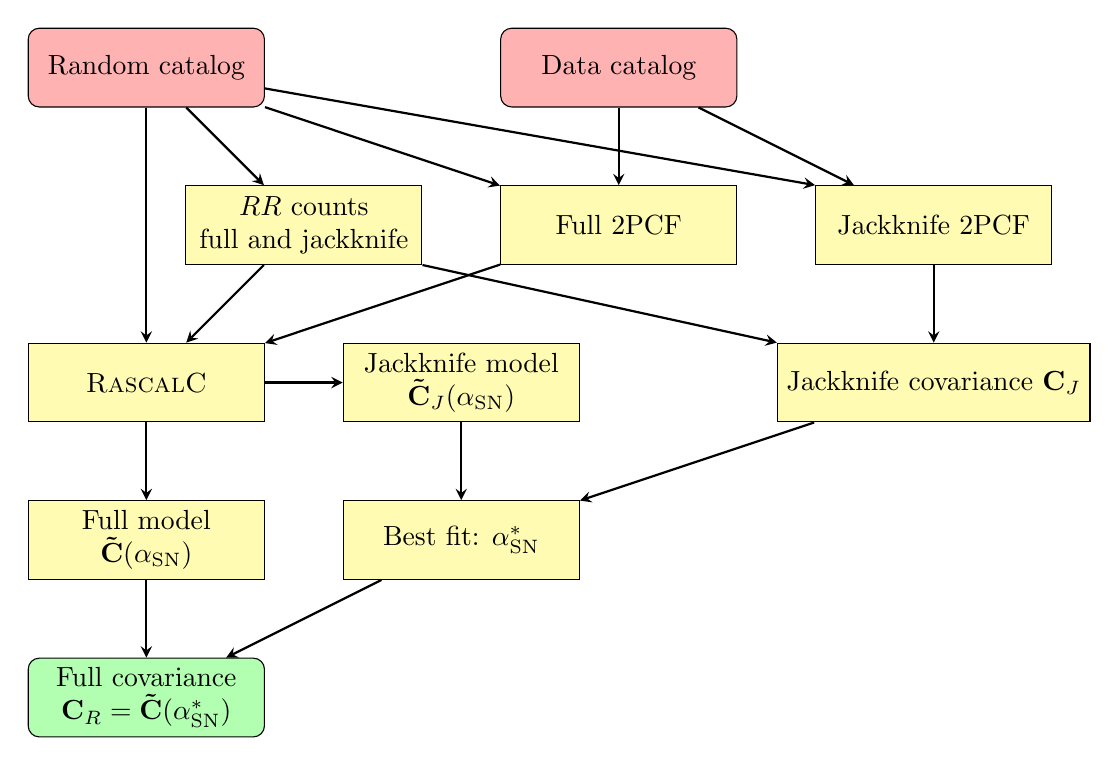
\begin{tikzpicture}[node distance=2cm]
    \node (data) [start] {Data catalog};
    \node (randoms) [start, left of=data, xshift=-4 cm] {Random catalog};
    \node (full_xi) [process, below of=data] {Full 2PCF};
    \node (jack_xi) [process, right of=full_xi, xshift=2 cm] {Jackknife 2PCF};
    \node (RR) [process, left of=full_xi, xshift=-2 cm, align=center] {$RR$ counts\\full and jackknife};
    \node (jack_cov) [process, below of=jack_xi] {Jackknife covariance ${\bf C}_J$};
    \node (RascalC) [process, below of=randoms, yshift=-2 cm] {\rascalc{}};
    \node (jack_model) [process, right of=RascalC, xshift=2 cm, align=center] {Jackknife model\\ ${\bf \tilde C}_J(\snrescaling)$};
    \node (full_model) [process, below of=RascalC, align=center] {Full model\\ ${\bf \tilde C}(\snrescaling)$};
    \node (fit_alpha) [process, below of=jack_model] {Best fit: $\snrescaling^*$};
    \node (full_cov) [stop, below of=full_model, align=center] {Full covariance\\ ${\bf C}_R = {\bf \tilde C}(\snrescaling^*)$};
    \draw [arrow] (data) -- (jack_xi);
    \draw [arrow] (randoms) -- (jack_xi.north west);
    \draw [arrow] (data) -- (full_xi);
    \draw [arrow] (randoms) -- (full_xi);
    \draw [arrow] (randoms) -- (RR);
    \draw [arrow] (jack_xi) -- (jack_cov);
    \draw [arrow] (RR.south east) -- (jack_cov.north west);
    \draw [arrow] (full_xi) -- (RascalC);
    \draw [arrow] (RR) -- (RascalC);
    \draw [arrow] (randoms) -- (RascalC);
    \draw [arrow] (RascalC) -- (jack_model);
    \draw [arrow] (RascalC) -- (full_model);
    \draw [arrow] (jack_model) -- (fit_alpha);
    \draw [arrow] (jack_cov) -- (fit_alpha);
    \draw [arrow] (full_model) -- (full_cov);
    \draw [arrow] (fit_alpha) -- (full_cov);
\end{tikzpicture}

    \caption[\rascalc{} jackknife (fiducial) pipeline flowchart]{Flowchart of \rascalc{} jackknife pipeline (fiducial; developed in \cite{rascal-jackknife,rascalC}).
    This process is used for DESI data and most of the mock tests in this paper.
    In the latter case, a single mock catalog and its corresponding random catalog(s) are provided as data and randoms.}
    \label{fig:pipeline-jack}
\end{figure}

We start with a summary of the methodology developed in \cite{rascal,rascal-jackknife,rascalC}.
The \rascalc{} code builds single-parameter\footnote{For single tracer; for multiple tracers it is one parameter per tracer.} covariance matrix models\footnote{This step is the most computationally heavy and is implemented in C++.} based on a random catalog and a table of 2-point correlation function values.
Then we fit a model to a reference covariance (defined later) to obtain the optimal parameter value for the final prediction.
In the fiducial data pipeline, shown schematically in \cref{fig:pipeline-jack}, we measure the correlation function directly from the data, the code produces separate models for full and jackknife covariance matrices, we fit the latter to the data jackknife covariance matrix, and plug the resulting optimal parameter into the full model.
\cref{fig:pipeline-mocks} shows an alternative pipeline where we use the best fit of the full covariance model to the mock sample covariance instead.
The jackknife methodology has a significant advantage: it only requires mocks for the initial validation, and then allows to generate covariance matrices for different setups without additional simulations.
We now provide more details on both pipelines, focusing on the single-tracer case; the generalization to multiple tracers can be found in \cref{sec:cov-estimation-extra}.

\begin{figure}[tb!]
    \centering
    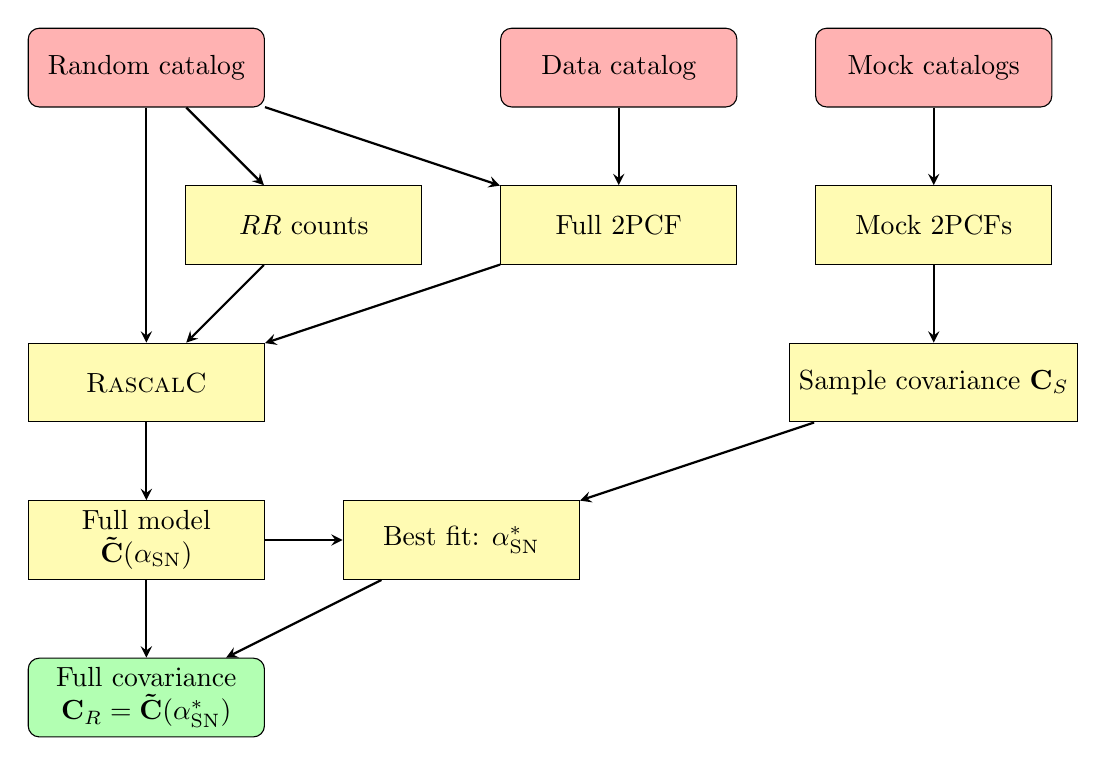
\begin{tikzpicture}[node distance=2cm]
    \node (data) [start] {Data catalog};
    \node (randoms) [start, left of=data, xshift=-4 cm] {Random catalog};
    \node (mocks) [start, right of=data, xshift=2 cm] {Mock catalogs};
    \node (mock_xis) [process, below of=mocks] {Mock 2PCFs};
    \node (full_xi) [process, left of=mock_xis, xshift=-2 cm] {Full 2PCF};
    \node (RR) [process, left of=full_xi, xshift=-2 cm, align=center] {$RR$ counts};
    \node (mock_cov) [process, below of=mock_xis, align=center] {Sample covariance ${\bf C}_S$};
    \node (RascalC) [process, below of=randoms, yshift=-2 cm] {\rascalc{}};
    \node (full_model) [process, below of=RascalC, align=center] {Full model\\ ${\bf \tilde C}(\snrescaling)$};
    \node (fit_alpha) [process, right of=full_model, xshift=2 cm] {Best fit: $\snrescaling^*$};
    \node (full_cov) [stop, below of=full_model, align=center] {Full covariance\\ ${\bf C}_R = {\bf \tilde C}(\snrescaling^*)$};
    \draw [arrow] (mocks) -- (mock_xis);
    \draw [arrow] (data) -- (full_xi);
    \draw [arrow] (randoms) -- (full_xi);
    \draw [arrow] (randoms) -- (RR);
    \draw [arrow] (mock_xis) -- (mock_cov);
    \draw [arrow] (full_xi) -- (RascalC);
    \draw [arrow] (RR) -- (RascalC);
    \draw [arrow] (randoms) -- (RascalC);
    \draw [arrow] (RascalC) -- (full_model);
    \draw [arrow] (full_model) -- (fit_alpha);
    \draw [arrow] (mock_cov) -- (fit_alpha);
    \draw [arrow] (full_model) -- (full_cov);
    \draw [arrow] (fit_alpha) -- (full_cov);
\end{tikzpicture}

    \caption[\rascalc{} mocks (alternative) pipeline flowchart]{Flowchart of \rascalc{} mocks pipeline (alternative; principal idea from \cite{rascal}).
    % Here, it is only used for additional tests on mocks (in \cref{sec:shot-noise-rescaling-values}).
    % In this case, a single mock catalog and its corresponding random catalog(s) are provided as data and randoms.
    The full covariance model can be reused from a jackknife computation (\cref{fig:pipeline-jack}), provided that the randoms and full 2PCF were the same.}
    \label{fig:pipeline-mocks}
\end{figure}

To explain the covariance matrix model, we need to start with the definition of the 2-point correlation function (2PCF).
The standard Landy-Szalay estimator \citep{Landy-Szalay} in radial bin $a$ and angular bin $c$\footnote{\rascalc{} assumes uniform binning in $\abs{\mu}$, $\mu$ being the cosine of the angle between the line of sight and the pair separation (assuming symmetry with respect to $\mu \rightarrow -\mu$). The line of sight is the direction to the midpoint of the galaxy pair in an aperiodic survey, and a fixed coordinate direction ($\hat z$) in periodic boxes.} is
\begin{equation} \label{eq:Landy-Szalay-binned}
\hat\xi_a^c = \frac{\qty(NN)_a^c}{\qty(RR)_a^c}
\end{equation}
where $N=D-R$, $R$ are random points and $D$ are data points (galaxies).

The random counts $RR$ are determined by the survey geometry.
We assume that the survey design choices are independent of the random realization of the Universe.
Consequently, we treat the random counts as fixed.

The numerator, however, is determined by structure formation processes, which are considered stochastic in the cosmological paradigm.
Therefore, it is crucial for scatter in the correlation function measurements.

The $NN$ counts can be expanded as
\begin{equation} \label{eq:NN-RR-discrete}
\qty(NN)_a^c = \sum_{i\neq j}n_i n_j w_i w_j \Theta^a(r_{ij}) \Theta^c(\mu_{ij}) \delta_i \delta_j.
\end{equation}
The survey has been divided into cells indexed by $i$ and $j$.
$n_i$ is the ensemble average number of galaxies in the cell $i$, $w_i$ is the weight for the random point in the cell, $\delta_i$ is the fractional galaxy overdensity in the cell, $\mu_{ij}$ is the absolute value of the cosine of the angle between the line of sight and the separation vector $\vec r_{ij} = \vec r_i - \vec r_j$, $r_{ij}$ is the length of that vector, and $\Theta$ are binning functions (unity if the argument fits into the bin and zero otherwise).

Hereafter, we use the following shorthand notation for the covariance matrix:
\begin{equation} \label{eq:cov2x2_def}
C_{ab}^{cd} \equiv \cov \qty[\hat\xi_a^c, \hat\xi_b^d] \equiv \ev{\hat\xi_a^c \hat\xi_b^d} - \ev{\hat\xi_a^c} \ev{\hat\xi_b^d}.
\end{equation}

This covariance matrix involves an ensemble average of 4 overdensities at up to 4 different positions.
The reason is that each correlation function estimator (\cref{eq:Landy-Szalay-binned,eq:NN-RR-discrete}) contains 2 overdensities at 2 different positions, and they are substituted into \cref{eq:cov2x2_def}.
Some of the 4 positions can be the same, resulting in only 3 or 2 distinct positions\footnote{However, all 4 cannot be the same, because the correlation at zero separation is excluded ($i\ne j$ in \cref{eq:NN-RR-discrete}).} \citep{rascal}.

We then use the following shot-noise approximation to eliminate repeated overdensities at the same position and arrive at the $N$-point correlation functions \cite{rascal}:
\begin{equation} \label{eq:shot-noise-approximation}
\qty(\delta_i)^2 \approx \frac{\snrescaling}{n_i} \qty(1+\delta_i).
\end{equation}
The original motivation \citep{rascal} refers to the Poisson sampling.
We repeat it with slight modifications because the approximation is crucial to the method.
Assuming similar weights for galaxies and randoms, the overdensity in cell $i$ is
\begin{equation} \label{eq:cell-overdensity}
    \delta_i = \frac{b_i}{n_i} - 1,
\end{equation}
where $b_i$ is the actual number of galaxies in the cell and $n_i=\ev{b_i}$ is the expectation value (ensemble average) of that number\footnote{$n_i$ can vary from cell to cell.}.
We can choose a sufficiently small cell size so that $n_i\ll 1$.
Assuming that the galaxies appear in the cell independently, $b_i$ follows the Poisson distribution, and then $\ev{b_i^2}=n_i$.
Substituting \cref{eq:cell-overdensity} into \cref{eq:shot-noise-approximation} and taking the ensemble average of both sides gives $1/n_i - 1 \approx \snrescaling/n_i$.
This sets the baseline expectation for $\snrescaling=1$.

We further explain the overdensity $\delta_i$ in the right-hand side of \cref{eq:shot-noise-approximation}, because it cancels in the previous argument.
With $n_i\ll 1$, the average of $\qty(\delta_i)^2$ is dominated by cells with $b_i=1$.
Whereas almost all the cells have $b_i=0$, the corresponding $\qty(\delta_i)^2=1$ (\cref{eq:cell-overdensity}).
The fraction of cells with $b_i=1$ is only $\approx n_i$, but they have a large $\qty(\delta_i)^2 \approx 1/n_i^2$.
For $b_i=2$, the fraction drops significantly to $\approx n_i^2$, whereas the $\qty(\delta_i)^2 \approx 4/n_i^2$ does not increase as much.
The contributions to the average of $\qty(\delta_i)^2$ (fraction of cells times the $\qty(\delta_i)^2$ value) decrease further for higher values of $b_i$.
Thus substituting the most significant case, $b_i=1$, into \cref{eq:cell-overdensity,eq:shot-noise-approximation} gives $1/n_i^2 - 2/n_i + 1 \approx \snrescaling/n_i^2$.
This is again true for $\snrescaling=1$ because $n_i\ll 1$.
The right-hand side of \cref{eq:shot-noise-approximation} is dominated by $\delta_i\gg 1$ for $b_i=1$, therefore, this overdensity is necessary.

Several factors can cause the shot-noise rescaling, i.e., effectively shift $\snrescaling$ from 1.
First, the observations of galaxies in the same small volume of a real survey are not independent.
There are fundamental limitations to their number due to resolution, number of observations, and number and size of optical fibers in a fiber spectroscopic instrument.
Furthermore, in DESI, each fiber is attached to a robotic positioner confined to a specific area of the focal plane \citep{FocalPlane.Silber.2023}.
Therefore, the selection of a target for the fiber (fiber assignment) must depend on other objects present within this patrol area.
As a result, the number of observed galaxies $b_i$ is not guaranteed to follow the Poisson distribution, and $\ev{b_i^2}=n_i$ may not hold.
Second, different weights on galaxies and random points can alter the cell overdensity estimate $\delta_i = b_i/n_i - 1$.
Such weighting is introduced, in particular, for the mitigation of fiber assignment effects on DESI clustering measurements \citep{KP3s6-Bianchi,KP3s15-Ross}.
The combination of these effects can decrease or increase the shot-noise rescaling.

To recapitulate, the shot-noise approximation (\cref{eq:shot-noise-approximation}) allows us to remove the repeated same-cell overdensities from the covariance matrix estimator.
The ensemble averages of a product of overdensities at $N$ different positions are the $N$-point correlation function by definition.
Therefore, the resulting expression for the covariance matrix involves certain sums with the 4-, 3- and 2-point correlation functions.
We separate the model covariance matrix into three parts:
\begin{equation} \label{eq:Cov2x2estimator}
\tilde C_{ab}^{cd} \qty(\snrescaling) = {^4C}_{ab}^{cd} + \snrescaling {^3C}_{ab}^{cd} + \snrescaling^2 {^2C}_{ab}^{cd}.
\end{equation}
These parts, or the $d$-point terms $^d {\bf C}$ have the following theoretical expressions\footnote{In the \rascalc{} code $^d {\bf C}$ are estimated using Monte Carlo importance sampling of points from random catalogs \citep{rascalC}.}:
\begin{align} \label{eq:Cov2x2_234_Point_Defs}
{^4C}_{ab}^{cd} &= \frac{1}{\qty(RR)_a^c \qty(RR)_b^d} \sum_{i\neq j\neq k\neq l} n_i n_j n_k n_l w_i w_j w_k w_l \Theta^a(r_{ij}) \Theta^c(\mu_{ij}) \Theta^b(r_{kl}) \Theta^d(\mu_{kl}) \\ \nonumber
& \times \qty[\cancel{\eta^{({\rm c})}_{ijkl}} + 2 \xi_{ik} \xi_{jl}] \\ \nonumber
{^3C}_{ab}^{cd} &= \frac{4}{\qty(RR)_a^c \qty(RR)_b^d} \sum_{i\neq j\neq k} n_i n_j n_k w_i w_j^2 w_k \Theta^a(r_{ij}) \Theta^c(\mu_{ij}) \Theta^b(r_{jk}) \Theta^d(\mu_{jk}) \\ \nonumber
& \times \qty[\cancel{\zeta_{ijk}} + \xi_{ik}] \\ \nonumber
{^2C}_{ab}^{cd} &= \frac{2\delta^{ab}\delta^{cd}}{\qty[\qty(RR)_a^c]^2} \sum_{i\neq j} n_i n_j w_i^2 w_j^2 \Theta^a(r_{ij}) \Theta^c(\mu_{ij}) \qty[1+\xi_{ij}],
\end{align}
where $\delta^{ab}$ and $\delta^{cd}$ are Kronecker deltas; $\xi_{ij} = \xi\qty(r_{ij}, \mu_{ij})$ is the 2PCF evaluated\footnote{To compute $\xi_{ij}$, the \rascalc{} code builds a bicubic interpolator based on an input grid of $\xi\qty(r, \mu)$ values.} at the separation between points number $i$ and $j$.

$\zeta_{ijk}$ and $\eta^{{(\rm c)}}_{ijkl}$ are the 3-point and connected 4-point correlation functions.
They are evaluated at the separations between $i,j,k$ and $i,j,k,l$ points, respectively.
These non-Gaussian higher-point functions are included in the theoretical expression for completeness.
However, evaluating them in practice is challenging.
Theoretical models may not cover the necessary range of scales and might also require additional assumptions.
Direct measurements from data are costly and noisy because the number of bins increases for higher-point correlation functions.
Consequently, the 3- and connected 4-point correlation functions are not used in the practical implementation.

Instead of evaluating them, the covariance matrix has been adjusted with the shot-noise rescaling parameter according to \cref{eq:Cov2x2estimator}.
The $d$-point terms have been computed solely with the 2-point function (as designated by crossing out $\zeta$ and $\eta$ in \cref{eq:Cov2x2_234_Point_Defs}).
This 2PCF may, however, include non-linear effects, e.g., due to being estimated from the data or a realistic simulation.

The resulting expressions are theoretically analogous to the Gaussian covariances, neglecting the trispectrum contribution and super-sample covariance \citep[e.g.,][]{gaussian-covariances-galaxy-clustering}.
With them, one can also rescale the shot noise as a free parameter.
The constant shot-noise term in the power spectrum corresponds (via the Fourier transform) to a delta-function addition to the correlation function (which is not commonly considered because we do not measure the correlation function at zero separation).
One can then eliminate the delta functions by integrating their contributions to the full 4-point covariance matrix integral over 1 or 2 of the positions and obtain the 3- and 2-point integrals analogous to sums in \cref{eq:Cov2x2_234_Point_Defs}.
The only difference we found is that the $1+\xi_{ij}$ factor does not appear in the 2-point term ${^2C}_{ab}^{cd}$.
But working in configuration space is advantageous because it allows to naturally account for survey geometry and selection, including the variation of the expected density $\bar n$ across the survey volume, by sampling points from the random catalog.

%\subsection{Mocks}

The key shot-noise rescaling parameter value can be chosen to optimally match a reference covariance obtained from a set of mocks.
The best match is quantified by minimal Kullback-Leibler divergence\footnote{Which is determined by the covariance matrices for two multivariate normal distributions with the same mean.}:
\begin{equation} \label{eq:D_KL-fit-mocks}
    D_{\rm KL} \qty[{\bf \tilde C}^{-1}\qty(\snrescaling), {\bf C}_S] = \frac12 \qty[\tr({\bf \tilde C}^{-1}\qty(\snrescaling) {\bf C}_S) - N_{\rm bins} - \ln \det({\bf \tilde C}^{-1}\qty(\snrescaling) {\bf C}_S)].
\end{equation}
In its computation, the model covariance ${\bf \tilde C}\qty(\snrescaling)$ (with elements given by \cref{eq:Cov2x2estimator}) is inverted because the sample covariance of the simulations ${\bf C}_S$ is more noisy.
With a smooth theoretical model and only one parameter ($\snrescaling$) to adjust, fewer mocks are required than for direct use of their sample covariance matrix \citep{rascal}.
The process is illustrated in \cref{fig:pipeline-mocks}.
In other words, fitting the \rascalc{} covariance model to mocks is akin to template-based smoothing of the simulation-based sample covariance matrix.

Theoretically, the inversion of the \rascalc{} covariance gives a slightly biased estimate of the precision matrix.
However, the Hartlap factor \citep{hartlap-factor} is not applicable since it is not a sample covariance.
The relevant second-order bias correction matrix accounting for importance sampling noise has been worked out \citep{rascal-jackknife}:
\begin{align} \label{eq:bias-correction}
{\bf \tilde \Psi} =& ({\bf \mathbb I} - {\bf \tilde D}) {\bf \tilde C}^{-1} \\ \nonumber
{\bf \tilde D} =& \frac{N_\mathrm{subsamples}-1}{N_\mathrm{subsamples}} \Args{-{\bf \mathbb{I}}+\frac{1}{N_\mathrm{subsamples}}\sum_{i=1}^{N_\mathrm{subsamples}} {\bf \tilde C}_{[i]}^{-1} {\bf \tilde C}_i},
\end{align}
which uses the partial covariance estimates ${\bf \tilde C}_i$ from $N_\mathrm{subsamples}$ distinct sets of configurations resulting from importance sampling in the estimation of sums (Eq.~\eqref{eq:Cov2x2_234_Point_Defs} or \eqref{eq:Cov2x2_234_Point_Defs-jack}) and mean of all the partial estimates but the $i$'th ${\bf \tilde C}_{[i]}$.
However, we find it practically insignificant: the eigenvalues of ${\bf \tilde D}$ are $\lesssim 10^{-3}$.

Unfortunately, the mock-fitting approach does not solve all issues with the mocks.
The simulations still take extra time to produce and impose further assumptions and approximations.
Therefore, a different method is desirable to reduce the dependence on simulations.

%\subsection{Jackknife}

An alternative reference covariance can be obtained from the data with jackknife resampling.
However, the jackknife covariance matrix is not perfectly representative of the true, full-survey covariance for several reasons.
First, the resampled pieces of realistic data have different geometry from the full dataset and each other, which affects the covariance in a complicated way.
Second, the pieces of the data are correlated \citep{MP21,fitted-jk}.
Therefore, it is safer to develop a separate theoretical model for jackknife covariance \citep{rascal-jackknife}, which we briefly explain in the following.

The method uses a slightly non-standard formalism, dubbed {\it unrestricted jackknife} \citep{rascalC}.
Ther,e the jackknife correlation function estimate $\xi_A$ is not the auto-correlation of the whole survey excluding the jackknife region $A$ (as in exclude-one, {\it restricted} jackknife), but the cross-correlation function between that region and the whole survey.
Equivalently, this means that the additional jackknife weighting factor for the pair of points $i,j$, $q^A_{ij}$, is 1 if both of them belong to the jackknife region $A$, $1/2$ if only one, and 0 if neither.
The pair counts can be converted from different terms (auto and cross jackknife counts), often saved separately in light of Mohammad-Percival correction \citep{MP21}.

The unrestricted jackknife is convenient since the full pair counts of each type are the sum of all the jackknife pair counts of the same type.
Then if one weights the regions by the $RR$ pair counts,
\begin{equation} \label{eq:jack-weights}
\qty(w_A)_a^c = \frac{\qty(RR_A)_a^c}{\qty(RR)_a^c},
\end{equation}
the weighted mean correlation function is equal to the full-survey one.
This simplifies the theoretical modeling of the jackknife covariance.

The data jackknife covariance estimate is then
\begin{equation} \label{eq:cov-jackknife-def}
\qty(C_J)_{ab}^{cd} = \frac{\sum_A \qty(w_A)_a^c \qty(w_A)_b^d \qty[\qty(\hat\xi_A)_a^c - \hat\xi_a^c] \qty[\qty(\hat\xi_A)_b^d - \hat\xi_b^d]}{1 - \sum_A \qty(w_A)_a^c \qty(w_A)_b^d},
\end{equation}
the corresponding theoretical estimate, $\qty(\tilde C_J)_{ab}^{cd}$, is constructed analogously to \cref{eq:Cov2x2estimator}:
\begin{equation} \label{eq:Cov2x2estimator-jack}
\qty(\tilde C_J)_{ab}^{cd} \qty(\snrescaling) = \qty(^4C_J)_{ab}^{cd} + \snrescaling \qty(^3C_J)_{ab}^{cd} + \snrescaling^2 \qty(^2C_J)_{ab}^{cd}.
\end{equation}
with terms defined as \citep{rascalC}:
\begin{align} \label{eq:Cov2x2_234_Point_Defs-jack}
\qty(^4C_J)_{ab}^{cd} &= \frac{1}{\qty(RR)_a^c \qty(RR)_b^d \qty[1 - \sum_A \qty(w_A)_a^c \qty(w_A)_b^d]} \sum_{i\neq j\neq k\neq l} n_i n_j n_k n_l w_i w_j w_k w_l \\ \nonumber
& \times \Theta^a(r_{ij}) \Theta^c(\mu_{ij}) \Theta^b(r_{kl}) \Theta^d(\mu_{kl}) \qty[\cancel{\eta^{({\rm c})}_{ijkl}} + \xi_{ij} \xi_{kl} + 2\xi_{ik} \xi_{jl}] \qty(\omega_{ijkl})_{ab}^{cd} \\ \nonumber
\qty(^3C_J)_{ab}^{cd} &= \frac{4}{\qty(RR)_a^c \qty(RR)_b^d \qty[1 - \sum_A \qty(w_A)_a^c \qty(w_A)_b^d]} \sum_{i\neq j\neq k} n_i n_j n_k w_i w_j^2 w_k \\ \nonumber
& \times \Theta^a(r_{ij}) \Theta^c(\mu_{ij}) \Theta^b(r_{jk}) \Theta^d(\mu_{jk}) \qty[\cancel{\zeta_{ijk}} + \xi_{ik}] \qty(\omega_{ijjk})_{ab}^{cd} \\ \nonumber
\qty(^2C_J)_{ab}^{cd} &= \frac{2\delta^{ab}\delta^{cd}}{\qty[\qty(RR)_a^c]^2 \qty{1 - \sum_A \qty[\qty(w_A)_a^c]^2}} \sum_{i\neq j} n_i n_j w_i^2 w_j^2 \Theta^a(r_{ij}) \Theta^c(\mu_{ij}) \qty[1+\xi_{ij}] \qty(\omega_{ijij})_{ab}^{cd},
\end{align}
where $\qty(\omega_{ijkl})_{ab}^{cd}$ is an additional jackknife weight tensor:
\begin{equation}
\qty(\omega_{ijkl})_{ab}^{cd} = \sum_A \qty[q^A_{ij} - \qty(w_A)_a^c] \qty[q^A_{kl} - \qty(w_A)_b^d].
\end{equation}

To sum up, in the fiducial (jackknife) pipeline (\cref{fig:pipeline-jack}), we obtain the shot-noise rescaling by fitting the model for its jackknife covariance (\cref{eq:Cov2x2estimator-jack,eq:Cov2x2_234_Point_Defs-jack}) to the data (\cref{eq:cov-jackknife-def}).
As in the mock approach, this specifically means minimizing the Kullback-Leibler (KL) divergence between the covariance matrices:
\begin{equation} \label{D_KL-fit-jack}
    D_{\rm KL} \qty[{\bf \tilde C}_J^{-1}\qty(\snrescaling), {\bf C}_J] = \frac12 \qty[\tr({\bf \tilde C}_J^{-1}\qty(\snrescaling) {\bf C}_J) - N_{\rm bins} - \ln \det({\bf \tilde C}_J^{-1}\qty(\snrescaling) {\bf C}_J)].
\end{equation}
where the model jackknife covariance ${\bf \tilde C}_J\qty(\snrescaling)$ (\cref{eq:Cov2x2estimator-jack}) is inverted \citep{rascalC}, because the data jackknife covariance matrix ${\bf C}_J$ (\cref{eq:cov-jackknife-def}) is often not invertible.
The final covariance is obtained by plugging the resulting shot-noise rescaling values into the full covariance model (\cref{eq:Cov2x2estimator}).

To summarise, the key assumption is that shot-noise rescaling of purely Gaussian contributions (i.e., ignoring 3-point and connected 4-point functions) can produce a realistic covariance matrix in configuration space.
A theoretical motivation is that non-Gaussian contributions primarily affect the squeezed configurations involving small-scale correlations, below the bin width for the 2-point function, therefore not distinguishable from shot noise operating on infinitesimally small scales.
The method has been empirically shown to agree well with mock-based covariances \citep{rascal,SDSS-rascal,KP4s7-Rashkovetskyi}.

\subsection{Split random-random computation}
\label{sec:split-RR}

\citet{split-randoms} showed that splitting the random catalog into a number of sub-catalogs of the same size as the data catalog when calculating random–random pairs and excluding pairs across different sub-catalogs provides the optimal error at a fixed computational cost.
The splitting can be used in \rascalc{}.
It gives little to no speed-up and impact on results because the importance sampling is too far from complete.
However, it can be useful for multi-node parallelization.
This approach has been used for the data-based \rascalc{} computation in \cite{BAO.EDR.Moon.2023}.

A robust implementation of split random-random pair calculations in \rascalc{} would require considering only quadruples of random points where members of each pair are from the same sub-catalog, but the pairs can be from different catalogs.
However, this has been found to have little to no impact on the results, probably due to the fact that importance sampling covers only a small fraction of all possible configurations.
At the same time, such implementation makes the code less efficient and makes it impossible to split the computation of different catalogs between nodes.

\subsection{Reconstructed two-point function covariance}
\label{subsec:post-recon}

Standard BAO reconstruction modifies the correlation function estimator and thus requires adjustments in the covariance.
Standard BAO reconstruction procedures shift the positions of both the data and random points.
Only shifted data ($D$) is used, whereas the randoms are kept in two variants: original ($R$) and shifted ($S$).
The correlation function is estimated via the Landy-Szalay estimator (\cref{eq:Landy-Szalay-binned}) with $N=D-S$ instead of $D-R$, but still $RR$ in the denominator.
This means shifted randoms are to be used in sums representing $NN$ (starting from \cref{eq:NN-RR-discrete}).
Through the expansion of \cref{eq:cov2x2_def} these propagate into the sums for the covariance matrix terms (\cref{eq:Cov2x2_234_Point_Defs,eq:Cov2x2_234_Point_Defs-jack}).

Thus in the computations of the covariance matrix terms (\cref{eq:Cov2x2_234_Point_Defs,eq:Cov2x2_234_Point_Defs-jack}) for reconstructed catalogs we use
\begin{itemize}
    \item the shifted randoms $S$ in the sums (i.e. $\bm r_i, \bm r_j, \bm r_k, \bm r_l$ used for binning functions and correlation function interpolation are the shifted random positions) because they come from expanding $NN$, which now involves $S$ and not $R$;
    \item non-shifted random counts (i.e., still $RR$) for normalization\footnote{Or correction function(s) in the original implementation of Legendre moments.};
    \item two-point correlation functions $\xi_{ij}$ etc. with a different normalization\footnote{In the code, this is implemented by renormalizing the input grid of correlation values $\xi\qty(r, \mu)$.}: having $SS$ instead of $RR$ in the denominator, i.e.
    \begin{equation} \label{eq:Landy-Szalay-binned-post-input}
    \qty(\hat\xi_{\rm in})_a^c = \frac{\qty(NN)_a^c}{\qty(SS)_a^c}.
    \end{equation}
\end{itemize}
For data jackknife covariance (\cref{eq:cov-jackknife-def}), we still use the ordinary normalization of 2PCF (\cref{eq:Landy-Szalay-binned} with $RR$ in the denominator but $N=D-S$ instead of $D-R$).

In this approach, we treat the shifted randoms as fixed independently of the realization of the Universe's density field.
This is not precisely true because the shifts applied to these randoms depend on the data (observed galaxies).
However, this should be a small effect, because we find the resulting covariances match the mock-based ones well.

% \misha{How this changed with DESI Y1? Although it is not relevant for the \rascalc{}-specific paper}
Shifted randoms are individual for each mock catalog.
Therefore, they can not be defined clearly for mock-averaged computations.
In those cases, we continue to use the non-shifted randoms everywhere for consistency.

\subsection{Revisited covariance for projected Legendre moments of 2PCF}
\label{sec:cov-estimation-new}

Theoretical models of large-scale structure often use multipole (Legendre) moments of the 2-point correlation function instead of its angularly ($\mu$) binned estimates (e.g. \cite{using-CF-multipoles-SDSS-LRG,KP4s2-Chen}).
Moreover, the number of multipoles of interest is typically low --- monopole, quadrupole, and sometimes hexadecapole \citep{KP5s1-Maus,KP5s2-Maus,KP5s3-Noriega,KP5s4-Lai,KP5s5-Ramirez}\footnote{These references discuss the power spectrum modeling, but the $\ell$'th Legendre moment of the correlation function $\xi_\ell$ is determined only by the same-order multipole of the power spectrum $P_\ell$ via a spherical Bessel $j_\ell$ transform.}.
It is then convenient to compress the correlation by converting the angularly-binned correlation function (with more than 3 angular bins) to the Legendre moments.
Covariance matrices for Legendre multipoles have a lower dimension, which causes fewer numerical problems and makes them easier to estimate directly.

The covariance matrix model for Legendre moments was developed in \rascalc{} previously \citep{rascalC-legendre-3}, but this implementation has several disadvantages.

First, it is not directly compatible with jackknives.
In practice, producing the Legendre moment covariance with optimal shot-noise rescaling based on data (not relying on a mock sample) requires two separate computations: one for angular ($\mu$) bins with jackknives to tune the shot-noise rescaling, and another to construct the full covariance matrix model for Legendre multipoles.
This is an inconvenience when one does not intend to use the angularly-binned correlation function in cosmological inference.

Second, the 2PCF estimation library used in DESI, \pycorr{}\footnote{\url{https://github.com/cosmodesi/pycorr}} \citep{pycorr}, operates under slightly different assumptions.
\pycorr{} uses the angularly binned 2-point correlation function $\hat\xi_a^c$ (\cref{eq:Landy-Szalay-binned}) estimates with a large but finite number ($\sim 100$) of angular bins to compute the radially binned Legendre moments:
\begin{equation}
    \hat\xi^\ell_a = \qty(2\ell+1) \sum_c \hat\xi_a^c \int_{\Delta\mu_c} d\mu\, L_\ell(\mu) = \sum_c \hat\xi_a^c F^\ell_c; \label{eq:Legendre-from-binned-2PCF}
\end{equation}
where
\begin{equation}
    F^\ell_c \equiv \qty(2\ell+1) \int_{\Delta\mu_c} d\mu\, L_\ell\qty(\mu) \label{eq:Legendre-projection-factors}
\end{equation}
are the projection factors, which do not depend on radial bins or the tracers involved in the correlation function.
The equations above assume even multipole index $\ell$, and binning in $\abs{\mu}\in [0,1]$\footnote{\pycorr{} is capable of binning in $\mu\in [-1,1]$, retaining the sign information. But all auto-correlation functions are necessarily symmetric, and it is easy to ``wrap'' the counts to $\abs{\mu}$ bins in any case as long as the number of $\mu$ bins is even.}.
In contrast, the \rascalc{} estimators developed earlier assume weighting by Legendre polynomials during pair counting \citep{rascalC-legendre-3}.
This is equivalent to using infinitesimally narrow angular bins in \cref{eq:Legendre-from-binned-2PCF}.
The mismatch in assumptions between \pycorr{} and \rascalc{} may not cause significant differences in practice, but it is not desirable.

Third, an additional step was needed to account for realistic survey geometry.
The previous \rascalc{} realization relies on the survey correction function --- the ratio of pair counts in a real survey and a periodic box with the same volume \citep{survey-correction-factor-ref}.
This function needed to be modeled for arbitrary angles ($\abs{\mu}$).
A piecewise-polynomial form has been assumed \citep{rascalC-legendre-3}.
Whereas they explain the need for two different polynomials by the particularly strong redshift-space distortions near the line of sight ($\abs{\mu}=1$), the choice of the partition point\footnote{I.e. the boundary between the two polynomials, where they join continuously and smoothly.} at $\abs{\mu}=0.75$ has not been motivated and may not be the best.
This might be a minor issue as well, but still a source of extra uncertainty.

We have seen an opportunity to address all three issues and streamline the covariance matrix computation procedure for extensive usage with DESI.
Since the projection in \cref{eq:Legendre-from-binned-2PCF} is linear, the covariance matrix for these Legendre moments estimators can be obtained from the $r,\mu$-binned one given by \cref{eq:Cov2x2estimator}:
\begin{equation} \label{eq:full-cov-projection-Legendre}
    \tilde C_{ab}^{\ell\ell'} \equiv \cov \qty[\hat \xi^\ell_a, \hat \xi^{\ell'}_b] = \sum_{c,d} \tilde C_{ab}^{cd} F^\ell_c F^{\ell'}_d.
\end{equation}

A major technical result of this paper is a methodology to compute this covariance matrix of the Legendre multipoles directly at the level of the summation over point configurations, rather than having to compute and then project the much larger covariance matrix of fine angular bins.
For this, several quantities need to be inserted into the sums of \cref{eq:Cov2x2_234_Point_Defs}, and we obtain the following 4, 3, and 2-point terms:
\begin{align} \label{eq:Cov2x2_234_Point_Defs_Legendre_Projected}
{^4C}_{ab}^{\ell\ell'} &= \sum_{i\neq j\neq k\neq l} n_i n_j n_k n_l w_i w_j w_k w_l \Theta^a(r_{ij}) \Theta^b(r_{kl}) \qty[\cancel{\eta^{({\rm c})}_{ijkl}} + 2\xi_{ik} \xi_{jl}] \\ \nonumber
& \times \sum_c \frac{\Theta^c(\mu_{ij}) F^\ell_c}{\qty(RR)_a^c} \sum_d \frac{\Theta^d(\mu_{kl}) F^{\ell'}_d}{\qty(RR)_b^d}, \\ \nonumber
{^3C}_{ab}^{\ell\ell'} &= 4 \sum_{i\neq j\neq k} n_i n_j n_k w_i w_j^2 w_k \Theta^a(r_{ij}) \Theta^b(r_{jk}) \qty[\cancel{\zeta_{ijk}} + \xi_{ik}] \sum_c \frac{\Theta^c(\mu_{ij}) F^\ell_c}{\qty(RR)_a^c} \sum_d \frac{\Theta^d(\mu_{jk}) F^{\ell'}_d}{\qty(RR)_b^d}, \\ \nonumber
{^2C}_{ab}^{\ell\ell'} &= 2\delta^{ab} \sum_{i\neq j} n_i n_j w_i^2 w_j^2 \Theta^a(r_{ij}) \qty[1+\xi^{XY}_{ij}] \sum_c \frac{\Theta^c(\mu_{ij}) F^\ell_c F^{\ell'}_c}{\qty[\qty(RR)_a^c]^2}.
\end{align}
As in \cref{eq:Cov2x2_234_Point_Defs}, we include the non-Gaussian higher-point functions in these theoretical equations.
However, we drop them in the current implementation, which we signify by crossing them out.
Sums like $\sum_c \Theta^c(\mu) \dots$ practically mean finding the angular bin $\tilde c$ to which the $\mu$ value belongs and then evaluating the rest only for that one bin.
Within the code, we sample a quadruplet, triplet, or pair of particles and then accumulate their contribution to all the Legendre multipole moments in their radial bins.

These 4, 3, and 2-point terms can be combined to the full theoretical estimate analogously to \cref{eq:Cov2x2estimator}, i.e.
\begin{equation} \label{eq:cov2x2_Legendre}
\tilde C_{ab}^{\ell\ell'} \qty(\snrescaling) = {^4C}_{ab}^{\ell\ell'} + \snrescaling {^3C}_{ab}^{\ell\ell'} + \snrescaling^2 {^2C}_{ab}^{\ell\ell'}.
\end{equation}
This is the single-tracer expression; the version for multiple tracers is provided in \cref{sec:cov-estimation-multi-legendre-projected}.

For simplicity, we have decided to reuse the $r,\mu$ binned jackknife covariance matrix estimate (\cref{eq:cov-jackknife-def}).
An alternative could be a tedious re-derivation of the theoretical jackknife covariance model with some weights for individual jackknife multipole estimators.
The method only requires this step to calibrate the shot-noise rescaling parameter.
The precise choice of the reference jackknife covariance should not matter as long as the data and model estimators are treated consistently.
Consequently, we project the angularly-binned data jackknife covariance matrix (\cref{eq:cov-jackknife-def}) similarly to the full covariance (\cref{eq:full-cov-projection-Legendre}):
\begin{equation} \label{eq:jack-cov-projection-Legendre}
    \qty(C_J)_{ab}^{\ell\ell'} = \sum_{c,d} \qty(C_J)_{ab}^{cd} F^\ell_c F^{\ell'}_d
\end{equation}
and do the same with the theoretical prediction (\cref{eq:Cov2x2estimator-jack}):
\begin{equation} \label{eq:Cov2x2estimator-jack-legendre}
\qty(\tilde C_J)_{ab}^{\ell\ell'} \qty(\snrescaling) = \qty(^4C_J)_{ab}^{\ell\ell'} + \snrescaling \qty(^3C_J)_{ab}^{\ell\ell'} + \snrescaling^2 \qty(^2C_J)_{ab}^{\ell\ell'}.
\end{equation}
The jackknife $d$-point terms (\cref{eq:Cov2x2_234_Point_Defs-jack}) accordingly are transformed to
\begin{align} \label{eq:Cov2x2_234_Point_Defs-jack-legendre}
\qty(^4C_J)_{ab}^{\ell\ell'} &= \sum_{i\neq j\neq k\neq l} n_i n_j n_k n_l w_i w_j w_k w_l \Theta^a(r_{ij}) \Theta^b(r_{kl}) \qty[\cancel{\eta^{({\rm c})}_{ijkl}} + \xi_{ij} \xi_{kl} + 2\xi_{ik} \xi_{jl}] \\ \nonumber
& \times \sum_{c,d} \frac{\qty(\omega_{ijkl})_{ab}^{cd} \Theta^c(\mu_{ij}) \Theta^d(\mu_{kl}) F^\ell_c F^{\ell'}_d}{\qty(RR)_a^c \qty(RR)_b^d \qty[1 - \sum_A \qty(w_A)_a^c \qty(w_A)_b^d]}, \\ \nonumber
\qty(^3C_J)_{ab}^{\ell\ell'} &= 4 \sum_{i\neq j\neq k} n_i n_j n_k w_i w_j^2 w_k \Theta^a(r_{ij}) \Theta^b(r_{jk}) \qty[\cancel{\zeta_{ijk}} + \xi_{ik}] \\ \nonumber
& \times \sum_{c,d} \frac{\qty(\omega_{ijjk})_{ab}^{cd} \Theta^c(\mu_{ij}) \Theta^d(\mu_{jk}) F^\ell_c F^{\ell'}_d}{\qty(RR)_a^c \qty(RR)_b^d \qty[1 - \sum_A \qty(w_A)_a^c \qty(w_A)_b^d]}, \\ \nonumber
\qty(^2C_J)_{ab}^{\ell\ell'} &= 2\delta^{ab} \sum_{i\neq j} n_i n_j \qty(w_i w_j)^2 \Theta^a(r_{ij}) \qty[1+\xi_{ij}] \sum_c \frac{\qty(\omega_{ijij})_{ab}^{cc} \Theta^c(\mu_{ij}) F^\ell_c F^{\ell'}_c}{\qty[\qty(RR)_a^c]^2 \qty{1 - \sum_A \qty[\qty(w_A)_a^c]^2}}.
\end{align}
Similarly to \cref{eq:Cov2x2_234_Point_Defs_Legendre_Projected}, sums of the form $\sum_{c,d} \Theta^c(\mu_1) \Theta^d(\mu_2) \dots$ practically mean finding the angular bins $\tilde c,\tilde d$ to which the $\mu_{1,2}$ values belong correspondingly and then evaluating the rest ($\dots$) only for that pair of bins.
A given set of cells contributes to the covariance of one pair of angular bins ($c,d$ in \cref{eq:Cov2x2_234_Point_Defs}), but all multipoles ($\ell,\ell'$).

We have also omitted the small disconnected part of the 4-point jackknife term ($\xi_{ij} \xi_{kl}$) in the main code implementation for practical reasons.
This part is estimated in $r,\mu$ bins (\cref{eq:Cov2x2_234_Point_Defs-jack}) by separating it into a product of two sums that need to be computed for each jackknife region \citep{rascalC}.
The evaluation becomes less convenient in Legendre multipoles due to the projection factors inserted into the sum over cells/particles.
We have computed the disconnected term in a couple of realistic setups by using the technique for $r,\mu$ bins\footnote{Storing more data due to keeping many (100) angular ($\mu$) bins for each of 60 jackknife regions. The number of angular bins could be reduced, but at the price of potential loss of precision.} and projecting the resulting covariance matrix part into the multipole moments (analogously to \cref{eq:jack-cov-projection-Legendre}).
We have found that the inclusion of the disconnected term does not change the shot-noise rescaling values up to the 6th digit after the decimal point.
The optimal shot-noise rescaling parameter is the only link between the disconnected jackknife term and the final covariance matrix.
Therefore, we concluded that the impact of the disconnected term is practically negligible.

In addition, we give a theoretical justification for neglecting the disconnected term, although not completely strict.
The disconnected jackknife term vanishes exactly if either the correlation function is constant, the jackknife regions are identical, or the jackknife counts in each region are the same in each fine bin \citep{rascalC}.
An arbitrary survey would not meet any of these conditions exactly, but they likely hold approximately.
Therefore, the disconnected term is expected to be small.

This concludes the description of the new covariance estimators we apply to DESI data and mocks.
To reiterate, the key practical advantage is that a single computation provides the Legendre covariance with shot-noise rescaling tuned on jackknives.
Additionally, the new estimators use the random-random counts directly, instead of relying on a survey correction function fit for realistic survey geometry \citep{rascalC-legendre-3}.
Therefore, we use this method for covariance matrix estimation in the rest of this paper.

\section{Methods of comparison of covariance matrices}
\label{sec:cov-comparison}

Since a covariance matrix is a high-dimensional object, it can be hard to explore and interpret.
Moreover, we run the pipeline multiple times independently and aim to study all the covariance matrix products to assess their stability and fluctuations.
Thus, compact and numerical comparison measures are instructive.

\subsection{Interpretable measures of similarity for covariance matrices (original version, needs to be merged with the other one)}
\label{subsec:comparison-measures}

The first characteristic we consider is the Kullback-Leibler (KL) divergence, a measure of distance between distributions used to fit covariances in \rascalc{} (\cref{sec:cov-estimation-review,eq:D_KL-gaussian}).
It is generally defined as the expectation value of the logarithm of the ratio of the two probability distribution functions according to the first distribution:
\begin{equation} \label{eq:D_KL-definition}
D_{\rm KL} (P_1 || P_2) = \int \ln \Arg{\frac{P_1(x)}{P_2(x)}} P_1(x) dx
\end{equation}
By this expression, KL divergence can be seen as an average difference in log-likelihood.
For two Gaussian distributions with covariance matrices ${\bf C}_i$ and precision matrices ${\bf \Psi}_i={\bf C}_i^{-1}$ describing $N_{\rm bins}$ observables (correlation function bins in our setup), it can be found as
\begin{equation} \label{eq:D_KL-gaussian}
D_{\rm KL} \Arg{{\bf \Psi}_1, {\bf C}_2} = \frac12 \Args{\tr \Arg{{\bf \Psi}_1 {\bf C}_2} - N_{\rm bins} - \ln \det \Arg{{\bf \Psi}_1 {\bf C}_2}}.
\end{equation}
% This is the expression we will use.
The KL divergence computed using the \rascalc{} precision matrix and mock sample covariance is related to the log-likelihood of the sample covariance under the assumption that the \rascalc{} covariance truly describes the distribution of mock clustering measurements\footnote{This log-likelihood relation does not hold if the KL divergence is computed between sample precision (inverse covariance) and theoretical covariance matrices.} \citep{rascal}
This is very appropriate for testing the hypothesis that the \rascalc{} precision matrix is a precise, unbiased estimate.

The next metric assesses how close the first precision matrix is to the inverse of the second covariance matrix, and at the same time, a ``directional'' root-mean-square relative difference in $\chi^2$ given by the two covariance matrices (explained in more detail in \cref{subsec:inv-test}):
\begin{align} \label{eq:R_inv-definition}
R_{\rm inv} \Arg{{\bf \Psi}_1, {\bf C}_2} =& \frac1{\sqrt{N_{\rm bins}}} \Abs{\Abs{{\bf C}_2^{1/2} {\bf \Psi}_1 {\bf C}_2^{1/2} - {\bf \mathbb I}}}_F \nonumber \\
=& \sqrt{\frac{\tr \Args{\Arg{{\bf \Psi}_1 {\bf C}_2 - {\bf \mathbb I}}^2}}{N_{\rm bins}}}.
\end{align}
This measure can also be seen as the average relative difference in the errorbars.
Moreover, if the covariance matrix is estimated from a sample with multivariate normal distribution and the precision matrix is assumed to be true, $R_{\rm inv}^2$ is proportional to the $\chi^2$ computed using the covariance of independent covariance matrix elements (\cref{subsec:inv-test}).
Thus, in this case, it can serve as an approximation of log-likelihood for optimization.

The last metric is akin to the mean reduced $\chi^2$ of samples corresponding to one covariance matrix with respect to the other precision matrix:
\begin{equation} \label{eq:chi2_red-definition}
\chi^2_{\rm red} \Arg{{\bf \Psi}_1, {\bf C}_2} = \frac1{N_{\rm bins}} \tr \Arg{{\bf \Psi}_1 {\bf C}_2}.
\end{equation}
It can be seen as the mean ratio of $\chi^2$ given by the two covariance/precision matrices.

All three metrics are not symmetric, meaning that values for $\Arg{{\bf \Psi}_1, {\bf C}_2}$ and $\Arg{{\bf \Psi}_2, {\bf C}_1}$ may be different, so in principle, it might be informative to consider differences both ways.
On the other hand, the sample covariance is less robust than the \rascalc{} result, and its inversion can be less stable.
Moreover, computing each metric twice makes the results more numerous and less clear.
Finally, some additional properties do not hold with the other one, as noted above.
Therefore, we decided to limit ourselves to \rascalc{} precision matrices and sample covariance matrices.

For a better understanding of the metrics, let us consider the eigenvalues of ${\bf \Psi}_1 {\bf C}_2$ (alternatively, one can use ${\bf \Psi}_1^{1/2} {\bf C}_2 {\bf \Psi}_1^{1/2}$ which is symmetric) and denote them as $\lambda_a$.
We would like ${\bf \Psi}_1 \rightarrow {\bf C}_2^{-1}$ thus all $\lambda_a \rightarrow 1$.
The metrics then can be expressed as
\begin{equation} \label{eq:D_KL-explanation}
D_{\rm KL} \Arg{{\bf \Psi}_1, {\bf C}_2} = \frac12 \sum_{a=1}^{N_{\rm bins}} \left[ \lambda_a - 1 - \ln \lambda_a \right] \approx \frac14 \sum_{a=1}^{N_{\rm bins}} (\lambda_a - 1)^2,
\end{equation}
\begin{equation} \label{eq:R_inv-explanation}
R_{\rm inv} \Arg{{\bf \Psi}_1, {\bf C}_2} = \sqrt{\frac1{N_{\rm bins}} \sum_{a=1}^{N_{\rm bins}} (\lambda_a - 1)^2},
\end{equation}
\begin{equation} \label{eq:chi2_red-explanation}
\chi^2_{\rm red} \Arg{{\bf \Psi}_1, {\bf C}_2} = \frac1{N_{\rm bins}} \sum_{a=1}^{N_{\rm bins}} \lambda_a.
\end{equation}
Thus $D_{\rm KL}$ and $R_{\rm inv}$ accumulate any deviation of $\lambda_a$ from 1, although they cannot indicate the direction of such differences.
Note that the quadratic expression for $D_{\rm KL}$ is approximate, so it is not generally degenerate with $R_{\rm inv}$, although as the covariance matrices approach each other, these two measures become more redundant:
\begin{equation} \label{eq:D_KL-R_inv-redundancy}
D_{\rm KL} \Arg{{\bf \Psi}_1, {\bf C}_2} \approx \frac{N_{\rm bins}}4 R_{\rm inv}^2 \Arg{{\bf \Psi}_1, {\bf C}_2}.
\end{equation}
$\chi^2_{\rm red}$ can show which covariance matrix is ``larger'' on average, while deviations in opposite directions may cancel each other.

Finally, it is important to set expectations for these three comparison measures in the perfect case.
By this, we mean comparing the true precision matrix with the sample covariance estimated from $n_S$ multivariate normal samples following the same covariance.
The distribution of clustering statistics can be assumed normal.
This allows us to test the hypothesis that \rascalc{} can predict the true covariance of the mocks.

In this case, we need to focus on the noise properties of the sample covariance matrix ${\bf C}_S$ obtained via the standard unbiased estimator for the case when the true mean is not known:
\begin{equation} \label{eq:sample-cov}
C_{S,ab} = \frac1{n_S-1} \sum_{i=1}^{n_S} (\xi_{a,i} - \bar \xi_a) (\xi_{b,i} - \bar \xi_b)
\end{equation}
where $a,b$ denote bin numbers, $i,j$ index sample numbers, and $\bar \xi_a$ is the estimate of the mean:
\begin{equation}
\bar \xi_a \equiv \frac1{n_S} \sum_{i=1}^{n_S} \xi_{a,i}.
\end{equation}
Since the clustering measurements are described well by a multivariate normal distribution, their sample covariance matrix follows the Wishart distribution.
This provides a reference of how the metrics behave when the perfect precision matrix is compared to a covariance matrix estimated from $n_S$ samples with $N_{\rm bins}$ bins (or any other Gaussian observables).

Full derivations are presented in \cref{sec:cov-comparison-properties}; here, we will only provide the results for mean/expectation values and standard deviations:
\begin{align} \label{eq:D_KL-stats}
& \Avg{D_{\rm KL} \Arg{{\bf \Psi}_0, {\bf C}_S}} \approx \frac{N_{\rm bins}(N_{\rm bins}+1)}{4(n_S-1)}, \nonumber \\
& \sigma \Args{D_{\rm KL} \Arg{{\bf \Psi}_0, {\bf C}_S}} \approx \frac12 \sqrt{\frac{N_{\rm bins} [(N_{\rm bins} + 1) (n_S + 2 N_{\rm bins} + 2) + 2]}{\Arg{n_S-1}^3}};
\end{align}
\begin{align} \label{eq:R_inv-stats}
& \Avg{R_{\rm inv} \Arg{{\bf \Psi}_0, {\bf C}_S}} \approx \sqrt{\frac{N_{\rm bins}+1}{n_S-1}}, \nonumber \\
& \sigma \Args{R_{\rm inv} \Arg{{\bf \Psi}_0, {\bf C}_S}} \approx \frac1{n_S-1} \sqrt{\frac{(N_{\rm bins} + 1) (n_S + 2 N_{\rm bins} + 2) + 2}{N_{\rm bins} (N_{\rm bins}+1)}}.
\end{align}
Naively, one could expect $D_{\rm KL}$ and $R_{\rm inv}$ to become arbitrarily small as ${\bf \Psi}_1 \rightarrow {\bf \Psi}_0$.
However, in reality, they can have large expectation values, especially as the number of bins increases.

$\chi^2_{\rm red}$, however, would behave like the reduced $\chi^2$ with $N_{\rm bins} \times (n_S-1)$ degrees of freedom in this case (see \cref{subsec:chi2}):
\begin{align} \label{eq:chi2_red-stats}
& \Avg{\chi^2_{\rm red} \Arg{{\bf \Psi}_0, {\bf C}_S}} = 1, \nonumber \\
& \sigma \Args{\chi^2_{\rm red} \Arg{{\bf \Psi}_0, {\bf C}_S}} = \sqrt{\frac2{N_{\rm bins} (n_S-1)}}.
\end{align}
It might seem like $D_{\rm KL}$ and $R_{\rm inv}$ could be unbiased by multiplying one of the matrices by a factor similar to the Hartlap factor \citep{hartlap-factor}, but a lack of bias in $\chi^2_{\rm red}$ expectation value suggests that this is not true.

It is notable that a deviation of $\chi^2_{\rm red}$ from 1 would contribute to $R_{\rm inv}$ -- see \cref{eq:chi2_red-explanation,eq:R_inv-explanation}; their consequence is also that
\begin{equation} \label{eq:chi2_red-R_inv-limit}
\Abs{\chi^2_{\rm red} \Arg{{\bf \Psi}_1, {\bf C}_2} - 1} \le R_{\rm inv} \Arg{{\bf \Psi}_1, {\bf C}_2}.
\end{equation}
However, the direction of such deviation will not be clear in $R_{\rm inv}$, and a nontrivial expectation value can make it harder to interpret.
This keeps $\chi^2_{\rm red}$ useful in many cases.

For additional validation, we also compute the statistical means and standard deviations for our comparison measures empirically (Monte-Carlo method) with a large number of multivariate normal samples.
We generate $N_r=10,000$ chunks of $n_S$ independent samples of $N_{\rm bins}$-dimensional multivariate normal vectors with a (true) unit covariance matrix\footnote{The value of the true covariance matrix does not matter because it cancels out in each comparison measure (ignoring the numerical instabilities).
The dimension, however, is crucially important.
Therefore, we repeat the procedure for each value of $N_{\rm bins}$ relevant for comparisons in this work.}.
In each chunk, we estimate the sample covariance and compute the comparison measures between their true (unit) precision matrix and the sample covariance estimate.
Finally, we estimate the mean and standard deviation for each comparison measure using the obtained $N_r$ random realizations\footnote{These realizations of covariance matrix comparison measures (for $n_S=1000$), as well as all estimates of their means and standard deviations (theoretical, empirical and our fiducial choice between the two for each case), are provided in the supplementary material: \supplementarylink{}.}.
    
We choose a preferred (fiducial) value between the theoretical estimate and the corresponding empirical figure in each case.
We prefer the theoretical value unless the difference is more than $3\sigma$.
Otherwise, we select the empirical estimate.
As suspected, we only find $>3\sigma$ deviations for KL divergence (with larger numbers of bins) and $R_{\rm inv}$ (for smaller numbers of bins).
The fiducial values are used in \cref{tab:cov-comparison-full,tab:cov-comparison-shape-range,tab:cov-comparison-BAO-range,tab:cov-comparison-BAO-parameters,tab:cov-comparison-ShapeFit-parameters,tab:cov-comparison-direct-fit-parameters} as reference for comparison measures between \rascalc{} precision matrices and sample covariances.

\subsection{Internal convergence assessment}
\label{subsec:internal-convergence-metrics}

Internal consistency of \rascalc{} covariance matrices in one run and the convergence of the Monte-Carlo integration procedure are also important to assess quantitatively.
We propose to employ the above-mentioned methods to accomplish this and provide valuable diagnostics that do not rely on a reference (e.g., sample) covariance and thus can be used in any run, including the pure data-based one.
However, we need to note that such a test can only quantify limited sources of uncertainty or error, leaving aside the factors like adequacy of the approximations in the formalism, the precision of the input clustering, and noise in the jackknife covariance estimated from the data.

The \rascalc{} code provides multiple partial intermediate results corresponding to practically non-overlapping sets of quadruples, triples, and pairs of points.
These resulting covariance matrices can be split into two distinct sets of similar size, averaged within them, and compared using the three metrics.
In this case, however, the arguments for the $\chi^2_{\rm red}$ weaken -- we can expect $R_{\rm inv}$ to become arbitrarily low as the number of Monte-Carlo samples increases, which would limit the reduced chi-squared via \cref{eq:chi2_red-R_inv-limit}, and it is not as interesting to understand which of the halves gives a ``smaller'' matrix.
Then $D_{\rm KL}$ also becomes more redundant with $R_{\rm inv}$ via \cref{eq:D_KL-R_inv-redundancy}.
Therefore, it is reasonable to only show $R_{\rm inv}$, which can be seen as an estimate of root-mean-square relative precision (considered over all directions in measurement space).

\subsection{Fisher projection to the space of model parameters}
\label{sec:param-space-fisher}

Comparing the full covariance matrices for observables (e.g., binned 2PCF or 2PCF multipoles) may be overly generic.
In such a case, we consider every arbitrary ``direction'' in the high-dimensional linear space of these observables.
Some of these directions may be unphysical, whereas others can have little or no connection to the data analysis.
To highlight a smaller number of meaningful, impactful directions, \cite{subspace-projection,cov-comparison-projection} suggested projecting the covariance matrices into a model-dependent subspace.

We project the covariance matrices to the model parameters through the inverse of the Fisher matrix for simplicity.
For \rascalc{} results, one can use a simple expression neglecting the inversion bias (Hartlap-like) corrections\footnote{As we mentioned in \cref{sec:cov-estimation-review}, such corrections are small for \rascalc{}.}:
\begin{equation}
{\bf C}_R^{\rm par} = \qty[{\bf M} \qty({\bf C^\prime}^{\rm obs}_R)^{-1} {\bf M}^T]^{-1}. \label{eq:parameter-covariance-rascalc}
\end{equation}
${\bf C^\prime}^{\rm obs}_R$ is the \rascalc{} covariance matrix restricted to the separation and multipole range of the respective model.
This range consitutes $N^\prime_{\rm bins}$ observables.
${\bf M}$ is the Jacobian of the model, i.e., the matrix of derivatives of radially-binned 2PCF multipoles $\bm \xi$ with respect to the parameter vector $\bm \theta$:
\begin{equation}
M_{pa} \equiv \frac{\partial \xi_a}{\partial \theta_p}. \label{eq:model-jacobian}
\end{equation}

For the mock sample covariance, we use a similar expression:
\begin{equation}
{\bf C}_S^{\rm par} = \frac{n_S-1}{n_S-N^\prime_{\rm bins}+N_{\rm pars}-1} \qty[{\bf M} \qty({\bf C^\prime}^{\rm obs}_S)^{-1} {\bf M}^T]^{-1}.  \label{eq:parameter-covariance-sample}
\end{equation}
$n_S$ is the number of mock samples used to estimate the sample covariance, and $N_{\rm pars}$ is the number of model parameters.

The important difference from \cref{eq:parameter-covariance-rascalc} is that the sample covariance estimate is more noisy than the semi-analytical model result.
Therefore, non-linear matrix inversion operations cause significant biases.
\cite{density-split-clustering-constrain-nuLCDM} considered this problem and gave a single (Hartlap-like) correction factor in their Eq.~(B6), which we use here.
The additional multiplier removes the inversion biases to leading order.

In \cref{sec:cov-comparison-param} we additionally exclude the nuisance parameters.
We leave out the corresponding rows and columns from the covariance matrices given by \cref{eq:parameter-covariance-sample,eq:parameter-covariance-rascalc}.
The remaining sub-matrix represents the covariance of the parameters of interest marginalized over the nuisance parameters.

\section{Application to \desimtwo{} LRG mocks}
\label{sec:validation-DESI-M2}

In this section, we use the described methods on \desimtwo{} mocks to assess the performance and stability of the approach on the actual dataset.
We describe the setup first, then perform intrinsic validation described in \cref{subsec:internal-convergence-metrics}, look at the shot-noise rescaling values resulting from jackknife calibration used for the final covariance estimates, validate the \rascalc{} results by comparison with the mock sample covariance in measurement/observable and parameter space and finally focus specifically on errorbars on BAO scale.

\subsection{Mock catalogs and reconstruction method}
\label{subsec:mocks}

We use the 999 effective Zel'dovich (EZ) mocks \citep{EZmocks,EZmocks2021} with cuts corresponding to the DESI LRG sample \citep{LRG.TS.Zhou.2023} (described in more detail in \cite{BAO.EDR.Moon.2023}), which will be referred to as \themocks{}.
Sample covariance based on these does not provide a perfect reference because both the number of mock catalogs and the level of details in each simulation are limited, but the best one can have realistically, because increasing one without making the other worse would require even more significant computational resources.
Comparing these is also robust to the mismatch between the data and mock clustering.

The reconstruction method is also the same as in \cite{BAO.EDR.Moon.2023}: the iterative procedure \citep{recon-fourier-space} implemented in the {\tt IterativeFFTReconstruction} 
algorithm of the {\sc pyrecon} package\footnote{\url{https://github.com/cosmodesi/pyrecon}} with the {\tt RecIso} convention.
%\footnote{\texttt{RecIso} is a choice to remove the large-scale anisotropy due to redshift-space distortions in the process of reconstruction \citep{PadRecIso,SeoBAOmodel2016}.}
Three iterations are used with a Gaussian smoothing kernel of width $15 \ihMpc$. 
An approximate growth rate and the expected bias are assumed.

\subsection{Setup}
\label{subsec:validation-setup}

For this study, we have performed separate runs using 2PCF measured from single LRG \themocks{} catalogs.
%Each represents a fair proxy for the \desimtwo{} data.
This has been repeated 10 times for pre- and post-recon.
In the latter case, individual shifted random catalogs have been used for each mock following the procedure we described in \cref{subsec:post-recon}.
%We have applied the covariance matrix comparison metrics from \cref{sec:cov-comparison}, which consider the full space of possibilities and are more compact at the same time, being just a number between two covariances.

Pre-reconstruction galaxies and randoms were assigned unity weights.
Post-reconstruction, FKP weights \citep{FKP} were used, given by
\begin{equation}
    w_{\rm FKP} = \frac{1}{1+n(z) C P_0}
\end{equation}
where $n(z)$ is the weighted number density (per volume),
$C$ is the mean completeness for the sample,
and $P_0$ is a fiducial power-spectrum amplitude.
For LRG, $C=0.579$ and $P_0=10^4 (\ihMpc)^3$ \citep{BAO.EDR.Moon.2023}.
We note that the weighting schemes are not exactly the same as for real data, but since weights are included explicitly in the covariance estimators, we expect \rascalc{} to work with any fixed choice applied consistently for 2PCF measurements and Monte-Carlo integration.

For the importance sampling input, 10 random catalogs were used in pre-recon computations and 20 in post-recon, like for the $RR$ ($SS$) pair counts computation for the 2PCF estimates.
These randoms have been concatenated before being provided to \rascalc{} executable.
%They have been used disjointly as described in \cref{sec:disjoint-RR}.
We assign 60 jackknife regions assigned by a $K$-means subsampler based on data positions (but not weights) as in \desimtwo{} data, compute the jackknife covariance matrix and use it to calibrate the shot-noise rescaling.

We note that some validation has been performed in \cite{BAO.EDR.Moon.2023}: \rascalc{} covariance matrix based on 2PCF averaged over all LRG \themocks{} with no shot-noise rescaling applied (and using unshifted randoms in the post-reconstruction case) has been compared to the sample covariance matrix in terms of $\chi^2$ of BAO fits, best-fit values and standard deviations of BAO isotropic scale parameter $\alpha$, yielding a good agreement.
However, there are significant limitations to this approach:
\begin{itemize}
\item effect of noise in the input clustering is significantly smaller in 2PCF averaged over $\approx 1000$ mocks than in the real data, which is close to a single mock catalog;
\item possible differences in other parameters of the BAO model or more generic aspects of the correlation function have not been assessed.
\end{itemize}
Single-mock runs address the first issue since each of them is a fair proxy of the data.
The use of covariance matrix comparison metrics from \cref{subsec:comparison-measures} expands on the second one.
We keep the result with mock-average 2PCF, labeled ``Average G'' (Gaussian), to assess the importance of the precision of input clustering.

We also consider a shot-noise-rescaled version of the run with mock-averaged clustering, labeled ``Average NG'' (non-Gaussian).
We note that calibration of an all-mocks run on a jackknife estimate can be ambiguous or require a repeated computation of all the pair counts with jackknives, which was not done before because jackknives are not necessary for the sample covariance.
Thus, we choose to fit the full covariance matrix to the mock sample covariance by minimizing the KL divergence between them (analogously to the jackknife procedure described in \cref{sec:cov-estimation-review,eq:D_KL-gaussian}).
Since only one parameter is varied in the fit, a perfect agreement is still not guaranteed.
On the other hand, this setup is clearly idealized and would be closer to the closest possible match to the mock covariance the \rascalc{} method can provide.
It comprises another useful reference to compare to the data-like performance on single mocks.

%We only analyze LRG due to the lack of detailed mocks for other tracers with the appropriate footprint.
We only consider 45 radial bins, spanning 4~$\ihMpc$ each from 20 to 200~$\ihMpc$.
The \rascalc{} covariances are produced with single angular bins, which is a simplifying assumption since treating the monopole more precisely in Legendre mode with shot-noise rescaling would require 2 runs per dataset. %, as explained in \cref{subsec:Legendre-cov-est}.
The 2PCF measurements for the mock sample covariance use a more precise monopole estimate provided by {\sc pycorr}\footnote{\url{https://github.com/cosmodesi/pycorr}}.
We also project them into a BAO model parameter space using the derivatives near the best fit (Fisher forecast).
The model uses only a separation range from 48 to 148~$\ihMpc$.

\subsection{Internal convergence checks}
\label{subsec:internal-convergence-checks}

We perform an intrinsic diagnostic procedure (as described in \cref{subsec:internal-convergence-metrics}) to ensure that \rascalc{} integrals converged well in each run and exclude importance sampling random noise from significant error factors.
We found that pre-recon mock 6 and post-recon mock 5 showed significantly worse consistency than all the rest.
Therefore, we have run them twice longer.

After that, all the \rascalc{} results have reached a high and quite uniform level of internal consistency, as presented in \cref{tab:internal-convergence}.
We only show $R_{\rm inv}$, which are easier to interpret as the root-mean-square relative deviation between different partial estimates of the covariance matrix (considered over all directions in measurement space).
$\chi^2_{\rm red}$ are limited via \cref{eq:chi2_red-R_inv-limit}, and $D_{\rm KL}$ values are quite close to estimates from \cref{eq:D_KL-R_inv-redundancy}.
Due to high consistency in measurement space, we have not performed a projection to parameter space here.
The splitting of Monte-Carlo subsamples has been done in a few different ways and the non-symmetric metric has been computed both ways ($\Psi_1C_2$ and $\Psi_2C_1$), but all the values were very close\footnote{In the case of disjoint running (\cref{sec:split-RR}) there can be a meaningful difference between splittings within or between different random sub-catalogs, due to fluctuations in pair counts between these. But here all the randoms have been concatenated together.} and thus have been averaged to one number for each metric.
These low (sub-percent) internal deviations give us confidence that the Monte-Carlo integration procedure in \rascalc{} has converged well and it will not be a significant error source in further comparison.
After ascertaining this, we have not touched the covariance matrix products to be fair -- with real survey and no mocks, other validation procedures described in this paper are not available.

\begin{table}
\centering
\begin{tabular}{|c|c|c|c|}
\hline
Mock no. & $R_{\rm inv}$ pre & $R_{\rm inv}$ post \\
\hline
Average G & $1.3 \times 10^{-3}$ & $3.0 \times 10^{-3}$ \\
Average NG & $1.2 \times 10^{-3}$ & $8.1 \times 10^{-3}$ \\
\hline
1 & $3.7 \times 10^{-3}$ & $2.3 \times 10^{-3}$ \\
2 & $3.1 \times 10^{-3}$ & $2.2 \times 10^{-3}$ \\
3 & $3.8 \times 10^{-3}$ & $2.1 \times 10^{-3}$ \\
4 & $6.3 \times 10^{-3}$ & $1.9 \times 10^{-3}$ \\
5 & $4.4 \times 10^{-3}$ & $1.3 \times 10^{-3}$ \\
6 & $4.4 \times 10^{-3}$ & $1.9 \times 10^{-3}$ \\
7 & $3.7 \times 10^{-3}$ & $2.0 \times 10^{-3}$ \\
8 & $3.3 \times 10^{-3}$ & $1.7 \times 10^{-3}$ \\
9 & $3.5 \times 10^{-3}$ & $2.5 \times 10^{-3}$ \\
10 & $3.5 \times 10^{-3}$ & $2.2 \times 10^{-3}$ \\
\hline
\end{tabular}
\caption[\rascalc{} convergence test results for \desimtwo{} mocks]{Intrinsic pre- and post-reconstruction convergence test results in measurement space.
$R_{\rm inv}$ estimate root-mean-square relative precision, averaged over all different directions in the measurement space.
The numbers provided here are for the full covariance, but the consistency levels of the jackknife covariance prediction from \rascalc{} are similar.
They demonstrate sub-percent stability in \rascalc{} integrals and ensure that random noise in importance sampling is not a significant source of error, as these numbers are smaller than deviations observed in further comparisons (\cref{tab:comparison-measurement-pre,tab:comparison-measurement-post,tab:comparison-parameter-pre,tab:comparison-parameter-post}).}
\label{tab:internal-convergence}
\end{table}

\subsection{Shot-noise rescaling values}
\label{subsec:shot-noise-rescaling}

Next, we look into the shot-noise rescaling values because the final covariance estimates (with approximate non-Gaussianity) are based on them.
The shot-noise rescaling values for single mocks are obtained by fitting the separate \rascalc{} jackknife covariance prediction to the jackknife covariance estimate for each mock.
For the mock-average clustering, the full \rascalc{} covariance was fit to the mock sample covariance instead, as discussed in \cref{subsec:validation-setup}.

The shot-noise rescaling values are gathered in \cref{tab:shot-noise-rescalings}.
We note that all of them are greater than one (which corresponds to purely Gaussian covariance), in accordance with our expectation that the non-Gaussianity expands the errorbars.
Moreover, the mean shot-noise rescaling of the 10 single mocks is $\approx 4$ standard deviations larger than 1 both before and after reconstruction.
The values obtained from the jackknife and mock covariance are consistent.
After reconstruction, the shot-noise rescaling decreases for every mock.
The pre-recon mean is larger than the post-recon one by $\approx 1.8$ standard deviations.
The scatter after reconstruction is also smaller than before.
These deviations can be caused by the random fluctuations in the input 2PCF estimates, noise in jackknife covariances, and differences in shifted randoms (for post-recon only).

The key conclusion is that we have obtained the shot-noise rescaling parameter for a data-like setup (single mock runs) with a percent-level precision.
This maps into a similar or smaller relative deviation in the rescaled covariance matrices since the 2-point term has the strongest scaling, $\propto \alpha_{\rm SN}^2$, and the 4-point term remains the same (\cref{eq:Cov2x2estimator}).

\begin{table}
\centering
\begin{tabular}{|c|c|c|}
\hline
Mock no. & Pre-recon $\alpha_{\rm SN}$ & Post-recon $\alpha_{\rm SN}$ \\
\hline
Average NG & 1.096 & 1.038 \\
\hline
1 & 1.096 & 1.062 \\
2 & 1.074 & 1.043 \\
3 & 1.040 & 1.034 \\
4 & 1.077 & 1.051 \\
5 & 1.079 & 1.033 \\
6 & 1.089 & 1.030 \\
7 & 1.080 & 1.041 \\
8 & 1.102 & 1.058 \\
9 & 1.116 & 1.033 \\
10 & 1.080 & 1.041 \\
\hline
1-10 mean$\pm$std & $1.083\pm 0.020$ & $1.043\pm 0.011$ \\
\hline
\end{tabular}
\caption[\rascalc{} shot-noise rescaling values for \desimtwo{} mocks]{Shot-noise rescaling values for the 10 mocks, on which the final covariance predictions are based, pre- and post-reconstruction.
The ``Average NG'' value is fit to mock sample covariance, and the 1-10 are fit to jackknife covariance estimates from single mocks, and the resulting numbers are consistent.
The standard deviation for single mocks is $\approx 2\%$ before and $\approx 1\%$ after reconstruction, which translates into a similar effect on relative precision of the final covariance matrices due to rescaling.}
\label{tab:shot-noise-rescalings}
\end{table}

\subsection{Measurement-space validation}
\label{subsec:measurement-space-validation}

Now we proceed to comparison with the sample covariance matrices as reference, keeping in mind they are not devoid of noise so not all the comparison measures can be ideal.
We consider the higher-dimensional space of observables first, where the effects of sample variance are quite significant.
It consists of 45 bins of 2PCF, spanning 20--200~$\ihMpc$ linearly with a bin width of 4~$\ihMpc$.

Sample covariances for all original bins have been estimated using $n_S=999$ 2PCF measurements from all the \themocks{} and the standard unbiased estimator (\cref{eq:sample-cov}).
The procedures have been similar for pre- and post-recon.

\begin{table}
\centering
\begin{tabular}{|c|c|c|c|}
\hline
Mock no. & $D_{\rm KL} \Arg{{\bf \Psi}_R, {\bf C}_S}$ & $R_{\rm inv} \Arg{{\bf \Psi}_R, {\bf C}_S}$ & $\chi^2_{\rm red} \Arg{{\bf \Psi}_R, {\bf C}_S}$ \\
\hline
Average G & 0.793 & 0.2922 & 1.1422 \\
Average NG & 0.537 & 0.2136 & 0.9906 \\
\hline
1 & 0.721 & 0.2252 & 0.9600 \\
2 & 0.602 & 0.2234 & 0.9992 \\
3 & 0.571 & 0.2329 & 1.0477 \\
4 & 0.548 & 0.2191 & 0.9991 \\
5 & 0.755 & 0.2302 & 0.9830 \\
6 & 0.727 & 0.2315 & 0.9723 \\
7 & 0.695 & 0.2254 & 0.9675 \\
8 & 0.530 & 0.2085 & 0.9695 \\
9 & 0.610 & 0.2140 & 0.9291 \\
10 & 0.518 & 0.2106 & 0.9895 \\
\hline
1-10 & $0.628 \pm 0.089$ & $0.2221 \pm 0.0087$ & $0.982 \pm 0.031$ \\
\hline
Perfect $\Psi$ & $0.519 \pm 0.024$ & $0.2147 \pm 0.0049$ & $1.0000 \pm 0.0067$ \\
\hline
\end{tabular}
\caption[General (measurement-space) comparison between \rascalc{} and sample covariance for \desimtwo{} mocks before reconstruction]{Results of general measurement-space comparison between the \rascalc{} results ($R$) and mock sample covariance ($S$) before reconstruction.
The last row provides the perfect-case reference -- expectation values and standard deviations for the three metrics, if the \rascalc{} precision matrix truly described the distribution of the mock correlation functions.
}
\label{tab:comparison-measurement-pre}
\end{table}

\begin{table}
\centering
\begin{tabular}{|c|c|c|c|}
\hline
Mock no. & $D_{\rm KL} \Arg{{\bf \Psi}_R, {\bf C}_S}$ & $R_{\rm inv} \Arg{{\bf \Psi}_R, {\bf C}_S}$ & $\chi^2_{\rm red} \Arg{{\bf \Psi}_R, {\bf C}_S}$ \\
\hline
Average G & 0.62 & 0.247 & 1.0653 \\
Average NG & 0.57 & 0.225 & 1.0028 \\
\hline
1 & 0.94 & 0.256 & 0.9463 \\
2 & 0.63 & 0.229 & 0.9725 \\
3 & 0.72 & 0.266 & 1.0031 \\
4 & 0.61 & 0.222 & 0.9657 \\
5 & 0.62 & 0.229 & 0.9924 \\
6 & 0.65 & 0.231 & 0.9817 \\
7 & 0.62 & 0.226 & 0.9706 \\
8 & 0.61 & 0.222 & 0.9631 \\
9 & 0.77 & 0.281 & 1.0214 \\
10 & 0.88 & 0.314 & 1.0162 \\
\hline
1-10 & $0.70 \pm 0.12$ & $0.247 \pm 0.031$ & $0.983 \pm 0.024$ \\
\hline
Perfect $\Psi$ & $0.519 \pm 0.024$ & $0.2147 \pm 0.0049$ & $1.0000 \pm 0.0067$ \\
\hline
\end{tabular}
\caption[General (measurement-space) comparison between \rascalc{} and sample covariance for \desimtwo{} mocks after reconstruction]{Results of general measurement-space comparison between \rascalc{} results ($R$) and mock sample covariance ($S$) after reconstruction.
The last row provides the perfect-case reference -- expectation values and standard deviations for the three metrics, if the \rascalc{} precision matrix truly described the distribution of the mock correlation functions.
}
\label{tab:comparison-measurement-post}
\end{table}

The comparison measures between the \rascalc{} precision matrices (estimated via \cref{eq:bias-correction}) and the sample covariance matrices have been computed and are presented in \cref{tab:comparison-measurement-pre} for pre-reconstruction and \cref{tab:comparison-measurement-post} for post-reconstruction.
First of all, there are fluctuations in the comparison measures involving the single-mock results, stemming from the input 2PCF estimates, jackknife covariances, and differences in shifted randoms (for post-recon only) -- the same causes as for scatter in $\alpha_{\rm SN}$ discussed in \cref{subsec:shot-noise-rescaling}.
The individual pre-reconstruction covariances appear to agree with the mock sample better than the post-reconstruction covariances.
The covariance with mock-averaged clustering and no shot-noise rescaling, on the contrary, gives a closer agreement after reconstruction.
Before reconstruction, any individual shot-noise rescaled covariance shows better agreement than the Gaussian mock-averaged clustering run; after reconstruction, it is very often worse.
With mock-averaged clustering, the shot-noise rescaling is clearly beneficial for pre-reconstruction and less so for post-reconstruction.
This may be a hint that the shot-noise rescaling might not be doing as well after reconstruction as before.

Compared to the perfect case, \rascalc{} typically performs worse (higher $D_{\rm KL}$ and $R_{\rm inv}$, reduced chi-squared further from one), which we expect since the code (and the mocks) involve (different) approximations.
We note that, on average, the comparison metrics are within a couple of standard deviations of the expectation value for the true underlying covariance matrix.
On the other hand, it is the larger standard deviation in \rascalc{} results that is allowing this conclusion, and reducing the noise factors causing it (input 2PCF fluctuations, single jackknife covariance) may allow us to reach a closer agreement in future works.

\subsection{Parameter-space validation}
\label{subsec:parameter-space-validation}

In this section, we project the covariance into a lower-dimensional and more physically meaningful space of BAO model parameters.
Lower dimensionality makes the reference values for comparison metrics clearer, and the results become easier to interpret.
In addition, the correlation function modes that are not physically possible or do not affect the parameter constraints are removed from consideration, which leaves only real and important ``directions'' for consideration.

We choose a commonly used BAO model\footnote{\url{https://github.com/cosmodesi/BAOfit\_xs/}} \citep{SDSS3-Ross17,BOSS-DR14-Ata18} with a scalable template $\xi_0$ and three nuisance polynomial terms:
\begin{equation} \label{eq:BAO-model}
    \xi_{\rm mod}(r) = B\xi_0(\alpha_{\rm BAO} r) + A_0 + A_1/r + A_2/r^2,
\end{equation}
comprising $N_{\rm pars}=5$ parameters: $B, A_0, A_1, A_2, \alpha_{\rm BAO}$.

Instead of performing full fits, we use the Fisher matrix formalism.
This can be seen as less precise than full fits on every mock or MCMC using a 2PCF likelihood.
On the other hand, the parameter distribution is not Gaussian when the model is not a linear function of parameters, which makes linear approximation within the Fisher matrix formalism more suitable for the comparison methods we have discussed.

We estimate the parameter covariance matrix as the inverse of the Fisher matrix:
\begin{equation} \label{eq:parameter-covariance}
{\bf C}_S^{\rm par} = \frac{n_S-1}{n_S-N'_{\rm bins}+N_{\rm pars}-1} \Args{{\bf M} \Arg{{\bf C'}^{\rm meas}_S}^{-1} {\bf M}^T}^{-1}
\end{equation}
where the measurement-space mock sample covariance matrix ${C'}^{\rm meas}_S$ is cut to the $N'_{\rm bins}=25$ bins spanning separations from 48 to 148~$\ihMpc$ used in BAO fits, and ${\bf M}$ is the matrix of derivatives of binned 2PCF vector $\bm \xi$ with respect to parameters $\bm p$:
\begin{equation}
M_{ca} \equiv \frac{\partial \xi_a}{\partial p_c}.
\end{equation}
The derivatives have been taken at the best-fit parameters for the mock-averaged clustering measurements (separate before and after reconstruction).

Note that \cref{eq:parameter-covariance} is scaled by a correction factor according to Eq.~(B6) in \cite{density-split-clustering-constrain-nuLCDM} to account for biases caused by both matrix inversions.
This provides an unbiased (although not noiseless) estimate of the true underlying covariance in parameter space as validated in \cref{subsec:stats-validation}.

A similar but simpler procedure was performed with \rascalc{} products:
\begin{equation} \label{eq:rascalc-parameter-prec}
{\bf \Psi}^{\rm par}_{R,cd} \approx {\bf M} \Arg{{\bf C'}^{\rm meas}_R}^{-1} {\bf M}^T,
\end{equation}
where ${\bf C'}^{\rm meas}_R$ was also cut to the 25 bins spanning separations from 48 to 148~$\ihMpc$ used in BAO fits.
There is a bias correction matrix $\bf D$ for \rascalc{} (\cref{eq:bias-correction}), but for the results presented here, absolute values of its eigenvalues are $\lesssim 10^{-3}$; thus, we have decided to neglect this correction factor.

\begin{table}
\centering
\begin{tabular}{|c|c|c|c|}
\hline
Mock no. & $D_{\rm KL} \Arg{{\bf \Psi}_R, {\bf C}_S}$ & $R_{\rm inv} \Arg{{\bf \Psi}_R, {\bf C}_S}$ & $\chi^2_{\rm red} \Arg{{\bf \Psi}_R, {\bf C}_S}$ \\
\hline
Average G & 0.026 & 0.138 & 0.992 \\
Average NG & 0.027 & 0.135 & 0.925 \\
\hline
1 & 0.104 & 0.236 & 0.855 \\
2 & 0.065 & 0.193 & 0.911 \\
3 & 0.022 & 0.122 & 0.941 \\
4 & 0.013 & 0.099 & 0.962 \\
5 & 0.127 & 0.250 & 0.883 \\
6 & 0.091 & 0.232 & 0.866 \\
7 & 0.095 & 0.229 & 0.861 \\
8 & 0.025 & 0.128 & 0.918 \\
9 & 0.042 & 0.165 & 0.876 \\
10 & 0.016 & 0.107 & 0.944 \\
\hline
1-10 & $0.060 \pm 0.042$ & $0.176 \pm 0.059$ & $0.902 \pm 0.039$ \\
\hline
Perfect $\Psi$ & $0.0075 \pm 0.0028$ & $0.078 \pm 0.014$ & $1.000 \pm 0.020$ \\
\hline
\end{tabular}
\caption[Parameter-space (for BAO model) comparison between \rascalc{} and sample covariance for \desimtwo{} mocks before reconstruction]{Results of BAO parameter space ($B, A_0, A_1, A_2, \alpha_{\rm BAO}$) comparison between \rascalc{} results ($R$) and mock sample covariance ($S$) before reconstruction.
The last row provides the perfect-case reference -- expectation values and standard deviations for the three metrics, if the \rascalc{} precision matrix truly described the distribution of the mock correlation functions.
}
\label{tab:comparison-parameter-pre}
\end{table}

\begin{table}
\centering
\begin{tabular}{|c|c|c|c|}
\hline
Mock no. & $D_{\rm KL} \Arg{{\bf \Psi}_R, {\bf C}_S}$ & $R_{\rm inv} \Arg{{\bf \Psi}_R, {\bf C}_S}$ & $\chi^2_{\rm red} \Arg{{\bf \Psi}_R, {\bf C}_S}$ \\
\hline
Average G & 0.020 & 0.134 & 1.087 \\
Average NG & 0.014 & 0.113 & 1.049 \\
\hline
1 & 0.122 & 0.252 & 0.907 \\
2 & 0.036 & 0.171 & 1.002 \\
3 & 0.041 & 0.202 & 1.082 \\
4 & 0.015 & 0.106 & 0.981 \\
5 & 0.030 & 0.149 & 0.999 \\
6 & 0.029 & 0.144 & 0.974 \\
7 & 0.021 & 0.125 & 0.981 \\
8 & 0.014 & 0.105 & 0.977 \\
9 & 0.095 & 0.329 & 1.154 \\
10 & 0.096 & 0.327 & 1.155 \\
\hline
1-10 & $0.050 \pm 0.039$ & $0.191 \pm 0.085$ & $1.021 \pm 0.082$ \\
\hline
Perfect $\Psi$ & $0.0075 \pm 0.0028$ & $0.078 \pm 0.014$ & $1.000 \pm 0.020$ \\
\hline
\end{tabular}
\caption[Parameter-space (for BAO model) comparison between \rascalc{} and sample covariance for \desimtwo{} mocks after reconstruction]{Results of BAO parameter space ($B, A_0, A_1, A_2, \alpha_{\rm BAO}$) comparison between \rascalc{} results ($R$) and mock sample covariance ($S$) after reconstruction.
The last row provides the perfect-case reference -- expectation values and standard deviations for the three metrics, if the \rascalc{} precision matrix truly described the distribution of the mock correlation functions.
}
\label{tab:comparison-parameter-post}
\end{table}

The comparison measures have been computed between the projected matrices and are presented in \cref{tab:comparison-parameter-pre} for pre-recon and \cref{tab:comparison-parameter-post} for post-recon.
Generally, lower expectation values of $D_{\rm KL}$ and $R_{\rm inv}$ for perfect precision make these numbers for \rascalc{} easier to interpret.
There is a less apparent difference between pre- and post-recon.
A notable exception is that all $\chi^2_{\rm red}$ for rescaled (with mock-averaged and single-mock clusterings) pre-recon are significantly less than 1 (meaning \rascalc{} ``overestimates'' the covariance then).
In other cases, mimicking non-Gaussianity gives a slight improvement for mock-averaged clustering, but higher noise in 2PCF and jackknife covariance in single-mock estimates often drives the agreement with mock sample covariance worse than in the mock-averaged Gaussian estimate.

Overall, \rascalc{} single-mock results are within $<2\sigma$ (dominated by the standard deviation of the perfect reference values, except the reduced chi-squared before reconstruction, which deviates by $\approx 2.2$ std (combined).
However, the scatter in these numbers is quite significant (e.g. a few percent in root-mean-square relative error $R_{\rm inv}$), and we should try to reduce it in future work.

\subsection{Errorbars on BAO scale parameter}
\label{subsec:bao-scale-validation}

Since the scale parameter $\alpha_{\rm BAO}$ is the important output of the current BAO analysis (\cref{eq:BAO-model}), we have decided to extract its errorbar, marginalized over the other four parameters.
This is quite trivial after the previous subsection -- we only needed to invert the \rascalc{} parameter-space precisions
\begin{equation} \label{eq:rascalc-parameter-cov}
{\bf C}^{\rm par}_R = \Arg{{\bf \Psi}^{\rm par}_R}^{-1}
\end{equation}
neglecting the inversion bias, since it is expected to be even smaller than before with the smaller size of the matrices.
Then we extract the marginalized errorbars from all the parameter covariances as
\begin{equation}
\sigma(\alpha_{\rm BAO}) = \sqrt{C^{\rm par}_{\alpha\alpha}}.
\end{equation}

\begin{table}
\centering
\begin{tabular}{|c|c|c|}
\hline
$\sigma(\alpha_{\rm BAO})$ & Pre-recon & Post-recon \\
\hline
Sample cov & $0.01590 \pm 0.00036$ & $0.01459 \pm 0.00033$ \\
\hline
Average G & 0.01522 & 0.01360 \\
Average NG & 0.01596 & 0.01392 \\
\hline
1 & 0.01616 & 0.01424 \\
2 & 0.01598 & 0.01395 \\
3 & 0.01583 & 0.01410 \\
4 & 0.01609 & 0.01405 \\
5 & 0.01595 & 0.01385 \\
6 & 0.01613 & 0.01396 \\
7 & 0.01594 & 0.01389 \\
8 & 0.01621 & 0.01400 \\
9 & 0.01652 & 0.01402 \\
10 & 0.01618 & 0.01405 \\
\hline
1-10 mean$\pm$std & $0.01610 \pm 0.00019$ & $0.01401 \pm 0.00011$ \\
\hline
\end{tabular}
\caption[Errorbars on the BAO isotropic scale parameter obtained from different covariances for the \desimtwo{} mocks]{Pre- and post-reconstruction errorbars on $\alpha_{\rm BAO}$ from Fisher forecast.
The mean of 10 single pre-reconstruction catalogs agrees with the sample covariance within a standard deviation.
For post-reconstruction, the difference is within 2 standard deviations.
}
\label{tab:sigma_alpha-pre-post}
\end{table}

\begin{figure}
\centering
\includegraphics[width=\columnwidth]{img/DESI-M2/sigma_alpha-pre-post.pdf}
\caption[Errorbars on the BAO isotropic scale parameter obtained from different covariances for the \desimtwo{} mocks]{Pre- and post-reconstruction errorbars on $\alpha_{\rm BAO}$ from Fisher forecast plotted against each other.
Compared to the mock-averaged Gaussian run (Average G), the mock-averaged rescaled run (Average NG) and single-mock predictions with rescaling are closer to the sample covariance.
The horizontal (pre-reconstruction) agreement is closer than the vertical (post-reconstruction) one, but even the latter falls within $\approx 2\sigma$.
Note that the range of the axes is quite narrow, comprising only $\approx 9\%$ relative difference in errorbar before reconstruction and $\approx 7\%$ after.}
\label{fig:sigma_alpha-pre-post}
\end{figure}

For the sample covariance, we expect the variance of $C_{S,\alpha\alpha}$ to nearly follow \cref{eq:X-covariance}:
\begin{equation}
\Var \Args{C^{\rm par}_{S,\alpha\alpha}} \approx \frac2{n_S-1} \Arg{C^{\rm par}_{S,\alpha\alpha}}^2
\end{equation}
and therefore the standard deviation of $\sigma(\alpha_{\rm BAO})$ of
\begin{equation} \label{eq:sigma-sigma-alpha}
\sigma\Args{\sigma(\alpha_{\rm BAO})} \approx \frac{\sigma(\alpha_{\rm BAO})}{\sqrt{2(n_S-1)}},
\end{equation}
resulting in relative precision of $2.2\%$.
This has been confirmed in \cref{subsec:stats-validation}.

The resulting errorbar (Fisher) forecasts are provided in \cref{tab:sigma_alpha-pre-post} and also presented as a scatter plot in \cref{fig:sigma_alpha-pre-post}.
We can notice that in any case, the post-recon precision is expected to be higher than pre-recon.
In both pre-recon and post-recon, $\sigma(\alpha_{\rm BAO})$ in the mock-averaged clustering run without shot-noise rescaling are noticeably smaller than predicted from the sample covariance and are brought closer in the rescaled results.
Mock-averaged clustering with fit shot noise and single mock runs gives very similar numbers.
The key conclusion is that single-mock runs are in good agreement with the sample covariance on $\sigma(\alpha_{\rm BAO})$, with a remarkably close match before reconstruction (just fractions of standard deviation) and a difference of $\approx 2$ standard deviation after reconstruction.
This gives assurance that data-based \rascalc{} covariances are on par with mock sample one for isotropic BAO fits.

\section{Application to \desimock{}}
\label{sec:validation-DESI-Y1}

\subsection{DESI DR1 simulations and methods}
\label{sec:simulations-methods}

In this section, we briefly describe the simulations we use and their processing steps.

\subsubsection{Mocks}
\label{sec:mock-types}

In this work, we mainly rely on effective Zel'dovich mocks (\ezmocks{}) \citep{EZmocks,EZmocks2021}.
We use the suite of 1000 catalogs representative of DESI DR1 \citep{KP3s8-Zhao}.
These mocks are more approximate than those relying on full $N$-body simulations.
However, they are fast enough to make a large number of simulations in $6~\ihGpc$ boxes covering the whole volume of DESI DR1 without replications.

For shot-noise rescaling investigation (\cref{sec:shot-noise-rescaling-values}) we also used more realistic \abacussecond{} mocks.
They are based on the {\sc AbacusSummit} suite of $N$-body simulations \citep{AbacusSummit} produced with the {\sc Abacus} code \citep{Abacus-code}.
The halos have been identified with the {\sc CompaSO} halo finder \citep{CompaSO-halo-finder}.
The galaxy catalogs have been produced within halo occupancy distribution (HOD) formalism using the {\sc AbacusHOD} framework \citep{AbacusHOD}.
More details on the suite representing DESI DR1 can be found in \cite{DESI2024.III.KP4}.
These simulations have two disadvantages: only 25 realizations and smaller ($2~\ihGpc$) boxes requiring replications to cover the DESI DR1 volume.

The factors of number and volume are crucial for covariance matrices.
The number of mocks sets the relative precision of the sample covariance estimate, which is the only reference we have for comparison.
By replications, we mean different parts of the final galaxy catalog made from the same part of the original simulation.
These parts can become too strongly correlated and therefore bias the sample covariance estimate.
This motivates our choice of \ezmocks{} for the majority of this work.

\subsubsection{Fiber assignment modeling}
\label{sec:fiber-assignment-models}

An important novel aspect of this work is the application of semi-analytical covariance matrices to mocks that incorporate a model of fiber assignment effects.

We mainly use the approximate algorithm called ``fast fiber assign'' or ``fast fiber assignment'' (FFA) \citep{KP3s11-Sikandar,KP3s6-Bianchi}.
It emulates the DESI fiber assignment algorithm using less computational resources \citep{DESI2024.III.KP4}.

For shot-noise rescaling investigation (\cref{sec:shot-noise-rescaling-values}) we also used the mock realizations of the DESI fiber assignment algorithm.
They involve alternate merged target ledgers, thus the shortcut AMTL \citep{KP3s7-Lasker}.
However, this method is prohibitively slow to process all 1000 \ezmocks{} \citep{DESI2024.III.KP4}.

These fiber assignment algorithms vary in how they assign weights to galaxies and random points to mitigate incompleteness effects.
As discussed in section 5.1 of \cite{KP3s15-Ross}, the DESI assignment completeness can be split into two components, one of which can be modeled by assigning weights to randoms.
However, the FFA algorithm only determines the total assignment completeness per galaxy.
Consequently, the weights per galaxy resulting from FFA have greater variance than for AMTL mocks and the DESI DR1 LSS catalogs.
As we mentioned earlier, different weighting methods for data and random points can affect the shot-noise rescaling values (\cref{eq:shot-noise-approximation}).

Effects of fiber assignment may pose additional challenges to the method because it involves anisotropic pair-wise sampling, depending both on the density of the targets and the number of survey passes in the region \citep{KP3s6-Bianchi}.
We provide the \rascalc{} code with the random catalog and clustering estimate affected by fiber assignment (see the flowchart in \cref{fig:pipeline-jack}), but the expansion leading to \cref{eq:Cov2x2_234_Point_Defs} (and \cref{eq:Cov2x2_234_Point_Defs-jack}) uses the survey-wide correlation function(s) to calculate the ensemble averages of products of overdensities, and the shot-noise rescaling (\cref{eq:shot-noise-approximation}) is also global.
It is challenging to let the correlation function or shot-noise rescaling vary across the survey (with on-sky position or redshift) without complicating the covariance matrix model too much and introducing too many parameters.

Fiber assignment incompleteness might also cause issues with the jackknife.
Ideally, we would like each sub-region to have a distribution of the number of passes representative of the full survey.
This is challenging to achieve, and the current jackknife assignment does not guarantee that.

\subsubsection{Reconstruction}
\label{sec:recon}

We apply the semi-analytical covariance matrix estimators before and after standard BAO reconstruction (pre- and post-recon).
The reconstruction methodology follows the findings of the DESI DR1 optimal reconstruction task force \citep{KP4s3-Chen,KP4s4-Paillas}:
the {\tt RecSym} mode of the {\tt IterativeFFTReconstruction} 
algorithm \citep{recon-fourier-space} from the \pyrecon{} package\footnote{\url{https://github.com/cosmodesi/pyrecon}} with smoothing scale of $15\,\ihMpc$.

\subsubsection{Theoretical modeling and fitting}
\label{sec:theoretical-models-fits}

Our first analysis of interest is DESI 2024 baryon acoustic oscillations \citep{DESI2024.III.KP4}.
We use the same anisotropic (2D) model with BAO power spectrum template and spline-based broadband terms \citep{KP4s2-Chen}.
The fit uses monopole and quadrupole in radial bins spanning $s=48-152\,\ihMpc$.

The second analysis of interest is DESI 2024 full-shape \citep{DESI2024.V.KP5}.
This presents more difficulties because it primarily uses power spectra and the methodology has not been standardized for correlation functions.
Nevertheless, we use similar models relying on the {\tt velocileptors} Lagrangian perturbation theory model \citep{velocileptors-Chen2020,velocileptors-Chen2021,KP5s2-Maus} with maximum freedom and standard prior basis.
Two variants correspond to the power spectrum template choice.
One approach is ``ShapeFit''.
It is a compression method using parametric variations of a single power spectrum template evaluated at the reference cosmology \citep{ShapeFit-Brieden21}.
The other is ``full modeling'', meaning a linear power spectrum from \texttt{CLASS} Boltzmann code \citep{CLASS}.
The fit uses monopole, quadrupole and hexadecapole in radial bins spanning $s=28-152\,\ihMpc$.

These analyses inform our work in two ways.

First, the two fit ranges set our choice of sub-matrices of correlation function multipoles covariances for comparison.
In other words, we restrict the covariance matrices to the multipoles and radial bins used in the fitting.
This gives us an informed choice for smaller sub-matrices to see which parts of the covariance matrix are captured better by the semi-analytic method.

Second, we project the covariance matrices into the parameter spaces of these three models.
We do this with the inverse Fisher matrix as described in \cref{sec:param-space-fisher}.
It is very important to see that the errorbars on physical parameters are predicted reliably through the \rascalc{} covariances, although this analysis may not generalize to alternative models.

We use the \desilike{} package\footnote{\url{https://github.com/cosmodesi/desilike}} for the evaluation of all three models (including polynomial emulators for the full-shape models) and fitting the data.

\subsection{Setup for semi-analytical covariance matrices}
\label{sec:cov-setup}

\begin{table}[tb]
    \centering
    \begin{tabular}{|c|c|c|c|}
        \hline
        Tracer & LRG & ELG & BGS \\
        \hline
        $z$ range & $(0.8, 1.1)$ & $(1.1, 1.6)$ & $(0.1, 0.4)$ \\
        \hline
        Designation in \cite{DESI2024.II.KP3,DESI2024.III.KP4} & {\tt LRG3} & {\tt ELG2} & {\tt BGS} \\
        \hline
        \ezmocks{} snapshot $z$ & 1.1 & 1.325 & 0.2 \\
        \hline
    \end{tabular}
    \caption[Tracers and redshift bins used in \desimock{} validation]{Tracers and redshift bins used in this chapter.
    For LRG and ELG, which have multiple bins unlike BGS, we have selected the densest ones, as shot-noise seems easier to capture with \rascalc{}.
    We did not include the quasars (QSO) for the same reason.
    The snapshot redshifts were used to construct the power spectrum templates.}
    \label{tab:tracers-bins}
\end{table}

We consider three galaxy types (tracers) in three different redshift ranges.
We use luminous red galaxies (LRG) with $z=0.8-1.1$, emission line galaxies (ELG) \citep{ELG.TS.Raichoor.2023} with $z=1.1-1.6$ and magnitude-limited bright galaxy survey (BGS) \citep{BGS.TS.Hahn.2023} with $z=0.1-0.4$.
These correspond to {\tt LRG3}, {\tt ELG2} and {\tt BGS} samples in the main DESI BAO papers \citep{DESI2024.III.KP4,DESI2024.VI.KP7A} respectively.
The summary of tracers and redshift bins is provided in \cref{tab:tracers-bins}.

We apply the data pipeline\footnote{The data scripts are available at \url{https://github.com/cosmodesi/RascalC-scripts/tree/DESI2024/DESI/Y1}, {\tt pre} and {\tt post} directories for single-tracer covariances before and after reconstruction, respectively.
Our analogous single-mock scripts (with only minor differences) are in \url{https://github.com/cosmodesi/RascalC-scripts/tree/DESI2024/DESI/Y1/EZmocks/single}, {\tt pre} and {\tt post} folders.} (\cref{fig:pipeline-jack}) to single mock catalogs, as was done in previous works.
This implies using the random files, full and jackknife correlation function estimates specific to that catalog.
We use 10\footnote{The number is a compromise between getting good statistics and saving computing time.} different realizations of \ezmocks{} to quantify the fluctuations in the semi-analytical results due to realistic random variations in the input quantities.

We process the North and South Galactic Caps (NGC and SGC) separately.
DESI DR1 data has been processed in the same manner.
This allows different shot-noise rescaling values, reflecting different completeness patterns in these parts of DESI DR1.
Then we combine the two covariances into a single matrix for the full survey, assuming the Galactic Caps are uncorrelated\footnote{In the \ezmocks{} NGC and SGC are constructed from separate realizations \cite{KP3s8-Zhao}, so they are independent. As a result, we do not validate this assumption for the data.} (\cref{sec:cov-comb}).

We create the covariance matrices for monopole, quadrupole and hexadecapole in 45 radial bins between 20 and 200~$\ihMpc$ (each 4~$\ihMpc$ wide).
We exclude the $s<20\,\ihMpc$ bins because they impede the convergence of the covariance matrices.
Moreover, we expect the shot-noise rescaling to become inadequate on small scales.

\subsection{Intrinsic tests of the method}
\label{sec:consistency-checks}

Having described the setup for the current \rascalc{} application to \ezmocks{}, we detail the quality checks we perform before comparing the results with the mock sample covariance.

\subsubsection{Intrinsic convergence and computation time}
\label{sec:runtime-intrinsic-convergence}

We have two specific convergence criteria for each \rascalc{} computation.
The first is the eigenvalue test performed by the code on both full and jackknife covariance matrix terms (\cref{eq:Cov2x2_234_Point_Defs_Legendre_Projected,eq:Cov2x2_234_Point_Defs-jack-legendre}).
The desired condition is that the minimal eigenvalue of the 4-point term is larger than minus the minimal eigenvalue of the 2-point term \citep{rascalC}.
The second is the positive definiteness of the final covariance matrix estimate.
We do not use the covariance matrix model that fails either of these tests.

In addition, we have a quantitative measure of convergence without strict thresholds.
As in \cref{subsec:internal-convergence-checks}, we use the $R_{\rm inv}$ comparison measure (\cref{eq:R_inv-definition}) between the different estimates of each \rascalc{} covariance matrix from separate halves of the Monte-Carlo integration samples.
We found several high outliers compared to other mock realizations of the same tracer.

We repeat the computation on the mocks with the convergence issues mentioned before.
Then we post-process the data from the second computation and the data combined from the two computations.
We choose the one that first satisfies the two strict criteria and then gives a lower $R_{\rm inv}$ value.

After this, we find that LRG covariance matrices reached $R_{\rm inv} \le 2.0\%$ convergence within 4 node-hours (512 core-hours\footnote{Hereafter the figure is for the single computation, i.e., effectively twice longer in a few cases. We count physical cores and not hyperthreads. Later profiling also showed a possibility of $\approx 2\times$ improvement by using 64 threads and physical cores instead of 128.}) on the NERSC Perlmutter supercomputer.
The ELG covariance matrices reached $R_{\rm inv} \le 2.9\%$ convergence within 10 node-hours (1280 core-hours).
BGS reached $R_{\rm inv} < 11.5\%$ convergence within 12 node-hours (1536 core-hours).

The computations have become longer relative to \cref{subsec:internal-convergence-checks}, whereas $R_{\rm inv}$ convergence figures have worsened (i.e. increased).
In this previous work, the maximum $R_{\rm inv}$ was $0.63\%$.
The number of 4-point configurations contributing to the sums (\cref{eq:Cov2x2_234_Point_Defs_Legendre_Projected,eq:Cov2x2_234_Point_Defs-jack-legendre}) for LRG NGC or SGC in this work ($2.4\E{12}$) is very close to the analogous number for full LRG in \cref{subsec:internal-convergence-checks} ($2.5\E{12}$), where the sums (\cref{eq:Cov2x2_234_Point_Defs,eq:Cov2x2_234_Point_Defs-jack}) were evaluated for a single angular bin.

The processing of each 4-point configuration becomes longer in Legendre mode.
This can be expected because, as mentioned earlier, a given configuration contributes only to one pair of angular bins, but to all Legendre multipoles.
Other factors, like CPU differences, parallelism efficiency, and a larger number of 3- and 2-point configurations in this work, may also affect the runtimes.

The increase of the $R_{\rm inv}$ convergence measure can be primarily attributed to three times more observables in the covariance matrix.
In this section, we have the same number of radial bins as in \cref{sec:validation-DESI-M2}, but three multipoles instead of only the monopole.
A higher-dimensional covariance matrix requires more configurations sampled for the same relative precision.
Additionally, ELG and especially BGS are more challenging due to the increasing importance of the 4-point term relative to the 3- and 2-point terms.
The more points, the more configurations need to be sampled for the same precision of the term.
Still, the $R_{\rm inv}$ we obtained are significantly smaller than the expected deviation of the mock sample covariance estimate from the true covariance matrix ($R_{\rm inv} \approx 37\%$\footnote{As we show later in \cref{tab:cov-comparison-full}, this number is based on 1000 mock realizations. For a fixed number of samples, the relative precision of the sample covariance also worsens with the number of observables.}).

\subsubsection{Shot-noise rescaling values}
\label{sec:shot-noise-rescaling-values}

\begin{table}[tb]
    \centering
    \begin{tabular}{|c|c|c|c|c|}
\hline
\multirow{2}{*}{$\snrescaling$} & \multicolumn{2}{|c|}{NGC} & \multicolumn{2}{|c|}{SGC} \\
\cline{2-5}
 & Mocks & Data & Mocks & Data \\
\hline
LRG pre-recon & $0.743 \pm 0.012$ & 0.865 & $0.7935 \pm 0.0081$ & 0.953 \\
\hline
LRG post-recon & $0.770 \pm 0.010$ & 0.836 & $0.809 \pm 0.011$ & 0.969 \\
\hline
ELG pre-recon & $0.3757 \pm 0.0043$ & 0.687 & $0.4018 \pm 0.0014$ & 0.718 \\
\hline
ELG post-recon & $0.3789 \pm 0.0044$ & 0.693 & $0.4051 \pm 0.0044$ & 0.737 \\
\hline
BGS pre-recon & $0.792 \pm 0.012$ & 0.855 & $0.8198 \pm 0.0091$ & 0.897 \\
\hline
BGS post-recon & $0.812 \pm 0.012$ & 0.872 & $0.8447 \pm 0.0095$ & 0.934 \\
\hline
    \end{tabular}
    \caption[Shot-noise rescaling values for \desimock{} (one type) and data.]{Shot-noise rescaling values $\snrescaling$ for mocks (10 realizations of FFA \ezmocks{}) and data. % (v1.5 unblinded)
    }
    \label{tab:shot-noise-rescaling}
\end{table}

Our method uses a rescaling of the shot noise contribution to account for differences between the true small-scale contributions and our Gaussian approximation, as we pointed out in \cref{sec:cov-estimation-review}.
After reaching a relatively uniform convergence level in the previous section, we should investigate the values of the shot-noise rescaling parameter.

\cref{tab:shot-noise-rescaling} shows the shot-noise rescaling values obtained for mocks and DESI DR1 data according to the fiducial procedure (\cref{fig:pipeline-jack}).
Interestingly, we find that all the shot-noise rescaling values are smaller than 1;
i.e., the jackknife variations are smaller than predicted by the Gaussian approximation with standard Poisson shot noise.
Previous mock studies \citep[our \cref{subsec:shot-noise-rescaling}]{rascal,rascal-jackknife,rascalC}, on the contrary, obtained shot-noise rescaling values greater than 1.

We also see that the shot-noise rescaling values are significantly lower for mocks than for the data.
The difference is most pronounced for ELGs, which have the lowest shot-noise rescaling values for both mocks and data.
ELGs are also impacted most by the fiber incompleteness effect due to their lower priority compared to other dark-time targets, LRG and QSO \cite{ELG.TS.Raichoor.2023}.
This suggests that the low shot-noise rescaling is related to fiber assignment.

To test whether fiber assignment is the main cause for low and different shot-noise rescaling values, we have performed additional \rascalc{} computations using more realistic \abacus{} mocks and the DESI fiber assignment algorithm (AMTL).
We only used one realization for LRG and ELG in each case to save computing time.

\begin{table}[tb!]
    \centering
    \begin{tabular}{|c|c|c|c|c|c|c|}
\hline
\multirow{2}{*}{$\snrescaling$} & \multirow{2}{*}{Data} & \multicolumn{2}{|c|}{AMTL (correct)} & \multicolumn{2}{|c|}{FFA (approximate)} & Complete \\
\cline{3-7}
 &  & \abacus{} & \ezmocks{} & \abacus{} & \ezmocks{} & \abacus{} \\
\hline
LRG NGC & 0.865 & 0.845 & 0.886 & 0.721 & 0.758 & 0.934 \\
\hline
LRG SGC & 0.953 & 0.954 & 0.961 & 0.781 & 0.784 & 0.962 \\
\hline
ELG NGC & 0.687 & 0.649 & 0.672 & 0.378 & 0.380 & 0.965 \\
\hline
ELG SGC & 0.718 & 0.707 & 0.744 & 0.405 & 0.403 & 0.968 \\
\hline
    \end{tabular}
    \caption[Shot-noise rescaling values for the data and two different types of mocks with two different fiber assignment models]{Shot-noise rescaling values $\alpha_{\rm SN}$ (before reconstruction) for the data and two different types of mocks (\cref{sec:mock-types}) with two different fiber assignment models (\cref{sec:fiber-assignment-models}).
    ``Complete'' designates mocks before fiber assignment.
    We use a single mock realization for each category.}
    \label{tab:shot-noise-rescaling-ffa-altmtl}
\end{table}

\cref{tab:shot-noise-rescaling-ffa-altmtl} shows the shot-noise rescaling values for data and different mocks (\abacus{} or \ezmocks{}) with different fiber assignment models (FFA or AMTL).
We also include an \abacus{} mock before fiber assignment (``complete'').
We see that the fiber assignment modeling method makes a bigger difference than the type of mocks.
The approximate fast fiber assignment gives the lowest shot-noise rescaling values.
The DESI fiber assignment algorithm applied to the mocks (AMTL) gives $\alpha_{\rm SN}$ very similar to the data.
The complete \abacus{} mocks have larger shot-noise rescaling values than data and fiber-assigned mocks.
This confirms the fiber assignment as a key factor affecting the $\alpha_{\rm SN}$ parameter.

The discrepancy in shot-noise rescaling values also raises concerns about the quality of approximations in the FFA algorithm.
However, of all the mock types, only \ezmocks{} processed with FFA are numerous enough for a precise sample covariance estimate.
Therefore, we continue using them in the remainder of this paper.

\begin{table}[tb!]
    \centering
    \begin{tabular}{|c|c|c|c|c|}
\hline
\multirow{2}{*}{$\snrescaling$} & \multicolumn{2}{|c|}{NGC} & \multicolumn{2}{|c|}{SGC} \\
\cline{2-5}
 & Jackknife & Mock sample & Jackknife & Mock sample \\
\hline
LRG pre & $0.743 \pm 0.012$ & $0.7417 \pm 0.0038$ & $0.7935 \pm 0.0081$ & $0.7906 \pm 0.0045$ \\
\hline
LRG post & $0.770 \pm 0.010$ & $0.7446 \pm 0.0029$ & $0.809 \pm 0.011$ & $0.7945 \pm 0.0032$ \\
\hline
ELG pre & $0.3757 \pm 0.0043$ & $0.3757 \pm 0.0013$ & $0.4018 \pm 0.0014$ & $0.4077 \pm 0.0016$ \\
\hline
ELG post & $0.3789 \pm 0.0044$ & $0.3751 \pm 0.0013$ & $0.4051 \pm 0.0044$ & $0.4067 \pm 0.0017$ \\
\hline
BGS pre & $0.792 \pm 0.012$ & $0.7916 \pm 0.0068$ & $0.8198 \pm 0.0091$ & $0.827 \pm 0.014$ \\
\hline
BGS post & $0.812 \pm 0.012$ & $0.8148 \pm 0.0070$ & $0.8447 \pm 0.0095$ & $0.844 \pm 0.013$ \\
\hline
    \end{tabular}
    \caption{Shot-noise rescaling values for the single-mock runs calibrated on jackknife (\cref{fig:pipeline-jack}) and mock sample covariances (\cref{fig:pipeline-mocks}).}
    \label{tab:shot-noise-rescaling-jack-mocks}
\end{table}

We performed the final consistency tests of the shot-noise optimization procedure in light of the concerns about fiber assignment and jackknife discussed in \cref{sec:fiber-assignment-models}.
We optimized the shot-noise rescaling based on mock sample covariance (the process is shown schematically in \cref{fig:pipeline-mocks}).
We show the resulting values along with the baseline, jackknife-based ones in \cref{tab:shot-noise-rescaling-jack-mocks}, and find them very close for all cases.
In other words, calibration of shot-noise rescaling on jackknives still brings us close to an optimal fit on the mocks.
With that, we have decided to proceed further with the validation process using the jackknife-calibrated shot-noise rescaling values.
This will show how close this nearly optimal fit is to the mock sample covariance.

\subsection{Comparison between semi-analytical and mock sample covariance matrices}
\label{sec:cov-comparison-results}

Thus, we reach the last validation part: comparison of the semi-analytical covariances obtained from single mock catalogs with the mock sample covariance matrices.
We compute three similarity measures (\cref{subsec:comparison-measures}) between these covariance matrices for each tracer before and after standard BAO reconstruction (pre- and post-recon).
Instead of presenting 10 numbers (corresponding to each \rascalc{} realization) for each case in the paper, we provide their mean and standard deviation.
The full set of comparison measure values is available in the supplementary material\footnote{\supplementarylink{}}.
We also provide the ``perfect'' reference row, listing the statistical properties of the similarity measures between the true covariance and a mock sample covariance matrix based on their dimension (also obtained in \cref{subsec:comparison-measures}).

We note that the standard deviation in the ``perfect'' row is different and independent from the others.
The ``perfect'' standard deviation characterizes the distribution of the random difference between the sample covariance estimate from 1000 realizations and the true covariance.
In each other row (tracer + pre- or post-recon combination), the sample covariance estimate is fixed, and the standard deviation describes the scatter resulting from 10 different \rascalc{} covariance realizations.

Ideally, every \rascalc{} covariance matrix would be consistent with the true covariance.
To see whether this is the case, we compute the difference between each comparison measure for each \rascalc{} covariance realization and the corresponding ``perfect'' mean in ``perfect'' standard deviations.
We summarize the 10 resulting quantities by the mean and standard deviation as well, and provide them below the summary of the similarity measure itself.
This sets the common structure for all tables in this section (i.e., \cref{tab:cov-comparison-full,tab:cov-comparison-shape-range,tab:cov-comparison-BAO-range,tab:cov-comparison-BAO-parameters,tab:cov-comparison-ShapeFit-parameters,tab:cov-comparison-direct-fit-parameters}.).

\subsubsection{Observables}
\label{sec:cov-comparison-obs}

We begin with the covariances for correlation function multipoles, in other words, in the space of observables. 

\begin{table}[tb]
\centering
\begin{tabular}{|c|c|c|c|}
\hline
 & $D_{\rm KL} ({\bf C}_R^{-1}, {\bf C}_S)$ & $R_{\rm inv} ({\bf C}_R^{-1}, {\bf C}_S)$ & $\chi^2_{\rm red} ({\bf C}_R^{-1}, {\bf C}_S)$ \\
\hline
Perfect & $4.817 \pm 0.070$ & $0.3690 \pm 0.0031$ & $1.0000 \pm 0.0039$ \\
\hline
\multirow{2}{*}{LRG pre-recon} & $4.856 \pm 0.029$ & $0.3678 \pm 0.0049$ & $0.989 \pm 0.016$ \\
 & ($0.55 \pm 0.41$)$\sigma$ & ($-0.4 \pm 1.6$)$\sigma$ & ($-2.7 \pm 4.1$)$\sigma$ \\
\hline
\multirow{2}{*}{LRG post-recon} & $4.977 \pm 0.050$ & $0.3581 \pm 0.0034$ & $0.957 \pm 0.014$ \\
 & ($2.27 \pm 0.70$)$\sigma$ & ($-3.5 \pm 1.1$)$\sigma$ & ($-11.3 \pm 3.6$)$\sigma$ \\
\hline
\multirow{2}{*}{ELG pre-recon} & $4.811 \pm 0.024$ & $0.3700 \pm 0.0055$ & $1.000 \pm 0.015$ \\
 & ($-0.09 \pm 0.34$)$\sigma$ & ($0.3 \pm 1.8$)$\sigma$ & ($0.1 \pm 3.8$)$\sigma$ \\
\hline
\multirow{2}{*}{ELG post-recon} & $5.001 \pm 0.018$ & $0.3701 \pm 0.0042$ & $0.986 \pm 0.012$ \\
 & ($2.61 \pm 0.26$)$\sigma$ & ($0.4 \pm 1.4$)$\sigma$ & ($-3.6 \pm 3.1$)$\sigma$ \\
\hline
\multirow{2}{*}{BGS pre-recon} & $5.129 \pm 0.052$ & $0.3824 \pm 0.0081$ & $0.997 \pm 0.016$ \\
 & ($4.43 \pm 0.73$)$\sigma$ & ($4.4 \pm 2.6$)$\sigma$ & ($-0.8 \pm 4.2$)$\sigma$ \\
\hline
\multirow{2}{*}{BGS post-recon} & $5.177 \pm 0.077$ & $0.3810 \pm 0.0079$ & $0.994 \pm 0.016$ \\
 & ($5.1 \pm 1.1$)$\sigma$ & ($3.9 \pm 2.6$)$\sigma$ & ($-1.4 \pm 4.1$)$\sigma$ \\
\hline
\end{tabular}
\caption[Full observable-space comparison of \rascalc{} covariances with the \desimock{} sample covariances]{Summary of full observable-space comparison of \rascalc{} covariances with the sample covariances (135 bins, $s=20-200~\ihMpc$, monopole, quadrupole and hexadecapole).}
\label{tab:cov-comparison-full}
\end{table}

\cref{tab:cov-comparison-full} shows the comparison measures for the full covariance matrices, covering $s=20-200~\ihMpc$ radial bins for all three multipoles.
We can see that some \rascalc{} results deviate significantly from the ``perfect'' (i.e., the true covariance behavior).
We remind that the KL divergence and $R_{\rm inv}$ accumulate deviations in all ``directions''.
The KL divergences exceed the ideal expectation value by nearly $3\sigma$ for LRG and ELG post-recon, whereas for BGS they are even further from perfect.
$R_{\rm inv}$ values are high with a larger scatter for BGS.
In the reduced chi-squared, which captures the overall ``scaling'' with higher accuracy, the mean values for the \rascalc{} runs are shifted significantly for LRG and ELG post-recon, and the mock-to-mock scatter is high in all the cases.

\begin{table}[tb]
\centering
\begin{tabular}{|c|c|c|c|}
\hline
 & $D_{\rm KL} ({\bf C}_R^{-1}, {\bf C}_S)$ & $R_{\rm inv} ({\bf C}_R^{-1}, {\bf C}_S)$ & $\chi^2_{\rm red} ({\bf C}_R^{-1}, {\bf C}_S)$ \\
\hline
Perfect & $2.260 \pm 0.049$ & $0.3067 \pm 0.0036$ & $1.0000 \pm 0.0046$ \\
\hline
\multirow{2}{*}{LRG pre-recon} & $2.307 \pm 0.022$ & $0.3056 \pm 0.0037$ & $0.983 \pm 0.016$ \\
 & ($0.99 \pm 0.46$)$\sigma$ & ($-0.3 \pm 1.0$)$\sigma$ & ($-3.7 \pm 3.4$)$\sigma$ \\
\hline
\multirow{2}{*}{LRG post-recon} & $2.333 \pm 0.027$ & $0.2998 \pm 0.0024$ & $0.960 \pm 0.014$ \\
 & ($1.52 \pm 0.56$)$\sigma$ & ($-1.93 \pm 0.68$)$\sigma$ & ($-8.7 \pm 3.0$)$\sigma$ \\
\hline
\multirow{2}{*}{ELG pre-recon} & $2.2578 \pm 0.0095$ & $0.3050 \pm 0.0044$ & $0.995 \pm 0.014$ \\
 & ($-0.04 \pm 0.20$)$\sigma$ & ($-0.5 \pm 1.2$)$\sigma$ & ($-1.0 \pm 3.1$)$\sigma$ \\
\hline
\multirow{2}{*}{ELG post-recon} & $2.292 \pm 0.013$ & $0.3044 \pm 0.0033$ & $0.987 \pm 0.012$ \\
 & ($0.67 \pm 0.28$)$\sigma$ & ($-0.65 \pm 0.93$)$\sigma$ & ($-2.8 \pm 2.6$)$\sigma$ \\
\hline
\multirow{2}{*}{BGS pre-recon} & $2.414 \pm 0.025$ & $0.3140 \pm 0.0066$ & $0.987 \pm 0.016$ \\
 & ($3.18 \pm 0.52$)$\sigma$ & ($2.0 \pm 1.9$)$\sigma$ & ($-2.7 \pm 3.4$)$\sigma$ \\
\hline
\multirow{2}{*}{BGS post-recon} & $2.479 \pm 0.038$ & $0.3202 \pm 0.0065$ & $0.993 \pm 0.016$ \\
 & ($4.52 \pm 0.78$)$\sigma$ & ($3.8 \pm 1.8$)$\sigma$ & ($-1.5 \pm 3.4$)$\sigma$ \\
\hline
\end{tabular}
\caption[Observable-space comparison of \rascalc{} covariances with the \desimock{} sample covariances restricted to the range of ShapeFit and full modeling fits]{Summary of observable-space comparison of \rascalc{} covariances with the sample covariances restricted to the range of ShapeFit and full modeling fit (93 bins, $s=28-152~\ihMpc$, monopole, quadrupole and hexadecapole).}
\label{tab:cov-comparison-shape-range}
\end{table}

We continue the comparisons in \cref{tab:cov-comparison-shape-range}, now cutting the range to $s=28-152~\ihMpc$ as is common for full-shape fits (ShapeFit and direct).
The KL divergences and $R_{\rm inv}$ become more consistent with the perfect reference cases for LRG and ELG, but remain high for BGS.
The scaling difference (in reduced chi-squared) remains similar.

\begin{table}[tb]
\centering
\begin{tabular}{|c|c|c|c|}
\hline
 & $D_{\rm KL} ({\bf C}_R^{-1}, {\bf C}_S)$ & $R_{\rm inv} ({\bf C}_R^{-1}, {\bf C}_S)$ & $\chi^2_{\rm red} ({\bf C}_R^{-1}, {\bf C}_S)$ \\
\hline
Perfect & $0.702 \pm 0.027$ & $0.2303 \pm 0.0046$ & $1.0000 \pm 0.0062$ \\
\hline
\multirow{2}{*}{LRG pre-recon} & $0.763 \pm 0.014$ & $0.2351 \pm 0.0023$ & $0.982 \pm 0.016$ \\
 & ($2.29 \pm 0.54$)$\sigma$ & ($1.04 \pm 0.49$)$\sigma$ & ($-2.9 \pm 2.6$)$\sigma$ \\
\hline
\multirow{2}{*}{LRG post-recon} & $0.732 \pm 0.013$ & $0.2281 \pm 0.0019$ & $0.964 \pm 0.015$ \\
 & ($1.14 \pm 0.50$)$\sigma$ & ($-0.48 \pm 0.40$)$\sigma$ & ($-5.7 \pm 2.3$)$\sigma$ \\
\hline
\multirow{2}{*}{ELG pre-recon} & $0.7195 \pm 0.0083$ & $0.2317 \pm 0.0039$ & $0.999 \pm 0.015$ \\
 & ($0.65 \pm 0.31$)$\sigma$ & ($0.30 \pm 0.86$)$\sigma$ & ($-0.2 \pm 2.4$)$\sigma$ \\
\hline
\multirow{2}{*}{ELG post-recon} & $0.6903 \pm 0.0088$ & $0.2278 \pm 0.0029$ & $0.995 \pm 0.012$ \\
 & ($-0.45 \pm 0.33$)$\sigma$ & ($-0.54 \pm 0.62$)$\sigma$ & ($-0.8 \pm 1.9$)$\sigma$ \\
\hline
\multirow{2}{*}{BGS pre-recon} & $0.796 \pm 0.021$ & $0.2419 \pm 0.0079$ & $0.982 \pm 0.018$ \\
 & ($3.54 \pm 0.78$)$\sigma$ & ($2.5 \pm 1.7$)$\sigma$ & ($-2.8 \pm 2.8$)$\sigma$ \\
\hline
\multirow{2}{*}{BGS post-recon} & $0.777 \pm 0.031$ & $0.2462 \pm 0.0090$ & $1.011 \pm 0.017$ \\
 & ($2.8 \pm 1.2$)$\sigma$ & ($3.4 \pm 1.9$)$\sigma$ & ($1.8 \pm 2.7$)$\sigma$ \\
\hline
\end{tabular}
\caption[Observable-space comparison of \rascalc{} covariances with the \desimock{} sample covariances restricted to the range of BAO fits]{Summary of observable-space comparison of \rascalc{} covariances with the sample covariances restricted to the range of BAO fits (52 bins, $s=48-152~\ihMpc$, monopole and quadrupole).}
\label{tab:cov-comparison-BAO-range}
\end{table}

We perform the final set of observable-space comparisons in \cref{tab:cov-comparison-BAO-range}, further restricting the range to $s=48-152~\ihMpc$ and using only monopole and quadrupole, without hexadecapole.
We do not see significant consistency changes from the previous case.

We note that the abovementioned differences are relatively small.
In the reduced chi-squared, they are at most $(4.3 \pm 1.4)\%$ for LRG post-recon in the widest range, and in $R_{\rm inv}$ -- no more than a percent or two on top of $23-37\%$ caused by the finite sample size.
We should ask whether we trust the realism of the mocks to such a high level in all aspects of the correlation function multipoles.
Moreover, for the real survey, matching the clustering between data and simulations will become an additional issue for mocks.
On the other hand, our \rascalc{} computations use the correlation function measured directly from single mock catalogs similar to real data.
Thus, we conclude that the semi-analytic method's performance is very compelling.

\subsubsection{Model parameters}
\label{sec:cov-comparison-param}

We proceed to project the covariance matrices (as described in \cref{sec:param-space-fisher}) to the parameters of the models listed in \cref{sec:theoretical-models-fits}.

We use the same model Jacobian (\cref{eq:model-jacobian}) for projecting \rascalc{} covariances (\cref{eq:parameter-covariance-rascalc}) and the mock sample covariances (\cref{eq:parameter-covariance-sample}) into the parameter space.
We compute the partial derivatives at the best fit of each model to the mean clustering of all the available mocks for each galaxy type.
Since BAO reconstruction changes clustering, we compute separate Jacobians before and after reconstruction.
We use the mock sample covariance matrix in this fit.
Using different Jacobian matrices for each covariance matrix would complicate the comparison.

A more thorough investigation of the covariance matrix's impact on the model fits is presented in the companion paper \citep{KP4s6-Forero-Sanchez}.
They perform fits to each mock clustering using different covariance matrices (mock sample and semi-analytical) and compare the resulting best parameter values as well as errorbar estimates.
On the flip side, with such a detailed approach \cite{KP4s6-Forero-Sanchez} can not test multiple \rascalc{} single-mock covariances.

\subsubsection{BAO}
\label{sec:cov-comparison-bao-param}

\begin{table}[tb]
\centering
\begin{tabular}{|c|c|c|c|}
\hline
 & $D_{\rm KL} ({\bf C}_R^{-1}, {\bf C}_S)$ & $R_{\rm inv} ({\bf C}_R^{-1}, {\bf C}_S)$ & $\chi^2_{\rm red} ({\bf C}_R^{-1}, {\bf C}_S)$ \\
\hline
Perfect & $0.0015 \pm 0.0012$ & $0.051 \pm 0.021$ & $1.000 \pm 0.032$ \\
\hline
\multirow{2}{*}{LRG pre-recon} & $0.00103 \pm 0.00066$ & $0.042 \pm 0.014$ & $0.960 \pm 0.014$ \\
 & ($-0.39 \pm 0.53$)$\sigma$ & ($-0.39 \pm 0.67$)$\sigma$ & ($-1.27 \pm 0.45$)$\sigma$ \\
\hline
\multirow{2}{*}{LRG post-recon} & $0.00110 \pm 0.00026$ & $0.0458 \pm 0.0051$ & $0.9734 \pm 0.0098$ \\
 & ($-0.32 \pm 0.21$)$\sigma$ & ($-0.23 \pm 0.24$)$\sigma$ & ($-0.84 \pm 0.31$)$\sigma$ \\
\hline
\multirow{2}{*}{ELG pre-recon} & $0.00069 \pm 0.00036$ & $0.0367 \pm 0.0093$ & $1.033 \pm 0.010$ \\
 & ($-0.66 \pm 0.29$)$\sigma$ & ($-0.65 \pm 0.44$)$\sigma$ & ($1.04 \pm 0.32$)$\sigma$ \\
\hline
\multirow{2}{*}{ELG post-recon} & $0.00078 \pm 0.00045$ & $0.037 \pm 0.012$ & $0.967 \pm 0.012$ \\
 & ($-0.59 \pm 0.37$)$\sigma$ & ($-0.63 \pm 0.55$)$\sigma$ & ($-1.05 \pm 0.38$)$\sigma$ \\
\hline
\multirow{2}{*}{BGS pre-recon} & $0.0042 \pm 0.0016$ & $0.088 \pm 0.015$ & $0.915 \pm 0.014$ \\
 & ($2.2 \pm 1.3$)$\sigma$ & ($1.74 \pm 0.71$)$\sigma$ & ($-2.68 \pm 0.46$)$\sigma$ \\
\hline
\multirow{2}{*}{BGS post-recon} & $0.00027 \pm 0.00024$ & $0.0213 \pm 0.0093$ & $0.992 \pm 0.013$ \\
 & ($-1.00 \pm 0.19$)$\sigma$ & ($-1.38 \pm 0.44$)$\sigma$ & ($-0.24 \pm 0.40$)$\sigma$ \\
\hline
\end{tabular}
\caption[Parameter-space comparison of \rascalc{} covariances with the \desimock{} sample covariances projected to the BAO fit parameters]{Summary of parameter-space comparison of \rascalc{} covariances with the sample covariances projected to the BAO fit parameters, $\alphaiso$ and $\alphaap$.}
\label{tab:cov-comparison-BAO-parameters}
\end{table}

In \cref{tab:cov-comparison-BAO-parameters} we compare the covariances projected to the BAO parameters, the scaling parameters $\alphaiso$ and $\alphaap$\footnote{Because we use Fisher matrix formalism, the covariance matrices projected for $\alpha_\parallel$ and $\alpha_\perp$ should have the same comparison measures.}.
The comparison measures look consistent with the perfect reference case.
The most significant deviations are seen in BGS pre-recon: both the KL divergence and $R_{\rm inv}$ are high, while the reduced chi-squared is almost 3 sigma low on average (meaning that the \rascalc{} covariance is ``larger'' than the mock sample one).
The mock-to-mock scatter in \rascalc{} results is always lower than the noise expected from the finite mock sample size.

\begin{figure}[tb]
\centering
\includegraphics[width=\textwidth]{img/DESI-Y1/normalized_errorbars_bao.pdf}
\caption[Comparison of the projected errorbars for the BAO scale parameters for \desimock{}]{Comparison of the projected errorbars for the BAO scale parameters, normalized to the values obtained from the mock sample covariance.
The cross shows one-dimensional relative precisions ($\qty(2\qty(n_S-1))^{-1/2} \approx 2.2\%$, \cref{eq:sigma-sigma-alpha}) following from the \ezmocks{} sample size ($n_S=1000$), and the dashed ellipses approximately correspond to two-dimensional 68\%, 95\% and 99.7\% confidence regions in this 2D space of errorbars.
Here, the correlation of errorbars is ignored; it varies in different cases but is too small to notice ($\lesssim 0.04$).}
\label{fig:BAO-errorbars}
\end{figure}

We have also plotted the errorbars on $\alphaiso$ and $\alphaap$ against each other in \cref{fig:BAO-errorbars}.
They corroborate \cref{tab:cov-comparison-BAO-parameters}.
Almost all deviations are within the 99.7\% contour.
The only exceptions are two BGS pre-recon realizations.
However, we note that these plots do not show the covariance of the parameters, which is taken into account with KL divergence and $R_{\rm inv}$.

\subsubsection{Full shape: ShapeFit and full modeling}
\label{sec:cov-comparison-fullshape-param}

\begin{table}[tb]
\centering
\begin{tabular}{|c|c|c|c|}
\hline
 & $D_{\rm KL} ({\bf C}_R^{-1}, {\bf C}_S)$ & $R_{\rm inv} ({\bf C}_R^{-1}, {\bf C}_S)$ & $\chi^2_{\rm red} ({\bf C}_R^{-1}, {\bf C}_S)$ \\
\hline
Perfect & $0.0050 \pm 0.0023$ & $0.069 \pm 0.016$ & $1.000 \pm 0.022$ \\
\hline
\multirow{2}{*}{LRG pre-recon} & $0.0059 \pm 0.0023$ & $0.073 \pm 0.013$ & $0.969 \pm 0.020$ \\
 & ($0.4 \pm 1.0$)$\sigma$ & ($0.25 \pm 0.81$)$\sigma$ & ($-1.39 \pm 0.89$)$\sigma$ \\
\hline
\multirow{2}{*}{LRG post-recon} & $0.00739 \pm 0.00087$ & $0.0840 \pm 0.0052$ & $0.984 \pm 0.022$ \\
 & ($1.06 \pm 0.39$)$\sigma$ & ($0.95 \pm 0.33$)$\sigma$ & ($-0.73 \pm 0.98$)$\sigma$ \\
\hline
\multirow{2}{*}{ELG pre-recon} & $0.0063 \pm 0.0029$ & $0.078 \pm 0.015$ & $1.005 \pm 0.027$ \\
 & ($0.6 \pm 1.3$)$\sigma$ & ($0.59 \pm 0.94$)$\sigma$ & ($0.2 \pm 1.2$)$\sigma$ \\
\hline
\multirow{2}{*}{ELG post-recon} & $0.0029 \pm 0.0013$ & $0.052 \pm 0.011$ & $0.999 \pm 0.017$ \\
 & ($-0.95 \pm 0.58$)$\sigma$ & ($-1.06 \pm 0.68$)$\sigma$ & ($-0.06 \pm 0.78$)$\sigma$ \\
\hline
\multirow{2}{*}{BGS pre-recon} & $0.0071 \pm 0.0030$ & $0.083 \pm 0.019$ & $0.996 \pm 0.031$ \\
 & ($0.9 \pm 1.3$)$\sigma$ & ($0.9 \pm 1.2$)$\sigma$ & ($-0.2 \pm 1.4$)$\sigma$ \\
\hline
\multirow{2}{*}{BGS post-recon} & $0.0067 \pm 0.0027$ & $0.080 \pm 0.017$ & $0.992 \pm 0.030$ \\
 & ($0.7 \pm 1.2$)$\sigma$ & ($0.7 \pm 1.1$)$\sigma$ & ($-0.3 \pm 1.3$)$\sigma$ \\
\hline
\end{tabular}
\caption[Parameter-space comparison of \rascalc{} covariances with the \desimock{} sample covariances projected to the ShapeFit parameters]{Summary of parameter-space comparison of \rascalc{} covariances with the sample covariances projected to the ShapeFit parameters: $\alphaiso$, $\alphaap$, $dm$ and $df$.}
\label{tab:cov-comparison-ShapeFit-parameters}
\end{table}

\cref{tab:cov-comparison-ShapeFit-parameters} shows the comparison measures for the covariances projected to the ShapeFit parameters: $\alphaiso$, $\alphaap$, $dm$ and $df$.
We do not see significant statistical deviations from the perfect case.
This is the only case when BGS (both pre- and post-recon) are not particularly far from the reference.
The mock-to-mock scatter in \rascalc{} results is smaller than or comparable with the noise in the sample covariances.

\begin{figure}[tb]
\centering
\includegraphics[width=\textwidth]{img/DESI-Y1/normalized_errorbars_shapefit.pdf}
\caption[Comparison of the projected errorbars for the BAO scale parameters for \desimock{} from ShapeFit]{Same as \cref{fig:BAO-errorbars} but with errorbars for the scale parameters following from ShapeFit.}
\label{fig:shapefit-scale-errorbars}
\end{figure}

Additionally, in \cref{fig:shapefit-scale-errorbars} we compare the projected errorbars for the scaling parameters, $\alphaiso$ and $\alphaap$.
All the points fall within the 99.7\% confidence region in this 2D space, although the other parameters and cross-correlations are ignored in this picture, unlike in \cref{tab:cov-comparison-ShapeFit-parameters}.

\begin{table}[tb]
\centering
\begin{tabular}{|c|c|c|c|}
\hline
 & $D_{\rm KL} ({\bf C}_R^{-1}, {\bf C}_S)$ & $R_{\rm inv} ({\bf C}_R^{-1}, {\bf C}_S)$ & $\chi^2_{\rm red} ({\bf C}_R^{-1}, {\bf C}_S)$ \\
\hline
Perfect & $0.0050 \pm 0.0023$ & $0.069 \pm 0.016$ & $1.000 \pm 0.022$ \\
\hline
\multirow{2}{*}{LRG pre-recon} & $0.0099 \pm 0.0034$ & $0.093 \pm 0.014$ & $0.951 \pm 0.020$ \\
 & ($2.2 \pm 1.5$)$\sigma$ & ($1.50 \pm 0.89$)$\sigma$ & ($-2.20 \pm 0.91$)$\sigma$ \\
\hline
\multirow{2}{*}{LRG post-recon} & $0.00360 \pm 0.00068$ & $0.0584 \pm 0.0055$ & $0.976 \pm 0.016$ \\
 & ($-0.63 \pm 0.30$)$\sigma$ & ($-0.66 \pm 0.35$)$\sigma$ & ($-1.08 \pm 0.71$)$\sigma$ \\
\hline
\multirow{2}{*}{ELG pre-recon} & $0.0061 \pm 0.0013$ & $0.0783 \pm 0.0094$ & $1.013 \pm 0.024$ \\
 & ($0.48 \pm 0.60$)$\sigma$ & ($0.59 \pm 0.59$)$\sigma$ & ($0.6 \pm 1.1$)$\sigma$ \\
\hline
\multirow{2}{*}{ELG post-recon} & $0.0033 \pm 0.0014$ & $0.055 \pm 0.011$ & $0.985 \pm 0.016$ \\
 & ($-0.75 \pm 0.60$)$\sigma$ & ($-0.85 \pm 0.72$)$\sigma$ & ($-0.68 \pm 0.72$)$\sigma$ \\
\hline
\multirow{2}{*}{BGS pre-recon} & $0.0101 \pm 0.0073$ & $0.099 \pm 0.040$ & $1.013 \pm 0.035$ \\
 & ($2.3 \pm 3.2$)$\sigma$ & ($1.9 \pm 2.5$)$\sigma$ & ($0.6 \pm 1.5$)$\sigma$ \\
\hline
\multirow{2}{*}{BGS post-recon} & $0.0083 \pm 0.0045$ & $0.090 \pm 0.027$ & $1.003 \pm 0.035$ \\
 & ($1.5 \pm 2.0$)$\sigma$ & ($1.3 \pm 1.7$)$\sigma$ & ($0.1 \pm 1.5$)$\sigma$ \\
\hline
\end{tabular}
\caption[Parameter-space comparison of \rascalc{} covariances with the \desimock{} sample covariances projected to the full modeling parameters]{Summary of parameter-space comparison of \rascalc{} covariances with the sample covariances projected to the full modeling parameters: $h$, $\omega_{\rm cdm}$, $\omega_b$ and $\log A_s$.}
\label{tab:cov-comparison-direct-fit-parameters}
\end{table}

Finally, in \cref{tab:cov-comparison-direct-fit-parameters} we provide the comparison results for the covariances projected to the full modeling parameters, $h$, $\omega_{\rm cdm}$, $\omega_b$ and $\log A_s$.
We see deviations exceeding 3 sigma in most of the measures for LRG pre-recon and BGS; LRG post-recon and ELG look consistent.
Still, the differences we see are at a few percent level, and may be caused by the limited realism of the mocks.

\section{Conclusions}
\label{sec:conclusion-rascalc}

We present and validate the DESI DR1 pipeline for the semi-analytical covariance matrices of the galaxy 2-point correlation functions on realistic mock catalogs, including a model of fiber assignment.

We develop a streamlined procedure for the estimation of the semi-analytical covariance matrices for Legendre moments of the 2PCF in separation bins with the \rascalc{} code \citep{rascalC}.
The previous implementation \citep{rascalC-legendre-3} required an additional computation with angular bins to mimic the non-Gaussian effects by calibrating the shot-noise rescaling value on the jackknife covariance matrix estimate.
Now we can perform this calibration together with the construction of the covariance model for Legendre moments.
This allowed for more efficient massive production of covariance matrices for all the tracers, redshift bins, and galactic caps of DESI DR1 galaxies and quasars data.

Importantly, we reconsidered the methods for covariance matrix comparison, paying great attention to their meaning, interpretation, and noise stemming from mock sample variance.
We have also discussed the implications of split random-random counts computation and made a slight modification to the formalism to cover the reconstructed 2PCF estimates.

We have applied the selected approaches to the validation of \rascalc{} on single \themock{} catalogs (using their individual clustering measurements and shifted random catalogs after reconstruction), each representing a reasonable proxy for \desimtwo{} data, by comparison with full mock sample covariance.
We find a close agreement (maximum deviation $\approx 2.2\sigma$) with a perfect case, although much of this deviation is due to scatter in \rascalc{} results.
The preceding discussion about the interpretations of the metrics, focusing on a smaller number of observables and even fewer parameters, allowed us to obtain a clearer quantitative assessment of the precision and accuracy of \rascalc{} results than in previous works.
One should keep in mind that the mocks are approximate, and this can partially account for the imperfection of the match with the reference statistics.

Focusing on the errorbar of the BAO scale, we found a very close, percent-level agreement with the sample covariance from mocks.
It is on par with the accuracy that a set of $\approx 1000$ simulations can provide.
The number of available mocks thus limits the precision of the validation at the current level.

In the full measurement space before reconstruction, using the shot-noise rescaling is particularly clearly beneficial compared to the pure Gaussian estimate, even with less noisy (mock sample average) input clustering.
The discrepancies and fluctuations are likely to be impacted by the precision of correlation function estimates from data, which will improve with its size in the future.
Further validations with larger mocks, corresponding to a year and/or full five years of DESI data, will follow.

Then, we apply the updated pipeline to more advanced mock catalogs with fast (approximate) fiber assignment, representative of DESI DR1.
We cover 3 selected tracers and redshift bins ({\tt LRG3}, {\tt ELG2} and {\tt BGS} according to \cite{DESI2024.III.KP4}), without and with standard BAO reconstruction applied.
We use a single mock catalog and repeat the procedure for 10 different realizations to assess the impact of realistic fluctuations in the input quantities.

First, we note the difference between the shot-noise rescaling values obtained for the mocks with fast fiber assignment and the data in \cref{sec:shot-noise-rescaling-values}.
We show that the fiber assignment modeling (and the associated weighting scheme) is the main factor causing the difference.
Then we find the parameter calibration on jackknife and mock sample covariance yields very close results in the mock runs.
This motivates us to proceed with the comparison of the covariance matrices.

Then, we apply the set of compact measures of covariance matrix similarity from \cref{subsec:comparison-measures}.
We use covariances in the observable space (correlation function multipoles) in \cref{sec:cov-comparison-obs}, as well as projected linearly (through Fisher matrix formalism) to the parameters of different models in \cref{sec:cov-comparison-param}.
We find some deviations that cannot be explained solely by the finite sample size limiting the accuracy of the mock-based covariance.
However, these differences are at a few percent level.

We argue that this level of agreement is sufficient for real-world applications.
First, mocks necessarily involve approximations to make sufficiently many catalogs.
Second, simulations are never perfectly representative of data in terms of clustering due to the limited precision of the measurements.
Blinding can aggravate this issue by forcing the mock tuning to rely on earlier, smaller samples with larger uncertainties in their clustering.
Additionally, some simulations, including \ezmocks{} \citep{DESI2024.III.KP4,KP3s8-Zhao}, are only matched to the 1- and 2-point statistics of the data, whereas the covariance matrices are impacted by 3- and 4-point functions.
Therefore, matching the mocks perfectly is not necessarily a reasonable goal.

Our results for the BAO model (\cref{sec:cov-comparison-bao-param}) are particularly important because \rascalc{} covariance matrices are used in the DESI DR1 baryon acoustic oscillations analysis \citep{DESI2024.III.KP4}.
The errorbars of the scale parameters ($\alphaiso$ and $\alphaap$) predicted from \rascalc{} agree to $\le 8\%$ with the mock sample covariance.
The standard deviation expected from the sample covariance of 1000 mocks itself is $\approx 2.4\%$.
When we exclude BGS before reconstruction (not used for the main DESI DR1 BAO), the errorbars agree within $\approx 5\%$.
Therefore, we report a close match between the semi-analytic and mock sample covariance.

We find the covariance matrices for the BGS sample less consistent in most comparisons\footnote{A notable exception is ShapeFit parameters in \cref{sec:cov-comparison-fullshape-param}.}.
We expected them to be more challenging for \rascalc{} because of a higher number density and thus higher significance of the 4-point term compared to the 3- and 2-point terms.
This already caused slower convergence and could further demonstrate the limitations of the shot-noise rescaling.
However, BGS has been challenging for the \ezmocks{} as well \citep{KP3s8-Zhao}\footnote{Moreover, DESI BGS \ezmocks{} had not been used in \cite{BAO.EDR.Moon.2023}.}, so their sample covariance is likely to be a less robust reference than for LRG and ELG.

The observable-space results (\cref{sec:cov-comparison-obs}) may leave an impression that \rascalc{} performance worsened with fiber assignment\footnote{Or due to including not only monopole, but also quadrupole and hexadecapole.}.
However, we think the change of interpretation primarily causes this.
The previous \rascalc{} validation for early DESI data (\cref{sec:validation-DESI-M2}) used an earlier version of \ezmocks{} without any fiber assignment effects.
The covariance matrices there also showed statistically significant variations from the sample covariance in observable space.
They were deemed acceptable as comparable to the scatter in semi-analytical results.
In this work, we use a stricter interpretation, testing whether every \rascalc{} single-mock result is consistent with the perfect-case reference.
In future work, we could repeat the tests on the mocks before fiber assignment with all the tracers (and multipoles) used in this paper.

One perspective improvement is the development of alternatives to shot-noise rescaling within the more generic semi-analytic configuration-space formalism.
The usage of fully empirical higher-point functions is likely to be not viable, due to a significantly higher number of bins and accordingly lower signal-to-noise.
Precise theoretical modeling of non-Gaussian correlation functions is also very challenging.
Instead, we might include a basic prescription for non-Gaussian covariance contribution inferred from a set of detailed simulations, or use approximate expressions for higher-point functions like $\zeta(\vec r_1,\vec r_2) = Q\big[\xi(r_1)\xi(r_2)+\xi(r_1)\xi(|\vec r_1-\vec r_2|) + \xi(r_2)\xi(|\vec r_1-\vec r_2|)\big]$ motivated by hierarchical models \citep{hierarchical-3PCF}, and possibly a similar structure for the 4PCF.
This might provide better accuracy than rescaling the Gaussian terms while keeping the number of parameters low and thus still allowing us to fit them to a reference (e.g., jackknife) covariance.
On the other hand, the aforementioned 3PCF prescription is known to be far from exact with constant $Q$ \citep{Q-3PCF}, and the computations may suffer from slower convergence due to additional large values of small-scale 2PCF compared to Gaussian parts.

Another direction for further improvement is to study the dependence of shot-noise rescaling on fiber assignment incompleteness.
This could be achieved by running \rascalc{} on survey sub-regions with different completeness patterns, set by the number of passes.
It is also possible that a prescription for higher-point non-Gaussian correlations with a low number of parameters would give a better consistency with the reference than rescaling the covariance matrix terms, in which they are nulled.
However, for such precision studies, it is instructive to have extremely reliable, realistic and numerous mocks.

The semi-analytic approach can extend beyond the standard 2-point function.
First, the cross-covariances of different tracers are provided in \cref{sec:cov-estimation-extra}.
The full cross-covariance has more bins and requires more mocks than a single covariance for validation at similar precision.
Consistent simulated catalogs for different tracers are also crucial for capturing realistic cross-correlations.
Second, \cite{rascalc-power-spectrum} have introduced the covariance matrices for the modified power spectra, including the cross-covariance with correlation functions.
Third, \cite{rascalC-legendre-3} have derived the covariance matrices for isotropic 3-point correlation functions.
It involves higher-order correlation functions up to 6 points.
Approximating all of them in fast mocks is challenging.
Thus, these extensions require extra work, particularly on the mock side for validation.

In summary, we have confirmed \rascalc{} semi-analytical covariance matrices for 2PCF as a very viable alternative to the mock-based ones.
Despite the increase in the runtime of the \rascalc{} code (from 100-300 core-hours in \cref{sec:validation-DESI-M2} to 500-1500 core-hours in \cref{sec:runtime-intrinsic-convergence}\footnote{As we remarked before, the later profiling results suggests that our covariance matrices could potentially be generated using $\approx 2$ times less computational resources.}), the method is far faster than calibrating, generating, and processing a suite of mocks numerous enough to give an adequate covariance matrix precision.
We have shown that the two methods produce similar results given the requirements of the DESI 2024 BAO analysis.
The speed advantage of the semi-analytic method permits easier exploration of situations where one cannot afford to regenerate mock catalogs, such as different assumptions about cosmology, galaxy-halo connection, or non-standard sample selections.
We therefore expect that such semi-analytic methods can be of broad utility for computing large-scale covariance matrices in wide-field surveys.

\section*{Acknowledgments}

We thank Daniel Forero-S\'anchez, Arnaud de Mattia, Nikhil Padmanabhan, Hee-Jong Seo, Ashley Ross, Violeta Gonzalez-Perez, Will Percival, Oliver Philcox, and Martin White for useful comments and fruitful discussions.
MR and DJE are supported by the U.S. Department of Energy (DOE) grant DE-SC0007881 and by the Simons Foundation Investigator program.
DFS acknowledges support from the Swiss National Science Foundation (SNF) "Cosmology with 3D Maps of the Universe" research grant, 200020\_175751 and 200020\_207379.
H-JS acknowledges support from the U.S. Department of Energy, Office of Science, Office of High Energy Physics under grant No. DE-SC0023241. H-JS also acknowledges support from Lawrence Berkeley National Laboratory and the Director, Office of Science, Office of High Energy Physics of the U.S. Department of Energy under Contract No. DE-AC02-05CH1123 during the sabbatical visit.

This material is based upon work supported by the U.S. Department of Energy (DOE), Office of Science, Office of High-Energy Physics, under Contract No. DE–AC02–05CH11231, and by the National Energy Research Scientific Computing Center, a DOE Office of Science User Facility under the same contract. Additional support for DESI was provided by the U.S. National Science Foundation (NSF), Division of Astronomical Sciences under Contract No. AST-0950945 to the NSF National Optical-Infrared Astronomy Research Laboratory; the Science and Technology Facilities Council of the United Kingdom; the Gordon and Betty Moore Foundation; the Heising-Simons Foundation; the French Alternative Energies and Atomic Energy Commission (CEA); the National Council of Humanities, Science and Technology of Mexico (CONAHCYT); the Ministry of Science and Innovation of Spain (MICINN), and by the DESI Member Institutions: \url{https://www.desi.lbl.gov/collaborating-institutions}. Any opinions, findings, and conclusions or recommendations expressed in this material are those of the author(s) and do not necessarily reflect the views of the U. S. National Science Foundation, the U. S. Department of Energy, or any of the listed funding agencies.

The authors are honored to be permitted to conduct scientific research on Iolkam Du’ag (Kitt Peak), a mountain with particular significance to the Tohono O’odham Nation.

This work has used the following software packages: \textsc{astropy} \citep{astropy:2013, astropy:2018, astropy:2022}, \textsc{Jupyter} \citep{2007CSE.....9c..21P, kluyver2016jupyter}, \textsc{matplotlib} \citep{Hunter:2007}, \textsc{numpy} \citep{numpy}, \pycorr{} \citep{pycorr,corrfunc-1,corrfunc-2}, \textsc{python} \citep{python}, \textsc{scipy} \citep{2020SciPy-NMeth, scipy_8092679}, and \textsc{scikit-learn} \citep{scikit-learn, sklearn_api, scikit-learn_10034229}.

This research has made use of NASA's Astrophysics Data System.
Software citation information has been aggregated using \texttt{\href{https://www.tomwagg.com/software-citation-station/}{The Software Citation Station}} \citep{software-citation-station-paper, software-citation-station-zenodo}.

\chapter{Key DESI BAO results}
\label{ch:DESI-key}
\graphicspath{{DESI-key/}}

\section{Introduction}

In this chapter, we provide a summary of major Dark Energy Spectroscopic Instrument results that have relied on the semi-analytical covariance matrices (\cref{ch:RascalC}) and many more supporting studies.
This review will be far from complete and comprehensive, and is influenced by our personal preferences.
E.g., we omitted the neutrino mass problem \citep[see e.g.][]{Y3.cpe-s2.Elbers.2025} because its fair discussion would include much more than BAO.
For the fuller picture, we encourage reading the referenced DESI papers.

Baryon acoustic oscillation (BAO) measurements constrain the expansion of the Universe between now and the emergence of the CMB.
Thus, BAO are very important for understanding the Hubble tension between local measurements and CMB inference.
The expansion history in late times is also the most informative about dark energy evolution because the fraction of dark energy in the total energy budget of the Universe is expected to become low in the far past.

DESI is the most advanced BAO experiment in scientific operation since 2021.
It was designed to measure galaxy redshifts at an unprecedented speed.
During its 5-year program, DESI is scheduled to collect more than 30 million galaxy and quasar spectra, an order of magnitude more than the previous state-of-the-art, SDSS.

\section{Early DESI data (2023)}

The first DESI BAO detection \citep{BAO.EDR.Moon.2023} from the Early DESI data\footnote{The name and some descriptions may suggest that Early DESI data is included in DESI Early Data Release \citep{DESI2023b.KP1.EDR}, but this is not true. The survey validation data comprising the Early Data Release is insufficient for a robust BAO analysis. Instead, the early DESI data represents the first two months of the main survey and is only part of Data Release 1 \citep{DESI2024.I.DR1}.} was a crucial part of the validation of DESI's scientific program \citep{DESI2023a.KP1.SV}.
It confirmed data quality and basic processing choices, abstaining from any cosmological implications.
We found that only the first 2 months of the DESI main survey data already give measurement precision and detection level (shown in \cref{fig:DESI-M2-BAO}) comparable to SDSS-III (DR12) data collected over 6 years \citep{SDSS3-Ross17}.
This confirmed that DESI was on track to reach the planned BAO precision at the end of its full 5-year program.

\begin{figure}[htbp]
    \centering
    \includegraphics[width=0.495\linewidth]{DESI-M2/plot_BAO_fit_LRG_pre_and_post.png}
    \includegraphics[width=0.495\linewidth]{DESI-M2/plot_significance_alpha_LRG_pre_and_post_rescaled_v2.png} \\
    \includegraphics[width=0.495\linewidth]{DESI-M2/plot_BAO_fit_BGS_pre_and_post.png}
    \includegraphics[width=0.495\linewidth]{DESI-M2/plot_significance_alpha_BGS_pre_and_post_rescaled_v2.png}
    \caption[BAO in the Early DESI data]{BAO in the Early DESI data \citep[from the first two months of the main DESI survey, DESI-M2; figure reproduced from][]{BAO.EDR.Moon.2023}.
    Left: measurements and best-fit models before and after standard BAO reconstruction (pre- and post-recon).
    Right: chi-squared differences relative to the best BAO fit in each case.
    In the DESI-M2 LRG sample ($0.4<z<1.1$), the precision of the (isotropic) scale parameter is 1.7\% and the detection is $\approx 5\sigma$; in the BGS sample ($0.1<z<0.5$) --- 2.6\% and $\approx 3\sigma$ respectively.
    Compare LRG to BOSS CMASS ($0.43<z<0.7$) precision of 1.6\% \citep[DR9,][]{BOSS-DR9-clustering}, 1.0\% \citep[DR12,][]{SDSS3-Ross17} and the 0.77\% aggregate precision for LRG from both BOSS and eBOSS \citep{SDSS4-eBOSS-Alam21}; and BGS --- to BOSS LOWZ ($0.15<z<0.43$) precision of 1.7\% \citep[DR12,][]{SDSS3-Ross17}.
    The scale parameter $\alpha$ was shifted by a small value in the spirit of blinding and to discourage premature cosmological inference before the full one-year analysis.}
    \label{fig:DESI-M2-BAO}
\end{figure}

As we mentioned in \cref{ch:RascalC}, our specific contribution has been covariance matrices for the correlation function measurements, crucial for the resulting precision estimates.
For early DESI data, we identified a mismatch in the clustering signal between the simulations and the data, which biased the mock-based covariance.
Using more flexible semi-analytic covariances allowed us to fix this discrepancy at a low cost.

\section{DESI DR1 (2024)}

\subsection{BAO measurements}

To ensure solid cosmological interpretation, the DESI DR1 (2024) galaxy and quasar BAO analysis \citep{DESI2024.III.KP4} involved a thorough re-evaluation of methodology and known systematics.
There largely correspond to a suite of supporting papers on:
theoretical modeling \citep{KP4s2-Chen},
optimal reconstruction \citep{KP4s4-Paillas,KP4s3-Chen},
optimal combination of overlapping tracers \citep{KP4s5-Valcin},
analytical \citep{KP4s8-Alves} and semi-analytical \citep[\cref{ch:RascalC},][]{KP4s7-Rashkovetskyi} covariance matrix validation \citep{KP4s6-Forero-Sanchez},
fiducial cosmology \citep{KP4s9-Perez-Fernandez}
and galaxy-halo connection \citep{KP4s10-Mena-Fernandez,KP4s11-Garcia-Quintero} assumptions.

Many of these supporting studies, as well as the clustering catalog iterations \citep{DESI2024.II.KP3} and the validation of the blinding technique \citep{KP3s9-Andrade} intended to prevent confirmation bias, benefited heavily from our fast, flexible and realistic semi-analytic covariance matrices.
If mock-based covariance matrices were the only option, fully consistent tests of quick corrections, alternative assumptions or differently selected galaxy samples would cost much more time and effort and thus would likely remain unavailable.

\begin{figure}[htbp]
    \centering
    \includegraphics[width=0.6\textwidth]{DR1/bao_detection_level_dr1unblinded.pdf}
    \caption[Detection significance of the BAO features in various DESI DR1 galaxy tracers]{Detection significance of the BAO features in various DESI DR1 galaxy tracers \citep[figure reproduced from][]{DESI2024.III.KP4}.
    Compare with Early DESI Data (\cref{fig:DESI-M2-BAO}).}
    \label{fig:DESI-DR1-BAO-detections}
\end{figure}

We briefly show the impressive detection significances with $\Delta\chi^2$ profiles for DESI DR1 galaxy and quasar BAO in \cref{fig:DESI-DR1-BAO-detections} before shifting attention to the corresponding distance measurements in \cref{fig:DESI-DR1-BAO-diagram}.
The latter also include the Lyman-$\alpha$ forest BAO results from \cite{DESI2024.IV.KP6}.
Their aggregated precision surpassed the previous state-of-the-art by a factor of 1.2\footnote{Although some individual bins (particularly LRG $0.6<z<0.8$, {\tt LRG2}) have a lower precision than optimal BOSS and eBOSS combination \citep{DESI2024.III.KP4,SDSS4-eBOSS-Alam21}.}.
At this accuracy level, hints of deviations from the standard model of cosmology emerged.

\begin{figure}[htbp]
    \centering
    \includegraphics[width=\textwidth]{DR1/bao_isotropic_diagram_z_w0wa.pdf}
    \caption[Summary of DESI DR1 BAO measurements]{Summary of DESI DR1 BAO measurements \citep[figure by Arnaud de Mattia based on][]{DESI2024.III.KP4,DESI2024.IV.KP6,DESI2024.VI.KP7A}.
    All of the errorbars on this plot, except for Ly-$\alpha$, are derived from the \rascalc{} semi-analytic covariance matrices (\cref{ch:RascalC}).
    Improved precision allows us to see deviations from the standard model ($\Lambda$CDM, solid line).
    An alternative dark energy model ($w_0w_a$CDM, dashed line) is preferred.}
    \label{fig:DESI-DR1-BAO-diagram}
\end{figure}

\subsection{Cosmology: dynamic dark energy}

\cite{DESI2024.VI.KP7A} presented implications of DESI DR1 BAO measurements for selected cosmological models.
We choose to highlight the emerging possibility of variable dark energy (\cref{fig:DESI-DR1-w0wa}), in a way similar to recent supernova analyses \citep{PantheonPlus-cosmo,Union3,DES-Y5-SN-cosmo}.
This could become the first confirmed extension to the standard cosmological model, $\Lambda$CDM.

\begin{figure}[htbp]
    \centering
    \includegraphics[width = 0.48\columnwidth]{DR1/w0wa_2by2.pdf}
    \includegraphics[width = 0.47\columnwidth]{DR1/w0wa_DESI-Planck-SN-95lim.pdf}
    \caption[$w_0w_a$CDM model implications of DESI DR1 data in combination with external datasets]{$w_0w_a$CDM model implications of DESI DR1 data in combination with external datasets \citep[figures reproduced from][]{DESI2024.VI.KP7A}.
    External datasets are CMB (a combination of {\it Planck} PR3 primary temperature and polarization anisotropy power spectra \citep{planck_ttee} and lensing power spectra from {\it Planck} PR4 \citep{Planck-PR4-lensing} and ACT DR6 \citep{ACT-lensing-DR6}) and Type Ia supernovae: PantheonPlus \citep{PantheonPlus-cosmo}, Union3 \citep{Union3} and DES Y5 \citep{DES-Y5-SN-cosmo}.
    DESI DR1 BAO with CMB and different Type Ia supernovae datasets indicate a $2.5\sigma$, $3.5\sigma$ or $3.9\sigma$ deviation from $\Lambda$, the constant dark energy ($w_0=-1, w_a=0$), whereas removing any of them reduces the significance to $\lessapprox 2\sigma$.}
    \label{fig:DESI-DR1-w0wa}
\end{figure}

This analysis assumes the Chevallier-Polarski-Linder (CPL) parameterization of the dark energy equation of state \citep{CPL-Chevalier-Polarski2001,CPL-Linder2003}:
\begin{equation}
    w_{\rm DE} \qty(a) = w_0 + w_a \cdot \qty(1-a).
\end{equation}
The equation of state parameter $w$ drives the density evolution\footnote{Alternatively, $w$ is the ratio of pressure to energy density in a linear equation of state. Assuming no interactions with other components of the Universe, this sets the energy density evolution. But with interactions, the two definitions can differ, then the logarithmic derivative of the density can be called the effective equation of state parameter.} via $\rho \propto a^{-3\qty(1+w)} = \qty(1+z)^{3\qty(1+w)}$, $a$ is the scale factor of the Universe and $z$ is cosmological redshift.
This parametrization is phenomenological, but it can closely reproduce a wide variety of physically motivated models \citep{CPL-Linder2003,CPL-dePutter2008}.
The constant dark energy (or cosmological constant $\Lambda$) have $w_{\rm DE}=-1$ and thus $w_0=-1,w_a=0$.

Interestingly, DESI DR1 BAO alone and with external datasets (\cref{fig:DESI-DR1-w0wa}) align with a line in $w_0,w_a$ space going through zero with a negative inclination.
\cite{DESI2024-physical-DE} found that it does not correspond to well-known models motivated in fundamental physics, but closely aligns with the ``mirage'' dark energy predicted by \cite{mirage-DE} based on cosmological measurements.
Moreover, it implies phantom dark energy ($w_{\rm DE}<-1$) in earlier cosmic times, which is deemed challenging to model \citep[e.g., in][]{interpreting-DESI-DE-Cortes} or even unphysical \citep[e.g., in][]{physical-phantom-DE-after-DESI} due to its violating the null energy condition, $\rho+p\ge 0$.
Notably, interactions of dark energy with other components of the Universe \citep[e.g., dark matter in][]{interacting-DE-after-DESI} may lead to an increase in dark energy density (``effective'' $w_{\rm DE}<-1$) while $\rho+p\ge 0$ holds.
However, the exact description and fundamental motivation of such interactions may be challenging.
Therefore, the nature of dynamic dark energy seems to remain mysterious.

We do not go into much more detail about DESI DR1 results here because the updated DR2 BAO results are now also available.

\section{DESI DR2 (2025)}

\subsection{BAO measurements}

We have been closely involved in the galaxy and quasar BAO analysis of the DESI Data Release 2 \citep[DR2,][]{DESI.DR2.DR2}, comprised of approximately 3 years of the main survey.
This latest BAO analysis \citep{DESI.DR2.BAO.cosmo,Y3.clust-s1.Andrade.2025} has been largely similar to the DR1 analysis \citep{DESI2024.III.KP4}, reusing the results of its many supporting studies.
However, one of the important differences is that the previously performed tests of semi-analytical and analytical covariances (crucially, \rascalc{} in \cref{ch:RascalC}) allowed us to save considerable time and effort by not waiting for the preparation and calibration of approximate mock suites with a large number of realizations.

\begin{figure}[htbp]
    \centering
    \includegraphics[width=\textwidth]{DESI-key/DR2/bao_measurements_with_y1_diagram_z_fiducial.png}
    \caption[Summary of DESI DR2 BAO measurements]{Summary of DESI DR2 BAO measurements \citep[figure by Arnaud de Mattia based on][]{DESI.DR2.BAO.cosmo,DESI.DR2.BAO.lya,DESI2024.III.KP4,DESI2024.IV.KP6};
    DESI DR1 distance measurements are shown as semi-transparent for comparison.
    All of the errorbars on this plot, except Ly-$\alpha$, are also derived from the \rascalc{} semi-analytic covariance matrices (\cref{ch:RascalC}).
    An alternative dark energy model ($w_0w_a$CDM, dashed line) is still preferred to the standard model ($\Lambda$CDM, solid line) with {\it Planck} parameters \citep{Planck2018-cosmo}.}
    \label{fig:DESI-DR2-BAO-diagram}
\end{figure}

We show a summary of the BAO features and distance measurements in \cref{fig:DESI-DR2-BAO-diagram}.
As before, Lyman-$\alpha$ forest BAO results \cite{DESI.DR2.BAO.lya} are also included.
The precision of all measurements improved, and anisotropic measurement became possible for the second Emission Line Galaxies (ELG) bin\footnote{The first ELG bin is combined with LRG in the main analysis and accordingly this diagram.}.
The precision in all DESI BAO bins now surpasses the BOSS and eBOSS combination \citep{DESI.DR2.BAO.cosmo,SDSS4-eBOSS-Alam21}.
The deviations from the standard model did not disappear in the updated measurements, although several bins shifted closer to it.

\subsection{Cosmological implications}

\begin{figure}[htbp]
    \centering
    \includegraphics[width=\textwidth]{DR2/w0waCDM_DESI+CMB+SNe_v3.pdf}
    \caption[$w_0w_a$CDM model implications of DESI DR2 data in combination with external datasets]{$w_0w_a$CDM model implications of DESI DR2 data in combination with external datasets \citep[figure reproduced from][]{DESI.DR2.BAO.cosmo}.
    Compared to DR1 in \cref{fig:DESI-DR1-w0wa}, the DESI+CMB+Type Ia SNe contours became tighter but shifted closer to $\Lambda$ ($w_0=-1,w_a=0$), the significance increased slightly to $2.8\sigma$, $3.8\sigma$ and $4.2\sigma$ respectively.
    The DESI+CMB combination is now sufficient to indicate the deviation at $3.1\sigma$.}
    \label{fig:DESI-DR2-w0wa}
\end{figure}

\cref{fig:DESI-DR2-w0wa} presents the DR2 dynamic dark energy ($w_0w_a$CDM) picture.
The constraints based on DESI BAO with both CMB and supernovae improved slightly but shifted closer to the constant dark energy by a similar amount.
The increased precision increased the detection without the Type Ia SNe, with DESI BAO and CMB only, although it is still far from the rigorous threshold of $5\sigma$.
\cite{Y3.cpe-s1.Lodha.2025} conducted an extended analysis of alternative dynamic dark energy parametrizations and non-parametric inference methods, to which we refer an interested reader.

\begin{figure}[htbp]
    \centering
    \includegraphics[width=0.495\textwidth]{DR2/LCDM_BAO_v4.pdf}
    \includegraphics[width=0.495\textwidth]{DR2/LCDM_DESI_calibrated_v4.pdf}
    \caption[Emerging tension identified in $\Lambda$CDM between DESI DR2 BAO and CMB]{Emerging tension identified in $\Lambda$CDM between DESI DR2 BAO and CMB \citep[figures reproduced from][]{DESI.DR2.BAO.cosmo}.
    The left panel shows uncalibrated BAO, from which we can only infer the product of the Hubble constant and the sound horizon $H_0 r_d$.
    The DESI DR2 BAO contour is consistent with DR1, but gives tighter constraints thanks to higher measurement precision, which increases the significance of the discrepancy with CMB from $1.9\sigma$ to $2.3\sigma$.
    The right panel shows the results of sound horizon calibration using the Big Bang Nucleosynthesis \citep[BBN,][]{BBN-2024} alone or together with the angular sound horizon scale $\theta_*$ from the CMB.
    The dotted line shows the degeneracy direction of the CMB.}
    \label{fig:DESI-DR2-LCDM}
\end{figure}

\cref{fig:DESI-DR2-LCDM} shows an emerging tension identified between DESI BAO and CMB in $\Lambda$CDM.
The discrepancy in the matter fraction $\Omega_m$ and the Hubble constant $H_0$ and sound horizon $r_d$ product existed in DR1 at a $1.9\sigma$ level.
In DR2, constraints became tighter and did not shift, increasing the tension to $2.3\sigma$.
After calibrating the sound horizon with the Big Bang Nucleosynthesis \citep[BBN,][]{BBN-2024} alone or together with the angular sound horizon scale $\theta_*$ from the CMB, we infer a higher value of $H_0$ from DESI DR2 than from the CMB.

\begin{figure}[htbp]
    \centering
    \includegraphics[width=\textwidth]{DR2/DESI_BAO_BBN_tension_SH0ES_v2.pdf}
    \caption[Hubble tension implications of DESI DR2 data]{Hubble tension implications of DESI DR2 data \citep[figures reproduced from][]{DESI.DR2.BAO.cosmo}, using Big Bang Nucleosynthesis \citep[BBN,][]{BBN-2024} for the sound horizon calibration.
    Without CMB, DESI+BBN is now in a $4.5\sigma$ tension with the direct $H_0$ measurement by SH0ES \citep{SH0ES-2022}.
    Even after splitting the DESI BAO measurements roughly in two halves in redshift, each has a $>3\sigma$ discrepancy with SH0ES.
    However, the BBN calibration of the sound horizon assumes standard recombination.}
    \label{fig:DESI-DR2-H0-tension}
\end{figure}

Then it is interesting to compare the Hubble constant inferred from DESI BAO with the direct measurement by SH0ES \citep[which is also famously higher than inferred from the CMB,][]{SH0ES-2022}.
\cref{fig:DESI-DR2-H0-tension} shows that DESI DR2 BAO+BBN $H_0$ is in a $4.5\sigma$ tension with SH0ES.
Unfortunately, dynamic dark energy ($w_0w_a$CDM) does not help to alleviate the Hubble tension, because the inferred Hubble constant value shifts further down \citep{DESI.DR2.BAO.cosmo}.

The inference of the Hubble constant from both BAO and CMB crucially depends on sound horizon calibration, which in turn makes certain assumptions about cosmic recombination.
The physics of recombination has been studied for a long time, and it may be hard to envision a significant deviation from the standard picture.
But \cite{PMF11,PMF13} suggested that primordial magnetic field (motivated in their own right to e.g. seed the galactic magnetic fields) could induce small-scale inhomogeneities in baryons before recombination, which would alter its pace but would not be directly observable in CMB.
This could reduce the sound horizon size and increase the Hubble constant inferred from CMB \citep{JP20} and BAO.
We became interested in this and similar possibilities at an earlier point, which resulted in \cref{ch:H0-clumping} of this thesis \citep[originally published as][]{clumping21}, followed by a summary of more recent developments in \cref{sec:clumping-subsequent}.

\section*{Acknowledgments}

This material is based upon work supported by the U.S. Department of Energy (DOE), Office of Science, Office of High-Energy Physics, under Contract No. DE–AC02–05CH11231, and by the National Energy Research Scientific Computing Center, a DOE Office of Science User Facility under the same contract. Additional support for DESI was provided by the U.S. National Science Foundation (NSF), Division of Astronomical Sciences under Contract No. AST-0950945 to the NSF’s National Optical-Infrared Astronomy Research Laboratory; the Science and Technology Facilities Council of the United Kingdom; the Gordon and Betty Moore Foundation; the Heising-Simons Foundation; the French Alternative Energies and Atomic Energy Commission (CEA); the National Council of Humanities, Science and Technology of Mexico (CONAHCYT); the Ministry of Science, Innovation and Universities of Spain (MICIU/AEI/10.13039/501100011033), and by the DESI Member Institutions: \url{https://www.desi.lbl.gov/collaborating-institutions}. Any opinions, findings, and conclusions or recommendations expressed in this material are those of the author(s) and do not necessarily reflect the views of the U. S. National Science Foundation, the U. S. Department of Energy, or any of the listed funding agencies.

The authors are honored to be permitted to conduct scientific research on I'oligam Du'ag (Kitt Peak), a mountain with particular significance to the Tohono O’odham Nation.

\chapter{Hubble tension and small-scale clumping at recombination\texorpdfstring{\footnote{This chapter was originally published as \cite{clumping21}}.}{}}
\label{ch:H0-clumping}
\graphicspath{{H0-clumping/}}

\section{Introduction}

%\subsection{Background}

The standard $\Lambda$-cold dark matter ($\Lambda$CDM) model of cosmology has proven to be remarkably successful in interpreting different measurements consistently and simultaneously.
These include the cosmic microwave background (CMB, for example \cite{WMAP,Planck2018-cosmo}), the large-scale structure (LSS, e.g. \cite{BAO-discovery-Eisenstein-et-al,BAO-discovery-Cole-et-al,BOSS-DR12,DES-Y3}), and probes of the expansion rate of the Universe (such as \cite{accelerated-expansion-perlmutter-et-al,accelerated-expansion-riess-et-al,SH0ES}).
However, as the precision of these probes has increased, tensions between them have started to appear.

A notable problem that has emerged within $\Lambda$CDM is the Hubble tension---a discrepancy between the cosmic expansion rate today (given by the Hubble parameter $H_0$) inferred from different data sets.
On the one side, the standard CMB analysis of {\it Planck} 2018 data yields a value of $H_0=\left( 67.4\pm 0.5 \right)$ km s$^{-1}$ Mpc$^{-1}$ \citep{Planck2018-cosmo}.
On the other side, direct $H_0$ measurements (from type Ia supernovae calibrated with Cepheids \citep{carnegie-hubble,carnegie-supernovae-Ia,near-IR-std-candles,SH0ES} or surface brightness fluctuations \citep{supernovae-Ia-SBF}; from type II supernovae \citep{supernovae-II}, strong-lensing time delays \citep{H0LiCOW,TDCOSMO,STRIDES}, gravitational waves standard sirens \citep{GW-std-sirens}, Tully-Fisher relations \citep{tully-fisher-rel}, tip of the red giant branch \citep{TRGB}, Mira variables \citep{Mira-var} or megamasers \citep{MCP}) give higher values.
In this paper, we will focus on the latest distance-ladder measurement of the {\it Supernovae, H0, for the Equation of State of Dark Energy} (SH0ES) Collaboration $H_0=\left( 73.2\pm 1.3 \right)$ km/(s Mpc) \citep{SH0ES}, which is $4.2\sigma$ away from {\it Planck}.

There is another, weaker tension in the values of the matter fraction $\Omega_m$ and the amplitude of galaxy clustering $\sigma_8$ (on spheres of comoving radius $R=8/h$ Mpc).
Instead of $\sigma_8$, a related parameter $S_8=\sigma_8\left(\Omega_m/0.3\right)^{0.5}$ is often used, as it is less correlated with $\Omega_m$ in LSS data.
\citet{Planck2018-cosmo} report $\Omega_m=0.315\pm 0.007$ and $S_8=0.831\pm 0.017$ with {\it Planck} data, while the Dark Energy Survey Year 1 (DES-Y1, \cite{DES-Y1}) weak-lensing and galaxy-clustering data obtains $\Omega_m=0.264^{+0.032}_{-0.019}$, $S_8=0.783^{+0.021}_{-0.025}$.
The new DES Year 3 results are $\Omega_m=0.339^{+0.032}_{-0.031}$, $S_8=0.776\pm0.017$ \citep{DES-Y3}, making the tension weaker, but still worth exploring,
as other LSS probes disagree with the CMB~\citep{KiDS-1000,unWISE-plancklensing,dens-perturb-growth,cmb-lss-disagree1,cmb-lss-disagree2,cmb-lss-disagree3}.

Various extensions to $\Lambda$CDM have been proposed to solve the $H_0$ discrepancy. They can be broadly divided into early- and late-type solutions, with the former changing the length of the standard ruler \citep{early-sol19ede,early-sol19rock,early-sol19ade,early-sol20edenu,early-sol20nu}, and the latter the evolution of the expansion rate $H(z)$ at low redshifts \citep{late-sol17,late-sol18,late-sol20a,late-sol20b}. Only the early-type solutions can be in agreement with low-$z$ standard-ruler measurements of the BAOs, though the most popular model of early dark energy \citep{EDE-issue} worsens the $S_8$ tension (for a recent review see \citet{hubble-tension-guide}). 
Here, instead, we study how changing the physics of recombination is an early-type solution to both the $H_0$ and $S_8$ tensions, as first proposed in \cite{JP20}.

The interpretation of CMB data crucially relies on the physics of recombination, so it is natural to ask how well understood, and constrained, this transition is.
The process of hydrogen recombination depends crucially on the two-body recombination rate, and thus can be affected by physics at very small scales \citep{PMF11}.
In \cite{PMF04,PMF13,PMF19} it was shown that, by creating baryonic clumping at small scales, primordial magnetic fields (PMFs, for a review see \citet{PMF-review}) would leave an imprint on the CMB by allowing a more-rapid process of recombination, and shifting the decoupling between photons and baryons to larger $z$.
While such inhomogeneities would take place at very small scales, they enhance the recombination rate when averaged over larger scales. 
An earlier recombination implies a higher $H_0$ for a fixed angular sound horizon $\theta_s$ in the CMB. Recently, \citet{JP20} have shown that such a clumping could relieve both the Hubble and $S_8$ tensions in current cosmological data.
On the other hand, \citet{clumping-ACT} argued that the $H_0$ value inferred from {\it Planck} and Atacama Cosmology Telescope (ACT) data remains in significant tension with SH0ES.

Here we extend previous analyses by introducing a very generic model of clumping at small scales. This model posits that baryons live in three zones: an average one, and an over/underdense one (see \cref{fig:3zone_model}). This encompasses the models in \citet{JP20} and \citet{clumping-ACT}, as well as other possible origins of small-scale baryonic clumps, such as baryon isocurvature \citep{baryon-isocurvature}.

The key question we tackle is whether a change in recombination that is sufficient to change the sound horizon---and thus explain the $H_0$ tension---leaves a detectable imprint on the CMB damping tail. 
The high-$\ell$ CMB tail has been measured to great success by the {\it Planck}, ACT \citep{ACT}, and South Pole Telescope (SPT, \cite{SPT}) collaborations; and upcoming measurements from the {\it Simons Observatory} (SO, \cite{SO}) and CMB-S4 \citep{CMBS4white} will improve those measurements even further.

%\subsection{Outline}

This paper is structured as follows.
We start in \cref{sec:M3model} by defining our generalized clumping model ({\bf M3}), and discussing its physical implications in \cref{sec:effects}.
In \cref{sec:planck} we analyze the current CMB data from {\it Planck} 2018 \citep{planck_ttee,planck_lensing}, exploring clumping-$H_0$ correlations as well as looking into shifts in $S_8$ and $\Omega_m$. 
Then we perform forecasts for future CMB experiments in \cref{sec:forecasts}, to understand how better measurements of the damping tail will test our clumping model more precisely.
We conclude in \cref{sec:conclusion}.
    
\section{Three-zone model (M3) for recombination}
\label{sec:M3model}

\begin{figure}[ht!]
\includegraphics[width=\columnwidth]{img/3zone_model.pdf}
\caption[The spatial structure of the three-zone model: regions with average, lower and higher density]{M3 spatial structure: regions with average ($0$), lower ($-$) and higher ($+$) density.
We take those three effective zones to have constant overdensity $\delta_i=n_{H,i}/\left\langle n_H\right\rangle-1$ each, and the structure is fixed in time.
The model is described by six parameters: three $\delta_i$'s and three volume fractions $f_i$ that each zone occupies.
There are three constraints: $\sum_i f_i=1$, $\sum_i f_i \delta_i=0$ and $\delta_0=0$.
So we choose $f_0$ and $\delta_\pm$ as input parameters, as highlighted in upper right corner.
}
\label{fig:3zone_model}
\end{figure}

We begin by defining our three-zone model (M3) for baryonic clumping.
The general idea is that there are fluctuations on very small ($\sim$ kpc for PMFs~\citep{PMF-review}) scales, so that the large-scale behavior of baryons follows the usual assumptions; whereas the recombination rate, which depends on the electron density squared ($n_e^2$) can be enhanced (for large overdensities) or reduced (for underdensities), with respect to the average.

Our general picture is illustrated in \cref{fig:3zone_model}: there are regions with average (marked by the index $0$), lower ($-$) and higher ($+$) density. 
For simplicity, we take those three effective zones to have constant hydrogen density $n_H$ each, and the structure is constant in time.
Then one needs six parameters: three weights (volume fractions) $f_i$ and three densities, which can be parametrized as $\Delta_i=n_{H,i}/ \left\langle n_H \right\rangle$ or $\delta_i=\Delta_i-1$ (hereafter $i=\left\{ 0,-,+ \right\}$).
However, we set three constraints: first, all volume is divided between the three zones ($\sum_i f_i=1$), second, the total baryonic mass is set by $\omega_b$ ($\sum_i f_i \Delta_i=1$, or equivalently $\sum_i f_i \delta_i=0$), and finally, one of the zones has average density ($\delta_0=0$, which is optional but simplifies the analysis).
This leaves three free parameters.
For input, we choose the two nonzero relative overdensities $\delta_-$, $\delta_+$ and the volume fraction $f_0$ of the average-density zone.

This three-parameter model is very flexible, as for example it encompasses the M1 and M2 models presented in \citet{JP20} (obtained by fixing $f_0=1/3$, and either $\delta_-=-0.9$ for M1 or $\delta_-=-0.7$ for M2).
However, our M3 model is only bound by the constraints of volume and mass conservation and the only arbitrary choice is setting one of the three regions to have average density.
On the flip side, this flexibility makes the three parameters very degenerate: if either $f_0\rightarrow 1$, $\delta_+$ or $\delta_-\rightarrow 0$, then the deviation from uniform density becomes negligible.

Therefore, the prior on these parameters ought to be balanced between generality and degeneracy. 
We choose a log-uniform prior on $\left| \delta_- \right|$ ($10^{-5}\le \left| \delta_- \right|\le 0.955$) and on the ratio $\left| \delta_+/\delta_- \right|$ ($0.1\le\left| \delta_+/\delta_- \right|\le 10$), and a uniform prior on $f_0$ ($0\le f_0\le 1$).
The lower bound on $|\delta_-|$ is set to the curvature perturbations $\sqrt{A_s}\sim 10^{-5}$, whereas the higher bound is determined by numerical limitations of the recombination code, more extreme underdensities cause the integration in RECFAST to fail.
Bounds on the ratio are chosen so that the under and overdensity regions are within an order of magnitude from each other, to avoid the unnatural configuration when one $\delta$ is negligible and other is significant.
Moreover, the constraints force the volume fractions ratio to be $f_+/f_-=-\delta_-/\delta_+$, so very different $\delta$'s will cause one of the volume fractions to be tiny and the whole clumping effect negligible.

An important parameter quantifying the amplitude of the inhomogeneities is the relative variance of densities,
\begin{equation}
b=\frac{\left\langle \left( n_H - \left\langle n_H \right\rangle \right)^2 \right\rangle}{\left\langle n_H \right\rangle^2} = -\delta_- \delta_+ \left( 1-f_0 \right),
\label{eq:b-def}
\end{equation}
hereafter denoted as the clumping parameter $b$, following \citet{JP20}.

Technically, we implement this model in a fork\footnote{\url{https://github.com/misharash/class\_public}} of the CLASS code\footnote{\url{https://lesgourg.github.io/class_public/class.html}} \citep{CLASS}. 
We run the standard recombination code RECFAST \citep{recfast1,recfast2,recfast3} within each zone separately, given its density $n_{H,i}$, producing three recombination histories, in terms of their free electron fractions $x_{e,i}\left( z \right)=n_{e,i}/n_{H,i}$.
These are then averaged 
\begin{equation}
x_e\left( z \right) = \sum_i f_i\Delta_i x_{e,i}\left( z \right)
\end{equation}
and passed to the rest of the modules in CLASS.

We have also tested our method with the more precise recombination code HyREC~\citep{hyrec2011}. 
While the two codes differ in their predictions of the highest $\ell$ modes (see e.g.~\citet{hyrec2}), we find this difference subleading for the purposes of this paper, as shown in \cref{sec:justify-reccodes}.

\section{The effects of small-scale gas clumping on the CMB}
\label{sec:effects}

\begin{figure}[ht!]
\includegraphics[width=\columnwidth]{img/M3demo-rec.pdf}
\caption[Demonstration of the effect of clumping on the recombination history and visibility function]{Demonstration of the effect of clumping on the recombination history ($x_e$, black) and visibility function ($g$, purple) versus redshift $z$.
Standard recombination is shown as dashed curves, and clumping in solid, where we have set $\delta_-=-0.9$, $\delta_+=5/3$, and $f_0=1/3$, to yield $b=1$.
Cosmology ($\theta_s$, $\omega_b$, $\omega_\mathrm{cdm}$, $A_s$, $n_s$, $\tau_\mathrm{reio}$) is fixed to the {\it Planck} best fit \citep{Planck2018-cosmo}.}
\label{fig:M3demo-rec}
\end{figure}

\subsection{Recombination}

Consider the recombination of an effective three-level hydrogen atom,
\begin{equation}
\frac{dn_e}{dt}+3Hn_e=-\left( \alpha n_en_{H^+}-\beta n_{H^0}e^{-E_{21}/kT} \right)C,
\label{eq:3level-rec}
\end{equation}
where $\alpha$ and $\beta$ are recombination and photoionization rate coefficients, $E_{21}$ is the energy difference between the first excited level and the ground state, $k$ is Boltzmann constant, $T$ is temperature and $C$ is an additional factor taking into account both Lyman-$\alpha$ and two-quantum decays \citep{reco-peebles,reco-zeldovich}.
If we take a spatial average, all terms except the first on the right-hand side, will depend on $\left\langle n_H \right\rangle$, while that one term will depend on $\left\langle n_H^2 \right\rangle$, as it corresponds to recombinations (binding of an electron and an ion). 
Introducing inhomogeneities enhances the average recombination rate, as $\left\langle n_H^2 \right\rangle \ge \left\langle n_H \right\rangle^2$ (where equality is only reached for uniform density). 
This causes $n_e$ to decrease faster, and the Universe to become neutral and transparent to radiation earlier than in the homogeneous case.
Given a recombination history, we define the visibility function
\begin{equation*}
g = \dot\tau e^{-\tau}
\end{equation*}
as the probability that a CMB photon last scattered per unit conformal time, and thus determines the effective redshift of recombination.
It is given in terms of the Thomson optical depth $\tau$ and its derivative with respect to conformal time $\eta$ (namely the inverse of photon's comoving mean free path),
\begin{equation}
\dot\tau = \sigma_T n_{H,\rm now} x_e \left( 1+z \right)^2, \label{eq:inv-mfp-comov}
\end{equation}
where $n_{H,\rm now}$ is hydrogen number density today, which is not time- or redshift-dependent, and $\sigma_T$ is Thomson scattering cross-section.

While \cref{eq:3level-rec} is a simple approximation---and in our implementation we include the detailed physics of the recombination codes---it serves to illustrate how small scales affect recombination at large scales. 
As an example, \cref{fig:M3demo-rec} shows how clumping affects recombination, where the intuition from \cref{eq:3level-rec} remains true: clumping shifts recombination and thus the peak of the visibility function to higher redshifts.

To show how recombination evolves in over/under-dense regions, we plot the ionization fraction in each of the three zones of our M3 model in \cref{fig:M3demo-rec-details}.
The underdense (``-'') zone has a dramatically delayed recombination history, and it presents a sizable low-$z$ tail.
The total M3 ionization fraction approaches the ``0'' zone (namely standard recombination) for lower redshifts.

\begin{figure}[ht!]
\includegraphics[width=\columnwidth]{img/M3demo-rec-details.pdf}
\caption[Ionization fraction in different clumping models]{Ionization fraction in different zones of the M3 and simple-clumping models.
The clumping parameters are $\delta_-=-0.9$, $\delta_+=5/3$, and $f_0=1/3$, $b=1$.
Cosmology ($\theta_s$, $\omega_b$, $\omega_\mathrm{cdm}$, $A_s$, $n_s$, $\tau_\mathrm{reio}$) is fixed to the {\it Planck} best fit \citep{Planck2018-cosmo}.
The ``-'' zone behaves very different from the others and has a notable low-redshift tail.
The total M3 ionization fraction approaches the ``0'' zone (namely standard recombination), while for simple clumping (when rates of recombination and other two-body processes are just enhanced by a factor of $1+b$) $x_e$ stays lower.
The simple-clumping model produces larger deviations in power spectra than M3 for the same $H_0$ change and is only shown here for comparison purposes.}
\label{fig:M3demo-rec-details}
\end{figure}

We note that manually enhancing the average recombination rate (i.e., without keeping track of the overdense and underdense zones) does not capture the entire effect of clumping.
To illustrate that, we have also implemented a simple one-parameter clumping model, using only $b$ (\cref{eq:b-def}), where we have assumed a spatially uniform $x_e$ and have therefore just multiplied the rates of recombination and other two-body processes by $\left\langle n_H^2\right\rangle/\left\langle n_H\right\rangle^2=1+b$ inside RECFAST.
From \cref{fig:M3demo-rec-details} it is clear that  this simple model behaves like an overdense zone and does not reproduce the behavior of M3.
Such a difference arises because the recombination rate is proportional to $\left\langle n_en_{H^+}\right\rangle\approx \left\langle x_e^2n_H^2\right\rangle$.
Only if one assumes constant $x_e$ can one simply put the latter equal to $\left\langle x_e\right\rangle^2\left\langle n_H^2\right\rangle=\left\langle x_e\right\rangle^2\left\langle n_H\right\rangle^2\left(1+b\right)$.
But if we assume no electron mixing between the zones, at each density the recombination goes at its own pace.
At lower densities the ionization fraction is higher and vice versa.
Then $\left\langle x_e^2n_H^2\right\rangle<\left\langle x_e\right\rangle^2\left\langle n_H\right\rangle^2\left(1+b\right)$, and the actual ratio is time-dependent.
As a consequence, this simple clumping model causes significantly higher difference in power spectra $C_\ell$ for the same change in $H_0$ than M3 and thus cannot better alleviate the Hubble tension.
This implies that matching the low-$z$ tail of recombination is key for consistency with CMB data.
Therefore only M3 and not simple clumping is used further in the paper.


\subsection{Sound horizon at last scattering}

Shifting the epoch of recombination affects the quantities derived from the CMB.
For example, distances are inferred from well-measured CMB angular scales, such as the angular scale of the sound horizon at last scattering $\theta_s = r_s/r_*$, where
\begin{equation}
\label{eq:ls-distance}
r_* = \int_0^{z_*} \frac{cdz}{H\left( z \right)}
\end{equation}
is the comoving distance to the last scattering surface, $c$ is speed of light, and
\begin{equation}
\label{eq:ls-soundhor}
r_S = \int_{z_*}^\infty \frac{c_S\left( z \right)dz}{H\left( z \right)}
\end{equation}
is the comoving distance a sound wave (of speed $c_S$) could travel before last scattering, called sound horizon. 
The redshift $z_*$ of last scattering is determined by recombination physics (in particular by the peak of the visibility function) and depends on the radiation, baryon, and matter densities,
\begin{equation*}
z_* = z_*\left( \omega_r,\omega_b,\omega_m \right); \, \omega_j=\Omega_jh^2,
\end{equation*}
where $h=H_0/[100\,{\rm km/(s/Mpc)}]$.

The angular sound horizon $\theta_s \sim 1/\ell_{\rm peak}$ is measured very well from the CMB power spectrum, where
$\ell_{\rm peak}$ is the multipole of the first acoustic peak.
This leaves two main avenues to obtain a larger $H_0$ from the CMB and solve the Hubble tension.
Late-type solutions change the $H(z)$ at low redshifts, affecting the distance to last scattering, i.e., $r_*$ in \cref{eq:ls-distance}.
Early-type solutions, on the other hand, change the sound horizon $r_s$ in \cref{eq:ls-soundhor}.
This can take the form of an increase in $H(z)$, for instance from early dark energy \citep{early-sol19ede,early-sol20edenu,early-sol19rock}.
In our case, however, it is through altering recombination.
Clumping changes the $z_*\left( \omega_r,\omega_b,\omega_m \right)$ function, which lowers $r_s$ (at fixed $\omega_i$); so to keep the same observed $\theta_s$, the comoving distance $r_*$ must be reduced, yielding higher $H_0$.

\subsection{Silk damping}

Another important phenomenon closely related to recombination physics is Silk diffusion damping \citep{silk-damping}. 
Photons perform a random walk with nonzero mean free path, which smooths their perturbations, making these decay as time passes.
A mode with wave number $k$ is suppressed by a factor $\mathcal{D}\left( k \right)$, which can be approximated as
\begin{equation}
\mathcal{D}\left( k \right) = \int_0^{\eta_0} d\eta \, g(\eta) \exp\left\{ -\left[ k/k_D \left( \eta \right) \right]^2 \right\}, \label{eq:damping-suppression} 
\end{equation}
where the effective diffusion scale is
\begin{equation}
k_D^{-2}\left( \eta \right) = \frac16 \int_0^{\eta} d\eta' \frac1{\dot\tau} \frac{R^2+16\left( 1+R \right)/15}{\left( 1+R \right)^2}, \label{eq:damping-scale}
\end{equation}
with $R=3\rho_b/4\rho_\gamma=\left(3\omega_b/4\omega_\gamma\right)\left(1+z\right)^{-1}$ \citep{cmb-damping-tail}, where $\rho_b$ and $\rho_\gamma$ are the physical energy densities of baryons and photons respectively.

As the visibility function is peaked around recombination ($\eta=\eta_*$) and normalized ($\int_0^{\eta_0}d\eta\, g\left(\eta\right)=1$), the damping factor can be approximated by taking out the exponential at peak out of the integral in \cref{eq:damping-suppression}, yielding $\mathcal{D}\left( k \right) \approx \exp\left\{ -\left[ k/k_D \left( \eta_* \right) \right]^2 \right\}$.
This introduces a new length scale into the problem: $r_D=2\pi/k_D$, which has different parameter dependence from $r_S$.

In the simplest case of a constant sound speed, $r_S$ scales as $c_S \eta_*= c_S \int_{z_*}^\infty dz/H(z)$, which is the distance a sound wave can travel up to recombination, 
whereas $r_D$ scales roughly as $\left[\int_0^{\eta_*} d\eta/(1+z)^2\right]^{1/2}=\left[\int_{z_*}^\infty dzH^{-1}(z)(1+z)^{-2}\right]^{1/2}$, as the comoving mean free path $\dot\tau^{-1}$ scales intrinsically as $(1+z)^{-2}$ (\cref{eq:inv-mfp-comov}). 
As a consequence, the two scales will react differently to changes in the recombination history.
In particular, the damping scale receives a larger contribution from lower redshifts, near $z_*$, so it is more sensitive to the recombination profile.

Small-scale clumping shifts recombination to earlier times, and with it the peak of $g$,
as we showed in \cref{fig:M3demo-rec} for our M3 model. 
This will alter the damping scale relative to the sound horizon.

\begin{figure}[ht!]
\includegraphics[width=\columnwidth]{img/clumping-correlations.pdf}
\caption[Effects of clumping with a fixed cosmology]{Effects of clumping with a fixed cosmology ($\theta_s$, $\omega_b$, $\omega_\mathrm{cdm}$, $A_s$, $n_s$, $\tau_\mathrm{reio}$), in all cases with $f_0=2/3$ and $\left| \delta_+/\delta_- \right|=4/3$.
Top panel: the sound horizon $r_S$ (black) decreases with increasing clumping $b$ or recombination redshift $z_*$, whereas the damping scale $r_D$ (magenta) has a different and more complex behavior.
Bottom panel: $H_0$ increases (as distance to last scattering $r_*$ decreases proportionally to $r_s$, and other cosmological parameters are fixed); the angular damping scale $\theta_d=r_D/r_*$ first increases and then decreases.}
\label{fig:clumping-correlations}
\end{figure}

To build intuition, we have run a sequence of models with increasing clumping but fixed cosmology (in terms of $\theta_s$, which is exquisitely measured by the CMB), keeping $f_0=2/3$ and $\left| \delta_+/\delta_- \right|=4/3$ in our M3 model. %, close to best fit to {\it Planck}+SH0ES (\cref{tab:params}).
The effects are shown in \cref{fig:clumping-correlations}.
The comoving damping scale changes differently from the sound horizon, as we reasoned before.
Similarly to $\theta_s=r_S/r_*$, we convert it to an angular scale $\theta_d=r_D/r_*$, which first increases with clumping and then decreases.

CMB fluctuations with higher multipoles $\ell$ are further Silk suppressed, and thus provide a better measurement of the damping scale $k_D$. 
Therefore, good precision in the CMB damping tail provides a strong test of clumping.

We illustrate this in \cref{fig:M3demo-damping}, where we show the relative difference between CMB power spectra, both temperature ($TT$) and polarization ($EE$) from M3 and from $\Lambda$CDM (with standard recombination), given the same cosmological parameters.
In particular, the same sound horizon angular scale $\theta_s$ ensures that the acoustic oscillations are in phase with one another, otherwise there would be a large oscillating difference between the power spectra.
The gradual deviation on smaller scales ($\ell\gtrsim 1500$ in temperature and $\ell\gtrsim 2000$ in polarization) is caused by the damping scale difference.
There are also smaller wiggles in the relative difference, which are caused by the change in duration of last scattering \citep{last-scattering-duration}.
However, they are less significant than the smoother trend.

\begin{figure}[htp]
\includegraphics[width=\columnwidth]{img/M3demo-damping.pdf}
\caption[Demonstration of the effect of clumping on the CMB damping tail]{
Demonstration of the effect of clumping on the CMB damping tail.
We define the $\Lambda$CDM prediction with standard recombination as the reference $C_{\ell,\rm ref}$, and compare our clumping model against it.
The black dashed line shows a clumping case, with M3 parameters $\delta_-=-0.9$, $\delta_+=5/3$, and $f_0=1/3$ (giving $b=1$). 
The cosmological parameters ($\theta_s$, $\omega_b$, $\omega_\mathrm{cdm}$, $A_s$, $n_s$, $\tau_\mathrm{reio}$) are fixed to the {\it Planck} best fit. 
Cyan points represent the binned {\it Planck} data, whereas red correspond to CMB-S4 forecasted error bars, both binned with $\Delta \ell=100$.}
\label{fig:M3demo-damping}
\end{figure}

We also show the {\it Planck} measurements and forecasted CMB-S4 binned errors (including both instrumental noise and cosmic variance).
Current measurements, from {\it Planck}, are scattered around zero, so that it is not easy to tell by eye how strongly this particular clumping configuration is disfavored. 
However, upon evaluating the likelihood we find $\Delta\chi^2_{Planck}=93$, most of it coming from high-$\ell$ ($\ell\ge 30$) $TT,TE,EE$ ($\Delta\chi^2_{{\rm high}\,\ell\,TTTEEE}=91$).
The difference is high because in this example we have fixed the rest of the cosmological parameters.
As we will show later (\cref{sec:planck-damping-scale}, \cref{fig:bestfits-damping}), by shifting the cosmological parameters, M3 is able to fit the $\ell\lesssim 1000$ region very well, though at higher $\ell$ it diverges due to a difference in the damping scale.
With CMB-S4 errors, however, the difference induced by $b\sim 1$ clumping is clearly many sigmas in several dozens of bins both in temperature ($TT$) and polarization ($EE$), showing that more precise damping tail measurements will be able to distinguish the presence of significant clumping.
For this same example, we find $\Delta\chi^2_{\rm CMB-S4}\approx 1350$, much higher than for {\it Planck}.

\section{Results with {\it Planck} 2018}
\label{sec:planck}

In this section we apply the M3 model to {\it Planck} 2018 data with the key goal of assessing how it alleviates the Hubble tension.
We also perform model comparison ($\Lambda$CDM with standard recombination versus M3) and discuss the compatibility with LSS measurements.

Our CMB datasets are low-$\ell$ $TT,EE$, binned nuisance-marginalized high-$\ell$ $TT,TE,EE$ \citep{planck_ttee} and lensing \citep{planck_lensing} power spectra.
We also consider the Hubble constant measurement from the SH0ES Collaboration: $H_0=\left( 73.2\pm 1.3 \right)$ km s$^{-1}$ Mpc$^{-1}$ \citep{SH0ES}.

We use the Cobaya framework \citep{cobaya} with the Polychord nested sampler \citep{polychord1,polychord2} for evidences (needed to compute the Bayes factors) and posteriors, and the Py-BOBYQA minimizer \citep{pybobyqa1,pybobyqa2,pybobyqa3} for best-fit determinations. Plots are made with anesthetic \citep{anesthetic} and GetDist \citep{getdist}.

\begin{table}[ht!]
\centering
\begin{tabular}{|c|cc|}
\hline
 & Prior & Range \\
\hline
$-\delta_-$ & Log-uniform & $[10^{-5},0.955]$ \\
$\left| \delta_+/\delta_- \right|$ & Log-uniform & $[0.1,10]$ \\
$f_0$ & Uniform & $[0,1]$ \\
\hline
$\ln(10^{10} A_s)$ & Uniform & $[2.55,3.55]$ \\
$n_s$ & Uniform & $[0.9,1.05]$ \\
$100\theta_s$ & Uniform & $[0.95,1.15]$ \\
$\Omega_b h^2$ & Uniform & $[0.02,0.025]$ \\
$\Omega_\mathrm{cdm} h^2$ & Uniform & $[0.1,0.15]$ \\
$\tau_\mathrm{reio}$ & Uniform & $[0.01,0.2]$ \\
\hline
$\Omega_K$ & Fixed & 0 \\
$m_\nu$ [eV] & Fixed & 0 \\
\hline
$A_{planck}$ ($y_{cal}$) & Normal & $1\pm 0.0025$ \\
\hline
\end{tabular}
\caption[Parameters used in this chapter and their priors]{Parameters used in this chapter and their priors.
$\delta_\pm$ and $f_0$ are only for M3 model, $A_{planck}$ ($y_{cal}$)---for {\it Planck} likelihoods.}
\label{tab:params}
\end{table}

Our parameters and priors are described in \cref{tab:params}.
It is important to state that we assumed massless neutrinos throughout the sampling to save computing time, as massive neutrinos slow the Boltzmann solver by a factor of $\sim 10$. 
This assumption shifts upwards the inferred $H_0$ values, but it does not affect the changes introduced by M3 (relative to $\Lambda$CDM with standard recombination) in a meaningful way, as we demonstrate in \cref{sec:justify-mnu}.

Full contour plots for the M3 clumping model are presented in \cref{sec:fullcontours}; here we will focus on particularly important subspaces.

\subsection{\texorpdfstring{$H_0$}{H0} and model comparison}

\begin{figure}[ht!]
\includegraphics[width=\columnwidth]{img/planck-b-H0.pdf}
\caption[Posteriors for $H_0$ and the clumping parameter of our model]{Posteriors for $H_0$ and the clumping parameter $b$ of our M3 model (see \cref{eq:b-def} for its definition).
We show 68\% and 95\% CL ellipses using {\it Planck} 2018 data alone and in combination with SH0ES, which slightly increases $H_0$ though does not prefer clumping.
We also show the $H_0$ posteriors from $\Lambda$CDM runs with standard recombination, as well as the prior on $b$ for comparison.
The 68\% C.L. intervals on clumping within M3 are $\log_{10}\,b = -5.9\pm 2.7$ for {\it Planck}, $\log_{10}\,b = -5.3^{+4.2}_{-3.7}$ for {\it Planck}+SH0ES (and $\log_{10}\,b = -5.5\pm 3.0$ for prior).
Neither {\it Planck} only nor {\it Planck}+SH0ES data prefer large clumping ($b\sim 1$).}
\label{fig:planck-b-H0}
\end{figure}

We show the 2D posterior for the clumping parameter $b$ and $H_0$ in \cref{fig:planck-b-H0}. {\it Planck}-only data show no noticeable change in $H_0$ compared to $\Lambda$CDM with standard recombination, 
and some preference against high clumping compared to the prior.
Adding a direct $H_0$ measurement, however, creates a weak preference for high clumping and high $H_0$.
Because most of the posterior weight for the clumping parameter $b$ is below unity, we observe almost no correlation between $b$ and $H_0$.

\begin{figure}[ht!]
\includegraphics[width=\columnwidth]{img/H0-planck-1Dpost.pdf}
\caption[Posterior of $H_0$ inferred from {\it Planck} data]{Posterior of $H_0$ inferred from {\it Planck} data, without and with SH0ES, which shifts the $H_0$ values upward as expected.
The legend shows 68\% C.L. intervals.}
\label{fig:H0-planck}
\end{figure}

To explore the tail of the $H_0$ posterior distribution, we show it in \cref{fig:H0-planck}.
With {\it Planck}-only data, M3 allows for a weak bump towards higher $H_0$ (compared to standard recombination), whereas the mean is not significantly shifted.
For {\it Planck} data combined with SH0ES, the bump at higher $H_0$ for M3 is stronger, given the additional pull from direct $H_0$ measurement, though the shift in the mean is still not significant [$\Delta H_0=0.08$ km/(s Mpc)].

\begin{table}[ht!]
\centering
\begin{tabular}{|c|c|c|}
\hline
 & $\Delta \chi^2_{best}$ & $\log_{10} K$ \\
\hline
{\it Planck} & 0 & $0.04\pm 0.15$ \\
\hline
{\it Planck}+SH0ES & 5 & $0.14\pm 0.19$ \\
\hline
\end{tabular}
\caption[Comparison between the clumping and the standard model with {\it Planck} 2018 data]{Model comparison between M3 and $\Lambda$CDM by best-fit $\chi^2$ difference and Bayes factor $K$ between M3 and $\Lambda$CDM with {\it Planck} 2018 data.
$\chi^2$ differences rounded to integers because of uncertainty in the minimizer output.
M3 does not fit {\it Planck} data alone better than $\Lambda$CDM.
With SH0ES, M3 allows for slightly better agreement.
Bayes factors $-0.5\lesssim\log_{10}K\lesssim 0.5$ show no clear preference between models~\citep{bayes-factors}.}
\label{tab:model-comparison-current}
\end{table}

We show the best-fit $\chi^2$ differences and Bayes factors $K$ between M3 and $\Lambda$CDM models in \cref{tab:model-comparison-current}.
We have not found a better M3 fit to {\it Planck} 2018 data alone, compared to $\Lambda$CDM with standard recombination.
M3 is more successful than $\Lambda$CDM when considering {\it Planck}+SH0ES, but $\Delta\chi^2\approx 5$ can not justify three extra parameters.
The Bayes factor $K$ in both cases is consistent with 1 (within $<1\sigma$), meaning no preference to either model.
The Bayes factor is equal to the ratio of marginalized posterior probabilities of the models if they are assumed equally probable {\it a priori}; more generally, posterior probabilities ratio is given by the Bayes factor times prior probabilities ratio \citep{bayes-factors}.
The best-fit parameters are presented in \cref{sec:bestfits,tab:bestfits-planck}.

We conclude that M3 is neither supported by the data nor rejected.
This is probably not surprising, since {\it Planck} data are fit well by $\Lambda$CDM with standard recombination and with an $\approx 4\sigma$ tension between {\it Planck} and SH0ES it is challenging to get a detection in a three-parameter model.
One could get more support for M3 by considering additional $H_0$ data.
Here, however, we will limit ourselves to the SH0ES measurement.

\subsection{Low-\texorpdfstring{$\ell$}{l} {\it Planck} data analysis}

To build intuition, we now check whether it is the damping tail that prevents {\it Planck} 2018 data from preferring M3.
For that, we perform an analysis with only the $\ell<1000$ multipoles. 
This range of scales is chosen to determine the sound horizon angular scale, though not the damping tail.

\begin{figure}[ht!]
\includegraphics[width=\columnwidth]{img/planck-lowl-M3-LCDM-b-H0.pdf}
\caption[Confidence regions for clumping versus $H_0$ from {\it Planck} 2018 $\ell<1000$ data]{Confidence regions for clumping $b$ versus $H_0$ from {\it Planck} 2018 $\ell<1000$ data.
The absence of damping tail information from the high-$\ell$ data allows significant clumping, and thus larger $H_0$.
The 68\% C.L. intervals on clumping within M3 are $\log_{10}\,b = -5.9\pm 2.8$ for {\it Planck} $\ell<1000$, $\log_{10}\,b = -2.8^{+2.9}_{-6.3}$ for {\it Planck} $\ell<1000$ + SH0ES (and $\log_{10}\,b = -5.5\pm 3.0$ for prior).
Within M3, $H_0 = (68.51\pm 0.68)$ km/(s Mpc) for {\it Planck} $\ell<1000$, $H_0 = (70.8\pm 1.5)$ km/(s Mpc) for {\it Planck} $\ell<1000$ + SH0ES.
%; within $\Lambda$CDM, $H_0 = 68.53^{+0.61}_{-0.69}$ km/(s Mpc) for {\it Planck} $\ell<1000$, $H_0 = (69.51\pm 0.59)$ km/(s Mpc) for {\it Planck} $\ell<1000$ + SH0ES.
The $H_0$ posteriors from $\Lambda$CDM runs are also shown, which do not reach the high $H_0$ values available to M3.}
\label{fig:planck-lowl-b-H0}
\end{figure}

The corresponding 2D posteriors for $b$ and $H_0$ are plotted in \cref{fig:planck-lowl-b-H0}.
Using {\it Planck} $\ell<1000$, we find no significant deviation from standard recombination, as the clumping posterior is only slightly shifted from the prior (towards lower values).
However, with the additional pull from SH0ES, strong clumping $b\sim 1$ is preferred, and we see a significant bump towards higher $H_0$.
The best-fit parameters are presented in \cref{sec:bestfits,tab:bestfits-planck-lowl}.

\begin{table}[ht!]
\centering
\begin{tabular}{|c|c|c|}
\hline
 & $\Delta \chi^2_{best}$ & $\log_{10} K$ \\
\hline
{\it Planck} $\ell<1000$ & 0 & $-0.09\pm 0.18$ \\
\hline
{\it Planck} $\ell<1000$+SH0ES & 11 & $0.21\pm 0.20$ \\
\hline
\end{tabular}
\caption[Comparison between the clumping and the standard model with {\it Planck} $\ell<1000$ data]{Model comparison with {\it Planck} $\ell<1000$ data.
$\chi^2$ differences are rounded to integers because of uncertainty in the minimizer output.
M3 still does not fit the CMB alone better than $\Lambda$CDM, though the joint fit to CMB and SH0ES is improved further than with full {\it Planck}.
The Bayes factors $K$ show no preference between models, as for full Planck in \cref{tab:model-comparison-current}.}
\label{tab:model-comparison-lowl}
\end{table}

To determine whether clumping provides a better fit in this case, we perform model comparison by two methods: best-fit $\chi^2$ and Bayes factor $K$, and show the results in \cref{tab:model-comparison-lowl}. 
We still do not find M3 to fit CMB data notably better than the standard model, with the addition of SH0ES improvement is more significant ($\Delta\chi^2_{best}=11$) than in the case of full {\it Planck} and SH0ES ($\Delta\chi^2_{best}=5$).
Bayes factors $K$ are still consistent with one, telling no clear preference between the models.
This shows that current {\it Planck} data do not prefer clumping as the solution to the $H_0$ tension, even without its damping tail.

\subsection{Damping scale}
\label{sec:planck-damping-scale}

As we have shown in the previous subsection, considering only $\ell<1000$ multipoles from the {\it Planck} data opens more room for clumping than using the full data.
We posit that the key source of constraints on clumping is the damping-tail information contained in higher-$\ell$ multipoles.
So now we consider how the damping tail varies within our M3 model.

\begin{figure}[ht!]
\includegraphics[width=\columnwidth]{img/bestfits-damping.pdf}
\caption[Relative difference in CMB temperature and polarization power spectra between our best fits and the $\Lambda$CDM best fit to {\it Planck}]{Relative difference in CMB temperature $TT$ and polarization $EE$ power spectra between our best fits (\cref{sec:bestfits,tab:bestfits-planck,tab:bestfits-planck-lowl}), with the $\Lambda$CDM best fit to {\it Planck} taken as reference.
Differences are small in the low-$\ell$ regime, but grow at smaller scales.
{\it Planck} data can barely distinguish them, but CMB-S4 will do so very clearly.}
\label{fig:bestfits-damping}
\end{figure}

First, we plot the relative difference in $TT,EE$ power spectra between the best fits in \cref{fig:bestfits-damping}.
Unlike in \cref{fig:M3demo-damping}, where the cosmology was kept fixed, producing significant differences, here all the models manage to shift the parameters to fit the low-$\ell$ data.
However, they diverge significantly in the damping tail ($\ell\gtrsim 1500$), and CMB-S4 will be able to measure such deviations.
More precisely, the $\chi^2$ difference between {\it Planck} $\Lambda$CDM and {\it Planck}+SH0ES M3 best fits from {\it Planck} temperature, polarization and lensing is only $\Delta\chi^2_{Planck}\approx 4$, while for CMB-S4 precision in temperature and polarization it can be as high as $\Delta\chi^2_{\rm CMB-S4}\approx 1030$ (if one assumes the {\it Planck} $\Lambda$CDM best fit as fiducial).

To build intuition, we formulate the damping-tail constraints in terms of the comoving damping scale $r_D$ and its angular analog $\theta_d=r_D/r_*$.
We postprocessed the {\it Planck} runs to get this information from CLASS.

\begin{figure}[ht!]
\includegraphics[width=\columnwidth]{img/planck-theta_s-d.pdf}
\caption[Sound-horizon vs. damping angular scales for {\it Planck} 2018 + SH0ES]{Sound-horizon vs. damping angular scales [both multiplied by a prefactor to make them $\mathcal O(1)$] for {\it Planck} 2018 + SH0ES runs.
The M3 and $\Lambda$CDM contours are quite similar for full {\it Planck}+SH0ES (purple).
On the contrary, for {\it Planck} $\ell<1000$+SH0ES (green), the M3 posterior is significantly extended to lower values of both $\theta_s$ and $\theta_d$, compared to $\Lambda$CDM.}
\label{fig:planck-theta_s-d}
\end{figure}

\cref{fig:planck-theta_s-d} presents the sound-horizon vs. damping angular scales for our {\it Planck}+SH0ES runs. 
Within $\Lambda$CDM both angular scales are well measured, both for the full {\it Planck} data as well as with the $\ell<1000$ modes only.
The M3 contours, however, extend to lower values of both $\theta_d$ and $\theta_s$ compared to $\Lambda$CDM. 
With full {\it Planck} the shift is not significant, while using only $\ell<1000$ allows larger deviations to that region. 
With {\it Planck} $\ell<1000$ + SH0ES, the error bar of $\theta_d$ within M3 is by a factor of 3 wider than within $\Lambda$CDM.

We note that the error bar of $\theta_s$ is widened similarly.
However, the positions of acoustic peaks are not determined exactly by sound horizon angular scale alone.
For example, stronger damping would shift the power spectrum maxima to slightly lower $\ell$.
Acoustic peak positions may also be affected by fine changes in visibility function shape introduced by clumping.
Such small changes might be important, since the characteristic differences in sound horizon scales in our runs are only $\sim 0.1\%$.
To assess this, we calculate the positions of first three peaks in $TT$ power spectrum given by CLASS [by fitting Gaussians to $\mathcal{D}_\ell=\ell(\ell+1)C_\ell/2\pi$, as {\it Planck} Collaboration \citep{planck_overview}].
We find that M3 keeps peaks at the same positions as $\Lambda$CDM, especially the second one.
Therefore we plot second $TT$ peak position instead of $\theta_s$ in \cref{fig:planck-SH0ES-lowl-ell_peak2-theta_d-H0}.

\begin{figure}[ht!]
\includegraphics[width=\columnwidth]{img/planck-SH0ES-lowl-ell_peak2-theta_d-H0.pdf}
\caption[Position of the second peak in the CMB temperature power spectrum vs. damping angular scale for {\it Planck} $\ell<1000$ + SH0ES]{Similar to \cref{fig:planck-theta_s-d}, but we replace $\theta_s$ by position of the second peak in $TT$ power spectrum $\ell_{{\rm peak2},TT}$ and color different points by their value of $H_0$, for our {\it Planck} $\ell<1000$ + SH0ES M3 run.
Within the M3 peak positions stay almost same regardless of $\theta_d$.
This proves that $\ell<1000$ multipoles from {\it Planck} give strong enough constraints on acoustic peaks.
In this plane, $H_0$ increases for lower values of both $\theta_d$ and $\ell_{\rm peak}$.
However, the peak positions are measured with $\sim 0.1\%$ precision and do not allow to vary $H_0$ significantly with other parameters fixed.
This implies that a change in the angular damping scale is necessary to infer higher $H_0$ from the CMB.}
\label{fig:planck-SH0ES-lowl-ell_peak2-theta_d-H0}
\end{figure}

\cref{fig:planck-SH0ES-lowl-ell_peak2-theta_d-H0} also shows how $H_0$ changes in the $\ell_{{\rm peak2},TT}$-$\theta_d$ plane, using {\it Planck} 2018 $\ell<1000$ and SH0ES data. 
The main trend is that $H_0$ increases for smaller values of $\theta_d$.
Therefore, lowering the angular damping scale $\theta_d$ is necessary to infer a higher $H_0$ from CMB.
But such a change is disfavored by {\it Planck} damping tail data.
This agrees with our previous subsections, where full {\it Planck} + SH0ES did not show a preference for high clumping, and consequently did not exhibit significant change in $H_0$, while without $\ell\ge 1000$ multipoles the data allowed for both.

\subsection{\texorpdfstring{$S_8$}{S8} tension}

We now move to discuss whether clumping is compatible with large-scale structure data, which have not been considered in previous subsections.

A potentially interesting discrepancy between the CMB and LSS is the $S_8$ tension in the amplitude of matter fluctuations measured from the CMB and the LSS.
{\it Planck} 2018 reported $\Omega_m=0.315\pm 0.007$ and $S_8=0.831\pm 0.017$ \citep{Planck2018-cosmo}, both of which are higher than found in DES-Y1: $\Omega_m=0.264^{+0.032}_{-0.019}$, $S_8=0.783^{+0.021}_{-0.025}$ \citep{DES-Y1}.
Earlier recombination (for instance due to small-scale baryon clumping) decreases both the $\Omega_m$ and $S_8$ values inferred from the CMB, and can therefore help to relieve the $S_8$ tension \citep{JP20}.

However, the new DES-Y3 results ($\Omega_m=0.339^{+0.032}_{-0.031}$, $S_8=0.776\pm0.017$ \citep{DES-Y3}) do not show a preference for lower values of $\Omega_m$, which makes clumping less favorable resolution.
A reanalysis of DES-Y1 data according to the DES-Y3 pipeline shifted the parameter estimates to $\Omega_m=0.303^{+0.034}_{-0.041}$, $S_8=0.747^{+0.027}_{-0.025}$ \citep{DES-Y3}, in better agreement with {\it Planck} on $\Omega_m$ but worse on $S_8$.
Other experiments also find a lower value of $S_8$ than {\it Planck} and only a small difference in $\Omega_m$ ($<1\sigma$),
including the
Kilo-Degree Survey (KiDS-1000, which reported $\Omega_m=0.305^{+0.010}_{-0.015}$, $S_8=0.766^{+0.020}_{-0.014}$ \citep{KiDS-1000}), 
unWISE galaxies (with Planck CMB lensing added, which obtained $\Omega_m=0.295\pm 0.017$, $S_8=0.776\pm 0.017$ \citep{unWISE-plancklensing}),
as well as an analysis of the growth of density perturbations from large-scale structure data (which yielded $\Omega_m=0.311^{+0.021}_{-0.028}$, $S_8=0.7769\pm 0.0095$ \citep{dens-perturb-growth}, see also \citep{sdss-boss-eft1,sdss-boss-eft2}).

\begin{figure*}[p!]
\includegraphics[width=\textwidth]{img/planck-combined-matter-clustering.pdf}
\caption[Confidence regions and one-dimensional posteriors for $H_0$, matter fraction $\Omega_m$ and rescaled clustering amplitude $S_8$]{Confidence regions and one-dimensional posteriors for $H_0$, matter fraction $\Omega_m$ and rescaled clustering amplitude $S_8$.
{\it Planck} $\ell<1000$ M3 has low clumping, therefore is close to $\Lambda$CDM and exhibits similar negative $H_0$--$\Omega_m$ and $H_0$--$S_8$ correlations, so increasing $H_0$ decreases both $\Omega_m$ and $S_8$.
{\it Planck} $\ell<1000$ + SH0ES M3 can reach high clumping (see \cref{fig:planck-lowl-b-H0}), giving rise to even lower $\Omega_m$ and $S_8$.
High clumping is disfavored by the damping-tail data of full {\it Planck}+SH0ES, so the corresponding contours are closer to $\Lambda$CDM.
We show the confidence regions and posteriors from DES-Y3 \citep{DES-Y3}, DES-Y1 \citep{DES-Y1} and KiDS-1000 \citep{KiDS-1000} for reference.
DES data do not constrain $H_0$ significantly compared to their prior, which is flat in the range 55 to 91 km/(s Mpc).}
\label{fig:planck-combined-matter-clustering}
\end{figure*}

To study in detail how clumping interfaces with the $S_8$ tension, we show the one-dimensional posteriors and two-dimensional confidence ellipses for $H_0$, $\Omega_m$ and $S_8$ for a few selected runs in \cref{fig:planck-combined-matter-clustering}.
We also show analogous posteriors and contours on $\Omega_m$ and $S_8$ from DES-Y3 \citep{DES-Y3}, DES-Y1 \citep{DES-Y1} and KiDS-1000 \citep{KiDS-1000} for comparison.
This figure shows that {\it Planck} $\ell<1000$ M3 prefers low clumping and therefore is closer to $\Lambda$CDM with standard recombination, exhibiting similar correlations between these three parameters.
Note that within $\Lambda$CDM there is a significant negative correlation between $H_0$ and $\Omega_m$ and a weaker negative correlation between $H_0$ and $S_8$.
Therefore increasing $H_0$ alone (for instance by coadding direct $H_0$ measurements) decreases both $\Omega_m$ and $S_8$.

The {\it Planck} $\ell<1000$ + SH0ES M3 confidence region exhibits high clumping and explores a different direction, to even lower $\Omega_m$ and $S_8$.
Finally, in full {\it Planck} with SH0ES the damping-tail data disfavor high clumping, making the contour close to the standard $\Lambda$CDM.

We note that a rigorous study of the $S_8$ tension within M3 would require a reanalysis of the LSS data, as clumping can introduce biases with respect to $\Lambda$CDM with standard recombination.
Such an analysis is beyond the scope of this work, and given that this tension is weaker than the $H_0$ one, we tentatively conclude that adding LSS data to our runs would not significantly change whether M3 is preferred.

\subsection{Baryon drag scale}

As advanced above, the addition of clumping changes the length of the sound horizon due to the nonstandard recombination.
This is important for the interpretation of baryon acoustic oscillations (BAO) in galaxy surveys at low $z$, so we now consider how the BAO standard ruler is affected by clumping.
The relevant distance is the drag scale $r_{\rm drag}$---the sound horizon at the drag epoch (when the baryon optical depth is 1).
The drag epoch occurs slightly later than last scattering, which makes the drag scale larger than the sound horizon $r_S$ at last scattering, albeit only marginally.

Standard-ruler BAO measurements constrain the combinations $d_M\left(z\right)/r_{\rm drag}$ and $H\left(z\right)r_{\rm drag}$ \citep{BOSS-DR12}, where $d_M$ is the comoving angular-diameter distance.
In a flat $\Lambda$CDM cosmology,
\begin{equation}
    d_M = \int_0^z \frac{cdz}{H\left(z\right)},
\end{equation}
and the dominant contributors are the cosmological constant and the nonrelativistic matter, since for low $z$
$$ H\left(z\right)\approx H_0\left(1+\Omega_m\left[\left(1+z\right)^3-1\right]\right)^{1/2}. $$
For a constant $\Omega_m$, both $d_M\left(z\right)/r_{\rm drag}$ and $H\left(z\right)r_{\rm drag}$ depend only on $H_0r_{\rm drag}$.
On the CMB side, the sound-horizon angular scale $\theta_s$ is also proportional to $H_0r_{\rm drag}$ for fixed $\Omega_m$, since $r_{\rm drag}$ is very close to $r_S$ [see \cref{eq:ls-soundhor}].
The early integrated Sachs-Wolfe effect in the CMB determines the physical matter density $\omega_m=\Omega_mh^2$, which indeed stays roughly constant in our sampling.
Therefore, as $H_0$ increases, $\Omega_m$ decreases, which causes changes in $d_M\left(z\right)/r_{\rm drag}$ and $H\left(z\right)r_{\rm drag}$ at low redshift, compared to their high-redshift analog $\theta_s$ (effectively fixed by the CMB).
As a consequence, clumping models that fit the CMB develop a tension with BAO data (see \citet{sound-horizon-not-enough} for a broader discussion).

As an example, in \cref{fig:bestfits-BAO} we show the relative difference between these quantities for $\Lambda$CDM (best fit to {\it Planck}) and for M3 (best fit to {\it Planck}+SH0ES), and overlay the SDSS DR12 measurements \citep{BOSS-DR12}.
By eye, we can tell that the {\it Planck}+SH0ES M3 best fit is mildly disfavored by the transversal [$d_M\left(z\right)/r_{\rm drag}$] BAO data, while for the radial [$H\left(z\right)r_{\rm drag}$] BAO the data scatter is too large to tell.
Using the full covariance matrix, we find $\Delta\chi^2_{\rm BAO}\approx-3.6$, indeed mildly disfavoring M3.

\begin{figure}[htp!]
\includegraphics[width=\columnwidth]{img/bestfits-BAO.pdf}
\caption[Relative difference in the BAO distances between our best fit to {\it Planck}+SH0ES and the $\Lambda$CDM best fit to {\it Planck}]{Relative difference in the BAO distances---$d_M\left(z\right)/r_{\rm drag}$ and $H\left(z\right)r_{\rm drag}$,
for M3 best fit to {\it Planck}+SH0ES, compared to the $\Lambda$CDM best fit to {\it Planck} (see \cref{sec:bestfits,tab:bestfits-planck} for exact parameters)
SDSS DR12 measurements \citep{BOSS-DR12} are overlaid.
At higher redshifts, the relative difference in $d_M/r_{\rm drag}$ tends to 0 and in $Hr_{\rm drag}$---to a negative constant $\approx -0.01$.}
\label{fig:bestfits-BAO}
\end{figure}

At higher redshifts, the relative difference in $d_M\left(z\right)/r_{\rm drag}$  tends to 0---so as to match $\approx 1/\theta_s$ to the CMB at recombination.
The $H\left(z\right)r_{\rm drag}$ relative difference, on the other hand, tends to a negative constant---since $\omega_m$ changes weakly, expansion rate at high redshifts is almost the same, so the difference is driven by the change in sound horizon (and thus drag scale), which is $\approx 1\%$ for the {\it Planck}+SH0ES M3 best fit compared to {\it Planck} $\Lambda$CDM best fit.

While the M3 best fit to {\it Planck}+SH0ES is in mild tension with the current BAO measurements, that
does not necessarily prove that increasing $H_0$ in M3 is always disfavored by BAO data.
There remains a possibility that model parameters can be adjusted to accommodate the datasets and provide a better joint fit.
To assess this, we plot $d_M(z=0.51)/r_s$ versus $H_0$ for our {\it Planck} $\ell<1000$ + SH0ES M3 run in \cref{fig:BAO-scatter}, overlaying the SDSS DR12 measurement.
The upper left dots have low clumping, so they follow the standard $\Lambda$CDM degeneracy direction.
The right dots, with high clumping, follow a different trend, but still develop more and more tension with SDSS for increasing $H_0$, as explained in \citet{sound-horizon-not-enough}.
We remind the reader that this figure shows only one of three SDSS D12 measurements, and the trend is similar in all, which makes the tension stronger.

\begin{figure}[htp!]
\includegraphics[width=\columnwidth]{img/BAO-scatter.pdf}
\caption[Transverse comoving distance versus Hubble parameter for the clumping model with {\it Planck} $\ell<1000$ + SH0ES data]{Scatter plot of $d_M(z=0.51)/r_s$ versus $H_0$ for our {\it Planck} $\ell<1000$ + SH0ES M3 run, which exhibits the highest clumping.
We overplot the SDSS DR12 measurements at this redshift in magenta, where the semitransparent band shows its $1\sigma$ error bar.
Even though high clumping (in the right) produces higher $H_0$ than inferred from the $\Lambda$CDM degeneracy line (in the upper left), larger values of $H_0$ still cause tension between CMB and the BAO.}
\label{fig:BAO-scatter}
\end{figure}

Standard-ruler BAO data are being improved, and in the future it will become more decisive for or against the clumping model.
A notable example is the {\it Dark Energy Spectroscopic Instrument} (DESI), which is already operational.
DESI is expected to provide subpercent precision measurements of $d_M/r_{\rm drag}$ in seven bins for $0.65\le z\le 1.25$ \citep{DESI2016a.Science}, which alone can give $\Delta\chi^2\approx 20$ between our best-fit models.
At higher redshifts, 21-cm data will provide a measurement of $H\, r_{\rm drag}$ to percent-level precision using on velocity-induced acoustic oscillations (VAOs)~\citep{HERA-VAO}.
Our clumping model predicts only a modest deviation of the radial $H\, r_{\rm drag}$, so transverse BAO measurements have more constraining power.

We note that the change in recombination induced by small-scale clumping is likely to affect the shape of BAO fitting templates, and henceforth the distance-scale extraction from observational data.
A proper analysis of BAO data within our M3 model should check whether $d_M\left(z\right)/r_{\rm drag}$ and $H\left(z\right)r_{\rm drag}$ are recovered without any biases compared to standard extraction procedures.
A quick test with $z=0$ correlation functions in \cref{fig:bestfits-corfunc} shows that change in $hr_{\rm drag}$ overwhelms the possible bias in drag scale reconstruction.
We leave a detailed study of the correlation function in the presence of clumping for future work.

\begin{figure}[htp!]
\includegraphics[width=\columnwidth]{img/bestfits-corfunc.pdf}
\caption[Correlation functions at $z=0$ for $\Lambda$CDM (best fit to {\it Planck}) and the clumping model (best fit to {\it Planck}+SH0ES) are in almost perfect agreement after proper rescaling]{Correlation functions at $z=0$ for $\Lambda$CDM (best fit to {\it Planck}) and for M3 (best fit to {\it Planck}+SH0ES), rescaled with each baryon drag scale, which gives almost perfect agreement.
The lower panel shows the difference between the two lines magnified by an additional factor of 100.
The comoving drag scale $r_{\rm drag}$ decreases by 1\% between the two cases, but $h$ increases by 4\%, so that the drag scale in Mpc/$h$ units $hr_{\rm drag}$ increases by 3\%.
Such change is clearly noticeable and overwhelms any possible bias arising from template-shape differences.}
\label{fig:bestfits-corfunc}
\end{figure}

\section{Forecasts for future CMB experiments}
\label{sec:forecasts}

Having exploited the current data at our disposal, we now perform forecasts for two future CMB experiments: the {\it Simons Observatory} (SO, \cite{SO}) and CMB-S4 \citep{CMBS4}, which will have much better damping-tail precision and therefore will be able to test the clumping model much better.

We have written mock likelihoods for these two experiments within Cobaya\footnote{\url{https://github.com/misharash/cobaya\_mock\_cmb}} adapting the ones in MontePython \citep{montepython1,montepython3}, and created the models for these two experiments using deproj0 noise curves for temperature and E-mode polarization fluctuations. 
We focus on primary CMB anisotropies, rather than lensing map.

\begin{table}[ht!]
\centering
\begin{tabular}{|c|c|c|}
\hline
 & Standard & Clumping \\
\hline
best fit to & {\it Planck} & +SH0ES \\
\hline
$\delta_-$ & n/a (0) & $-$0.955 \\
$\delta_+$ & n/a (0) & 1.320 \\
$f_0$ & n/a (1) & 0.652 \\
\hline
$b$ & n/a (0) & 0.439 \\
\hline
$10^9 A_s$ & 2.1094 & 2.1132 \\
$n_s$ & 0.96604 & 0.96552 \\
$100\theta_s$ & 1.04192 & 1.04177 \\
$\Omega_b h^2$ & 0.022416 & 0.022714 \\
$\Omega_\mathrm{cdm} h^2$ & 0.11945 & 0.11999 \\
$\tau_\mathrm{reio}$ & 0.0514 & 0.0542 \\
\hline
$H_0$ [km/(s Mpc)] & 68.146 & 70.916 \\
\hline
$\Omega_K$ & \multicolumn{2}{c|}{0} \\
$m_\nu$ [eV] & \multicolumn{2}{c|}{0} \\
\hline
\end{tabular}
\caption{Fiducial parameters for our forecasts.}
\label{tab:fiducials}
\end{table}

Throughout this section we consider two fiducial power spectra, which bracket our current knowledge on clumping during recombination: for the first we assume standard recombination ($\Lambda$CDM) and take CMB + direct $H_0$ measurement, whereas for the second we choose a model with nonzero clumping and higher $H_0$ and consider only CMB.
Full parameter sets are presented in \cref{tab:fiducials}.
For each we perform model comparison between M3 and LCDM, and show posteriors for $H_0$ and the clumping parameter $b$.
For the $H_0$ measurement, we assume SH0ES, though we have checked that an $H_0$ precision improvement to 1\% will not change our conclusions.

\subsection{Fiducial with standard recombination}
\label{sec:forecasts-standard}

We begin by considering the case that the CMB power spectra of SO/CMB-S4 continue to agree with the standard $\Lambda$CDM model [and a low $H_0\approx 68.1$ km/(s Mpc), where the parameters are taken from our best fit to {\it Planck} data with massless neutrinos and presented in \cref{tab:fiducials}].
The question we address is whether the degeneracy between clumping and $H_0$ will still be able to bring future CMB experiments in closer agreement with a direct $H_0$ measurement in this case.
Since our fiducial is $\Lambda$CDM with standard recombination, M3 can not fit the data any better, so model comparison on CMB-only data will not be informative.
Therefore, in this subsection we consider only future CMB data added to SH0ES.

We show the model comparison between M3 and $\Lambda$CDM in \cref{tab:model-comparison-forecast-standard}.
Unlike with {\it Planck}, SO/CMB-S4+SH0ES have negligible $\chi^2$ improvement.
Bayes factors $K$ stay consistent with 1, indicating no clear preference between the models.

\begin{table}[ht!]
\centering
\begin{tabular}{|c|c|c|}
\hline
 & $\Delta \chi^2_{best}$ & $\log_{10} K$ \\
\hline
{\it Planck}+SH0ES & 5 & $0.14\pm 0.19$ \\
\hline
SO baseline+SH0ES & 0 & $0.15\pm 0.22$ \\
CMB-S4+SH0ES & 0 & $-0.02\pm 0.22$ \\
\hline
\end{tabular}
\caption[Clumping vs standard model comparison forecast with a standard recombination fiducial]{Model comparison forecast with a standard recombination fiducial (see \cref{sec:forecasts-standard}).
All $\chi^2$ differences are rounded to integers because of uncertainty in the minimizer output.
If CMB data continues to be consistent with standard recombination and low $H_0$, M3 will be not able to allow CMB to agree with a direct $H_0$ measurement.
Bayes factors $-0.5\lesssim\log_{10}K\lesssim 0.5$ tell no clear preference, as in \cref{tab:model-comparison-current,tab:model-comparison-lowl}.}
\label{tab:model-comparison-forecast-standard}
\end{table}

\begin{figure}[ht!]
\includegraphics[width=\columnwidth]{img/H0-CMBSH0ES-1Dpost.pdf}
\caption[Posterior for $H_0$ in our forecasts with a standard recombination fiducial, in all cases with CMB + SH0ES]{Posterior for $H_0$ in our forecasts with a standard recombination fiducial, in all cases with CMB + SH0ES.
The solid lines assume M3, whereas dashed assume $\Lambda$CDM with standard recombination.
The gray dashed line shows the input fiducial value of $H_0$.
While the maximum posterior values are shifted to higher $H_0$ with respect to the input, due to the addition of a direct $H_0$ measurement, the shift from $\Lambda$CDM to M3 is negligible for both experiments.
We present 68\% C.L. intervals on $H_0$ in the legend.
For clumping (within M3) they are $\log_{10}\,b = -5.3^{+4.2}_{-3.7}$ for SO+SH0ES, $\log_{10}\,b = -5.8^{+3.7}_{-3.2}$ for CMB-S4+SH0ES (and $\log_{10}\,b = -5.5\pm 3.0$ for prior).}
\label{fig:H0-CMBSH0ES}
\end{figure}

\cref{fig:H0-CMBSH0ES} provides a closer look into the $H_0$ posterior.
If future CMB power spectra continue to agree with $\Lambda$CDM, M3 does not allow any significant $H_0$ shift even with the pull from SH0ES.
As expected, the increased CMB precision shifts the $H_0$ posterior to our input CMB fiducial of $H_0\approx 68$ km/(s Mpc), shown as the gray dashed vertical line.
The posterior for $b$ is very close to its prior, except that high values $b\sim 1$ are disfavored (and thus does not allow any correlations with $H_0$), so we do not show it here.

\subsection{Fiducial with clumping}
\label{sec:forecasts-clumping}

We next investigate a case that in truth contains substantial small-scale clustering.
We generate fiducial power spectra for SO/CMB-S4 following the best fit of M3 to {\it Planck}+SH0ES, which in particular has $b\approx 0.44$ and $H_0\approx 70.9$ km/(s Mpc) (full parameter set in \cref{tab:fiducials}).
In this case, our aim is to determine how clearly clumping could be discerned by future CMB data, without any direct $H_0$ measurements.

\begin{table}[ht!]
\centering
\begin{tabular}{|c|c|c|c|}
\hline
 & $\Delta \chi^2_{\rm best}$ & $\log_{10} K$ \\
\hline
{\it Planck} & 0 & $0.04\pm 0.15$ \\
\hline
SO baseline & {\bf 21} & ${\bf 1.57\pm 0.23}$ \\
CMB-S4 & {\bf 44} & ${\bf 5.54\pm 0.23}$ \\
\hline
\end{tabular}
\caption[Clumping vs standard model comparison forecast with a clumpy recombination fiducial]{Same as \cref{tab:model-comparison-forecast-standard}, but for a nonzero clumping fiducial (see \cref{sec:forecasts-clumping}).
In this case, both experiments can show a clear preference for M3, given their large $\Delta \chi^2_{\rm best}$.
In terms of the Bayes factor $K$, the evidence against $\Lambda$CDM with standard recombination would be strong for SO ($1<\log_{10}K<2$), and decisive for CMB-S4 ($\log_{10}K>2$) \citep{bayes-factors}.
}
\label{tab:model-comparison-forecast-clumping}
\end{table}

We present the results of our model comparison in \cref{tab:model-comparison-forecast-clumping}.
If there is such clumping in CMB, SO data will show a clear preference for clumping model, and CMB-S4 will be even more decisive.
This is the only case when the Bayes factor $K$ is significantly different from 1.
With SO data M3 model is deemed $\sim 30$ times more probable than $\Lambda$CDM (strong evidence in favor of M3), and with CMB-S4---$\sim 300,000$ (decisive evidence in favor of M3) \citep{bayes-factors}.

\begin{figure}[ht!]
\includegraphics[width=\columnwidth]{img/forecasts-clumping-b-H0.pdf}
\caption[Posteriors of the clumping parameter and $H_0$ for forecasts with a clumping fiducial]{Posteriors of $b$ and $H_0$ for forecasts with a clumping fiducial (best fit to current {\it Planck}+SH0ES, see \cref{sec:forecasts-clumping}).
As is clear from the right panel, M3 and $\Lambda$CDM yield different $H_0$ values for the same data (both for SO and CMB-S4).
In this case, the clumping parameter $b$ will be measured to be nonzero at high significance.
The 68\% C.L. intervals on clumping within M3 are $\log_{10}\,b = -0.93^{+0.51}_{+0.16}$ for SO, $\log_{10}\,b = -0.53\pm 0.11$ for CMB-S4 (and $\log_{10}\,b = -5.5\pm 3.0$ for prior).
Within M3, $H_0 = 70.23^{+0.54}_{-0.47}$ km/(s Mpc) for SO and $H_0 = (70.36\pm 0.39)$ km/(s Mpc) for CMB-S4.
}
\label{fig:forecasts-clumping-b-H0}
\end{figure}

We show the posteriors of $b$ and $H_0$ in \cref{fig:forecasts-clumping-b-H0}, where the difference in $H_0$ between standard and clumpy recombination is clear for both SO and CMB-S4.
We note that the posteriors for both $H_0$ and $b$ peak at lower values than our input fiducials, as lower clumping (and therefore lower $H_0$ for the same $\theta_s$) is favored by the prior.
Also note that all results in this subsection are based on CMB data only, without any direct $H_0$ measurements.
It is clear that future CMB data alone will suffice to detect clumping, as the posterior becomes much better constrained (against the prior).
For SO the lowest values ($b\lesssim 10^{-2}$) are clearly disfavored by the data, whereas for CMB-S4 the limits become only tighter.

\section{Conclusions}
\label{sec:conclusion}

The Hubble tension poses an increasingly challenging problem to the standard cosmological model.
A possible solution is to alter recombination, for instance by adding
small-scale baryon clumping, which allows higher $H_0$ values to be inferred from CMB data.
We have studied whether our flexible clumping model M3, having three spatial zones with variable densities and volume fractions, can solve the tension.

We have found that
\renewcommand{\theenumi}{(\roman{enumi})}
\renewcommand{\labelenumi}{\theenumi}
\begin{enumerate}
\item Current {\it Planck} data does not prefer clumping, even when adding the local $H_0$ measurement from the SH0ES Collaboration.
\item Including only $\ell<1000$ multipoles, {\it Planck} data allow for a larger shift to higher values of $H_0$, as the damping tail is more weakly constrained.
\item Increasing $H_0$ within $\Lambda$CDM decreases both $\Omega_m$ and $S_8$. The clumping model M3 follows the same trend, which relieves the potential $S_8$ tension with weak-lensing data.
\item However, the same change of $\Omega_m$ is in tension with BAO standard-ruler measurements at low $z$. 
We showed that the BAO template is largely unaltered in the presence of clumping.
\end{enumerate}

We have made forecasts for two future CMB experiments---{\it Simons Observatory} and CMB-S4---which will better measure the damping tail.
First, we have found that if the power spectra stay consistent with $\Lambda$CDM (i.e., with standard recombination), increasing $H_0$ via clumping is strongly disfavored.
Second, we have shown that the current best-fit model to {\it Planck}+SH0ES with clumping ($b\approx 0.4$) can be detected at high significance based solely on future CMB data.
Therefore, future CMB experiments will provide considerable diagnostic power to investigate small-scale clumping at the epoch of recombination and shed light onto possible solutions to the $H_0$ tension.

\subsection{Subsequent developments}
\label{sec:clumping-subsequent}

After we published this study \citep{clumping21}, there have been further interesting developments on the topic, which we summarize here.
\cite{clumping-Planck-ACT-SPT-Galli} tested one of the \cite{JP20} models with data from the Atacama Cosmology Telescope \citep[ACT, earlier considered by][]{clumping-ACT} and South Pole Telescope (SPT), finding no preference for clumping for CMB and some preference for CMB+SH0ES combination (yielding a middle value of $H_0$).
They also made promising forecasts for the full SPT-3G survey, Simons Observatory, and CMB-S4.
\cite{recombination-reconstruction-Lynch} considered more general parametrized variations in the recombination history and found they prefer a higher $H_0$ from CMB+BAO.
\cite{modified-recombination-DESI-Hubble-tension-Lynch} used the DESI DR1 BAO measurements and found that preferred recombination histories resemble effects of small-scale clumping and they reduce the Hubble tension between CMB+BAO and SH0ES to $2\sigma$.
\cite{modified-recombination-Hubble-tension-Mirpoorian} suggested a 4-parametric data-driven model for modified recombination, reported the Hubble tension reduced to below $2\sigma$, improved fits to {\it Planck} CMB + DESI DR1 BAO and relief of $S_8$ tension.
\cite{PMF-clumping-Hubble-tension-2025} report mild to moderate preference for the accurate recombination modifications in the primordial magnetic fields scenario.
Finally, \cite{DESI-DR2-BAO-modified-recombination-Mirpoorian} very recently argued that the 4-parametric modified recombination model resolves the emerging tensions between DESI DR2 BAO, CMB and Type Ia supernovae better than the dynamic dark energy.

\section*{Acknowledgments}

Julian B. Mu\~noz was funded through a Clay fellowship at the Smithsonian Astrophysical Observatory.
DJE was partially supported by U.S. Department of Energy Grant No. DE-SC0013718 and as a Simons Foundation Investigator.
Cora Dvorkin was partially supported by the Department of Energy (DOE) Grant No. DE-SC0020223.

\chapter{Galaxy selection using the thermal Sunyaev-Zeldovich effect (a way beyond 2-point)\texorpdfstring{\footnote{This chapter is work in progress, to be published as \cite{tSZ-selection-DESI-LRGs}}}{}}
\label{ch:tSZ-selection-LRG}
\graphicspath{{tSZ-selection-LRG/}}

\section{Introduction}

Modern cosmology is a high-precision science thanks to a rich variety of data collected.
The large-scale structure of the Universe contributes a major portion of this data.
Most important techniques include baryon acoustic oscillations distance measurements \citep[e.g.,][]{DESI.DR2.BAO.lya,DESI.DR2.BAO.cosmo} and full-shape clustering analyses \citep{DESI2024.V.KP5,DESI2024.VII.KP7B}, both based on galaxy redshift surveys.

Looking into the future, it is important to determine priorities for the next spectroscopic surveys.
The expansion towards higher redshifts is well motivated by the primordial Universe studies.
However, observations pose new challenges as spectral features of galaxies redshift out of the near-visible range accessible to ground-based telescopes \citep{snowmass2021-high-z-LSS}.

In contrast, measuring more galaxy spectra at lower redshifts is easier technically.
We already have a dense sample in the DESI Bright Galaxy Survey (\cite{BGS.TS.Hahn.2023}).
Only a small portion of it is used for the BAO and full-shape analyses \citep{DESI2024.III.KP4,DESI2024.V.KP5,DESI.DR2.BAO.cosmo}.
In the future DESI upgrade, DESI-II, the density of the luminous red galaxy (LRG) sample will also increase greatly \citep{spectroscopic-roadmap-cosmic-frontier}.
However, the scientific case for such higher-density samples is not so clear and specific.

There are promising ideas for leveraging information from different galaxy environments that can benefit from dense samples.
One is density-marked clustering, which assigns additional weight to galaxies based on a local density estimate at their location.
It was originally introduced in \cite{density-marked-CF-MG} to enhance modified gravity tests,
and was later tuned to give tighter constraints on neutrino mass \citep{density-marked-PS-neutrinos} and other cosmological parameters \citep{density-marked-PS-cosmoinfo,density-marked-PS-SBI}.
Another is density-split clustering, which splits galaxies into subsamples based on the local density estimate.
It was introduced for better modeling of redshift-space distortions in \cite{density-split-clustering-RSD}.
Later works predict tighter constraints on standard cosmological parameters and neutrino masses \citep{density-split-clustering-constrain-nuLCDM}, or primordial non-Gaussianity \citep{density-split-clustering-PNG}.
A simulation-based model of density-split clustering was built \citep{density-split-clustering-sim-based-model} and applied to BOSS CMASS data \citep{density-split-clustering-BOSS-CMASS}, surpassing the standard analysis.

A number of works demonstrated the benefit of combining galaxy redshift surveys with data on secondary cosmic microwave background (CMB) anisotropies, particularly lensing.
For example, \cite{ACT-lensingxDESI-LRG-structure-formation-Kim,ACT-lensingxDESI-LRG-structure-formation-Sailer} cross-correlate lensing with spectroscopic galaxies to better constrain the growth of cosmic structure, and \cite{DESI-QSOxPlanck-lensing-PNG,DESI-LRGxPlanck-lensing-PNG} improve measurements of primordial non-Gaussianity.
This combination of probes is very promising, because DESI is taking galaxy spectra at an unprecedented rate, and the next CMB experiments like Simons Observatory \citep{SO} and CMB-S4 \citep{CMBS4,CMBS4white} have great prospects for secondary CMB anisotropies, including lensing and Sunyaev-Zeldovich effects.

We decided to use the thermal Sunyaev-Zeldovich (tSZ) effect.
It is inverse Compton scattering of cosmic microwave background (CMB) photons on free thermal electrons moving randomly (whereas bulk motions give rise to the kinetic or kinematic Sunyaev-Zeldovich effect).
This process results in a net increase in energy of scattered photons and creates a distinct frequency-dependent distortion in the CMB spectrum.
The relative change in photon energy is approximately equal to the Compton $y$ parameter, which is proportional to the integral of free electron density $n_e$ and temperature $T_e$ along the path \citep[with length element $dr$;][]{Planck-SZ-map,Sunyaev-Zeldovich-1972}:
\begin{equation} \label{eq:y-parameter-0}
    y = \int \frac{k_B T_e}{m_e c^2} n_e \sigma_T dr,
\end{equation}
other quantities are constants: electron rest mass energy $m_e c^2$, Boltzmann's constant $T_e$ and Thomson scattering cross-section $\sigma_T$.
Accordingly, the effect is strongest in ionized, hot and dense gas in or around galaxy clusters \citep[as suggested by][]{Sunyaev-Zeldovich-1970,Sunyaev-Zeldovich-1980-review}.
The clusters represent a distinct environment.

The tSZ data comes from CMB telescopes independent of DESI, whereas density estimates depend on the galaxy observation strategies.
Using different datasets would allow us to check their consistency, check for systematics and potentially discover new fundamental tensions.
Specific improvements could include
testing the conformity of different galaxy sub-types \citep[e.g.,][]{LSS-color-dependent-stochasticity},
improving the redshift-space distortion modeling for full-shape clustering analyses by removing a small fraction of the strongest Fingers of God \citep{removing-FoG},
obtaining multiple tracers with better-constrained biases for the primordial non-Gaussianity measurements \citep[similarly to][]{multi-tracer-PNG-forecasts}
or constraining environmental effects on galaxy formation or galaxy-halo connection \citep[e.g.,][]{EDR_HOD_LRGQSO2023}.

We need to remark that Sunyaev-Zeldovich maps have been used for cluster studies: their detection, mass determination, and more \citep{Planck-SZ-clusters,ACT-SZ-clusters-DR5,ACT-SZ-clusters-mass-calibration-DR5,SPT-clusters-w-DES+HST-WL,SPT-SZ-clusters-2025}.
But rigorously detected and confirmed cluster candidates are rare.
We aim to extract more information from the lower signal-to-noise parts, which comprise a much bigger fraction of the map.

This work is not going to provide the final answers and methodology, but rather motivate further developments.
It is structured as follows:
\cref{sec:DESI-tSZ:data} introduces the data and simulations we use,
\cref{sec:DESI-tSZ:measurements} details our processing of real data and provides its results,
\cref{sec:DESI-tSZ:mock} describes our simulation-based toy model, compares it with data and shows new insights,
\cref{sec:DESI-tSZ:conclusions} concludes with a summary and a future outlook.

\section{Data}
\label{sec:DESI-tSZ:data}

\subsection{Galaxy catalog: DESI DR1 LRG}

The Dark Energy Spectroscopic Instrument (DESI) \citep{DESI2016a.Science,DESI2022.KP1.Instr} conducts a 5-year galaxy redshift survey.
Its scientific program has been successfully validated \citep{DESI2023a.KP1.SV} alongside the Early Data Release \citep{DESI2023b.KP1.EDR}.
The key results based on Data Release 1 \citep[recently made public]{DESI2024.I.DR1} include clustering catalogs and two-point statistics measurements \citep{DESI2024.II.KP3}, baryon acoustic oscillation (BAO) distance measurements from galaxies, quasars \citep{DESI2024.III.KP4} and Lyman-$\alpha$ forest \citep{DESI2024.IV.KP6} along with their detailed implications for cosmological models \citep{DESI2024.VI.KP7A}; and full-shape clustering of galaxies and quasars \citep{DESI2024.V.KP5} with their cosmological analysis \citep{DESI2024.VII.KP7B}.
Furthermore, updated BAO measurements from Lyman-$\alpha$ \citep{DESI.DR2.BAO.lya}, galaxies and quasars with accompanying cosmological interpretations \citep{DESI.DR2.BAO.cosmo} are also available, based on Data Release 2 \citep{DESI.DR2.DR2}.

We use Luminous Red Galaxies \citep[LRG;][]{LRG.TS.Zhou.2023} from the DESI DR1 clustering catalog \citep{DESI2024.II.KP3,DESI2024.I.DR1}.
We chose LRG because their redshift range ($0.4<z<1.1$) covers the peak in redshift distribution of Sunyaev-Zeldovich clusters \citep{ACT-SZ-clusters-DR5}.
We discard galaxies at $z>0.85$ because then both the LRG density \citep{DESI2024.II.KP3} and the SZ cluster abundance \citep{ACT-SZ-clusters-DR5} drop.

\subsection{Sunyaev-Zeldovich map: ACT DR6}

The Atacama Cosmology Telescope \citep[ACT;][]{ACT-design,ACT} was a ground-based cosmic microwave background (CMB) experiment.
Compared to the space-based {\it Planck} mission \citep{planck_overview}, it has a smaller sky fraction, but reaches small angular scales thanks to higher resolution, and measures the CMB polarization with higher precision due to lower instrumental noise.
Both of these are very important for Sunyaev-Zeldovich analyses.

We use the thermal Sunyaev-Zeldovich Compton $y$ parameter map from ACT DR6 \citep{ACT-maps-DR6}.
We rely on the accompanying noise simulations \citep{ACT-noise-simulations-DR6} to estimate the signal-to-noise ratio in our analysis.

\subsection{Simulations: \abacussummit{} halo catalogs}

We also use a $z=0.8$ snapshot of a $\qty(2\ihGpc)^3$ cubic box (for the fiducial cosmology) from the \abacussummit{} suite of $N$-body simulations \citep{AbacusSummit} produced with \abacus{} code \citep{Abacus-code}.
The halos have been identified with the \compaso{} halo finder \citep{CompaSO-halo-finder}.
We use a galaxy catalog produced within the halo occupation distribution (HOD) galaxy-halo connection framework, efficiently implemented in \abacushod{} \citep{AbacusHOD} with parameters based on \cite{EDR_HOD_LRGQSO2023}.
This galaxy catalog was one of the base cubic boxes for {\tt Abacus-2} cut-sky mocks described in \cite{DESI2024.III.KP4}.

\section{Measurements}
\label{sec:DESI-tSZ:measurements}

\subsection{Methodology and challenges}
\label{sec:DESI-tSZ:measurements:methodology}

We divide the LRGs into subsamples (``SNR bins'') according to the signal-to-noise ratio at their location in the ACT DR6 + {\it Planck} $y$ map \citep{ACT-maps-DR6}.
First, we match the positions of the LRGs from the DESI clustering catalog to the pixels in the map.
Second, we compute the pixel-level standard deviations in $y$ using the corresponding 304 Gaussian noise simulation \citep{ACT-noise-simulations-DR6}.
Finally, we compute the signal-to-noise ratio in each pixel by dividing the $y$ value by its standard deviation.

Such external selection of galaxies imposes complex geometry changes that affect the estimation of the clustering statistics.
E.g., the Landy-Szalay estimator \citep{Landy-Szalay} for the correlation function between samples 1 and 2 (which may be identical or different):
\begin{equation} \label{eq:2PCF-Landy-Szalay}
    \hat \xi^{\rm LS}_{12} = \frac{D_1 D_2 - D_1 R_2 - R_1 D_2}{R_1 R_2} + 1,
\end{equation}
where $D_1 D_2$ are the (binned) pair counts between data (galaxies) from sample 1 and data 2, $D_1 R_2$ are the pair counts between data 1 and random points (reflecting the survey geometry and selection etc) for sample 2, $R_1 D_2$ are between random points 1 and data 2, and $R_1 R_2$ are between random points 1 and 2.

The key to the problem is that the full-survey random catalogs are not representative of our subsamples.
One might think that imposing the same on-sky position filter on random points would be a solution, however, it is not perfect.
The resulting randoms would be (narrow) columns extended along the line of sight, whereas a significant portion of selected galaxies would be truly clumped around the cluster position in 3 dimensions.

It is possible to leave the unusually-looking clustering measurement and model it consistently.
But we have decided to keep the correlation functions more intuitive.
To achieve this, we avoid the issue with the subsample geometry by employing an asymmetric Davis-Peebles estimator \citep{Davis-Peebles} for the correlation function:
\begin{equation} \label{eq:2PCF-Davis-Peebles}
    \hat \xi^{\rm DP}_{12} = \frac{D_1 D_2}{D_1 R_2} - 1.
\end{equation}
The $D_1 D_2$ and $D_1 R_2$ are the same pair counts as in the Landy-Szalay estimator (\cref{eq:2PCF-Landy-Szalay}).
However, we note that the randoms representing sample 1 are not required: neither $R_1 D_2$ nor $R_1 R_2$ are involved.
The randoms are only necessary for sample 2.
Therefore, with this estimator, we can compute the correlation function between the tSZ subsample (as 1) and the full LRG sample (as 2).

We also apply filters to the $y$ map for two reasons.
First, a filter matched to a cluster SZ profile would optimally detect them and recover their positions \citep{matched-filters-intro}.
Second, the environmental influence of a cluster is likely to extend further than its Compton parameter profile.
Our fiducial filter is not thoroughly matched, but has a Gaussian shape with a 2.4 arcmin full width at the half-maximum for simplicity.
The single filter in the ACT DR5 catalog paper has the same scale \citep{ACT-SZ-clusters-DR5}.
We apply the same filter to all the noise simulations to obtain the corresponding pixel-wise standard deviation map.

\subsection{Larger-scale clustering and galaxy bias}
\label{sec:DESI-tSZ:measurements:large}

First, we compute the larger-scale cross-correlation functions between the different SNR bins and the full LRG sample.
We use the radial ($s$) and angular ($\mu$) binning.
We disregard the pairs located too closely on the sky\footnote{This is technically known as the theta ($\theta$) cut.} for two reasons.
The first is to avoid using pairs of galaxies belonging to the same SZ pixel, or associated with the same line of sight smeared by the beam and the filter.
The second is to mitigate the DESI fiber assignment incompleteness effects \citep{KP3s5-Pinon}.
We only count pairs with the angular separation above 0.1 degrees (6 arcmin)\footnote{This leaves $\mu\approx 1$ bins with no pair counts and undefined correlation functions. We discard these bins and average over the remaining bins to obtain the correlation function monopole.}.

We show the resulting isotropic cross-correlation functions in \cref{fig:clustering-SNR-bins} with covariances estimated using the jackknife technique.
We see a significant clustering enhancement in the monopole as the tSZ detection level increases, even though we stop at $4\sigma$, which was the threshold for cluster candidates in \cite{ACT-SZ-clusters-DR5}\footnote{However, bear in mind the simplicity of our filter, the matched filters of \cite{ACT-SZ-clusters-DR5} should be more optimal.}.
This almost certainly corresponds to an increase in galaxy bias.
0 to 1 $\sigma$ subsample appears very similar to the full LRG sample (as will continue to hold in many other respects).
For reference, \cref{tab:galaxy-numbers-SNR-bins} provides the number of galaxies in each SNR bin.

We should remark on the negative signal we obtain, contradicting the theoretical definition of the tSZ Compton $y$ parameter (\cref{eq:y-parameter-0}).
Instrumental (or atmospheric) noise plays a certain part.
Kinematic Sunyaev-Zeldovich effect, resulting from the bulk motions of free electrons, can have different signs and can become partially confused with ``negative'' thermal effect.
Other components, like the cosmic infrared background, may also leak into the thermal Sunyaev-Zeldovich reconstruction, potentially adding negative signal \citep{ACT-maps-DR6}.

\begin{figure}[htbp]
    \centering
    \includegraphics[width=\linewidth]{fig/LRG-z0.4-0.85-SZ-ACTPlanck-filtered2.4-monopole-jack-errorbars-clean.pdf}
    \caption[Large-scale cross-correlation functions of different tSZ SNR bins with the full LRG sample]{Large-scale isotropic (monopole) cross-correlation functions of different SNR bins with the full LRG sample.
    (Hereafter, we apply our fiducial Gaussian filter to the tSZ $y$ parameter map, and use the jackknife technique to estimate errorbars.)
    There is a significant clustering enhancement with increasing tSZ detection level even below the threshold for cluster candidates \citep[$4\sigma$ in][]{ACT-SZ-clusters-DR5}.}
    \label{fig:clustering-SNR-bins}
\end{figure}

\begin{table}[htbp]
    \centering
    \begin{tabular}{|r|r|}
        \hline
        SNR bin & $N_{\rm LRG}$ \\
        \hline
        $(-\infty, -2)$ $\sigma$ & 25101 \\
        $[-2, -1)$ $\sigma$ & 130331 \\
        $[-1, 0)$ $\sigma$ & 308498 \\
        $[0, 1)$ $\sigma$ & 305819 \\
        $[1, 2)$ $\sigma$ & 127875 \\
        $[2, 3)$ $\sigma$ & 25469 \\
        $[3, 4)$ $\sigma$ & 3577 \\
        $[4, 5)$ $\sigma$ & 981 \\
        $[5, 6)$ $\sigma$ & 484 \\
        $[6, \infty)$ $\sigma$ & 676 \\
        \hline
        Total & 928811 \\
        \hline
    \end{tabular}
    \caption[Number of galaxies in our tSZ SNR bins]{Number of DESI DR1 LRGs ($0.4<z<0.85$ and in the overlap with ACT footprint) in different tSZ SNR bins.}
    \label{tab:galaxy-numbers-SNR-bins}
\end{table}

For clarity, we seek to summarize each line in \cref{fig:clustering-SNR-bins} with a single number.
A simple way is to find the scaling for the full LRG correlation function to best match the cross-correlation function with any given signal-to-noise bin.
This multiplier should be similar to the ratio of the linear galaxy biases between the SNR subsample and the full LRG sample.
Accordingly, we also refer to this scaling as relative galaxy bias.

The jackknife covariance estimates for each correlation function allow us to estimate the precision of the scaling.
However, we have not estimated the covariances between different cross-correlation functions shown in \cref{fig:clustering-SNR-bins} consistently.
This makes our relative bias errorbar estimates imperfect and approximate.

We show the resulting galaxy biases of our subsamples (relative to the full LRG sample) in \cref{fig:relbias-SNR-bins}.
The picture is consistent with the conclusions we have drawn from \cref{fig:clustering-SNR-bins}: the increase of galaxy bias with the tSZ detection level, and the 0 to 1 $\sigma$ bin being close to average over all LRGs.
In addition, we can inspect more categories at negative signal-to-noise, different from the full LRG but not so significantly deviating from each other.

\begin{figure}[htbp]
    \centering
    \includegraphics[width=\linewidth]{fig/LRG-z0.4-0.85-SZ-ACTPlanck-filtered2.4-monopole-jack-errorbars-relbias.pdf}
    \caption[Galaxy bias of different SNR bins relative to the full LRG sample]{Galaxy bias of different SNR bins relative to the full LRG sample.
    The bias increase (clustering enhancement) consistent with \cref{fig:clustering-SNR-bins} can be seen more concisely.}
    \label{fig:relbias-SNR-bins}
\end{figure}

\subsection{Small-scale line-of-sight clustering and velocity dispersions}
\label{sec:DESI-tSZ:measurements:small-LoS}

The cluster (supercluster) peculiar velocities are most apparent in configuration space at small scales near the line of sight.
Here we switch from $s$ and $\mu$ to the line-of-sight ($\pi$) and the perpendicular (on-sky, $r_p$) separations between the galaxy pair members.

Accordingly, we plot the line-of-sight small-scale correlation functions for our SNR bins in \cref{fig:LoS-clustering-SNR-bins}.
We notice an increase in correlation functions with the tSZ detection level in each bin, similar to the trends in larger-scale correlation functions (\cref{fig:clustering-SNR-bins}).
More interestingly, the slopes of the curves are also noticeably different, although it is hard to judge the significance of these differences visually.

\begin{figure}[hbtp]
    \centering
    \includegraphics[width=\linewidth]{fig/LRG-z0.4-0.85-SZ-ACTPlanck-filtered2.4-LoS-jack-errorbars.pdf}
    \caption[Small-scale line-of-sight cross-correlation functions of different SNR bins with the full LRG sample]{Small-scale line-of-sight cross-correlation functions of different SNR bins with the full LRG sample.
    There is not only an increase in amplitude, but also a flattening of the slopes of the curves with increasing tSZ SNR, indicating regions with higher tSZ signal have hotter small-scale velocity dispersions.}
    \label{fig:LoS-clustering-SNR-bins}
\end{figure}

To better quantify the slopes, we fit exponentials to the correlation functions:
\begin{equation}
    \xi(\pi) \approx C \exp(-\sqrt{2} \frac{\abs{\pi}}{\sigma_\pi}).
\end{equation}
This is motivated by the exponential fit to the distributions of peculiar radial velocities \citep{Peebles-cosmic-virial-theorem} and a physical Press--Schechter (Gaussian mixture) model \citep{pairwise-peculiar-velocity-distribution-nonlinear}.
$\sigma_\pi$ gives the one-dimensional dispersion (standard deviation).

\begin{figure}[hbtp]
    \centering
    \includegraphics[width=\linewidth]{fig/LRG-z0.4-0.85-SZ-ACTPlanck-filtered2.4-LoS-jack-errorbars-sigmas.pdf}
    \caption[Coordinate and velocity dispersions from small-scale line-of-sight clustering]{One-dimensional comoving coordinate dispersions $\sigma_\pi$ from small-scale line-of-sight clustering.
    Approximate conversion to one-dimensional (line-of-sight) velocity dispersions $\sigma_{1d}$ is provided on the right.
    The dispersion values increase with the signal-to-noise ratio, except the 5 to 6 $\sigma_y$ bin.}
    \label{fig:LoS-sigmas-SNR-bins}
\end{figure}

We plot the fit results for each tSZ SNR bin in \cref{fig:LoS-sigmas-SNR-bins}.
We measure them in comoving line-of-sight separations, but also provide an approximate conversion to line-of-sight peculiar velocities using the average redshift.
The dispersions increase with the tSZ detection level, more significantly for positive values.
The last, 5 to 6 $\sigma_y$ bin, is an exception, although it has a large errorbar.
The 0 to 1 $\sigma_y$ bin is again very close to the average LRG.

Another natural way to summarize \cref{fig:LoS-clustering-SNR-bins} would be by integrating the correlation functions.
This is directly related to the average number of any LRGs in narrow cylinders with axes along the line of sight centered on LRGs belonging in a particular SNR bin.
We provide this summary in \cref{fig:avg-no-close-neighbors-cylinders-SNR-bins}.
The average number of neighbors increases, in accordance with the expectation that LRGs with higher tSZ SNR tend to live in larger clusters.

\begin{figure}[hbtp]
    \centering
    \includegraphics[width=\linewidth]{fig/close_neighbor_counts_cylinders-Y1_rp2_pi20.0-avg-no.pdf}
    \caption[Average number of close neighbors in different tSZ SNR bins]{Average number of close neighbors in different tSZ SNR bins.
    It increases, confirming that stronger tSZ signatures are associated with clusters that have more galaxies.}
    \label{fig:avg-no-close-neighbors-cylinders-SNR-bins}
\end{figure}

We have found even more striking differences in the abundance of galaxies with many neighbors in different SNR bins.
However, it is hard to visualize and interpret more meaningfully.
We provide it in \cref{fig:dist-no-neighbors-cylinders-SNR-bins,sec:close-neighbor-counts-dist} for posterity.

\section{Simulation-based toy model}
\label{sec:DESI-tSZ:mock}

We aim to simulate both galaxy catalogs and $y$ map consistently.
Galaxy catalogs are often made from $N$-body simulations using a halo occupation distribution.
The process has been highly optimized in \abacushod{} \citep{AbacusHOD}.
Therefore we choose to make a Compton parameter map from a halo catalog.

We are aware of the advanced models for SZ-halo connection informed by hydrodynamic simulations or observations \citep[e.g.,][]{simulations-websky,baryon-pasting-algorithm,fast-baryon-painting-Liu}.
However, in this proof-of-concept work, we choose to develop a simpler model that is easier to control.

\subsection{Simple \texorpdfstring{$y$}{y} signal map from an \texorpdfstring{$N$}{N}-body simulation}

The Compton $y$ parameter depends on the electron temperature $T_e(\bm r)$ and number density $n_e(\bm r)$ as functions of spatial position $\bm r$, whereas an $N$-body simulation provides masses and positions of discrete dark matter particles grouped in halos.
Let us recall the theoretical expression for $y$ as the integral along the line of sight \citep{Planck-SZ-map,Sunyaev-Zeldovich-1972}:
\begin{equation} \label{eq:y-parameter}
    y\qty(\bm \theta) = \int_0^{r_{\rm ls}} \frac{k_B T_e\qty(r, \bm \theta)}{m_e c^2} n_e\qty(r, \bm \theta) \sigma_T dr.
\end{equation}
The integral above is taken along the radial coordinate $r$ to the last scattering surface $r_{\rm ls}$, where CMB emerges.
$k_B$ is the Boltzmann's constant, $m_e c^2$ is the electron's rest energy and $\sigma_T$ is the Thomson cross-section.

We estimate electron temperatures $T_e$ using the motions of dark matter particles in halos.
The root-mean-square thermal velocity is analogous to the random velocity dispersion of particles.
The velocity dispersion of dark matter particles belonging to each halo is available in the \abacussummit{} \compaso{} halo catalogs.
The remaining non-trivial step is connecting dark matter to hot gas.
We assume complete ionization, primordial composition\footnote{I.e., mix of hydrogen-1 and helium-4 with the mass fraction of the latter $Y_{\rm He} = 0.2454$ \citep{Planck2018-cosmo}.}, and thermal equilibrium between ions and electrons in the gas.
We find adequate hot gas temperatures\footnote{The 3-dimensional velocity dispersion $\sigma_{3d}\sim 200~{\rm km~s^{-1}}$ yields $T\sim 10^6$~K.} by taking the same kinetic energy of random motions per unit mass as for dark matter particles.

Then, we approximately compute the number of electrons $N_e$ from the dark matter mass.
First, we obtain the baryonic matter mass using the global baryon-to-dark matter ratio given by the cosmic density parameters $\Omega_b/\Omega_{\rm cdm}$.
Second, we estimate the hot gas mass by assuming it constitutes a constant fraction of all baryons $f_{\rm hot}\approx 0.85$.
Finally, we compute the electron number $N_e$ assuming complete ionization of the hot gas and primordial composition as previously.

For simplicity, we use the flat-sky approximation valid for small angular scales.
Accordingly, we switch from $\bm r = \qty(r, \bm \theta)$ decomposition to $\qty(r_\parallel, \bm r_\perp)$:
\begin{equation} \label{eq:y-parameter-flatsky}
    y\qty(\bm r_\perp) \approx \frac{k_B \sigma_T}{m_e c^2} \int_0^{r_{\max}} T_e\qty(r_\parallel, \bm r_\perp) n_e\qty(r_\parallel, \bm r_\perp) dr_\parallel.
\end{equation}

Next, we need to account for particle discreteness.
As the first rough approximation, we take infinitely narrow profiles of $T_e(\bm r) n_e(\bm r)$ for each dark matter particle with the 3-dimensional Dirac delta function $\delta^{(3)}$:
\begin{equation} %\label{} 
    y\qty(\bm r_\perp) \approx \frac{k_B \sigma_T}{m_e c^2} \sum_j \int_0^{r_{\max}} T_{e, j} N_{e, j} \delta^{(3)}\qty(\bm r - \bm r_j) dr_\parallel.
\end{equation}
Here $j$ indexes dark matter particles with positions $\bm r_j$ and the corresponding electron temperature and number estimates.
We can evaluate the integral over $r_\parallel$ by decomposing the delta function in $r_\parallel$ and $r_\perp$\footnote{Namely, $\delta^{(3)}\qty(\bm r - \bm r_j) = \delta^{(1)}\qty(r_\parallel - r_{\parallel, j}) \delta^{(2)}\qty(\bm r_\perp - \bm r_{\perp, j})$. The integral of the former over $dr_\parallel$ gives 1 as long as $r_{\parallel, j}$ is not out of integration bounds.}:
\begin{equation} \label{eq:y-map-discrete-particles} 
    y\qty(\bm r_\perp) \approx \frac{k_B \sigma_T}{m_e c^2} \sum_j T_{e, j} N_{e, j} \delta^{(2)}\qty(\bm r_\perp - \bm r_{\perp, j}).
\end{equation}

In the following step, we need to discretize the $y$ map into pixels.
We can do this by averaging over pixel number $k$ with area $A_k$:
\begin{equation}
    y_k = \frac1{A_k} \int_{A_k} d\bm r_\perp y\qty(\bm r_\perp).
\end{equation}
Substituting \cref{eq:y-map-discrete-particles} into the integral above gives counts of dark matter particles in pixels weighted by their $T_e N_e$ along with constant factors:
\begin{equation}
    y_k = \frac1{A_k} \frac{k_B \sigma_T}{m_e c^2} \sum_{j:\, r_{\perp, j} \in A_k} T_{e, j} N_{e, j}.
\end{equation}

Subsequently, we need to convolve the pixelated map with the point spread function (the CMB instrument beam).
We use fine pixels at this stage.
The common beam for the ACT DR6 + {\it Planck} map has a Gaussian shape with 1.6 arcmin full width at half-maximum \citep{ACT-maps-DR6}.
This translates to $\approx 0.9 \ihMpc$ at $z=0.8$ --- close to the typical halo size.
Thus, the exact width of the electron temperature-density profile is not so important.

Finally, we downsample the map to larger pixels, approximately matching the larger pixel side of 0.5 arcmin in the ACT DR6 + {\it Planck} $y$ map.
Afterwards, we also apply a 2.4 arcmin FWHM Gaussian filter analogously to our data processing.

\subsection{Simple noise model}

First, we have tried to add noise independently for each galaxy.
We have divided the pure $y$ signal produced in the previous section for every galaxy from a galaxy catalog by the $y$ standard deviation.
We take that as the center of the total signal-to-noise ratio distribution.
We assume that the distribution is normal with a standard deviation of 1 (because the value is already normalized by the $y$ standard deviation).
Then, we have computed the contribution of each galaxy to each SNR bin by integrating each Gaussian within bin boundaries (this gives a difference of error functions, which can be evaluated quickly in common libraries).
However, we have found that in this model, the clustering increase with SNR is much stronger than in the data.

Therefore, we implemented realistic spatial correlations in the noise map.
We have done this by generating the noise (normalized by its pixel-wise standard deviations) according to the power spectrum of a noise simulation provided with the ACT DR6 products (accordingly normalized, and filtered\footnote{We applied the filter after normalization by pixel-wise standard deviations (computed previously from 304 realizations of noise simulations). Filtering before normalization corresponds to the data processing more exactly, but it creates small-scale artifacts at the boundaries of regions observed by ACT to different depths.}).
We also produce a periodic square $y$ standard deviation map, in which the same values occupy the same fractions of the area as for ACT DR6 + {\it Planck}.
To obtain the total signal-to-noise ratio, we add the normalized noise to the ratio of the pure signal to the standard deviation, all taken from the pixel to which a mock galaxy falls.

By construction, our final mock noise map is independent of the mock signal.
This might not be true in actual data processing (deprojection of different foregrounds) and may account for some of the differences we notice later.

\subsection{Calibration}

To refine our arbitrary coefficients in the $y$ signal making described above, we rescale the signal to match the 3-dimensional density of $>4\sigma$ detections (cluster candidates) in the data ($0.4<z<0.85$).
This should be good as long as there is rarely more than one significant SZ cluster per pixel.
Otherwise, we would need to match depth with the real Universe, which would be challenging with cut-sky mocks as well, because it would require bigger simulation boxes.

We match the 5711 peaks ($>4\sigma$) detected in the ACT DR6 + {\it Planck} tSZ $y$ map after our fiducial filtering to the ACT DR5 SZ cluster catalog \citep{ACT-SZ-clusters-DR5} containing 4195 confirmed objects.
Because of the differences in data and cluster candidate detection methods, the matching is not 1-to-1.
We restrict good matches to 2285 unique clusters within 2.4 arcmin of our peaks, among which 1179 belong to our redshift range ($0.4<z<0.85$).
Given the sky area of the ACT DR5 cluster search mask, their average density is $\approx 40 \qty(\ihGpc)^{-3}$.
From this, we extrapolate the density of our $>4\sigma$ peaks as $\approx 100 \qty(\ihGpc)^{-3}$.
We rescale the mock $y$ signal to match this density of $>4\sigma$ peaks in our first map (given that our simulation box is $\qty(2\ihGpc)^3$).
The resulting signal rescaling factor is $\approx 1.14$, which suggests that our rough assumptions were not far off.

It is important to take noise into account in this calibration: without noise, we find the rescaling factor $\approx 1.59$.
We do not assume that the noise distribution is asymmetric, but higher signals are rarer\footnote{That said, true negative signals are not possible in our simplistic model, and are probably hard to achieve in reality.}.
Therefore, at a given final signal-to-noise\footnote{At least a positive value.}, more objects were shifted ``up'' by noise (have a smaller true signal) than ``down'' (from a larger true signal).

\subsection{Mock clustering}

\begin{figure}[htbp]
    \centering
    \includegraphics[width=\linewidth]{fig/LRG-cubic-SZ-ACTPlanck-filtered2.4-monopole-jack-errorbars.pdf}
    \caption[Mock large-scale cross-correlation function of different SNR bins with the full LRG sample]{Mock large-scale cross-correlation function of different SNR bins with the full LRG sample.
    Similarly to the data (\cref{fig:clustering-SNR-bins}), the clustering is enhanced at higher SNR, but more slowly.
    Also note that the $[0, 1)$ $\sigma$ bin remains very similar to the full sample.}
    \label{fig:mock-clustering-SNR-bins}
\end{figure}

Bringing together all the ingredients, we can finally compare the clustering of SNR bins in mocks to data.
We focus on the larger scales, showing full cross-correlation functions in \cref{fig:mock-clustering-SNR-bins} and relative galaxy bias in \cref{fig:mock-relbias-SNR-bins}.
We see a clustering/bias enhancement trend generally similar to the data, although the increase appears to be slower near zero signal and faster at high signal.
As we mentioned before, one of the reasons for the difference may be the independence of noise and signal in our mocks.

\begin{figure}[htbp]
    \centering
    \includegraphics[width=\textwidth]{fig/LRG-cubic-SZ-ACTPlanck-filtered2.4-monopole-jack-errorbars-relbias-with-data.pdf}
    \caption[Mock galaxy bias of different SNR bins relative to the full LRG sample]{Mock galaxy bias of different SNR bins relative to the full LRG sample.
    Similarly to data (shaded and shifted slightly to the right for clarity), the relative bias increases with the SNR, but less rapidly near 0 and then more steeply at higher values.}
    \label{fig:mock-relbias-SNR-bins}
\end{figure}

Our next step will be to investigate how the differences in the clustering of SNR bins react to changes in halo occupation distribution parameters.
Doing this with all cross-correlation functions (\cref{fig:mock-clustering-SNR-bins}) is hardly viable, because it would add even more lines to the plot, making it hard to interpret.
The relative bias plot (\cref{fig:mock-relbias-SNR-bins}) provides a cleaner way forward.

Currently, we do not focus on the small-scale line-of-sight clustering (analogs of \cref{fig:LoS-clustering-SNR-bins,fig:LoS-sigmas-SNR-bins}).
One of the reasons is that we do not model fiber assignment in our cubic mocks for simplicity.
On large scales, the fiber assignment incompleteness effects can be mitigated quite well with weights \citep{KP3s6-Bianchi,DESI2024.II.KP3}, but on small scales it is a much more difficult problem.

\subsection{Relating halo mass to thermal Sunyaev-Zeldovich signatures}

Simulations also allow us to access the true halo properties, unlike the data.
With this, we can explore connections with SZ properties (bearing in mind they are produced approximately).

We present mock correlations between halo mass and the noiseless tSZ $y$ signal (left) or the final tSZ signal-to-noise ratio (right; both in their central pixels) in \cref{fig:Mhalo-tSZ-relations-mocks}.
We count halo contributions by their mass\footnote{In numbers, small halos strongly dominate, making such plots less informative in our opinion.} to minimize assumptions about the galaxy-halo connection.
When we have better constraints on the halo occupation distribution, we can count the number of galaxies, which is non-linear in halo mass.
We see a wide range of tSZ observables for smaller halo masses, but the most massive halos can be identified with the highest signal or signal-to-noise.
Furthermore, the noiseless signal might have a power-law relation with halo mass, whereas the smearing towards smaller halo masses might be caused by such halos appearing in the same lines of sight as larger halos (within the point spread function).

\begin{figure}[htbp]
    \centering
    \includegraphics[width=0.495\linewidth]{fig/Mhalo-y-unfiltered-unscaled.pdf}
    \includegraphics[width=0.495\linewidth]{fig/Mhalo-SNR-filtered.pdf}
    \caption[Correlations between halo mass and tSZ observables in our simulation-based model]{Histograms displaying correlations between halo mass and tSZ quantities in the corresponding pixels in our mock map.
    Left: noiseless $y$ parameter.
    Right: SNR including our simplistic noise.
    Histograms are weighted by halo mass to minimize dependence on galaxy-halo connection assumptions.}
    \label{fig:Mhalo-tSZ-relations-mocks}
\end{figure}

A well-known or calibrated halo mass to tSZ observables relation can be used to make theoretical predictions about clustering, particularly on larger scales.
Furthermore, if this relation is less dependent on cosmology than halo mass-density relations, it would enable more robust cosmological inference beyond the 2-point function.

Alternatively, it is possible to build a simulation-based model after investing in a large number of high-quality mocks \citep[like for density-split clustering in][]{density-split-clustering-sim-based-model}.
This is a long way from our toy model.
More generally, we are concerned about robustness, whether one can simulate SZ from first principles well enough.

\section{Conclusions}
\label{sec:DESI-tSZ:conclusions}

We demonstrate that there is valuable cosmological information in the thermal Sunyaev-Zeldovich (tSZ) map in the ``noise'' beyond the individual cluster candidates.
Soon, we aim to quantify the sensitivity of our effects to the galaxy-halo connection using the halo simulations.
In further work, we are going to investigate constraining the growth of structure.

From large-scale clustering, we find that a higher tSZ signal-to-noise ratio corresponds to galaxies with a higher bias (\cref{fig:relbias-SNR-bins}).
This can allow us to select luminous red galaxy sub-samples and test their structural consistency \citep[e.g., following][]{LSS-color-dependent-stochasticity},
or better understand their biases to better constrain primordial non-Gaussianity \citep[in the spirit of][]{multi-tracer-PNG-forecasts}.

From small-scale line-of-sight clustering, we find that the velocity dispersion increases considerably with tSZ SNR (\cref{fig:LoS-sigmas-SNR-bins}).
This is likely a clean indication of strong non-perturbative non-linearities (Fingers of God) which can be removed to improve the theoretical modeling \citep{removing-FoG}.

We also see that galaxies with higher SNR bins have higher numbers of close neighbors (\cref{fig:avg-no-close-neighbors-cylinders-SNR-bins}).
This could help inform the galaxy multiplet studies \citep[e.g.][]{DESI-galaxy-multiplets-tidal-field}.

We have built a simple mock tSZ map that allowed us to reproduce general trends from the data (\cref{fig:mock-clustering-SNR-bins,fig:mock-relbias-SNR-bins}).
However, we note differences, and investigating their causes will be our next priority.

Eventually, we hope to use a relatively small number of simulations to calibrate the relation between the halo mass and the Sunyaev-Zeldovich observables and build a semi-analytical model of galaxy subsample clustering.
Alternatively, one can invest in a large number of accurate simulations with different cosmological and galaxy-halo connection parameters to build a simulation-based model or inference pipeline like for density-split \citep{density-split-clustering-sim-based-model} or density-marked clustering \citep{density-marked-PS-SBI}.

Combining 3D galaxy surveys and Sunyaev-Zeldovich data is very promising.
As well as the number of spectra with DESI, the SZ measurements are improving rapidly with the current and next CMB experiments like Simons Observatory \citep{SO} and CMB-S4 \citep{CMBS4,CMBS4white}.
Joint analysis of different measurements has high potential to improve our measurements and uncover new tensions.

\section*{Acknowledgments}

MR and DJE are supported by U.S. Department of Energy grant DE-SC0013718 and as a Simons Foundation Investigator.

This material is based upon work supported by the U.S. Department of Energy (DOE), Office of Science, Office of High-Energy Physics, under Contract No. DE–AC02–05CH11231, and by the National Energy Research Scientific Computing Center, a DOE Office of Science User Facility under the same contract. Additional support for DESI was provided by the U.S. National Science Foundation (NSF), Division of Astronomical Sciences under Contract No. AST-0950945 to the NSF National Optical-Infrared Astronomy Research Laboratory; the Science and Technology Facilities Council of the United Kingdom; the Gordon and Betty Moore Foundation; the Heising-Simons Foundation; the French Alternative Energies and Atomic Energy Commission (CEA); the National Council of Humanities, Science and Technology of Mexico (CONAHCYT); the Ministry of Science and Innovation of Spain (MICINN), and by the DESI Member Institutions: \url{https://www.desi.lbl.gov/collaborating-institutions}. Any opinions, findings, and conclusions or recommendations expressed in this material are those of the author(s) and do not necessarily reflect the views of the U. S. National Science Foundation, the U. S. Department of Energy, or any of the listed funding agencies.

The authors are honored to be permitted to conduct scientific research on Iolkam Du’ag (Kitt Peak), a mountain with particular significance to the Tohono O’odham Nation.

This work has used the following software packages: \textsc{astropy} \citep{astropy:2013, astropy:2018, astropy:2022}, \textsc{Jupyter} \citep{2007CSE.....9c..21P, kluyver2016jupyter}, \textsc{matplotlib} \citep{Hunter:2007}, \textsc{numpy} \citep{numpy}, \pycorr{} \citep{pycorr,corrfunc-1,corrfunc-2}, \textsc{python} \citep{python}, \textsc{scipy} \citep{2020SciPy-NMeth, scipy_8092679}, and \textsc{scikit-learn} \citep{scikit-learn, sklearn_api, scikit-learn_10034229}.

This research has made use of NASA's Astrophysics Data System.
Software citation information has been aggregated using \texttt{\href{https://www.tomwagg.com/software-citation-station/}{The Software Citation Station}} \citep{software-citation-station-paper, software-citation-station-zenodo}.

\chapter{Conclusions and outlook}
\label{ch:conclusion}

Galaxy redshift surveys will remain a powerful cosmological probe in the near future.
Among the key analyses of DESI DR2 \citep{DESI.DR2.DR2}, only the BAO \citep{DESI.DR2.BAO.lya,DESI.DR2.BAO.cosmo} have been finished, many others are ongoing.
The products of the originally planned 5 years of observations could become available to the DESI collaboration next year.
The plans beyond that include the upgraded DESI-2 and the next-generation Stage V instrument \citep{spectroscopic-roadmap-cosmic-frontier}.
Besides DESI, the Euclid space telescope \citep{Euclid-overview} is already collecting data, and we hope to see quality spectroscopic products soon.
The Roman Space Telescope \citep[also known as the Wide-Field Infrared Survey Telescope and the Joint Dark Energy Mission][]{WFIRST-2019} should be launched into space soon.

A major part of this thesis (\cref{ch:RascalC}) was dedicated to the development of fast and reliable semi-analytical covariance matrices for 2-point correlation functions of cosmological point tracers.
This approach is much cheaper (both in computing and human time resources) and more flexible than relying on sample variations in large suites of approximate simulations.
Accordingly, it enabled or enhanced many tests of the galaxy and quasar BAO methodology for DESI DR1 \citep{DESI2024.III.KP4}, and then considerably streamlined and sped up the DR2 BAO analysis \citep{Y3.clust-s1.Andrade.2025,DESI.DR2.BAO.cosmo}.
We are looking to further applications of the particular and more generic experience, besides the reiteration for the upcoming DESI Y3 BAO.

Our first natural interest is the adjacent full-shape galaxy clustering analysis \citep[e.g,][]{DESI2024.V.KP5}.
It considers more aspects than only the scale of the BAO feature, including redshift-space distortions and signals from the matter-radiation equality scale.
Accordingly, this analysis informs us much better about the growth of cosmic structure, regulated by the nature of dark matter and gravity.

The advantages come with challenges, such as higher-dimensional data vectors and accordingly covariance matrices (harder to estimate), and the need for more precise non-linear models with more parameters and more degeneracies between them.
The future analysis of DR2 will likely include correlation functions or higher-point statistics to help break such degeneracies.
It may be feasible to extend the covariance framework for these cases \citep[similarly to][]{rascalC-legendre-3}.
We have already suggested a way to correct the simulation-based covariance for power spectra for the 2024 full-shape analysis \citep{DESI2024.V.KP5,DESI2024.II.KP3} using the \rascalc{} semi-analytical covariance matrices.

The official DESI DR1 full-shape analysis \citep{DESI2024.V.KP5} has been conducted in Fourier space (power spectra instead of correlation functions).
We understand it was motivated by concerns that the precision of the modeling, naturally conducted in Fourier space \citep{KP5s1-Maus}, may be partially lost in the Fourier transformation.
However, \cite{KP5s5-Ramirez} reported a high quality of configuration-space (correlation function) modeling and analysis.

\cite{DESI2024.V.KP5} also combined the DR1 BAO post-reconstruction results \citep{DESI2024.III.KP4} with full-shape power spectra, estimating their covariance via mocks.
Analytical or semi-analytical covariance between the reconstructed correlation function and pre-reconstruction power spectrum would be beneficial, but it is very challenging.
It might be feasible to compute the covariance between pre- and post-reconstruction correlation functions similarly to \cref{subsec:post-recon}.
Additionally, we may improve the early implementation of the \rascalc{} covariance between modified\footnote{The difference from the conventional power spectra should be small at small scales.} power spectra and correlation functions \citep{HIPSTER-cov}.

Our results also include a generic covariance matrix validation strategy, not specific to the numeric methods.
In \cref{subsec:comparison-measures,sec:param-space-fisher} we have developed a brief, quantitative, and statistically interpretable framework for comparison with simulation-based covariances.
These methods can be applied to a wide variety of observables besides correlation functions, from galaxy power spectra to CMB instrumental noise.

Higher-point statistics could also be used in future DESI measurements of primordial non-Gaussianity \citep[building upon the completed analysis of DR1 by][]{ChaussidonY1fnl}.
The dimensionality of the data vector grows fast with the number of points, and simulation-based covariances then require proportionally more mock realizations.
The semi-analytical covariances can help to maintain high accuracy at low computation cost.

Another promising direction is the joint analysis of multiple distinct galaxy types --- different tracers of the large-scale structure.
In DESI, several target types overlap in volume, most notably Luminous Red Galaxies \citep[LRG,][]{LRG.TS.Zhou.2023} with Emission Line Galaxies \citep[ELG,][]{ELG.TS.Raichoor.2023} in the redshift range $0.8<z<1.1$, and ELG with quasars \citep{QSO.TS.Chaussidon.2023} in $1.1<z<1.6$.
Additionally, the Bright Galaxy Survey \citep{BGS.TS.Hahn.2023} includes a wide variety of objects and can be separated into multiple sub-types, e.g., red and blue.
Cross-correlations of different galaxies can break parameter degeneracies and effectively increase the measurement precision.
They can also serve as a consistency check to ensure the different samples reflect the same underlying structure \citep[e.g., following][]{LSS-color-dependent-stochasticity}, with the potential to uncover new cosmological tensions.

If the overlapping tracers are analyzed completely separately, valuable information from their cross-correlation remains unused.
Moreover, the two samples are not independent but correlated to some degree, which needs to be quantified.
The full analysis requires high-dimensional covariance matrices between all the auto-correlation and cross-correlation functions, and our semi-analytical framework provides them (in \cref{sec:cov-estimation-extra}).
We have contributed a study of the optimal combination of DESI DR1 LRG and ELG into a single combined tracer \citep{KP4s5-Valcin}, which has been used for the 2024 BAO measurements \citep{DESI2024.III.KP4}.

Our work on the DESI DR1 and DR2 BAO measurements empowered very intriguing cosmological findings \citep{DESI2024.VI.KP7A,DESI.DR2.BAO.cosmo}.
We summarized some of them in \cref{ch:DESI-key}, focusing on dynamic dark energy and Hubble tension (which is not resolved by the dynamic dark energy preferred by DESI).
This motivates us to become more involved in building and testing cosmological models capable of explaining either or both.

We summarized our earlier exploration of a promising Hubble tension relief in \cref{ch:H0-clumping}.
It was a follow-up on the idea of small-scale baryon clumping at recombination \citep{JP20}, possibly induced by primordial magnetic fields \citep{PMF11,PMF13,PMF19}, which gives a higher value of the Hubble constant from CMB even without new physics, and reduces the $S_8$ tension.
Whereas alternative recombination does not require fundamentally new physics, quantifying the uncertainty in known effects is also crucially important.
We conducted a detailed follow-up study with a more flexible and general model for inhomogeneous recombination.
We determined that with data available at the time, the preference for the effect depends significantly on the assumed a priori distributions for clumping parameters, the amount of external Hubble constant measurements, and the inclusion of additional probes like BAO \citep[a conclusion similar to][]{sound-horizon-not-enough}.
We found that the strongest constraints on alternative recombination come from high multipoles of the CMB power spectrum, the ``tail'' affected by Silk damping.
We showed that the future CMB experiments, Simons Observatory \citep{SO} and CMB-S4 \citep{CMBS4,CMBS4white}, will give decisive evidence for or against clumpy recombination.
It may be interesting to revisit the idea with the newest measurements, although some other groups have been working on alternative recombination more actively \citep[e.g.,][]{recombination-reconstruction-Lynch}.

Synergies between advanced CMB and galaxy redshift samples are very promising.
For example, joint analysis of CMB lensing with DESI galaxies has given tighter constraints on the growth of cosmic structure \citep{ACT-lensingxDESI-LRG-structure-formation-Kim,ACT-lensingxDESI-LRG-structure-formation-Sailer} and primordial non-Gaussianity \citep{DESI-QSOxPlanck-lensing-PNG,DESI-LRGxPlanck-lensing-PNG}.
As well as the number of spectra with DESI, the measurements of secondary CMB anisotropies are improving rapidly with the current and next CMB experiments \citep{ACT-lensing-DR6,ACT-maps-DR6,SO,CMBS4,CMBS4white}.
Joint analysis of different measurements has high potential to improve precision, provide valuable information on standing tensions, and discover new discrepancies.

In \cref{ch:tSZ-selection-LRG} we are investigating new techniques using thermal Sunyaev-Zeldovich (tSZ) data instead.
This work is partially inspired by known ideas for leveraging information from different environments: density-split \citep[e.g.][]{density-split-clustering-constrain-nuLCDM} and density-marked \citep[e.g.][]{density-marked-CF-MG} clustering, which deliver tighter cosmological constraints than the conventional 2-point correlation functions or power spectra.
Strong tSZ signals are associated with distinct environments --- large galaxy clusters.
We are grouping DESI luminous red galaxies \citep{LRG.TS.Zhou.2023} by the signal-to-noise ratio in the tSZ $y$ parameter map.
We find that with increasing tSZ signal-to-noise, there are significant increases in large-scale galaxy bias (allowing multi-tracer benefits discussed above), the velocity dispersion \citep[allowing Finger-of-God mitigation for more precise and robust modeling, e.g.][]{removing-FoG} and the number of neighbors \citep[which could help inform the galaxy multiplet studies, e.g.][]{DESI-galaxy-multiplets-tidal-field}.

Thus, we demonstrate that there is valuable cosmological information in the tSZ map beyond the individual clusters.
We hope our preliminary findings are sufficient to draw attention to the topic.
We are going to continue developing the adjacent analysis techniques and encourage others to join us.

%%%%%%%%%%%%%%%% BACK MATTER %%%%%%%%%%%%%%%%

% Put appendices, bibliography, and supplemental materials here

% The bibliography may be single-spaced within each entry, but must be
% double-spaced between each entry. Most bibliography styles leave space between
% entries, so that shouldn't be a problem.
\begin{singlespacing}
  % I like "References" better than "Bibliography"
  \renewcommand{\bibname}{References}

  % Any bibliography style that leaves space between entries is fine
  % \bibliographystyle{ecca}
  \bibliographystyle{mnras}
  \bibliography{DESI_supporting_papers2025-05-11,combined_refs_cleaned,DESI-key/references,tSZ-selection-LRG/new_references,references,publications,combined_soft_cleaned}
\end{singlespacing}

% Appendices from all chapters should go at the end
\appendix

\chapter{Appendix to the covariance matrices\texorpdfstring{ (\cref{ch:RascalC})}{}}
\graphicspath{{RascalC-combined/}}

\section{Estimators for multi-tracer covariance matrices}
\label{sec:cov-estimation-extra}

In this section, we provide the generalized multi-tracer expressions for reference.
We have not endeavored to validate them in this work because in the \ezmocks{} suite, different tracers have mostly been made from boxes at different redshifts.
We expect that the shift of the galaxies' positions with time will not allow self-consistent cross-correlations in such circumstances.
DESI has primarily focused on the LRG and ELG overlap in $z=0.8-1.1$ bin \citep{KP4s5-Valcin}, but \ezmocks{} for these tracers have been made from box snapshots at redshifts 1.1 and 0.95, respectively.

We add one capital Latin superscript to all the overdensities to signify the tracer involved (e.g. $\delta^X_i$).
For counts, it is two letters accordingly (e.g. $N^XN^Y$).

\subsection{Angular bins}
\label{sec:cov-estimation-multi-smu}

The Landy-Szalay estimator for the multi-tracer correlation function is
\begin{equation} \label{eq:Landy-Szalay-binned-multi}
\qty(\hat\xi^{XY})_a^c = \frac{\qty(N^XN^Y)_a^c}{\qty(R^XR^Y)_a^c}.
\end{equation}
We make the following shorthand for the multi-tracer covariance:
\begin{equation} \label{eq:cov2x2_def-multi}
\qty(C^{XY,ZW})_{ab}^{cd} \equiv \cov \qty[\qty(\hat\xi^{XY})_a^c, \qty(\hat\xi^{ZW})_b^d].
\end{equation}

It is important to note that the shot-noise approximation works only for the same-tracer overdensities:
\begin{equation} \label{eq:shot-noise-approximation-multi}
\qty(\delta^X_i)^2 \approx \frac{\snrescaling^X}{n^X_i} \qty(1+\delta^X_i).
\end{equation}

The full multi-tracer expression for the model covariance is from \cite{rascalC} but with some changes in notation:
\begin{align} \label{eq:Cov2x2estimator-multi}
\qty(\tilde C^{XY,ZW})_{ab}^{cd} \qty(\snrescalingvec) = \qty(^4C^{XY,ZW})_{ab}^{cd} + \frac{\snrescaling^X}4 \qty[\delta^{XW} \qty(^3C^{X,YZ})_{ab}^{cd} + \delta^{XZ} \qty(^3C^{X,YW})_{ab}^{cd}] \\ \nonumber
+ \frac{\snrescaling^Y}4 \qty[\delta^{YW} \qty(^3C^{Y,XZ})_{ab}^{cd} + \delta^{YZ} \qty(^3C^{Y,XW})_{ab}^{cd}] \\ \nonumber
+ \frac{\snrescaling^X \snrescaling^Y}2 \qty[\delta^{XW} \delta^{YZ} + \delta^{XZ} \delta^{YW}] \qty(^2C^{XY})_{ab}^{cd}
\end{align}
with
\begin{align} \label{eq:Cov2x2_234_Point_Defs-multi}
\qty(^4C^{XY,ZW})_{ab}^{cd} &= \frac{1}{\qty(R^XR^Y)_a^c \qty(R^ZR^W)_b^d} \sum_{i\neq j\neq k\neq l} n^X_i n^Y_j n^Z_k n^W_l w^X_i w^Y_j w^Z_k w^W_l \Theta^a(r_{ij}) \\ \nonumber
& \times \Theta^c(\mu_{ij}) \Theta^b(r_{kl}) \Theta^d(\mu_{kl}) \qty[\cancel{\eta^{({\rm c}),XYWZ}_{ijkl}} + \xi^{XZ}_{ik} \xi^{YW}_{jl} + \xi^{XW}_{il} \xi^{YZ}_{jk}] \\ \nonumber
\qty(^3C^{Y,XZ})_{ab}^{cd} &= \frac{4}{\qty(R^XR^Y)_a^c \qty(R^YR^Z)_b^d} \sum_{i\neq j\neq k} n^X_i n^Y_j n^Z_k w^X_i \qty(w^Y_j)^2 w^Z_k \Theta^a(r_{ij}) \Theta^c(\mu_{ij}) \\ \nonumber
& \times \Theta^b(r_{jk}) \Theta^d(\mu_{jk}) \qty[\cancel{\zeta^{XYZ}_{ijk}} + \xi^{XZ}_{ik}] \\ \nonumber
\qty(^2C^{XY})_{ab}^{cd} &= \frac{2\delta^{ab}\delta^{cd}}{\qty(R^XR^Y)_a^c \qty(R^XR^Y)_b^d}\sum_{i\neq j} n^X_i n^Y_j \qty(w^X_i w^Y_j)^2 \Theta^a(r_{ij}) \Theta^c(\mu_{ij}) \qty[1+\xi^{XY}_{ij}],
\end{align}
where $\delta^{XY}$, $\delta^{ab}$ and $\delta^{cd}$ are Kronecker deltas; $\xi^{XY}_{ij} = \xi^{XY}\qty(r_{ij}, \mu_{ij})$ is the 2PCF of tracers $X$ and $Y$ evaluated at the separation between points number $i$ and $j$ (in practice the value is obtained by bicubic interpolation from the input grid of correlation function values).

Analogously, $\zeta^{XYZ}_{ijk}$ and $\eta^{{(\rm c)},XYZW}_{ijkl}$ are the 3-point and connected 4-point correlation functions of the tracers listed in the superscript evaluated at the separations between $i,j,k$ and $i,j,k,l$ points, respectively.
These non-Gaussian higher-point functions are included for completeness but dropped in practice, we reflected this by crossing them out in the expressions.

The expressions for multi-tracer jackknife covariance can be constructed similarly.
However, to the best of our knowledge, only the single-tracer jackknife auto-covariances have been used in practice.
The shot-noise rescaling values have been tuned on each tracer separately.
Therefore, the computation of the jackknife model for the other blocks of the full matrix has been unnecessary; the single-tracer expressions are sufficient.

\subsection{Projected Legendre}
\label{sec:cov-estimation-multi-legendre-projected}

Note that the Legendre projection factors (\cref{eq:Legendre-projection-factors}) are the same for all tracers.
Accordingly, the multi-tracer covariance is still projected linearly from the angularly binned one:
\begin{equation} \label{eq:full-cov-projection-Legendre-multi}
    \qty(\tilde C^{XY,ZW})_{ab}^{\ell\ell'} \equiv \cov \qty[\qty(\hat \xi^{XY})^\ell_a, \qty(\hat \xi^{ZW})^{\ell'}_b] = \sum_{c,d} \qty(\tilde C^{XY,ZW})_{ab}^{cd} F^\ell_c F^{\ell'}_d.
\end{equation}
Therefore the full covariance model is constructed analogously to \cref{eq:Cov2x2estimator-multi}:
\begin{align} \label{eq:cov2x2_Legendre-multi}
\qty(C^{XY,ZW})_{ab}^{\ell\ell'} = \qty(^4C^{XY,ZW})_{ab}^{\ell\ell'} + \frac{\snrescaling^X}{4} \qty[\delta^{XW} \qty(^3C^{X,YZ})_{ab}^{\ell\ell'} + \delta^{XZ} \qty(^3C^{X,YW})_{ab}^{\ell\ell'}] \\ \nonumber
+ \frac{\snrescaling^Y}{4} \qty[\delta^{YW} \qty(^3C^{Y,XZ})_{ab}^{\ell\ell'} + \delta^{YZ} \qty(^3C^{Y,XW})_{ab}^{\ell\ell'}] \\ \nonumber
+ \frac{\snrescaling^X \snrescaling^Y}{2} \qty(\delta^{XW} \delta^{YZ} + \delta^{XZ} \delta^{YW}) \qty(^2C^{XY})_{ab}^{\ell\ell'}.
\end{align}
with the following terms (similar to \cref{eq:Cov2x2_234_Point_Defs_Legendre_Projected}):
\begin{align} \label{eq:Cov2x2_234_Point_Defs_Legendre_Projected-multi}
\qty(^4C^{XY,ZW})_{ab}^{\ell\ell'} &= \sum_{i\neq j\neq k\neq l} n^X_i n^Y_j n^Z_k n^W_l w^X_i w^Y_j w^Z_k w^W_l \Theta^a(r_{ij}) \Theta^b(r_{kl}) \\ \nonumber
& \times \qty[\cancel{\eta^{({\rm c}),XYWZ}_{ijkl}} + 2\xi^{XZ}_{ik} \xi^{YW}_{jl}] \sum_c \frac{\Theta^c(\mu_{ij}) F^\ell_c}{\qty(R^XR^Y)_a^c} \sum_d \frac{\Theta^d(\mu_{kl}) F^{\ell'}_d}{\qty(R^ZR^W)_b^d}, \\ \nonumber
\qty(^3C^{Y,XZ})_{ab}^{\ell\ell'} &= 4 \sum_{i\neq j\neq k} n^X_i n^Y_j n^Z_k w^X_i \qty(w^Y_j)^2 w^Z_k \Theta^a(r_{ij}) \Theta^b(r_{jk}) \qty[\cancel{\zeta^{XYZ}_{ijk}} + \xi^{XZ}_{ik}] \\ \nonumber
& \times \sum_c \frac{\Theta^c(\mu_{ij}) F^\ell_c}{\qty(R^XR^Y)_a^c} \sum_d \frac{\Theta^d(\mu_{jk}) F^{\ell'}_d}{\qty(R^YR^Z)_b^d}, \\ \nonumber
\qty(^2C^{XY})_{ab}^{\ell\ell'} &= 2\delta^{ab} \sum_{i\neq j} n^X_i n^Y_j \qty(w^X_i w^Y_j)^2 \Theta^a(r_{ij}) \qty[1+\xi^{XY}_{ij}] \sum_c \frac{\Theta^c(\mu_{ij}) F^\ell_c F^{\ell'}_c}{\qty[\qty(R^XR^Y)_a^c]^2}.
\end{align}

The multi-tracer covariance model for Legendre multipoles of the 2PCF is implemented in the code and has been employed for overlapping tracers' cross-correlation in \cite{KP4s5-Valcin}.
We omit the corresponding jackknife expressions as they have not been used.

\section{Statistics of comparison metrics for noisy sample covariance matrix}
\label{sec:cov-comparison-properties}

Here we provide derivations of the expectation values for comparison metrics between a noisy sample covariance and the true covariance/precision matrix.
This is useful for testing how close \rascalc{} results are to the latter.

\subsection{KL divergence mean and variance}
\label{subsec:kl-div-stats}

A more generic setup -- two sample covariance matrices based on draws from a multivariate normal distribution -- has been considered in Appendix~D of \cite{rascalC}.
However, the derivation was limited to the expectation value of the KL divergence between them, and we have not been able to find a reference about the metric's scatter around the mean (variance or standard deviation).
In addition, we believe the final result there is slightly incorrect, namely $1$ should be subtracted from the number of samples.
This is because for the estimate of sample covariance commonly used with mocks
\begin{equation}
X_{ab} = \frac1{n_S-1} \sum_{i=1}^{n_S} (x_{a,i} - \bar x_a) (x_{b,i} - \bar x_b)
\end{equation}
the mean is not known beforehand but estimated from the sample as well: $\bar x_a \equiv \frac1{n_S} \sum_{i=1}^{n_S} x_{a,i}$.
This reduces the number of degrees of freedom by one.
Then the covariance of the sample covariance matrix elements is
\begin{equation} \label{eq:X-covariance}
\cov (X_{ab}, X_{cd}) = \frac{C_{0,ac} C_{0,bd} + C_{0,ad} C_{0,bc}}{n_S-1}
\end{equation}
instead of
$$ \cov (X_{ab}, X_{cd}) = \frac{C_{0,ac} C_{0,bd} + C_{0,ad} C_{0,bc}}{n_S} $$
as in \cite{rascalC}.
${\bm C}_0$ is the true underlying covariance matrix of the Gaussian distribution the samples are drawn from.
The sample covariance estimate is unbiased, meaning that the expectation value is the true covariance: $\Avg{\bm X}={\bm C}_0$.
Then, considering two sample covariance matrices ${\bf X}_i$ obtained from $n_S^{(i)}$ samples each, decomposing them as ${\bf X}_i={\bf C}_0+{\bf \delta X}_i$, Taylor expanding and only leaving the leading nontrivial (quadratic) order in ${\bf \delta X}_i$, we obtain
\begin{equation} \label{eq:D_KL-expectation-2samples}
\Avg{D_{\rm KL} \Arg{{\bf X}_1^{-1}, {\bf X}_2}} \approx \frac{N_{\rm bins}(N_{\rm bins}+1)}4 \Arg{\frac1{n_S^{(1)}-1} + \frac1{n_S^{(2)}-1}}
\end{equation}
instead of
$$ \Avg{D_{\rm KL} \Arg{{\bf X}_1^{-1}, {\bf X}_2}} \approx \frac{N_{\rm bins}(N_{\rm bins}+1)}4 \Arg{\frac1{n_S^{(1)}} + \frac1{n_S^{(2)}}} $$
as in \cite{rascalC}.

Since in this work we only consider one sample covariance matrix, while the \rascalc{} results are not expected to follow the Wishart distribution, the more relevant result is for the true precision matrix ${\bf \Psi}_0$:
\begin{equation} \label{eq:D_KL-expectation}
\Avg{D_{\rm KL} \Arg{{\bf \Psi}_0, {\bf X}}} \approx \frac{N_{\rm bins}(N_{\rm bins}+1)}{4(n_S-1)},
\end{equation}
which can be obtained from \cref{eq:D_KL-expectation-2samples} by setting the first number of samples to infinity, reducing the noise in ${\bm X}_1^{-1}$ to zero.

For the further derivations, it is convenient to ``normalize'' the covariance. Let us take
\begin{equation} \label{eq:measurement-normalization}
\bm y_i = {\bf \Psi}_0^{1/2} \bm x_i,
\end{equation}
where ${\bf \Psi}_0^{1/2}$ means the matrix square root of ${\bf \Psi}_0$ -- a matrix with the same eigenvectors and eigenvalues equal to the square roots of corresponding eigenvalues of the original matrix.
Then
\begin{equation}
\cov (y_{a,i}, y_{b,j}) = \delta^{ij} \delta^{ab}.
\end{equation}
Let us also introduce $\bar y_a \equiv \frac1{n_S} \sum_{i=1}^{n_S} y_{a,i}$, define $\delta y_{a,i} \equiv y_{a,i} - \bar y_a$ (so that $\left\langle \delta y_{a,i} \right\rangle = 0$) and finally compute the ``normalized'' covariance matrix:
\begin{equation} \label{eq:Y-definition}
Y_{ab} \equiv \frac1{n_S-1} \sum_{i=1}^{n_S} \delta y_{a,i} \delta y_{b,i}.
\end{equation}
Then also
\begin{equation} \label{eq:Y-relation}
{\bf Y} = {\bf \Psi}_0^{1/2} {\bf X \Psi}_0^{1/2}.
\end{equation}
Let us compute
\begin{equation}
\cov (\delta y_{a,i}, \delta y_{b,j}) = \left\langle \delta y_{a,i} \delta y_{b,j} \right\rangle = \delta^{ij} \delta^{ab} - 2 \times \frac1{n_S} \delta^{ab} + n_S \times \frac1{n_S^2} \delta^{ab} = \left( \delta^{ij} - \frac1{n_S} \right) \delta^{ab}.
\end{equation}
As a consequence, $\Avg{\bf Y} = \bf \mathbb I$, and we can expand
\begin{equation} \label{eq:delta-Y}
{\bf Y} = {\bf \mathbb I} + {\bf \delta Y}
\end{equation}
while $\Avg{\bf \delta Y} = 0$. Also,
\begin{equation} \label{eq:Y-covariance}
\cov (Y_{ab}, Y_{cd}) = \left\langle \delta Y_{ab} \delta Y_{cd} \right\rangle = \frac{\delta^{ac} \delta^{bd} + \delta^{ad} \delta^{bc}}{n_S-1}.
\end{equation}
Now let us expand the KL divergence using the ``normalized'' covariance matrix, starting from
\begin{equation}
2 D_{\rm KL} \Arg{{\bf \Psi}_0, {\bf X}} = \tr \Arg{{\bf \Psi}_0 {\bf X}} - N_{\rm bins} - \ln \det \Arg{{\bf \Psi}_0 {\bf X}},
\end{equation}
we can write ${\bf \Psi}_0 = {\bf \Psi}_0^{1/2} {\bf \Psi}_0^{1/2}$, use the cyclic property of trace and determinant to arrive to
\begin{equation}
2 D_{\rm KL} \Arg{{\bf \Psi}_0, {\bf X}} = \tr \Arg{\bf Y} - N_{\rm bins} - \ln \det \Arg{\bf Y},
\end{equation}
remembering \cref{eq:Y-relation}.
Then we expand in $\bf \delta Y$ (\cref{eq:delta-Y}):
\begin{equation}
2 D_{\rm KL} \Arg{{\bf \Psi}_0, {\bf X}} = \tr \Arg{\bf \delta Y} - \ln \det \Arg{\bf \mathbb I + \delta Y}.
\end{equation}
Now using $\ln \det {\bf A} = \tr \ln {\bf A}$ and expanding the second term in Taylor series up to quadratic order in $\bf \delta Y$ we obtain
\begin{equation} \label{eq:D_KL-Y-approx}
2 D_{\rm KL} \Arg{{\bf \Psi}_0, {\bf X}} \approx \frac12 \tr \Args{\Arg{\bf \delta Y}^2} = \frac12 \sum_{a,b=1}^{N_{\rm bins}} \delta Y_{ab} \delta Y_{ab}.
\end{equation}
Taking the expectation value of \cref{eq:D_KL-Y-approx} and using \cref{eq:Y-covariance}, one can re-derive \cref{eq:D_KL-expectation}. We will proceed to compute the variance:
\begin{align}
\Var \Argf{\tr \Args{\Arg{\bf \delta Y}^2}} =& \Avg{\Arg{\tr \Args{\Arg{\bf \delta Y}^2}}^2} - \Avg{\tr \Args{\Arg{\bf \delta Y}^2}}^2 \nonumber \\
=& \sum_{a,b,c,d=1}^{N_{\rm bins}} [\left\langle \delta Y_{ab} \delta Y_{ab} \delta Y_{cd} \delta Y_{cd} \right\rangle - \left\langle \delta Y_{ab} \delta Y_{ab} \right\rangle \left\langle \delta Y_{cd} \delta Y_{cd} \right\rangle].
\end{align}
Full expansion gives
\begin{equation}
Y_{ab} Y_{ab} Y_{cd} Y_{cd} = \frac1{(n_S-1)^4} \sum_{i,j,k,l=1}^{n_S} \delta y_{a,i} \delta y_{b,i} \delta y_{a,j} \delta y_{b,j} \delta y_{c,k} \delta y_{d,k} \delta y_{c,l} \delta y_{d,l}.
\end{equation}
$\delta y$ are normally distributed and have zero means, so for them, we can use Wick's theorem to split this into all possible pairs. ($\bf \delta Y$ also has zero mean, but not a Gaussian distribution; this is why we need to go to a deeper level.)
The total number of pairs is $8!/(4!\times 2^4)=105$, so it is easy to go over them in a computer program.
Additionally, it is useful to check which ones are similar.
It is apparent that the following five index permutations leave the expression unchanged: $a \leftrightarrow b$, $c \leftrightarrow d$, $i \leftrightarrow j$, $k \leftrightarrow l$ and $(a,b,i,j) \leftrightarrow (c,d,k,l)$.
Finally, some of the pairs will not contribute to variance and can be excluded: contraction of a pair inside the same $Y$ contribute to $\left\langle Y \right\rangle = \mathbb I$ and must be subtracted; and if all the contracted pairs correspond to $Y$'s with the same indices, that contributes to the mean of $D_{\rm KL}$ and has to be subtracted too.

We find there are 56 pair assignments contributing to $\approx 16(n_S-1)^4 \Var [D_{\rm KL} (\Psi_0, X)]$, but no more than 8 of them are distinct after using symmetries:
\begin{align}
& 8 \sum_{a,b,c,d=1}^{N_{\rm bins}} \sum_{i,j,k,l=1}^{n_S} \left\langle \delta y_{a,i} \delta y_{a,j} \right\rangle \left\langle \delta y_{b,i} \delta y_{c,k} \right\rangle \left\langle \delta y_{b,j} \delta y_{c,l} \right\rangle \left\langle \delta y_{d,k} \delta y_{d,l} \right\rangle = \nonumber \\
& 8 \sum_{a,b,c,d=1}^{N_{\rm bins}} \sum_{i,j,k,l=1}^{n_S} \left( \delta^{ij} - \frac1{n_S} \right) \left( \delta^{ik} - \frac1{n_S} \right) \delta^{bc} \left( \delta^{jl} - \frac1{n_S} \right) \delta^{bc} \left( \delta^{kl} - \frac1{n_S} \right)
%8 N_{\rm bins}^3 \sum_{i,j,k,l=1}^{n_S} \left( \delta^{ij} - \frac1{n_S} \right) \left( \delta^{ik} - \frac1{n_S} \right) \left( \delta^{jl} - \frac1{n_S} \right) \left( \delta^{kl} - \frac1{n_S} \right) \\
%8 N_{\rm bins}^3 \sum_{i,j,k=1}^{n_S} \left( \delta^{ij} - \frac1{n_S} \right) \left( \delta^{ik} - \frac1{n_S} \right) \left( \delta^{jk} - \frac2{n_S} + \frac1{n_S} \right) \\
%8 N_{\rm bins}^3 \sum_{i,j=1}^{n_S} \left( \delta^{ij} - \frac1{n_S} \right) \left( \delta^{ij} - \frac1{n_S} \right) = 8 N_{\rm bins}^3 \sum_{i,j=1}^{n_S} \left( \delta^{ij} - \frac2{n_S} \delta^{ij} + \frac1{n_S^2} \right) = 8 N_{\rm bins}^3 (n_S - 2 + 1)
= \nonumber \\
& 8 N_{\rm bins}^3 (n_S - 1)
\end{align}
\begin{align}
& 16 \sum_{a,b,c,d=1}^{N_{\rm bins}} \sum_{i,j,k,l=1}^{n_S} \left\langle \delta y_{a,i} \delta y_{a,j} \right\rangle \left\langle \delta y_{b,i} \delta y_{c,k} \right\rangle \left\langle \delta y_{b,j} \delta y_{d,l} \right\rangle \left\langle \delta y_{d,k} \delta y_{c,l} \right\rangle = \nonumber \\
& 16 \sum_{a,b,c,d=1}^{N_{\rm bins}} \sum_{i,j,k,l=1}^{n_S} \left( \delta^{ij} - \frac1{n_S} \right) \left( \delta^{ik} - \frac1{n_S} \right) \delta^{bc} \left( \delta^{jl} - \frac1{n_S} \right) \delta^{bd} \left( \delta^{kl} - \frac1{n_S} \right) \delta^{dc} = \nonumber \\
& 16 N_{\rm bins}^2 (n_S-1)
\end{align}
\begin{align}
& 8 \sum_{a,b,c,d=1}^{N_{\rm bins}} \sum_{i,j,k,l=1}^{n_S} \left\langle \delta y_{a,i} \delta y_{b,j}\right\rangle \left\langle \delta y_{b,i} \delta y_{c,k} \right\rangle \left\langle \delta y_{a,j} \delta y_{d,l} \right\rangle \left\langle \delta y_{d,k} \delta y_{c,l} \right\rangle = \nonumber \\
& 8 \sum_{a,b,c,d=1}^{N_{\rm bins}} \sum_{i,j,k,l=1}^{n_S} \left( \delta^{ij} - \frac1{n_S} \right) \delta^{ab} \left( \delta^{ik} - \frac1{n_S} \right) \delta^{bc} \left( \delta^{jl} - \frac1{n_S} \right) \delta^{ad} \left( \delta^{kl} - \frac1{n_S} \right) \delta^{cd} = \nonumber \\
& 8 N_{\rm bins} (n_S-1)
\end{align}
\begin{align}
& 4 \sum_{a,b,c,d=1}^{N_{\rm bins}} \sum_{i,j,k,l=1}^{n_S} \left\langle \delta y_{a,i} \delta y_{c,k} \right\rangle \left\langle \delta y_{b,i} \delta y_{d,k} \right\rangle \left\langle \delta y_{a,j} \delta y_{c,l} \right\rangle \left\langle \delta y_{b,j} \delta y_{d,l} \right\rangle = \nonumber \\
& 4 \sum_{a,b,c,d=1}^{N_{\rm bins}} \sum_{i,j,k,l=1}^{n_S} \left( \delta^{ik} - \frac1{n_S} \right) \delta^{ac} \left( \delta^{ik} - \frac1{n_S} \right) \delta^{bd} \left( \delta^{jl} - \frac1{n_S} \right) \delta^{ac} \left( \delta^{jl} - \frac1{n_S} \right) \delta^{bd} = \nonumber \\
& 4 N_{\rm bins}^2 (n_S-1)^2
\end{align}
\begin{align}
& 4 \sum_{a,b,c,d=1}^{N_{\rm bins}} \sum_{i,j,k,l=1}^{n_S} \left\langle \delta y_{a,i} \delta y_{c,k} \right\rangle \left\langle \delta y_{b,i} \delta y_{d,k} \right\rangle \left\langle \delta y_{a,j} \delta y_{d,l} \right\rangle \left\langle \delta y_{b,j} \delta y_{c,l} \right\rangle = \nonumber \\
& 4 \sum_{a,b,c,d=1}^{N_{\rm bins}} \sum_{i,j,k,l=1}^{n_S} \left( \delta^{ik} - \frac1{n_S} \right) \delta^{ac} \left( \delta^{ik} - \frac1{n_S} \right) \delta^{bd} \left( \delta^{jl} - \frac1{n_S} \right) \delta^{ad} \left( \delta^{jl} - \frac1{n_S} \right) \delta^{bc} = \nonumber \\
& 4 N_{\rm bins} (n_S-1)^2
\end{align}
\begin{align}
& 4 \sum_{a,b,c,d=1}^{N_{\rm bins}} \sum_{i,j,k,l=1}^{n_S} \left\langle \delta y_{a,i} \delta y_{c,k} \right\rangle \left\langle \delta y_{b,i} \delta y_{c,l} \right\rangle \left\langle \delta y_{a,j} \delta y_{d,k} \right\rangle \left\langle \delta y_{b,j} \delta y_{d,l} \right\rangle = \nonumber \\
& 4 \sum_{a,b,c,d=1}^{N_{\rm bins}} \sum_{i,j,k,l=1}^{n_S} \left( \delta^{ik} - \frac1{n_S} \right) \delta^{ac} \left( \delta^{il} - \frac1{n_S} \right) \delta^{bc} \left( \delta^{jk} - \frac1{n_S} \right) \delta^{ad} \left( \delta^{jl} - \frac1{n_S} \right) \delta^{bd} = \nonumber \\
& 4 N_{\rm bins} (n_S-1)
\end{align}
\begin{align}
& 8 \sum_{a,b,c,d=1}^{N_{\rm bins}} \sum_{i,j,k,l=1}^{n_S} \left\langle \delta y_{a,i} \delta y_{c,k} \right\rangle \left\langle \delta y_{b,i} \delta y_{c,l} \right\rangle \left\langle \delta y_{a,j} \delta y_{d,l} \right\rangle \left\langle \delta y_{b,j} \delta y_{d,k} \right\rangle = \nonumber \\
& 8 \sum_{a,b,c,d=1}^{N_{\rm bins}} \sum_{i,j,k,l=1}^{n_S} \left( \delta^{ik} - \frac1{n_S} \right) \delta^{ac} \left( \delta^{il} - \frac1{n_S} \right) \delta^{bc} \left( \delta^{jl} - \frac1{n_S} \right) \delta^{ad} \left( \delta^{jk} - \frac1{n_S} \right) \delta^{bd} = \nonumber \\
& 8 N_{\rm bins} (n_S-1)
\end{align}
\begin{align}
& 4 \sum_{a,b,c,d=1}^{N_{\rm bins}} \sum_{i,j,k,l=1}^{n_S} \left\langle \delta y_{a,i} \delta y_{c,k} \right\rangle \left\langle \delta y_{b,i} \delta y_{d,l} \right\rangle \left\langle \delta y_{a,j} \delta y_{c,l} \right\rangle \left\langle \delta y_{b,j} \delta y_{d,k} \right\rangle = \nonumber \\
& 4 \sum_{a,b,c,d=1}^{N_{\rm bins}} \sum_{i,j,k,l=1}^{n_S} \left( \delta^{ik} - \frac1{n_S} \right) \delta^{ac} \left( \delta^{il} - \frac1{n_S} \right) \delta^{bd} \left( \delta^{jl} - \frac1{n_S} \right) \delta^{ac} \left( \delta^{jk} - \frac1{n_S} \right) \delta^{bd} = \nonumber \\
& 4 N_{\rm bins}^2 (n_S-1)
\end{align}

Gathering all together gives
\begin{align} \label{eq:Var-tr-deltaY2}
\Var \Argf{\tr \Args{\Arg{\bf \delta Y}^2}} \approx
% & \frac{N_{\rm bins}}{(n_S-1)^3} [8 N_{\rm bins}^2 + 16 N_{\rm bins} + 8 + 4 N_{\rm bins} (n_S-1) + 4 (n_S-1) + 4 + 8 + 4 N_{\rm bins}] = \nonumber \\
& \frac{4 N_{\rm bins}}{(n_S-1)^3} [2 N_{\rm bins}^2 + 4 N_{\rm bins} + 4 + (N_{\rm bins} + 1) n_S] \nonumber \\
=& \frac{4 N_{\rm bins}}{(n_S-1)^3} [(N_{\rm bins} + 1) (n_S + 2 N_{\rm bins} + 2) + 2].
\end{align}

Then, according to \cref{eq:D_KL-Y-approx}, the variance of the KL divergence is approximately 16 times smaller:
\begin{equation} \label{eq:D_KL-variance}
\Var [D_{\rm KL} \Arg{{\bf \Psi}_0, {\bf X}}] \approx \frac{N_{\rm bins} [(N_{\rm bins} + 1) (n_S + 2 N_{\rm bins} + 2) + 2]}{4(n_S-1)^3}.
\end{equation}
This is an approximation because in \cref{eq:D_KL-Y-approx} the Taylor expansion was truncated at the quadratic order in $\bf \delta Y$.
Other derivation steps are exact.

\subsection{Inverse test}
\label{subsec:inv-test}

We considered how different $\chi^2$ would result from one matrix compared to the other.
If $\bm u$ is an unit vector in $N_{\rm bins}$-dimensional space ($\bm u^T \bm u = 1$), then $\bm w = {\bf C}_2^{1/2} \bm u$ gives an unit $\chi^2$ according to $C_2$: $\bm w^T {\bf C}_2^{-1} \bm w=1$.
Here ${\bf C}_2^{1/2}$ means the matrix square root of ${\bf C}_2$ -- a matrix with the same eigenvectors and eigenvalues equal to the square roots of corresponding eigenvalues of the original matrix.
Then we consider the $\chi^2$ with respect to ${\bf C}_1$ (${\bf \Psi}_1$): $\bm w^T {\bf \Psi}_1 \bm w$ and subtract the expected value of 1:
\begin{equation}
\bm w^T {\bf \Psi}_1 \bm w - 1 = \bm u^T \Args{{\bf C}_2^{1/2} {\bf \Psi}_1 {\bf C}_2^{1/2} - {\bf \mathbb I}} \bm u.
\end{equation}
Taking the RMS over all directions of $u$, one arrives at the RMS eigenvalue of this matrix, which can be expressed through the Frobenius norm:
\begin{equation}
R_{\rm inv} \Arg{{\bf \Psi}_1, {\bf C}_2} = \frac1{\sqrt{N_{\rm bins}}} \Abs{\Abs{{\bf C}_2^{1/2} {\bf \Psi}_1 {\bf C}_2^{1/2} - {\bf \mathbb I}}}_F.
\end{equation}
The Frobenius norm can be recast as a trace and simplified further using its cyclic property:
\begin{align}
\Abs{\Abs{{\bf C}_2^{1/2} {\bf \Psi}_1 {\bf C}_2^{1/2} - {\bf \mathbb I}}}_F =& \tr \Args{\Arg{{\bf C}_2^{1/2} {\bf \Psi}_1 {\bf C}_2^{1/2} - {\bf \mathbb I}}^T \Arg{{\bf C}_2^{1/2} {\bf \Psi}_1 {\bf C}_2^{1/2} - {\bf \mathbb I}}} \nonumber \\
=& \tr \Args{\Arg{{\bf C}_2^{1/2} {\bf \Psi}_1 {\bf C}_2^{1/2} - {\bf \mathbb I}}^2} \nonumber \\
=& \tr \Arg{{\bf C}_2^{1/2} {\bf \Psi}_1 {\bf C}_2 {\bf \Psi}_1 {\bf C}_2^{1/2} - 2 {\bf C}_2^{1/2} {\bf \Psi}_1 {\bf C}_2^{1/2} + {\bf \mathbb I}} \nonumber \\
=& \tr \Arg{{\bf \Psi}_1 {\bf C}_2 {\bf \Psi}_1 {\bf C}_2 - 2 {\bf \Psi}_1 {\bf C}_2 + {\bf \mathbb I}} = \tr \tr \Args{\Arg{{\bf \Psi}_1 {\bf C}_2 - {\bf \mathbb I}}^2}.
\end{align}
This allows us to compute the quantity as
\begin{equation}
R_{\rm inv} \Arg{{\bf \Psi}_1, {\bf C}_2} = \sqrt{\frac{\tr \Args{\Arg{{\bf \Psi}_1 {\bf C}_2 - {\bf \mathbb I}}^2}}{N_{\rm bins}}},
\end{equation}
which is more computationally robust -- it is better to avoid factorizing (and inverting) covariance matrices (especially the sample one) when possible.

It is notable that this metric is related to the discriminant matrix
\begin{equation} \label{eq:discriminant_matrix}
{\bf P} = \sqrt{{\bf \Psi}_R}^T {\bf C}_S \sqrt{{\bf \Psi}_R} - {\bf \mathbb{I}},
\end{equation}
where $\sqrt{{\bf \Psi}_R}$ is the lower Cholesky decomposition, used in \cite{rascalC,rascalC-legendre-3}.
Through a similar procedure, one can find that its Frobenius norm is the same as above:
\begin{equation}
\Abs{\Abs{\mathbf P}}_F^2 = \tr \Args{\Arg{{\bf \Psi}_1 {\bf C}_2 - {\bf \mathbb I}}^2}.
\end{equation}
However, the interpretation of elements of the discriminant matrix is less clear.

Now let us consider the square of this metric (to remove the root):
\begin{equation}
R_{\rm inv}^2 \Arg{{\bf \Psi}_0, {\bf X}} = \frac1{N_{\rm bins}} \tr [\Psi_0 X \Psi_0 X - 2 \Psi_0 X + \mathbb I].
\end{equation}
Remembering \cref{eq:Y-relation}, we arrive to
\begin{equation}
R_{\rm inv}^2 \Arg{{\bf \Psi}_0, {\bf X}} = \frac1{N_{\rm bins}} \tr \Args{{\bf Y}^2 - 2 {\bf Y} + {\bf \mathbb I}}.
\end{equation}
Furthermore, expanding in $\bf \delta Y$ (according to \cref{eq:delta-Y}), we get
\begin{equation} \label{eq:R_inv2-delta_Y}
R_{\rm inv}^2 \Arg{{\bf \Psi}_0, {\bf X}} = \frac1{N_{\rm bins}} \tr \Args{\Arg{\bf \delta Y}^2},
\end{equation}
which is similar to \cref{eq:D_KL-Y-approx} up to a constant factor of $1/N_{\rm bins}$ and lack of approximations.
We can obtain the expectation value by plugging in \cref{eq:Y-covariance}:
\begin{equation} \label{eq:R_inv2-expectation}
\Avg{R_{\rm inv}^2 \Arg{{\bf \Psi}_0, {\bf X}}} = \frac{N_{\rm bins}+1}{n_S-1}.
\end{equation}
For variance we can use \cref{eq:Var-tr-deltaY2}:
\begin{equation} \label{eq:R_inv2-variance}
\Var \Args{R_{\rm inv}^2 \Arg{{\bf \Psi}_0, {\bf X}}} = \frac{4 [(N_{\rm bins} + 1) (n_S + 2 N_{\rm bins} + 2) + 2]}{N_{\rm bins} (n_S-1)^3}.
\end{equation}
Assuming $\Var \Args{R_{\rm inv}^2 \Arg{{\bf \Psi}_0, {\bf X}}} \ll \Avg{R_{\rm inv}^2 \Arg{{\bf \Psi}_0, {\bf X}}}^2$, we can take the square root to estimate the mean and variance of not-squared metric as
\begin{align} \label{eq:R_inv-expectation}
\Avg{R_{\rm inv} \Arg{{\bf \Psi}_0, {\bf X}}} \approx & \sqrt{\Avg{R_{\rm inv}^2 \Arg{{\bf \Psi}_0, {\bf X}}}} = \sqrt{\frac{N_{\rm bins}+1}{n_S-1}}, \\ \label{eq:R_inv-variance}
\Var \Args{R_{\rm inv} \Arg{{\bf \Psi}_0, {\bf X}}} \approx & \frac{\Var \Args{R_{\rm inv}^2 \Arg{{\bf \Psi}_0, {\bf X}}}}{4\Avg{R_{\rm inv}^2 \Arg{{\bf \Psi}_0, {\bf X}}}} = \frac{(N_{\rm bins} + 1) (n_S + 2 N_{\rm bins} + 2) + 2}{N_{\rm bins} (N_{\rm bins}+1) (n_S-1)^2}.
\end{align}
Also, it is useful to note that $R_{\rm inv}$ is related to the $\chi^2$ approximation of minus log-likelihood, considering the covariance of all covariance matrix elements.
This is rather easy to see with ${\bf \delta Y}$ expression (\cref{eq:R_inv2-delta_Y}).
Since ${\bf \delta Y}$ is real and symmetric, we obtain
\begin{equation}
N_{\rm bins} \times R_{\rm inv}^2 \Arg{{\bf \Psi}_0, {\bf X}} = \Abs{\Abs{\bf \delta Y}}^2_F = \sum_{a,b=1}^{N_{\rm bins}} \Arg{\delta Y_{ab}}^2.
\end{equation}
From \cref{eq:Y-covariance} we conclude that distinct elements of $\bf Y$ matrix have zero covariance (excluding the pairs symmetric with respect to the diagonal), its diagonal elements have a variance of $2/(n_S-1)$ and off-diagonal elements have a variance of $1/(n_S-1)$.
Then this covariance is trivial to invert, and we have to sum the squares of the deviation of independent elements divided by their variance to get the $\chi^2$:
\begin{align}
\chi^2 =& \Arg{n_S-1} \Args{\frac12 \sum_{a=1}^{N_{\rm bins}} \Arg{\delta Y_{aa}}^2 + \sum_{a=1}^{N_{\rm bins}} \sum_{b=a+1}^{N_{\rm bins}} \Arg{\delta Y_{ab}}^2} \nonumber \\
=& \frac{n_S-1}2 \sum_{a,b=1}^{N_{\rm bins}} \Arg{\delta Y_{ab}}^2 = \frac{\Arg{n_S-1} N_{\rm bins}}2 \times R_{\rm inv}^2 \Arg{{\bf \Psi}_0, {\bf X}}.
\end{align}
Since elements of $\bf Y$ are independent linear combinations of elements of sample covariance matrix $\bf X$ (via \cref{eq:Y-relation}, since ${\bf \Psi}_0$ is not degenerate), the same holds for $\bf X$, but a direct computation without the ``rotation'' into $\bf Y$ would be significantly longer as the covariance of $X_{ab}$ elements (\cref{eq:X-covariance}) has a more generic and complex structure.

\subsection{Mean chi-squared}
\label{subsec:chi2}

We consider the sum of $\chi^2$ associated with the deviation of data vectors in individual samples from the estimate of the average:
\begin{equation}
\sum_{i=1}^{n_S} \sum_{a,b=1}^{N_{\rm bins}} (x_{a,i} - \bar x_a) \Psi_{0,ab} (x_{b,i} - \bar x_b) = (n_S-1) \sum_{a,b=1}^{N_{\rm bins}} \Psi_{0,ab} X_{ab} = (n_S-1) \tr (\Psi_0 X).
\end{equation}
Remembering \cref{eq:measurement-normalization}, we can rewrite the LHS as
\begin{equation} \label{eq:chi2_red_statistics}
\sum_{i=1}^{n_S} \sum_{a,b=1}^{N_{\rm bins}} (y_{a,i} - \bar y_a) \delta_{ab} (y_{b,i} - \bar y_b) = \sum_{a=1}^{N_{\rm bins}} \sum_{i=1}^{n_S} (y_{a,i} - \bar y_a)^2 \sim \sum_{a=1}^{N_{\rm bins}} \chi^2(n_S-1) \sim \chi^2[N_{\rm bins} \times (n_S-1)].
\end{equation}
Therefore, the corresponding reduced $\chi^2$ is
\begin{equation}
\chi^2_{\rm red} = \frac1{N_{\rm bins}} \tr \Arg{{\bf \Psi}_0 {\bf X}}.
\end{equation}

\subsection{Validation of means and standard deviations}
\label{subsec:stats-validation}

To check the theoretical results from the previous sections, we have performed a quick Monte-Carlo validation.
10,000 batches of 999 samples having 45 bins each have been generated.
For simplicity, we have taken the true covariance and precision to be unity matrices $C_0=\Psi_0=\mathbb I$.
This should not affect the results, save for numerical instabilities in matrix operations.
Full 45-bin sample covariance and precision matrices have been estimated in each batch.
Then, 25 bins were selected and projected into 5 quantities, for simplicity, using 5 random orthonormal vectors as parameter derivatives.
Comparison between theoretical and sampled means and standard deviations is presented in \cref{tab:stats-validation}.
Differences are most pronounced in $D_{\rm KL}$, but the disagreement is only in the second digit of standard deviation and fractions of standard deviation on the mean.
Therefore, we report a close agreement, more than enough for the main part of the paper, where the scatter of \rascalc{} results is significantly larger than these standard deviations.
We note that the results for $D_{\rm KL}$ and $R_{\rm inv}$ (\cref{eq:D_KL-expectation,eq:D_KL-variance,eq:R_inv-expectation,eq:R_inv-variance}) are approximate and we expect meaningful deviations from them, especially as $N_{\rm bins}$ increases, while the derivations for $R_{\rm inv}^2$ and $\chi^2_{\rm red}$ (\cref{eq:R_inv2-expectation,eq:R_inv2-expectation,eq:chi2_red_statistics}) are exact.

\begin{table}
\begin{tabular}{|c|c|c|c|c|}
\hline
 & & $D_{\rm KL}(\Psi_0, X)$ & $R_{\rm inv}(\Psi_0, X)$ & $\chi^2_{\rm red}(\Psi_0, X)$ \\
\hline
Measurement space & Theoretical & $0.519 \pm 0.024$ & $0.2147 \pm 0.0049$ & $1.0000 \pm 0.0067$ \\
(45 bins) & Sampled & $0.526 \pm 0.023$ & $0.2146 \pm 0.0050$ & $1.0000 \pm 0.0067$ \\
\hline
Parameter space & Theoretical & $0.0075 \pm 0.0028$ & $0.078 \pm 0.014$ & $1.000 \pm 0.020$ \\
(5 proj. from 25 bins) & Sampled & $0.0077 \pm 0.0028$ & $0.077 \pm 0.014$ & $1.000 \pm 0.020$ \\
\hline
\end{tabular}
\caption[Theoretical and empirical statistical properties of covariance matrix comparison metrics]{Theoretical versus sampled mean $\pm$ std of covariance matrix comparison metrics with the true precision matrix. A close agreement can be seen.}
\label{tab:stats-validation}
\end{table}

We have repeated this test with a realistic covariance matrix (\rascalc{} Average NG for pre-reconstruction) and derivatives of the observables with respect to the parameters (accordingly, for the BAO model before reconstruction) to confirm whether the comparison measures are indeed not affected.
We have obtained the same numbers as in simpler test (\cref{tab:stats-validation}), and close agreement of $\sigma\Args{\sigma(\alpha_{\rm BAO})}/\sigma(\alpha_{\rm BAO})$ with $\Args{2(n_S-1)}^{-1/2}$ according to \cref{eq:sigma-sigma-alpha}.

\section{Covariance for the combination of two regions}
\label{sec:cov-comb}

In this section, we document the procedure to compute the covariance matrix for the combination of two (or more) disjoint regions (volumes) using the covariances in each region.
It is fully consistent with the correlation function treatment in the DESI data processing pipeline.

\subsection{Angular bins}

During the combination of regions labeled by $G$, DESI scripts simply add the total counts of every relevant kind $QQ$ (where each $Q$ can be $D$ or $R$, data or randoms\footnote{I.e. $Q^XQ^Y$ encompasses $D^XD^Y$, $D^XR^Y$, $R^XD^Y$ and $R^XR^Y$ count arrays if standard BAO reconstruction is not used. After reconstruction we also have $S$ -- shifted randoms, and the counts relevant to the Landy-Szalay estimator are $D^XD^Y$, $D^XS^Y$, $S^XD^Y$, $S^XS^Y$ and $R^XR^Y$.}):
\begin{equation}
    \qty(Q^XQ^Y)_a^c = \sum_G \qty(Q^XQ^Y_G)_a^c.
\end{equation}

The following technical details are important for the strictly correct implementation with \pycorr{}.
The counts entering the correlation function estimator (\cref{eq:Landy-Szalay-binned-multi}) need to be normalized properly.
Originally the main cause was the possibly different number of galaxies and random points \citep{Landy-Szalay,2PCF-estimators-comparison}.
Now we are often weighting both types of points, and the pair counts weighted by the product of the two individual point weights can be normalized by the product of the sums of the weights\footnote{Exactly $\sum_i w_i^X \times \sum_j w_j^Y$ for cross-correlations ($X\ne Y$) and $\qty(\sum_i w_i^X)^2 - \sum_i \qty( w_i^X)^2$ for auto-correlations.}.
\pycorr{} stores both the weighted counts ({\tt wcounts}) and their normalization ({\tt wnorm}).
It is their ratio, the normalized counts, that enter the correlation function estimator (\cref{eq:Landy-Szalay-binned-multi}).
Before adding the pair counts for the two regions, DESI scripts bring counts of different types to the same normalization within each region (via the {\tt normalize} method\footnote{By default, this method preserves the {\tt wnorm} of $D^XD^Y$ counts.}).
During the combination of regions {\tt wnorm} are added as well as {\tt wcounts}.
Therefore, the change of normalization within each region alters the relative contributions of the regions to different types of counts, even though it does not affect the region's correlation function.
Therefore, this step is important to reproduce.
With all count types brought to the same normalization (in each region and therefore in their combination), the {\tt wnorm} cancel out in the Landy-Szalay estimator (\cref{eq:Landy-Szalay-binned-multi}) and so it is sufficient to substitute only {\tt wcounts}.

Then the total correlation function (\cref{eq:Landy-Szalay-binned-multi}) is simply the average of the two regions' correlation functions weighted by $RR$ counts:
\begin{align}
    \qty(\xi^{XY})_a^c &= \frac1{\qty(R^XR^Y)_a^c} \sum_G \qty(R^XR^Y_G)_a^c \qty(\xi^{XY}_G)_a^c \equiv \sum_G \qty(W^{XY}_G)_a^c \qty(\xi^{XY}_G)_a^c, \\
    \qty(W^{XY}_G)_a^c &\equiv \frac{\qty(R^XR^Y_G)_a^c}{\qty(R^XR^Y)_a^c}.
\end{align}
Then the covariance matrix for the combined region is simply
\begin{align}
    \qty(C^{XY,ZW})_{ab}^{cd} \approx \sum_G \qty(C^{XY,ZW}_G)_{ab}^{cd} \qty(W^{XY}_G)_a^c \qty(W^{ZW}_G)_b^d,
\end{align}
where we neglect the covariance between the correlation functions in different regions, the estimation of which poses extra challenges.
We expect this to be a safe approximation for the North and South Galactic caps in the DESI footprint because the separation between galaxies in different caps is significantly larger than the maximum separation for correlation function measurements (200 $\ihMpc$).

\subsection{Legendre}

We can build upon the results for angular bins, with conversions both ways between them and Legendre moments.
The Legendre multipoles are estimated from the angular bins via \cref{eq:Legendre-from-binned-2PCF,eq:Legendre-projection-factors}:
\begin{equation}
    \qty(\xi^{XY})^\ell_a = \sum_c \qty(\xi^{XY})_a^c F^\ell_c.
\end{equation}
One can do the reverse approximately with bin-averaged values of the Legendre polynomials\footnote{Or possibly with just the middles of the bins, but this way they end up very much related to already computed projection factors $F^\ell_c$.}:
\begin{align}
    L_\ell^c &\equiv \frac1{\Delta\mu_c} \int_{\Delta\mu_c} d\mu\, L_\ell(\mu) = \frac{F^\ell_c}{(2\ell + 1) \Delta\mu_c} \label{eq:Legendre-polynomial-means}, \\
    \qty(\xi^{XY})_a^c &\approx \sum_\ell \qty(\hat \xi^{XY})^\ell_a L_\ell^c. \label{eq:binnned-from-Legendre-2PCF}
\end{align}
These do not depend on the region.
Additional approximation comes from the fact that we limit the multipole index --- in this work, we only consider $\ell=0,2,4$.

With this, we can work out the partial derivative of the Legendre moment of the combined correlation function with respect to one in each of the regions in the following steps:
\begin{equation}
    \frac{\partial \qty(\xi^{XY})^\ell_a}{\partial \qty(\xi^{XY}_G)^{\ell_1}_a} = \sum_c \frac{\partial \qty(\xi^{XY})^\ell_a}{\partial \qty(\xi^{XY})^c_a} \frac{\partial \qty(\xi^{XY})^c_a}{\partial \qty(\xi^{XY}_G)^c_a} \frac{\partial \qty(\xi^{XY}_G)^c_a}{\partial \qty(\xi^{XY}_G)^{\ell_1}_a} \approx \sum_c F_c^\ell \qty(W^{XY}_G)_a^c L^c_{\ell_1} \equiv \qty(W_G^{XY})^{\ell,\ell_1}_a;
\end{equation}
the different separation bins and correlation functions stay independent.

Then the covariance matrix for the combined region's 2PCF is
\begin{align}
    \qty(C^{XY,ZW})_{ab}^{\ell\ell'} \approx \sum_G \sum_{\ell_1,\ell'_1} \qty(C^{XY,ZW}_G)_{ab}^{\ell_1\ell'_1} \qty(W^{XY}_G)_a^{\ell,\ell_1} \qty(W^{ZW}_G)_b^{\ell',\ell'_1},
\end{align}
here we also neglect the covariance between the correlation functions in different regions.

\chapter{Appendix to Hubble tension with clumpy recombination\texorpdfstring{ (\cref{ch:H0-clumping})}{}}
\graphicspath{{H0-clumping/}}

\section{Justifying simplifications}

\subsection{RECFAST vs HyREC}
\label{sec:justify-reccodes}

\begin{figure}[htp]
\includegraphics[width=\columnwidth]{img/M3demo-reccodes.pdf}
\caption[Difference in CMB power spectrum multipoles computed with different recombination codes]{Relative shifts between $\Lambda$CDM with standard recombination (taken as reference $C_{\ell,\rm ref}$) and a particular M3 configuration ($\delta_-=-0.9$, $\delta_+=5/3$, $f_0=1/3$ giving $b=1$, like in \cref{fig:M3demo-damping}), using RECFAST (in black) and HyREC (in blue).
The red bands correspond to CMB-S4 errors binned with $\Delta\ell=100$.
The cosmological parameters ($\theta_s$, $\omega_b$, $\omega_\mathrm{cdm}$, $A_s$, $n_s$, $\tau_\mathrm{reio}$) are fixed to the Planck best fit. }
\label{fig:M3demo-reccodes}
\end{figure}

In the main text we used the recombination code RECFAST, as it is faster than the more precise HyREC; here we justify that this choice does not bias our results.
RECFAST is sufficiently accurate for the analysis of {\it Planck} data, though this code will not be satisfactory for future CMB missions \citep{hyrec2}.
Moreover, highly nonstandard hydrogen densities, which can appear in the $\pm$ zones in M3, might limit the RECFAST applicability even further.

For our purposes, the change of zero-point is not the most important, as we focus on the shift introduced by clumping.
Therefore, we compare the relative changes in $C_\ell^{TT/EE}$ between $\Lambda$CDM with standard recombination and M3 with $b=1$ clumping obtained with RECFAST and HyREC (with full hydrogen model) in \cref{fig:M3demo-reccodes}.
We overlay the CMB-S4 error bars to assess the difference.
There is no notable difference for $\ell\leq 2000$-2500, so for current {\it Planck} data both codes can be considered equivalent.
In particular, the differences between each M3 model and $\Lambda$CDM are $\Delta\chi^2_{Planck,\rm RECFAST}=93$ and $\Delta\chi^2_{Planck,\rm HyREC}=90$, which are very close (as we note we have not shifted any parameters here).
For SO or CMB-S4, however, the difference between the recombination codes can be larger. 
For the lines shown, $\Delta\chi^2_{\rm CMB-S4,RECFAST}=1350$ and $\Delta\chi^2_{\rm CMB-S4,HyREC}=1150$, if one assumes the {\it Planck} best-fit cosmology (fixed), which shows a relative difference between the recombination codes of $\lesssim 20\%$.
Near the fiducial, where most of posterior is, the absolute difference will naturally be lower.
Also, for CMB-S4 precision the shifts in parameters are expected to be less than $1\sigma$ \citep{hyrec2}.
We conclude that an analysis of real SO and CMBS4 data  should use HyREC, though RECFAST is sufficient for our forecasting purposes.

\subsection{Neutrino masses}
\label{sec:justify-mnu}

\begin{figure}[ht!]
\includegraphics[width=\columnwidth]{img/M3demo-neutrinos.pdf}
\caption[Impact of massive neutrinos on CMB power spectrum multipoles]{Same as \cref{fig:M3demo-reccodes} but comparing the cases of massive (black) and massless (blue) neutrinos.}
\label{fig:M3demo-neutrinos}
\end{figure}

Throughout this paper we assumed massless neutrinos for efficiency, as it reduces the computational overhead by an order of magnitude. 
This increases our best fit $H_0$ compared to the {\it Planck} one.
However, again, we are most interested in changes introduced by clumping with respect to standard recombination, so we compare them for massive and massless neutrinos in \cref{fig:M3demo-neutrinos}.
The difference between both predictions in this plot is minuscule, and always smaller than even the CMB-S4 error bars.
More quantitetively, for the lines shown, $\Delta\chi^2_{Planck,m_\nu=0.06\,\rm eV}=92.6$ and $\Delta\chi^2_{Planck,m_\nu=0\,\rm eV}=93.3$; $\Delta\chi^2_{{\rm CMB-S4},m_\nu=0.06\,\rm eV}=1346$ and $\Delta\chi^2_{{\rm CMB-S4},m_\nu=0\,\rm eV}=1334$ (if one assumes {\it Planck} best fit cosmology for fiducial).
The relative difference in $\Delta\chi^2$ is $\lesssim 1\%$ in both cases.
Therefore computing with massless neutrinos suffices our purposes.

\section{Full contours from {\it Planck} runs}
\label{sec:fullcontours}

In \cref{fig:planckSH0ES-fullcontours} we show posteriors for all parameters in runs of M3 with {\it Planck} 2018 data (without and with SH0ES).
The posteriors on clumping parameters $\log_{10}\left(-\delta_-\right)$, $\log_{10}\left|\delta_+/\delta_-\right|$ and $f_0$ are largely flat, like the priors, except the decrease for higher $|\delta_-|$ for {\it Planck} and increase in the same place for {\it Planck}+SH0ES.
The clumping parameters also show almost no correlations with standard cosmological parameters, except a weak $H_0$ increase for the highest $|\delta_-|$.
Addition of SH0ES causes some increase in $n_s$, $\Omega_bh^2$, $H_0$; a weak increase in $A_s$ and $\tau_{\rm reio}$; some decrease in $\Omega_{\rm cdm}h^2$.

\begin{figure*}[ht!]
\includegraphics[width=\textwidth]{img/planckSH0ES-fullcontours.pdf}
\caption[Full contour plot for {\it Planck} runs of the clumping model.]{Full contour plot for {\it Planck} runs of M3. Purple is with SH0ES, blue is without.}
\label{fig:planckSH0ES-fullcontours}
\end{figure*}

\section{Best fit parameters}
\label{sec:bestfits}

\begin{table}[ht!]
\centering
\begin{tabular}{|c|c|c|c|}
\hline
Model & $\Lambda$CDM & $\Lambda$CDM & M3 \\
\hline
Fit to & {\it Planck} & \multicolumn{2}{c|}{{\it Planck}+SH0ES} \\
\hline
$\delta_-$ & n/a (0) & n/a (0) & $-$0.955 \\
$\delta_+$ & n/a (0) & n/a (0) & 1.320 \\
$f_0$ & n/a (1) & n/a (1) & 0.652 \\
\hline
$b$ & n/a (0) & n/a (0) & 0.439 \\
\hline
$10^9 A_s$ & 2.1094 & 2.1440 & 2.1132 \\
$n_s$ & 0.96604 & 0.97084 & 0.96552 \\
$100\theta_s$ & 1.04192 & 1.04207 & 1.04177 \\
$\Omega_b h^2$ & 0.022416 & 0.022569 & 0.022714 \\
$\Omega_\mathrm{cdm} h^2$ & 0.11945 & 0.11762 & 0.11999 \\
$\tau_\mathrm{reio}$ & 0.0514 & 0.0555 & 0.0542 \\
\hline
$H_0$ [km/(s Mpc)] & 68.146 & 68.993 & 70.916 \\
\hline
$\Omega_K$ & \multicolumn{3}{c|}{0} \\
$m_\nu$ [eV] & \multicolumn{3}{c|}{0} \\
\hline
$\chi^2_{{\rm low}\,\ell\,TT}$ & 23.2 & 22.4 & 23.6 \\
$\chi^2_{{\rm low}\,\ell\,EE}$ & 395.7 & 396.1 & 395.9 \\
$\chi^2_{{\rm high}\,\ell\,TTTEEE}$ & 582.2 & 584.0 & 585.4 \\
$\chi^2_{\rm lensing}$ & 9.0 & 8.7 & 8.8 \\
\hline
$\chi^2_{\it Planck}$ & 1010.0 & 1011.1 & 1013.7 \\
\hline
$\chi^2_{\rm SH0ES}$ & (15.1) & 10.5 & 3.1 \\
\hline
\end{tabular}
\caption{Our best fit parameters to (full) {\it Planck} and {\it Planck}+SH0ES.}
\label{tab:bestfits-planck}
\end{table}

In \cref{tab:bestfits-planck} we show the best fit parameters when fitting with full {\it Planck} data.
The M3 best fit to {\it Planck}-only is not shown, as we have not found a better one than $\Lambda$CDM, and the $\Lambda$CDM is included in M3 when one sets either one of the $\delta$'s to 0 or $f_0=1$.
Adding SH0ES in $\Lambda$CDM naturally increases $H_0$ as well as most input parameters: $A_s$, $n_s$, $\theta_s$, $\omega_b$, $\tau_\mathrm{reio}$; whereas $\omega_\mathrm{cdm}$ decreases slightly.
M3 allows for larger $H_0$, while the increase in $A_s$ and $\tau_\mathrm{reio}$ become smaller, $n_s$ and $\theta_s$ decrease very slightly, $\Omega_bh^2$ increases further than in $\Lambda$CDM and $\Omega_{\rm cdm}h^2$ increases, unlike in $\Lambda$CDM.
The CMB $\chi^2$ difference is dominated by high-$\ell$ $TT,TE,EE$ (where ``high'' means $\ell>30$).

\begin{table}[ht!]
\centering
\begin{tabular}{|c|c|c|c|}
\hline
Model & $\Lambda$CDM & $\Lambda$CDM & M3 \\
\hline
Fit to & {\it Planck} $\ell<1000$ & \multicolumn{2}{c|}{{\it Planck} $\ell<1000$ + SH0ES} \\
\hline
$\delta_-$ & n/a (0) & n/a (0) & $-$0.950 \\
$\delta_+$ & n/a (0) & n/a (0) & 1.196 \\
$f_0$ & n/a (1) & n/a (1) & 0.301 \\
\hline
$b$ & n/a (0) & n/a (0) & 0.794 \\
\hline
$10^9 A_s$ & 2.0918 & 2.1315 & 2.0705 \\
$n_s$ & 0.97026 & 0.97711 & 0.95944 \\
$100\theta_s$ & 1.04150 & 1.04179 & 1.04034 \\
$\Omega_b h^2$ & 0.022537 & 0.022773 & 0.022700 \\
$\Omega_\mathrm{cdm} h^2$ & 0.11831 & 0.11613 & 0.12198 \\
$\tau_\mathrm{reio}$ & 0.0518 & 0.0553 & 0.0505 \\
\hline
$H_0$ [km/(s Mpc)] & 68.528 & 69.640 & 72.616 \\
\hline
$\Omega_K$ & \multicolumn{3}{c|}{0} \\
$m_\nu$ [eV] & \multicolumn{3}{c|}{0} \\
\hline
$\chi^2_{{\rm low}\,\ell\,TT}$ & 22.4 & 21.4 & 24.8 \\
$\chi^2_{{\rm low}\,\ell\,EE}$ & 395.7 & 395.9 & 395.6 \\
$\chi^2_{{\rm high}\,\ell\,TTTEEE}$ & 286.3 & 288.2 & 281.5 \\
$\chi^2_{\rm lensing}$ & 8.9 & 9.0 & 8.8 \\
\hline
$\chi^2_{\it Planck}$ & 713.2 & 714.4 & 710.7 \\
\hline
$\chi^2_{\rm SH0ES}$ & (12.9) & 7.5 & 0.2 \\
\hline
\end{tabular}
\caption{Our best fit parameters to {\it Planck} $\ell<1000$, without and with SH0ES.}
\label{tab:bestfits-planck-lowl}
\end{table}

In \cref{tab:bestfits-planck-lowl} we show the best fit parameters when fitting with {\it Planck} $\ell<1000$ data.
The shifts in cosmological parameters are similar and small.
Interestingly, the addition of SH0ES helped to find a better fit to {\it Planck} than $\Lambda$CDM, unlike with {\it Planck}-only data.
This is likely because the optimal parameters region with high clumping is small.
However, the fit improvement is not significant.
The CMB $\chi^2$ difference is also dominated by high-$\ell$ $TT,TE,EE$ (where ``high'' now means $30<\ell<1000$).

\chapter{Appendix to thermal Sunyaev-Zeldovich galaxy selection\texorpdfstring{ (\cref{ch:tSZ-selection-LRG})}{}}
\graphicspath{{tSZ-selection-LRG/}}

\section{Distribution of numbers of close neighbors for LRG in different tSZ SNR bins}
\label{sec:close-neighbor-counts-dist}

\begin{figure}[htbp]
    \centering
    \includegraphics[width=0.495\linewidth]{fig/close_neighbor_counts_cylinders-Y1_rp2_pi20.0-numbers.pdf}
    \includegraphics[width=0.495\linewidth]{fig/close_neighbor_counts_cylinders-Y1_rp2_pi20.0-rel-fraction.pdf}
    \caption[Distribution of numbers of close neighbors for LRG in different tSZ SNR bins]{Distribution of numbers of close neighbors for LRG in different tSZ SNR bins.
    Left: absolute number of galaxies in each bin with a given number of close neighbors.
    The neighbors counted are LRGs belonging to any bin.
    Right: an attempt to highlight the differences between different bins.
    ``Fraction relative to all'' is the fraction of galaxies with a given number of close neighbors in a given SNR bin, divided by the fraction of galaxies with the same number of close neighbors among the full LRG sample; see also \cref{eq:fraction-relative-to-all}.}
    \label{fig:dist-no-neighbors-cylinders-SNR-bins}
\end{figure}

We provide details on the distributions of the numbers of close neighbors in different tSZ SNR bins in \cref{fig:dist-no-neighbors-cylinders-SNR-bins}.
``Fraction relative to all'' is
\begin{equation}
    \frac{N(\text{galaxies in SNR bin with $k$ neighbors})}{N(\text{galaxies in SNR bin})} \times \frac{N(\text{all galaxies})}{N(\text{all galaxies with $k$ neighbors})} \label{eq:fraction-relative-to-all}
\end{equation}
We obtained them by
\begin{itemize}
    \item finding all the unique close galaxy pairs obeying the desired condition (\cref{sec:method-near-neighbor-search-cylinder} details the numerical method);
    \item counting occurrences of each galaxy in the resulting array of pair member indices, which gives the number of close neighbors for that galaxy;
    \item counting how many galaxies have each number of neighbors (discrete histogram, e.g. {\tt numpy.bincount}) for the full LRG sample;
    \item dividing the galaxies into SNR bins and repeating the previous step in each bin.
\end{itemize}

\section{Efficient method for near-neighbor search in cylinders}
\label{sec:method-near-neighbor-search-cylinder}

In this section, we describe our methodology for efficient search of close-neighbor galaxy pairs with different limits on parallel ($r_{\parallel,\max}$) and perpendicular ($r_{\perp,\max}$) separations within the pair.
We define $r_\parallel$ and $r_\perp$ as components of the pair separation vector $\bm{r}_2 - \bm{r}_1$ with respect to the line-of-sight direction $\hat n$.
In periodic boxes, this direction is typically fixed (flat-sky approximation).
In the more complex case of a large realistic survey accounting for the curved sky, we choose $\hat n$ along the direction to the midpoint of the pair, $\bm{r}_1 + \bm{r}_2$.

We assume flat FLRW cosmology (as is DESI fiducial cosmology for comoving distance computations and coordinate conversion), allowing us to convert to 3D Cartesian space.

We build upon the $k$-d ($k$-dimensional) tree --- an efficient data structure for searching for pairs closer than a given $k$-d Euclidean distance, or more generally with any other $p$-norm with $p\ge 1$ for $k$-dimensional vectors:
\begin{equation}
    \norm{\bm{v}}_p \equiv \qty(\sum_{i=1}^k \abs{v_i}^p)^{1/p}. \label{eq:p-norm}
\end{equation}
The $p\rightarrow +\infty$ limit (hereafter $p=\infty$ for brevity) is the maximum norm, which will be useful:
\begin{equation}
    \norm{\bm{v}}_\infty \equiv \max\qty(\abs{v_1}, \dots, \abs{v_k}). \label{eq:max-p-infty-norm}
\end{equation}
The $k$-d tree pair-finding algorithm relies on the fact that $\norm{x}_p \ge \abs{x_i}$ for any component index $i$.
Many other distance metrics do not have such property.

Of course, any pair of galaxies with $\abs{r_{\parallel}} \le r_{\parallel,\max}$ and $r_\perp \le r_{\perp,\max}$ also satisfy $\abs{\bm{r}_2 - \bm{r}_1} \le \sqrt{r_{\parallel,\max}^2 + r_{\perp,\max}^2}$.
The latter criterion can be straightforwardly used for pair searching with a $k$-d tree, but this step produces extra pairs.
We then need to store their information, compute $r_\parallel, r_\perp$ strictly for them, check the exact condition, and discard a large fraction of the pre-selected pairs (especially if the cylinder aspect ratio is very unequal, like $r_{\parallel,\max} = 10 \times r_{\perp,\max}$ in our use cases).
Next, we explain several ideas to optimize the pair pre-selection with $k$-d tree, e.g., for the sake of memory usage.

\subsection{Fixed line of sight}

With a fixed line-of-sight direction, we can align one of the coordinate axes with it by rotation if they do not match already.
Let us assume $\hat n = \hat z$ in the remainder of this subsection.
Then we can scale the parallel and perpendicular separations independently via
\begin{align}
    x' &= a_\perp x, \\
    y' &= a_\perp y, \\
    z' &= a_\parallel z.
\end{align}
In principle, we can use $a_\perp = 1/r_{\perp,\max},a_\parallel = 1/r_{\parallel,\max}$ and define a custom norm
\begin{equation}
    \norm{\bm{\Delta r'}}_{\rm custom} \equiv \max\qty[\sqrt{\qty(\Delta x')^2 + \qty(\Delta y')^2}, \abs{\Delta z'}],
\end{equation}
which exactly defines the cylinder we want and maintains the property of being not less than the absolute difference in any coordinates, so $k$-d tree could work with it.
However, the {\tt scipy} \citep{2020SciPy-NMeth, scipy_8092679} implementation only supports the $p$-norm, \cref{eq:p-norm}, including the $p=\infty$ case, \cref{eq:max-p-infty-norm}.
This gives two options of imperfect pre-selection:

\begin{enumerate}
    \item $\norm{\bm{\Delta r'}}_\infty<1$ criterion with $a_\perp = 1/r_{\perp,\max},a_\parallel = 1/r_{\parallel,\max}$.
    This is, in essence, fitting a cube over a cylinder with a height ($h$) equal to its diameter ($2R$), and the ratio of volumes is $4/\pi$.
    \item using the Euclidean ($p=2$) norm, essentially fitting a sphere over the cylinder.
    The optimal aspect ratio is less obvious than in the previous case, but the minimum sphere-to-cylinder volume ratio is $\sqrt{3}$ for $h/R=\sqrt{2}$.
    $\sqrt{3}>4/\pi$ so this variant seems worse.
\end{enumerate}

As a result, we used the first option and filtered the resulting pairs using the criterion $\qty(\Delta x)^2 + \qty(\Delta y)^2 \le r_{\perp,\max}^2$, because $\abs{\Delta z}\le r_{\parallel,\max}$ is already guaranteed.

\subsection{Varying (midpoint) line of sight}

The problem is more challenging with varying line-of-sight direction $\hat n$ because it does not allow rescaling the component separately as straightforwardly.

However, it is possible to erase information along the line of sight by projecting each galaxy onto the unit sphere:
\begin{align}
    x' &= x/r, \\
    y' &= y/r, \\
    z' &= z/r.
\end{align}

If we define $\Theta = \angle\qty(\bm r_1, \bm r_2)$, the distance between the corresponding points $\bm r'_1,\bm r'_2$ on the unit sphere is $2\sin(\Theta/2)$ whereas we prove that
\begin{equation}
    r_\perp \ge \min\qty(r_1, r_2) \sin\Theta.
\end{equation}
Thus, if we have a galaxy sample with a minimum distance to the origin $r_{\min}\ne 0$, we can use the unit sphere to apply a meaningful, albeit not a perfect pre-filter in $r_\perp$.
To avoid excluding extra pairs, the (Euclidean) distance limit on the unit sphere should be slightly larger than $\sin\Theta_{\max} = r_{\perp,\max}/r_{\min}$.
This is a 2-dimensional surface of the sphere embedded in 3-dimensional space.

Our addition is a fourth dimension for the radial coordinate:
\begin{equation}
    w' = a \times r.
\end{equation}
It can allow to apply a filter in $r_\parallel$ because
\begin{equation}
    \abs{r_\parallel} \ge \abs{r_2 - r_1},
\end{equation}
although it is imperfect too.

Like with the fixed line of sight, for the combination of the $r_\perp$ and $r_\parallel$ constraints without re-implementing the $k$-d tree, we should choose between the maximum ($p=\infty$) and Euclidean ($p=2$) norms.
Similarly, the implementation with the maximum norm has more straightforward rescaling factors.
Efficiency estimates are harder now, but the implementation with the maximum norm is more straightforward and it gave a marginally better pre-selection than with the Euclidean norm for our data, as we show in \cref{tab:close-pair-selection-methods-comparison}.
Both 4-dimensional embedding variants give a significantly stricter selection than the 3D distance filter and the $r_\perp$-only selection with the sphere embedding in 3D.

\begin{table}
    \centering
    \begin{tabular}{|c|c|c|}
        \hline
        Number of pairs & $r_\perp<2, \abs{r_\parallel}<20$ & $r_\perp<3, \abs{r_\parallel}<30$ \\
        \hline
        Simple distance & $1.15\E{7}$ & $3.05\E{7}$ \\
        Sphere embedded in 3D & $6.27\E{6}$ & $1.37\E{7}$ \\
        4D embedding, $p=2$ & $1.16\E{6}$ & $2.70\E{6}$ \\
        4D embedding, $p=\infty$ & $1.11\E{6}$ & $2.51\E{6}$ \\
        \hline
        Complete condition & $4.40\E{5}$ & $9.25\E{5}$ \\
        \hline
    \end{tabular}
    \caption[Comparison of different pair pre-selection methods' efficiency]{Resulting number of pairs for different close-pair pre-selection methods for our two criteria for DESI DR1 LRG (curved sky) with redshifts $0.4<z<0.85$.
    The distances are in $\ihMpc$.}
    \label{tab:close-pair-selection-methods-comparison}
\end{table}

\end{document}
